% Options for packages loaded elsewhere
\PassOptionsToPackage{unicode}{hyperref}
\PassOptionsToPackage{hyphens}{url}
%
\documentclass[
  11pt,
  letterpaper,
  DIV=11,
  twoside]{scrreprt}

\usepackage{amsmath,amssymb}
\usepackage{iftex}
\ifPDFTeX
  \usepackage[T1]{fontenc}
  \usepackage[utf8]{inputenc}
  \usepackage{textcomp} % provide euro and other symbols
\else % if luatex or xetex
  \usepackage{unicode-math}
  \defaultfontfeatures{Scale=MatchLowercase}
  \defaultfontfeatures[\rmfamily]{Ligatures=TeX,Scale=1}
\fi
\usepackage{lmodern}
\ifPDFTeX\else  
    % xetex/luatex font selection
    \setmainfont[]{Linux Biolinum O}
    \setsansfont[]{Linux Biolinum O}
\fi
% Use upquote if available, for straight quotes in verbatim environments
\IfFileExists{upquote.sty}{\usepackage{upquote}}{}
\IfFileExists{microtype.sty}{% use microtype if available
  \usepackage[]{microtype}
  \UseMicrotypeSet[protrusion]{basicmath} % disable protrusion for tt fonts
}{}
\makeatletter
\@ifundefined{KOMAClassName}{% if non-KOMA class
  \IfFileExists{parskip.sty}{%
    \usepackage{parskip}
  }{% else
    \setlength{\parindent}{0pt}
    \setlength{\parskip}{6pt plus 2pt minus 1pt}}
}{% if KOMA class
  \KOMAoptions{parskip=half}}
\makeatother
\usepackage{xcolor}
\usepackage[paperheight=24cm,paperwidth=17cm,top=2cm,bottom=2.5cm,inner=2.5cm,outer=2cm,heightrounded]{geometry}
\setlength{\emergencystretch}{3em} % prevent overfull lines
\setcounter{secnumdepth}{3}
% Make \paragraph and \subparagraph free-standing
\makeatletter
\ifx\paragraph\undefined\else
  \let\oldparagraph\paragraph
  \renewcommand{\paragraph}{
    \@ifstar
      \xxxParagraphStar
      \xxxParagraphNoStar
  }
  \newcommand{\xxxParagraphStar}[1]{\oldparagraph*{#1}\mbox{}}
  \newcommand{\xxxParagraphNoStar}[1]{\oldparagraph{#1}\mbox{}}
\fi
\ifx\subparagraph\undefined\else
  \let\oldsubparagraph\subparagraph
  \renewcommand{\subparagraph}{
    \@ifstar
      \xxxSubParagraphStar
      \xxxSubParagraphNoStar
  }
  \newcommand{\xxxSubParagraphStar}[1]{\oldsubparagraph*{#1}\mbox{}}
  \newcommand{\xxxSubParagraphNoStar}[1]{\oldsubparagraph{#1}\mbox{}}
\fi
\makeatother

\usepackage{color}
\usepackage{fancyvrb}
\newcommand{\VerbBar}{|}
\newcommand{\VERB}{\Verb[commandchars=\\\{\}]}
\DefineVerbatimEnvironment{Highlighting}{Verbatim}{commandchars=\\\{\}}
% Add ',fontsize=\small' for more characters per line
\usepackage{framed}
\definecolor{shadecolor}{RGB}{241,243,245}
\newenvironment{Shaded}{\begin{snugshade}}{\end{snugshade}}
\newcommand{\AlertTok}[1]{\textcolor[rgb]{0.68,0.00,0.00}{#1}}
\newcommand{\AnnotationTok}[1]{\textcolor[rgb]{0.37,0.37,0.37}{#1}}
\newcommand{\AttributeTok}[1]{\textcolor[rgb]{0.40,0.45,0.13}{#1}}
\newcommand{\BaseNTok}[1]{\textcolor[rgb]{0.68,0.00,0.00}{#1}}
\newcommand{\BuiltInTok}[1]{\textcolor[rgb]{0.00,0.23,0.31}{#1}}
\newcommand{\CharTok}[1]{\textcolor[rgb]{0.13,0.47,0.30}{#1}}
\newcommand{\CommentTok}[1]{\textcolor[rgb]{0.37,0.37,0.37}{#1}}
\newcommand{\CommentVarTok}[1]{\textcolor[rgb]{0.37,0.37,0.37}{\textit{#1}}}
\newcommand{\ConstantTok}[1]{\textcolor[rgb]{0.56,0.35,0.01}{#1}}
\newcommand{\ControlFlowTok}[1]{\textcolor[rgb]{0.00,0.23,0.31}{\textbf{#1}}}
\newcommand{\DataTypeTok}[1]{\textcolor[rgb]{0.68,0.00,0.00}{#1}}
\newcommand{\DecValTok}[1]{\textcolor[rgb]{0.68,0.00,0.00}{#1}}
\newcommand{\DocumentationTok}[1]{\textcolor[rgb]{0.37,0.37,0.37}{\textit{#1}}}
\newcommand{\ErrorTok}[1]{\textcolor[rgb]{0.68,0.00,0.00}{#1}}
\newcommand{\ExtensionTok}[1]{\textcolor[rgb]{0.00,0.23,0.31}{#1}}
\newcommand{\FloatTok}[1]{\textcolor[rgb]{0.68,0.00,0.00}{#1}}
\newcommand{\FunctionTok}[1]{\textcolor[rgb]{0.28,0.35,0.67}{#1}}
\newcommand{\ImportTok}[1]{\textcolor[rgb]{0.00,0.46,0.62}{#1}}
\newcommand{\InformationTok}[1]{\textcolor[rgb]{0.37,0.37,0.37}{#1}}
\newcommand{\KeywordTok}[1]{\textcolor[rgb]{0.00,0.23,0.31}{\textbf{#1}}}
\newcommand{\NormalTok}[1]{\textcolor[rgb]{0.00,0.23,0.31}{#1}}
\newcommand{\OperatorTok}[1]{\textcolor[rgb]{0.37,0.37,0.37}{#1}}
\newcommand{\OtherTok}[1]{\textcolor[rgb]{0.00,0.23,0.31}{#1}}
\newcommand{\PreprocessorTok}[1]{\textcolor[rgb]{0.68,0.00,0.00}{#1}}
\newcommand{\RegionMarkerTok}[1]{\textcolor[rgb]{0.00,0.23,0.31}{#1}}
\newcommand{\SpecialCharTok}[1]{\textcolor[rgb]{0.37,0.37,0.37}{#1}}
\newcommand{\SpecialStringTok}[1]{\textcolor[rgb]{0.13,0.47,0.30}{#1}}
\newcommand{\StringTok}[1]{\textcolor[rgb]{0.13,0.47,0.30}{#1}}
\newcommand{\VariableTok}[1]{\textcolor[rgb]{0.07,0.07,0.07}{#1}}
\newcommand{\VerbatimStringTok}[1]{\textcolor[rgb]{0.13,0.47,0.30}{#1}}
\newcommand{\WarningTok}[1]{\textcolor[rgb]{0.37,0.37,0.37}{\textit{#1}}}

\providecommand{\tightlist}{%
  \setlength{\itemsep}{0pt}\setlength{\parskip}{0pt}}\usepackage{longtable,booktabs,array}
\usepackage{calc} % for calculating minipage widths
% Correct order of tables after \paragraph or \subparagraph
\usepackage{etoolbox}
\makeatletter
\patchcmd\longtable{\par}{\if@noskipsec\mbox{}\fi\par}{}{}
\makeatother
% Allow footnotes in longtable head/foot
\IfFileExists{footnotehyper.sty}{\usepackage{footnotehyper}}{\usepackage{footnote}}
\makesavenoteenv{longtable}
\usepackage{graphicx}
\makeatletter
\def\maxwidth{\ifdim\Gin@nat@width>\linewidth\linewidth\else\Gin@nat@width\fi}
\def\maxheight{\ifdim\Gin@nat@height>\textheight\textheight\else\Gin@nat@height\fi}
\makeatother
% Scale images if necessary, so that they will not overflow the page
% margins by default, and it is still possible to overwrite the defaults
% using explicit options in \includegraphics[width, height, ...]{}
\setkeys{Gin}{width=\maxwidth,height=\maxheight,keepaspectratio}
% Set default figure placement to htbp
\makeatletter
\def\fps@figure{htbp}
\makeatother
% definitions for citeproc citations
\NewDocumentCommand\citeproctext{}{}
\NewDocumentCommand\citeproc{mm}{%
  \begingroup\def\citeproctext{#2}\cite{#1}\endgroup}
\makeatletter
 % allow citations to break across lines
 \let\@cite@ofmt\@firstofone
 % avoid brackets around text for \cite:
 \def\@biblabel#1{}
 \def\@cite#1#2{{#1\if@tempswa , #2\fi}}
\makeatother
\newlength{\cslhangindent}
\setlength{\cslhangindent}{1.5em}
\newlength{\csllabelwidth}
\setlength{\csllabelwidth}{3em}
\newenvironment{CSLReferences}[2] % #1 hanging-indent, #2 entry-spacing
 {\begin{list}{}{%
  \setlength{\itemindent}{0pt}
  \setlength{\leftmargin}{0pt}
  \setlength{\parsep}{0pt}
  % turn on hanging indent if param 1 is 1
  \ifodd #1
   \setlength{\leftmargin}{\cslhangindent}
   \setlength{\itemindent}{-1\cslhangindent}
  \fi
  % set entry spacing
  \setlength{\itemsep}{#2\baselineskip}}}
 {\end{list}}
\usepackage{calc}
\newcommand{\CSLBlock}[1]{\hfill\break\parbox[t]{\linewidth}{\strut\ignorespaces#1\strut}}
\newcommand{\CSLLeftMargin}[1]{\parbox[t]{\csllabelwidth}{\strut#1\strut}}
\newcommand{\CSLRightInline}[1]{\parbox[t]{\linewidth - \csllabelwidth}{\strut#1\strut}}
\newcommand{\CSLIndent}[1]{\hspace{\cslhangindent}#1}

\usepackage{libertine}
\usepackage{orcidlink}
\definecolor{orcidlogocol}{HTML}{666666}
\counterwithout{footnote}{chapter}
\setmonofont[Scale=MatchLowercase]{LinLibertineMO}
\renewcommand{\maketitle}{\thispagestyle{empty}
\newgeometry{margin=2cm}  
\begin{flushright}
Anne Christensen | Ulrike Golas | Lambert Heller | Frank Seeliger | Jakob Voß (Hg.) \
\textbf{Handbuch IT in Bibliotheken}
\end{flushright}

\clearpage
\thispagestyle{empty}\mbox{}

\newpage
\thispagestyle{empty}

\begin{flushright}
\vspace*{6cm}
\textbf{\LARGE Handbuch IT in Bibliotheken} % \@title
\vspace{15mm}

Herausgebende:\\
Anne Christensen\\
Ulrike Golas\\
Lambert Heller\\
Frank Seeliger\\
Jakob Voß
\end{flushright}

\vfill

\includegraphics[width=5.5cm]{media/BerlinUP_Logo_CMYK.png}

\restoregeometry

\clearpage
\thispagestyle{empty}

Diese Publikation wurde aus dem Open-Access-Publikationsfonds der Technischen Universität Berlin unterstützt.

Die Book-Sprints wurden ermöglicht durch Zuwendungen des Publikationsfonds für Open-Access-Monografien des Landes Brandenburg.
}           % custom title
\NewDocumentEnvironment{hidden}{+b}{}{}                 % hide abstract
\renewenvironment{abstract}{\begin{hidden}}{\end{hidden}}
\counterwithout{footnote}{chapter}
\KOMAoption{captions}{tablesignature}
\makeatletter
\@ifpackageloaded{tcolorbox}{}{\usepackage[skins,breakable]{tcolorbox}}
\@ifpackageloaded{fontawesome5}{}{\usepackage{fontawesome5}}
\definecolor{quarto-callout-color}{HTML}{909090}
\definecolor{quarto-callout-note-color}{HTML}{0758E5}
\definecolor{quarto-callout-important-color}{HTML}{CC1914}
\definecolor{quarto-callout-warning-color}{HTML}{EB9113}
\definecolor{quarto-callout-tip-color}{HTML}{00A047}
\definecolor{quarto-callout-caution-color}{HTML}{FC5300}
\definecolor{quarto-callout-color-frame}{HTML}{acacac}
\definecolor{quarto-callout-note-color-frame}{HTML}{4582ec}
\definecolor{quarto-callout-important-color-frame}{HTML}{d9534f}
\definecolor{quarto-callout-warning-color-frame}{HTML}{f0ad4e}
\definecolor{quarto-callout-tip-color-frame}{HTML}{02b875}
\definecolor{quarto-callout-caution-color-frame}{HTML}{fd7e14}
\makeatother
\makeatletter
\@ifpackageloaded{bookmark}{}{\usepackage{bookmark}}
\makeatother
\makeatletter
\@ifpackageloaded{caption}{}{\usepackage{caption}}
\AtBeginDocument{%
\ifdefined\contentsname
  \renewcommand*\contentsname{Inhaltsverzeichnis}
\else
  \newcommand\contentsname{Inhaltsverzeichnis}
\fi
\ifdefined\listfigurename
  \renewcommand*\listfigurename{Abbildungsverzeichnis}
\else
  \newcommand\listfigurename{Abbildungsverzeichnis}
\fi
\ifdefined\listtablename
  \renewcommand*\listtablename{Tabellenverzeichnis}
\else
  \newcommand\listtablename{Tabellenverzeichnis}
\fi
\ifdefined\figurename
  \renewcommand*\figurename{Abb.}
\else
  \newcommand\figurename{Abb.}
\fi
\ifdefined\tablename
  \renewcommand*\tablename{Tabelle}
\else
  \newcommand\tablename{Tabelle}
\fi
}
\@ifpackageloaded{float}{}{\usepackage{float}}
\floatstyle{ruled}
\@ifundefined{c@chapter}{\newfloat{codelisting}{h}{lop}}{\newfloat{codelisting}{h}{lop}[chapter]}
\floatname{codelisting}{Listing}
\newcommand*\listoflistings{\listof{codelisting}{Listingverzeichnis}}
\makeatother
\makeatletter
\makeatother
\makeatletter
\@ifpackageloaded{caption}{}{\usepackage{caption}}
\@ifpackageloaded{subcaption}{}{\usepackage{subcaption}}
\makeatother
\ifLuaTeX
\usepackage[bidi=basic]{babel}
\else
\usepackage[bidi=default]{babel}
\fi
\babelprovide[main,import]{ngerman}
\ifPDFTeX
\else
\babelfont{rm}[]{Linux Biolinum O}
\fi
% get rid of language-specific shorthands (see #6817):
\let\LanguageShortHands\languageshorthands
\def\languageshorthands#1{}
\ifLuaTeX
  \usepackage{selnolig}  % disable illegal ligatures
\fi
\usepackage{bookmark}

\IfFileExists{xurl.sty}{\usepackage{xurl}}{} % add URL line breaks if available
\urlstyle{same} % disable monospaced font for URLs
% Make links footnotes instead of hotlinks:
\DeclareRobustCommand{\href}[2]{#2\footnote{\url{#1}}}
\hypersetup{
  pdftitle={Handbuch IT in Bibliotheken},
  pdflang={de},
  hidelinks,
  pdfcreator={LaTeX via pandoc}}

\title{Handbuch IT in Bibliotheken}
\author{}
\date{2026-06-30}

\begin{document}
\maketitle
\begin{abstract}
Dieses Handbuch gibt einen knappen, umfassenden Überblick über die
wesentlichen IT-bezogenen Themen in Bibliotheken. Beschrieben werden zum
einen allgemeine Grundlagen wie technische Infrastruktur, Metadaten und
IT-Management und zum anderen bibliotheksspezifische Dienste vom
Bibliotheksmanagementsystem und Discovery-Systemen bis zu Repositorien
und Werkzeugen für Kommunikation und Wissensmanagement.
\end{abstract}

\definecolor{quarto-callout-note-color}{HTML}{000000}
\definecolor{quarto-callout-important-color}{HTML}{000000}
\definecolor{quarto-callout-warning-color}{HTML}{000000}
\definecolor{quarto-callout-tip-color}{HTML}{000000}
\definecolor{quarto-callout-caution-color}{HTML}{000000}
\definecolor{quarto-callout-color-frame}{HTML}{000000}
\definecolor{quarto-callout-note-color-frame}{HTML}{000000}
\definecolor{quarto-callout-important-color-frame}{HTML}{000000}
\definecolor{quarto-callout-warning-color-frame}{HTML}{000000}
\definecolor{quarto-callout-tip-color-frame}{HTML}{000000}
\definecolor{quarto-callout-caution-color-frame}{HTML}{000000}

\renewcommand*\contentsname{Inhaltsverzeichnis}
{
\setcounter{tocdepth}{2}
\tableofcontents
}
\bookmarksetup{startatroot}

\chapter{Einleitung}\label{einleitung}

\section{Motivation}\label{motivation}

\begin{quote}
Because the library has become software, it is no longer viable for our
services to exist separately from our software. {[}...{]} Most
importantly, all library staff must understand that our software is our
library, and is everyone's responsibility.

--- (Hanson, Cody 2015)
\end{quote}

Mit der wachsenden Bedeutung der \textbf{Informationstechnologie (IT) im
Allgemeinen und für Bibliotheken im Besonderen} bleibt kaum ein Aspekt
bibliothekarischer Aufgaben, der nicht durch IT unterstützt wird.
Deutlich wird dies z.\,B.~durch das stetig zunehmende Angebot an
elektronischen Informationsmitteln, die Digitalisierung historischer
Bestände, interoperable Metadaten oder auch die digitale
Langzeitarchivierung. Die alltägliche Handhabung von IT (Smartphones,
Automatisierung, Vernetzung, \ldots) wird häufig einfacher, die zugrunde
liegenden Systeme werden jedoch immer komplexer und erfordern
entsprechend mehr Wissen zu ihrem Aufbau und Betrieb. Während sich
einige Teile der IT in Bibliotheken nicht wesentlich von IT in anderen
Bereichen unterscheiden, gibt es doch zahlreiche Aspekte von
Bibliotheks-IT, die nicht oder nicht speziell genug an anderer Stelle
behandelt werden. Das vorliegende Handbuch möchte diese Lücke schließen.

\section{Zielgruppe}\label{zielgruppe}

Als Einführung und Nachschlagewerk wendet sich dieses Handbuch vor allem
an Personen, die sich einen ersten \textbf{Überblick über die
verschiedenen IT-Dienste an Bibliotheken} verschaffen wollen. Dies
können z.\,B.~Personen sein, die sich im Rahmen ihrer bibliothekarischen
Ausbildung mit IT-Diensten in Bibliotheken beschäftigen oder die sich im
Rahmen der Einarbeitung in eine neue Position mit IT-Diensten in
Bibliotheken beschäftigen. Zur Veranschaulichung der Zielgruppen dienen
mehrere sogenannte \hyperref[personas]{Personas}.

\section{Inhalt}\label{inhalt}

\begin{tcolorbox}[enhanced jigsaw, leftrule=.75mm, toprule=.15mm, left=2mm, opacityback=0, arc=.35mm, colback=white, breakable, colframe=quarto-callout-tip-color-frame, rightrule=.15mm, bottomrule=.15mm]
\begin{minipage}[t]{5.5mm}
\textcolor{quarto-callout-tip-color}{\faLightbulb}
\end{minipage}%
\begin{minipage}[t]{\textwidth - 5.5mm}

Das Handbuch ist ein „lebendiges Buch``, das stetig ergänzt und
aktualisiert werden kann und soll. \textbf{Tipps und Korrekturen} sind
daher sehr willkommen! Hinweise zur Mitarbeit und Details zur Umsetzung
des Handbuchs finden sich in Anhang~\ref{sec-mitarbeit}.

\end{minipage}%
\end{tcolorbox}

Dieses Handbuch soll einen knappen und gleichzeitig umfassenden
Überblick über die wichtigsten \textbf{IT-bezogenen Themen in
Bibliotheken} geben. Die einzelnen Themenkapitel sind weitgehend
unabhängig voneinander lesbar und mit Querverweisen verbunden. Die
Kapitel bilden grob zwei Blöcke:

\subsection{Allgemeine technische
Grundlagen}\label{allgemeine-technische-grundlagen}

\begin{itemize}
\item
  \textbf{Technische Infrastruktur} (Kapitel~\ref{sec-infrastruktur})
  beschreibt grundlegende technischen Einrichtungen einer Bibliothek für
  den Betrieb von Prozessen und Dienstleistungen
\item
  \textbf{Management von IT-Systemen} (Kapitel~\ref{sec-management})
  beinhaltet die Einführung und den Betrieb von IT-Systemen allgemein
\item
  \textbf{Anforderungsanalyse} (Kapitel~\ref{sec-anforderungen}) zur
  Anforderungsanalyse umfasst die Ermittlung und Erfüllung von Bedarfen
  und Anforderungen an IT-Systeme
\item
  \textbf{Sicherheit \& Datenschutz} (Kapitel~\ref{sec-sicherheit})
  beschreibt Vorgaben und Maßnahmen zur Förderung der IT-Sicherheit und
  des Datenschutzes
\item
  \textbf{Daten \& Metadaten} (Kapitel~\ref{sec-metadaten}) stellt
  wichtige Begriffe, Standards und Prozesse der Datenverarbeitung in
  Bibliotheken vor
\end{itemize}

\subsection{Bibliotheksspezifische
Dienste}\label{bibliotheksspezifische-dienste}

\begin{itemize}
\item
  \textbf{Bibliotheksmanagementsysteme}
  (Kapitel~\ref{sec-bibliotheksmanagementsysteme}) sind spezialisierte
  Anwendungen für Arbeitsprozesse rund um Erwerbung, Erschließung,
  Ausleihe, Zugriff und Auffindbarmachung von Bibliotheksbeständen
\item
  \textbf{Discovery-Systeme} (Kapitel~\ref{sec-discovery}) stellt Arten,
  Bestandteile und Funktionen von Rechercheplattformen vor und liefert
  Hinweise zu Auswahl und Betrieb von Discovery-Systemen
\item
  \textbf{Digitalisierung} (Kapitel~\ref{sec-digitalisierung}) umfasst
  Prozesse und Werkzeuge zur Digitalisierung, Erschließung und
  Präsentation von Kulturgütern
\item
  \textbf{Forschungsnahe Dienste}
  (Kapitel~\ref{sec-forschungsnahe-dienste}) beschreibt Dienste wie
  Repositorien und Forschungsdatenmanagement zur Unterstützung von
  Forschungsprozessen
\item
  \textbf{Kommunikation} (Kapitel~\ref{sec-kommunikation}) beinhaltet
  Werkzeuge und Methoden interner und externer Kommunikation von
  Wissensmanagement bis Öffentlichkeitsarbeit
\end{itemize}

\section{Entstehungsgeschichte}\label{entstehungsgeschichte}

Zur Erstellung des Handbuchs wurden zwischen April 2022 und Oktober 2023
\href{https://www.th-wildau.de/book-sprint/}{drei Book Sprints} an der
Bibliothek der Technischen Hochschule Wildau durchgeführt. Dabei trafen
sich IT-affine Expert*innen aus dem Bibliotheksbereich, um innerhalb von
wenigen Tagen eine umfassende Übersicht zu den
\textbf{\hyperref[inhalt]{wichtigsten Themen} rund um IT in
Bibliotheken} zu verfassen. Die Veranstaltung wurde mit Mitteln des
\href{https://open-access-brandenburg.de/fonds/}{Publikationsfonds für
Open-Access-Monografien des Landes Brandenburg} gefördert.
Kontaktinformationen, Neuigkeiten und Hintergrund zum Projekt finden
sich auf der Seite \url{https://www.th-wildau.de/book-sprint/} und in
den Artikeln von Bach (2022) und Christensen und Seeliger (2022).

Eine Liste aller beteiligten Autor*innen findet sich im
\hyperref[sec-contributors]{Anhang D}.

\section{Rechte an den Inhalten}\label{lizenz}

Alle Inhalte dieses Buches werden unter der Lizenz \emph{Creative
Commons Namensnennung 4.0 International}
(\href{https://creativecommons.org/licenses/by/4.0/deed.de}{CC BY 4.0})
veröffentlicht. Für Abbildungen kann auch eine CC-BY-Lizenz (kein -NC
oder -ND) verwendet werden (siehe Abbildungsverzeichnis,
Anhang~\ref{sec-abbildungen}).

Das heißt: Sie dürfen das Material in jedwedem Format oder Medium
vervielfältigen und weiterverbreiten (\textbf{teilen}) und das Material
remixen, verändern und darauf aufbauen (\textbf{bearbeiten}) und zwar
für beliebige Zwecke, inklusive kommerzielle Zwecke, unter der
Bedingung, dass Sie angemessene Urheber*innen- und Rechteangaben machen,
einen Link zur Lizenz beifügen und angeben, ob Änderungen vorgenommen
wurden (\textbf{Namensnennung}).

\bookmarksetup{startatroot}

\chapter{Technische Infrastruktur}\label{sec-infrastruktur}

\begin{tcolorbox}[enhanced jigsaw, leftrule=.75mm, toprule=.15mm, left=2mm, opacityback=0, arc=.35mm, colback=white, breakable, colframe=quarto-callout-note-color-frame, rightrule=.15mm, bottomrule=.15mm]
\begin{minipage}[t]{5.5mm}
\textcolor{quarto-callout-note-color}{\faInfo}
\end{minipage}%
\begin{minipage}[t]{\textwidth - 5.5mm}

\vspace{-3mm}\textbf{Zusammenfassung}\vspace{3mm}

Dieses Kapitel beschreibt die grundlegenden technischen Einrichtungen
einer Bibliothek für den Betrieb von Prozessen und Dienstleistungen wie
\hyperref[verbuchung]{Verbuchung},
\hyperref[zugangskontrolle]{Zugangskontrolle},
\hyperref[internetzugang]{Internetzugang} und
\hyperref[gruppen--und-einzelarbeitspluxe4tze]{Arbeitsplätze}. Neben
\hyperref[dienste-fuxfcr-nutzerinnen]{Diensten für Nutzer*innen} und der
Basistechnologie \hyperref[rfdi]{RFID} werden auch wesentliche
\hyperref[dienste-fuxfcr-mitarbeiterinnen]{Dienste für
Mitarbeiter*innen} beschrieben.

\end{minipage}%
\end{tcolorbox}

\section{Einleitung}\label{einleitung-1}

Die technische Infrastruktur einer Bibliothek umfasst alle IT-Systeme,
die die Prozesse und Dienstleistungen einer Bibliothek abbilden,
unterstützen oder ergänzen. Neben dem zentralen
Bibliotheksmanagementsystem (BMS)
(Kapitel~\ref{sec-bibliotheksmanagementsysteme}) zur Verwaltung und
Bereitstellung von Bibliotheksbeständen und Discovery-Systemen
(Kapitel~\ref{sec-discovery}) zur Recherche, gibt es zahlreiche weitere
etablierte Anwendungen von IT in Bibliotheken. Die in diesem Kapitel
vorgestellte Infrastruktur ist grob nach Hauptanwendungsfall gegliedert
in:

\begin{enumerate}
\def\labelenumi{\arabic{enumi}.}
\item
  \hyperref[allgemeine-infrastruktur-fuxfcr-bibliotheksprozesse-und--dienste]{Allgemeine
  Infrastruktur} für den grundlegenden Betrieb von Prozessen und
  Dienstleistungen in Bibliotheken wie die Verbuchung
\item
  Grundlagenwissen zur \hyperref[rfid]{Objektidentifikation physischer
  Medien mit RFID}
\item
  \hyperref[dienste-fuxfcr-nutzerinnen]{Dienste primär für Nutzer*innen}
  wie Webseite und Arbeitsplätze
\item
  \hyperref[dienste-fuxfcr-mitarbeiterinnen]{Dienste primär für
  Mitarbeiter*innen} wie Intranet und mobiles Arbeiten
\end{enumerate}

Weitgehend ausgeklammert, weil in anderen Kapiteln behandelt, bleiben
\hyperref[forschungsnahe-dienste]{forschungsnahe Dienste} wie
Repositories und Open Data, Infrastruktur zur
\hyperref[digitalisierung]{Digitalisierung} sowie Anwendungen für
\hyperref[kommunikation]{Kommunikation und Wissensmanagement}.

\section{Allgemeine Infrastruktur für Bibliotheksprozesse und
-dienste}\label{allgemeine-infrastruktur-fuxfcr-bibliotheksprozesse-und--dienste}

\subsection{Verbuchung}\label{verbuchung}

Zur Verbuchung zählen die Ausleihe und Rückgabe von Medien sowie die
Verlängerung von Leihfristen. Für automatische Verbuchung müssen
entsprechende Geräte vorhanden sein, um die für Medien eingesetzten
Identifikationsmerkmale (Barcodes oder \hyperref[rfid]{RFID}-Tags) zu
lesen und ggf.~auch zu schreiben. Außerdem muss eine Kommunikation mit
dem \hyperref[automatisierung-prozess]{BMS} stattfinden, um darin den
entsprechenden Ausleih-, Rückbuchungs-, oder Verlängerungsvorgang
durchzuführen. Hierzu muss außerdem eine Identifikation der Nutzer*innen
erfolgen, also das Einlesen eines Ausweises oder das Anmelden mit
gewissen Zugangsdaten und schließlich das Eintragen einer Ausleihe. Da
es Nutzer*innen möglich sein sollte, die Rückgabe von Medien nachweisen
zu können, kann bei der Rückgabe mit Verbuchung auf Wunsch eine Quittung
gedruckt werden. Dies ist sowohl an den Ausleihtheken als auch bei
Rückgabeautomaten möglich. Ein weiterer Self-Service ist das
\hyperref[bezahlung]{Bezahlen} und Begleichen von Gebühren an speziell
dafür aufgestellten Bezahlstationen.

\subsection{Automaten}\label{automaten}

Zur Unterstützung in Stoßzeiten sowie zur Gestaltung eines Angebots, das
über die Servicezeiten hinausgeht, ist der Einsatz von Automaten für
Standarddienstleistungen sinnvoll. Vorgänge wie Ausleihe, Verlängerung
und Rückgabe von Medien, Bezahlung von Gebühren oder auch die Abholung
von Bestellungen können mit Automaten weitgehend ohne Personal
realisiert werden.

\textbf{Selbstverbucher/Ausleihautomaten} bestehen meist aus einer
Auflagefläche für die auszuleihenden Medien, einer Schnittstelle für
Bibliotheksausweise sowie einem PC, der die Endgeräte verwaltet und mit
dem BMS kommuniziert. Bei einer funkgestützten Medienerkennung (RFID)
gibt es die Möglichkeit der Stapelverbuchung, es werden also vom
Automaten mehrere gestapelte Bücher erkannt und zur Verbuchung
angeboten. Bei einer barcodegestützten Medienerkennung wird jedes Medium
einzeln verbucht.

Der Verbuchungsprozess beinhaltet eine Anmeldung (Ausweisnummer und ggf.
Passwort), den eigentlichen Verbuchungsprozess inklusive Entsicherung
der Medien, Ausgabe einer optionaler Quittung auf Papier oder als E-Mail
sowie eine manuelle oder automatisierte Abmeldung (i.\,d.\,R.~durch
Wegnehmen des Benutzerausweises).

Bibliotheksausweise gibt es in verschiedenen Ausprägungen: Barcode
(1D-Code), Funkchip (u. U. proprietär, Bsp.: Intercard), QR-Code
(2D-Code). Die 1D- oder 2D-Codes können entweder auf Papier oder in
einer App auf dem Smartphone eingelesen werden. Die Schnittstelle im
Automaten muss auf die vorhandenen Ausweistypen vorbereitet sein.

Nach der Ausleihverbuchung muss der Selbstverbucher/Ausleihautomat auch
die Buchsicherung (sofern vorhanden) bedienen. Bei der in vielen
Bibliotheken auslaufenden EM-Sicherung (elektromagnetisch über einen im
Medium eingeklebten magnetisierbaren Metallstreifen) geschieht dies über
die Ansteuerung eines Elektromagneten mit hörbarem Feedback an die
Nutzer*innen („Klack``). Beim Einsatz von RFID-Geräten können Medien von
einem RFID-Reader sowohl gelesen als auch entsichert werden. Bei
RFID-Sicherung wird bei erfolgter Verbuchung ein Sicherungsbit auf dem
RFID-Chip verändert. Aufgrund der größeren Geschwindigkeit dieses
Vorganges geschieht dies ohne Feedback an die Nutzer*innen.

\textbf{Rückgabeautomaten} sind in zwei Gruppen zu unterteilen. Im
einfacheren Fall ist der Ausleihautomat auch gleichzeitig ein
Rückgabeautomat. Der Anmeldeprozess kann hier entfallen, denn es ist
grundsätzlich nicht relevant, wer das Medium zurückgibt. Die
zurückgebrachten Medien werden dann durch die Nutzer*innen selbst auf
einen Bücherwagen oder ein separates Regal gestellt und müssen
anschließend durch das Bibliothekspersonal sortiert und eingestellt
werden.

Ein separater Rückgabeautomat hat den Vorteil, dass die Prozesse
Ausleihe und Rückgabe bei starker Nutzung entzerrt werden. Der
Rückgabeautomat hat einen Eingabeschacht und ein dahinterliegendes
Förderband, auf dem die Medien weitertransportiert, verbucht und
gesichert werden. Die Medien werden in einem Behälter gesammelt oder es
ist ein automatisches \hyperref[sortiersysteme]{Sortiersystem}
angebunden. Üblicherweise gibt es am Rückgabeautomaten keine
Authentifizierung.

Medien, die nicht zum Bestand der Bibliothek gehören, und andere
Gegenstände müssen bei der Rückgabe erkannt und zurückgewiesen werden.

Es gibt auch Rückgabeautomaten, die eine erneute Ausleihe des gerade
zurückgegebenen Werkes an den/die gleiche Bibliotheksnutzer*in
ermöglichen. Dies ist in den Fällen sinnvoll, wenn die maximale
Leihfrist/maximal mögliche Verlängerungen der Leihfrist erreicht ist und
der/die Bibliotheksnutzer*in das Buch weiter nutzen möchte und das
Medium nicht anderweitig bestellt ist.

\textbf{Fernleihautomaten} dienen der personalfreien Abholung von
bestellten Fernleihmedien oder anderen bestellten Dingen, die nicht
durch die Ausleihautomaten verbucht werden können, etwa weil sie keinen
RFID-Tag besitzen. Da diese Bücher weder mit dem eigenen System der
Bibliothek gesichert noch verbuchbar sind, muss eine separate Verbuchung
durchgeführt werden. Nach dem Einlegen des abzuholenden Mediums durch
Mitarbeiter*innen der Bibliothek werden Bestellende informiert
(z.\,B.~durch eine E-Mail), dass in einem Fach x etwas abzuholen sei. In
diesem Vorgang kann man den Bestellenden auch eine PIN mitteilen,
alternativ ist das Fach durch einen Bibliotheksausweis elektronisch zu
öffnen. Wird das Fach geöffnet, wird zeitgleich das Medium im
Nutzerkonto verbucht.

\textbf{Kassenautomaten} erlauben die personalfreie
\hyperref[bezahlung]{Bezahlung} von offenen Gebühren. Auch hier wird
erst der Nutzungsausweis eingelesen und nach einer optionalen
Passworteingabe die offenen Gebühren angezeigt. Die Gebühren können dann
mit Bargeld oder bargeldlos gezahlt werden. Auf eine Bargeldzahlung wird
zunehmend verzichtet, da das Handling von Bargeld aufwändig und teuer
ist.

Möglich ist auch der Kauf von Gutscheinen/Tickets für Dienstleistungen,
die im Anschluss in Anspruch genommen werden.

\subsection{Mediensicherung}\label{mediensicherung}

Mit dem Begriff wird die Methode beschrieben, am Ausgang der Bibliothek
mittels einer Art von Schleuse (auch Gate genannt) Medien und ggf.~auch
Dinge des Interieurs zu detektieren, die gesichert und insofern
unverbucht sind. Eine absolute Absicherung gegen Verluste ist mit dieser
Methode nicht zu erreichen. Der vornehmliche Einsatzzweck ist daher auch
weniger die Verhinderung von vorsätzlichem Diebstahl, sondern vielmehr
das Entdecken des versehentlichen Vergessens der Ausleihverbuchung.

\subsubsection{Sicherungsgates}\label{sicherungsgates}

Zur Erkennung ungesicherter Medien werden Sicherungsgates aufgestellt,
durch die Menschen beim Verlassen der Bibliothek geleitet werden. In
diesen Gates sind die entsprechende Detektionstechnologie sowie
Alarmsysteme (Ton und/oder Licht) verbaut.

Sicherungsgates erkennen unverbuchte Medien, die die Bibliothek
verlassen. Die dafür übliche Technik war in den letzten Jahrzehnten die
\textbf{EM-Sicherung}, also die Erkennung der Magnetisierung von
metallischen Streifen, die in die Medien geklebt waren. Mit der
Umstellung auf \hyperref[rfid]{RFID} geschieht die Buchsicherung über
Funk, ein Sicherungsbit im Speicher der RFID-Chips wird untersucht. Bei
EM-Sicherung ist der maximale Abstand zwischen zwei Gates zur halbwegs
zuverlässigen Erkennung ca.~90 cm und stellt somit eine Einschränkung
des Zugangs, z.\,B.~bei der Nutzung mit Rollstühlen, dar. Etwa der
gleiche Abstand ist notwendig bei \textbf{RFID-HF}, bei
\textbf{RFID-UHF} (Reichweite bis zu 10 m) ist ein sehr großer Abstand
möglich und somit der Verzicht auf eine Einengung des Ausgangs. Hier
genügen wegen der großen Reichweite auch Antennen, die an der Decke
montiert sind.

Bei Erkennung eines gesicherten (und nicht entliehenen) Mediums ertönt
ein Warnton. Bei manchen Systemen wird das entsprechende Medium mit
Titel und Cover auf einem Monitor angezeigt.

Die Sicherungsanlagen können je nach Konfiguration auch als
Besucherzähler genutzt werden. Die Aussagekraft der Zahlen ist zwar
nicht exakt, aber hilfreich genug für eine Ermittlung der Auslastung.

\subsection{Bezahlung}\label{bezahlung}

In Bibliotheken fallen an verschiedenen Stellen Gebühren oder andere zu
zahlende Beträge an. Diese werden einerseits elektronisch erzeugt und
z.\,B.~im Bibliothekssystem gespeichert (z.\,B.~Überziehungsgebühren)
oder fallen andererseits direkt an (z.\,B.~Verkaufspreise für Dubletten,
Tragetaschen \ldots). Benötigt werden dafür Geräte, die bei Bezahlung
den Betrag direkt in dem System verbuchen können, in dem die Beträge
erfasst sind, z.\,B.~Kassenautomaten mit Anbindung an das
Bibliothekssystem. An diesen Automaten können sich Nutzer*innen
anmelden, erhalten eine Anzeige von offenen Posten und können sie direkt
begleichen. Manche Bibliotheken erlauben lediglich die bargeldlose
Zahlung, manche ermöglichen (zusätzlich) die Zahlung mit Bargeld.
Unterschiedlich gehandhabt wird auch, ob die gesamte geschuldete Summe
zu bezahlen ist oder ob einzelne Posten beglichen werden können. Mit dem
Einsatz von Kassenautomaten können Bezahlvorgänge unabhängig von
anwesendem Personal ermöglicht werden.

Auch die Verbindung eines Bezahlterminals mit einem Ausleihautomaten ist
möglich. Hier sind dann alle Prozesse für die Nutzer*innen an einem
Gerät abwickelbar. Es sind Ausleihautomaten am Markt, die bargeldlose
Bezahlung mit verschiedenen Bezahlsystemen (spezielle Debit-Karten,
ec-Karten \ldots) und/oder Bargeldzahlungen ermöglichen.

Die Systeme für Bezahlung und Gebühren sind meist an die jeweiligen
Finanzstellen einer Universität oder einer Stadt(verwaltung) angebunden.
In Universitäten kann auch das angeschlossene Studierendenwerk als
Clearingstelle verwendet werden.

\subsection{Zugangskontrolle}\label{zugangskontrolle}

Eine Zugangskontrolle zur Bibliothek ist relevant, wenn Nutzer*innen die
Bibliothek oder Teile davon auch ohne Anwesenheit von
Bibliothekspersonal vor Ort nutzen können sollen
(\hyperref[open-library]{Open Library}). Im Regelfall sieht eine
technische Umsetzung der Zugangskontrolle so aus, dass das Schließsystem
des Gebäudes an das Identifikationssystem für die Nutzer*innen
angebunden ist. Dies lässt sich beispielsweise mit Kartenlesegeräten am
Eingang oder mit einem RFID-Terminal lösen, welches die
Bibliotheksausweise einlesen und dem Schließsystem nach festgelegten
Regeln mitteilen kann, ob die betreffende Person zur Nutzung der
Ressource berechtigt ist. Die Nutzung sollte außerdem kurzzeitig im
Rahmen des Datenschutzes protokolliert werden.

\subsection{Auslastungszählung}\label{auslastungszuxe4hlung}

Die Ermittlung der Auslastung einer Einrichtung ist aus verschiedenen
Gründen interessant: für statistische Zwecke, für eine Anzeige auf der
Webseite als Service für Nutzer*innen oder um im Notfall die ungefähre
Anzahl der im Gebäude anwesenden Personen zu erfahren.

Bei der Auswahl einer geeigneten Lösung muss zuerst festgelegt werden,
ob eine exakte Zählung nötig ist oder eine Approximation der
Anwesenheitszahlen ausreichend ist.

Folgende Umsetzungsmöglichkeiten sind für eine exakte Zählung in
Erwägung zu ziehen: Auswertung der Zugangskontrollsysteme; Einsatz einer
Drehschranke bzw. Vereinzelungsanlage, die nur Einzelpersonen
durchlässt; Zählung durch Personal und Zählung durch Kameras mit
Computer Vision Software. Andere, relativ exakte, aber doch mit kleinen
Ungenauigkeiten bei der Zählung behaftete Systeme sind die Zählung durch
eine Lichtschranke, durch ein Radar etwa von einem Sicherungsgate (siehe
\hyperref[zugangskontrolle]{Zugangskontrolle}) oder an der Decke
montierte IR-Durchgangszähler mit Gruppenerkennung (bspw.~Produkte der
Firma \href{https://www.pro.affluences.com/de}{Affluences}).

Bei allen exakten Zählsystemen ist insbesondere die Frage des
Datenschutzes zu beachten, da aus der Zählung die Nachverfolgung der
Nutzer*innen nicht abgeleitet werden darf. Aus Datenschutzgründen ist
auch der Einsatz von aufzeichnenden (Kamera-)Systemen im öffentlichen
Raum immer sorgfältig abzuwägen.

Für die approximative Auslastungszählung eignen sich neben
anonymisierten Varianten der genannten Möglichkeiten insbesondere auch
die Auslastungsmessung von anderen Infrastruktursystemen, etwa dem
öffentlichen WLAN. Wenn davon ausgegangen werden kann, dass ein*e
Nutzer*in (durchschnittlich) ein Gerät im öffentlichen WLAN anmeldet,
dann kann dies als guter Indikator dienen. Sollen die Zahlen der im WLAN
angemeldeten Geräte zur Messung der Auslastung eines Gebäudes dienen,
sind allerdings umfangreiche Justierungen notwendig. So zeigte sich
z.\,B.~an der UB Dortmund, dass zu Prüfungszeiten die Studierenden in
der UB pro Person jeweils mehrere Endgeräte im WLAN nutzten~--
vermutlich mehrheitlich Smartphone und Notebook.

Eine andere Möglichkeit ist die Auswertung der Nutzung von
Arbeitsplätzen, etwa der Anteil gerade aktiv genutzter öffentlicher PCs,
die Messung von Temperaturabweichungen von Innenräumen oder die Messung
der Lautstärke. In Luzern wurde erfolgreich mit Sensoren in Sitzen
bzw.~unter Tischplatten experimentiert.

\subsection{Vor-Ort-Verlängerung}\label{vor-ort-verluxe4ngerung}

Die Vor-Ort-Verlängerung ist ein Angebot der Bibliothek für
Mitarbeiter*innen der zugehörigen Institution, also z.\,B.~der
Hochschule oder der Verwaltung. Hierbei wird der ausgeliehene Bestand
nicht in der Bibliothek, sondern bei Nutzer*innen vor Ort, im Büro, im
Labor etc. erfasst und die entsprechenden Leihfristen verlängert.
Technische Hilfsmittel wie RFID und an das BMS angebundene
Schnittstellen erleichtern diesen Prozess.

\subsection{Open Library}\label{open-library}

Unter Open Library werden zwei verschiedene Phänomene zusammengefasst:
einerseits ist die \href{https://openlibrary.org}{Open Library} ein
offenes Projekt zum Aufbau einer digitalen Bibliothek von frei
verfügbaren digitalen Büchern oder Digitalisaten. Andererseits
bezeichnet der Begriff den Zugang zu einer Bibliothek durch technische
Infrastruktur ganz ohne oder mit wenigen personellen Ressourcen. Einige
Bibliotheken bieten auf diese Weise einen durchgehenden Zugang, andere
Bibliotheken nutzen die Möglichkeiten, um ihre Öffnungszeiten zu
erweitern.

Zugang erhalten in diesen Fällen ausschließlich autorisierte
Benutzer*innen innerhalb und außerhalb der Öffnungszeiten der
Bibliothek. In den Eingangsbereichen wird über Lesegeräte die
Zugangsberechtigung geprüft. Hier kann es Altersbeschränkungen geben und
auch ein gesperrter Bibliotheksausweis gewährt keinen Einlass.

Buchsicherungsanlagen dienen dem Diebstahlschutz von gesicherten Medien
und speichern Vorfälle per Video oder verständigen einen Wachdienst.
Vorgemerkte Medien liegen in Vormerkregalen, teilweise auch in
sogenannten intelligenten Abholregalen oder Automaten bereit. Da das
Medium auf ein*e Nutzer*in vorgemerkt ist, kann es nur von diesen
ausgeliehen werden.

Eine Ausleihe erfolgt durch die Benutzung der Ausleihautomaten.
Ausleihregeln sind im Bibliotheksmanagementsystem hinterlegt, werden bei
der Verbuchung über den Automaten geprüft und das Medium entsprechend
entsichert.

Die Open Library ermöglicht zwar grundsätzlich den Zugang zu allen
Medien, aber es gibt auch immer Teile des Bestands, die von der
Selbstausleihe ausgeschlossen sind, z.\,B.~Brettspiele, Tageszeitungen
und \hyperref[ausleihbare-geruxe4te]{ausleihbare Geräte}.

\subsection{Navigation und
Lokalisierung}\label{navigation-und-lokalisierung}

Damit Nutzer*innen die im Katalog oder Discovery-System gefundenen
(physischen) Medien auch nutzen können, müssen sie den entsprechenden
Regalstandort aufsuchen. Zur Orientierung wird häufig die
Aufstellungssystematik der Medien genutzt und im Rechercheergebnis
steht, unter welcher Signatur, in welchem Regal, in welcher Etage ein
Buch zu finden ist.

In kleineren Bibliotheken kann eine solche Standortangabe zusammen mit
der Beschilderung des Gebäudes vor Ort ausreichen, um die Medien zu
lokalisieren. Je größer jedoch der Bestand und die Räume einer
Bibliothek sind, desto schwieriger ist diese Aufgabe.

Für das einfachere Auffinden von Regalstandorten gibt es verschiedene
Visualisierungsmöglichkeiten. Im einfachsten Fall kann der genaue oder
ungefähre Standort eines Mediums auf einer statischen oder sogar
interaktiven Karte angezeigt werden. Eine solche Karte könnte hierbei
direkt beim Suchtreffer im Katalog angezeigt werden, oder als
dediziertes Terminal vor Ort vorhanden sein. Anhand der Karte können
sich Nutzer*innen dann zum Buch bewegen.

Technisch komplexer ist es nun, wenn eine solche Karte nicht nur den
Standort des Buches, sondern gleichzeitig auch den aktuellen
Live-Standort des/der Nutzer*in visualisieren soll. In einem solchen
Fall von Indoor-Navigation, der etwa einer Google-Maps-Karte gleicht,
muss zusätzlich technischer Aufwand betrieben werden, um den aktuellen
Nutzerstandort zu ermitteln. Im Gegensatz zu Karten und
Navigationslösungen in Automobilen oder unterwegs mit dem Smartphone,
kann allerdings innerhalb von Gebäuden nicht auf GPS-Satelliten zur
Positionsbestimmung zurückgegriffen werden, sondern es müssen andere
Signale oder Ortungspunkte genutzt werden, um den Standort der Person im
Raum zu ermitteln.

Mögliche Ansätze sind hierbei etwa sog. Beacons, die mit Funklösungen
wie Bluetooth und Triangulation die Position eines Mobiltelefons
ermitteln, oder bildbasierte (augmented reality) Lösungen, die über die
Smartphonekamera bestimmte Objekte oder Marker im Raum erkennen.

Die Standorte von physischen Medien sind über eine Zuordnung von
Signaturen zu Regalen, teilweise sogar auch zu einzelnen Regalbrettern,
einfach möglich. Dies bedingt allerdings eine systematische Aufstellung,
die in Zeiten von mehrheitlich elektronischen Medien und immer weniger
Printmedien nicht mehr hilfreich ist. So sollte ursprünglich eine
Systematik am Regal den Bestand zu einem bestimmten Thema abbilden, man
sollte über die benachbarten Bücher einen Überblick zu einem Thema
bekommen können. Da aber bspw.~E-Books nicht im Regal auftauchen, stellt
sich die Frage nach der Aufstellung von gedruckten Medien in den
Lesesälen neu.

Eine Alternative zur systematischen Aufstellung kann die dynamische
Aufstellung sein. So kann man z.\,B.~ohne Umsignierungen temporäre
Sammlungen bilden. Man kann darüber nachdenken, ob die Nutzer*innen
ausgeliehene Bücher selbst zurückgeben können, indem sie sie einfach an
einen freien Platz im Regal stellen. Man kann die Nutzer*innen die
früher so ungeliebten „Nester``, also die Konzentration von Büchern an
einer beliebigen nicht systematischen Stelle, bewusst bilden lassen,
sodass vielleicht auch andere von dieser „eigenen`` Systematik
profitieren. Dies bedingt natürlich eine technische Lösung, mittels der
die Bücher anschließend auch geortet und wiedergefunden werden können
(siehe auch der Abschnitt \hyperref[revision]{Revision}).

\subsection{Sortiersysteme}\label{sortiersysteme}

Medien-Sortieranlagen sind in der Regel direkt an den Rückgabeautomaten
angeschlossen. Die Medien werden von den Nutzer*innen auf ein Förderband
gelegt und eingezogen (außer Reichweite des Nutzer*innen). In dieser
Position wird der Barcode auf dem Medium oder der RFID-Chip gelesen.
Wird keines der beiden erkannt, wird das Medium wieder zurückgegeben.
Bei erfolgreicher Erkennung und Verbuchung im BMS (und anschließender
Aktivierung der Buchsicherung) wird im BMS mithilfe der Signatur oder
Mediennummer erfragt, wie das Medium sortiert werden soll. In den
meisten BMS gibt es dazu Tabellen, die z.\,B.~über die Anfänge von
Signaturen oder anderen Kriterien (Bsp: „SN \ldots{}`` in Wagen 3, „ist
vorgemerkt`` in den Wagen x) arbeiten. Steht das Sortierziel fest, wird
das Medium über Förderbänder zu dieser Stelle transportiert und
abgeworfen. Das Ziel kann ein sog. Tray sein, ein oben offener Korb oder
Wagen, oft mit einem gewichtgesteuerten Boden, damit die Medien nicht
allzu tief fallen. Alternativ bieten immer mehr Hersteller sog.
Ergocarts an, auf die die Medien so geschichtet werden, dass sie am
Regal Rückenschonend aus einem Stapel entnommen und einsortiert werden
können.

Die Anschaffung einer Sortieranlage ist mit hohen Kosten verbunden,
sowohl für die eigentliche Anschaffung und Installation als auch für die
Wartung. Eine Kosten-Nutzen-Analyse (Anzahl Ausleihen/Rückgaben,
Personaleinsatz, Platzbedarf) sollte daher vor der Entscheidungsfindung
unbedingt durchgeführt werden. Insbesondere in öffentlichen Bibliotheken
sollte außerdem immer bedacht werden, dass nicht alle Medien über das
Sortiersystem zurückgenommen werden können (siehe
\hyperref[medienarten]{Medienarten}). Auch sehr kleine, leichte oder
besonders große, schwere Medienarten müssen i.\,d.\,R.~gesondert
zurückgebucht werden.

\subsection{Revision}\label{revision}

Die Aufstellung der Medien in einer Systematik ist die Grundlage des
Auffindens dieser Medien. Durch die übliche Zirkulation (Ausleihe,
Rückgabe, Wiedereinstellen) und selbst schon beim Stöbern vor Ort ist
die korrekte Aufstellung latent gefährdet~-- es entsteht Unordnung.

Technische Mittel zur Unterstützung bzw.~Vereinfachung von Inventur und
Revision sind daher gern verwendete Hilfen bei der Kontrolle oder
Wiederherstellung der korrekten Aufstellung.

Für die Auswahl von geeigneten Werkzeugen können zwei Fragestellungen
herangezogen werden:

\begin{itemize}
\item
  Ist das (nicht ausgeliehene) Medium im Haus?
\item
  Ist das (nicht ausgeliehene) Medium am richtigen Platz?
\end{itemize}

Die zweite Frage ist eine Konkretisierung der ersten und bereits ein
Hinweis auf die unterschiedliche Leistungsfähigkeit der Hilfsmittel bzw.
auf das geeignete Vorgehen bei Inventur und Revision.

Das klassische Vorgehen ist das genaue Auffinden und Prüfen der Medien
mit Hilfe einer Liste. Dies ermöglicht im besten Fall die
Wiederherstellung der korrekten Aufstellung. Durch Digitalisierung der
Liste und, sofern vorhanden, eine Anreicherung mit Cover-Bildern, kann
eine Beschleunigung dieses Prozesses erreicht werden. Mobile Geräte wie
Tablets mit geeigneten Apps oder Laptops auf Rollwagen beschleunigen den
Prozess nochmals.

RFID kann bei der Beantwortung der ersten Frage, ob Medien generell im
Haus sind, sehr gut eingesetzt werden. Für die zweite Frage, ob Medien
am richtigen Platz und auch noch in der richtigen Reihenfolge stehen,
ist der Einsatz von RFID aufgrund der räumlichen Auflösung jedoch nur
bis zu einem gewissen Grad geeignet. Hierbei ist die verwendete RFID
Frequenz ein entscheidender Faktor. Durch die Lesereichweite von 0 bis
ca.~35 cm bei der HF-Frequenz ist HF zwar gut geeignet, um ein konkretes
Medium in einem kleinen Suchfeld zu finden. Durch Grenzen beim
gleichzeitigen Lesen von vielen HF-Transpondern, die sich~-- wie in
Regalen üblicherweise der Fall~-- nah beieinander befinden, ist es
jedoch in der Praxis nicht besonders hilfreich.

Eine elektronisch unterstützte Inventur in HF-Bibliotheken kann auf zwei
Arten durchgeführt werden. Die erste Möglichkeit ist das
„Entlangwandern`` an den Regalen mit einer Antenne, die an den
Buchrücken entlanggeführt wird. Die Genauigkeit dieser Art der Inventur
ist bei weitem nicht absolut, da die Lesegenauigkeit stark vom
Abstand/Winkel von Transponder zu Lesegerät abhängt (idealerweise sind
Antenne und Transponder parallel ausgerichtet). Zudem stören
Metallgegenstände (z.\,B.~Metallregale) den Empfang.

Die zweite Möglichkeit ist der Einsatz sogenannter Smart-Shelves. In
diesen sind aktive RFID-Komponenten verbaut, die die Detektion der auf
ihnen befindlichen Medien erlauben. Nachteilig sind hier die Kosten der
Regale, die umgerechnet bei mehreren Euro pro detektiertem Medium
liegen. Ein großes Manko bei den oben genannten Inventursystemen ist
zudem die mangelnde Integration mit dem BMS bzw.~eine aktuell nicht
ausgereifte Benutzungsoberfläche.

Anders sieht es im UHF-Frequenzbereich aus. Durch die potentiell große
Lesereichweite von bis zu ca.~12 Metern bei praktisch keiner
Beschränkung der Anzahl der Transponder im Erfassungsfeld ist die Frage
der prinzipiellen Präsenz eines Mediums gut zu beantworten. Gleichzeitig
ist durch die große Lesereichweite die korrekte Aufstellung an einer
konkreten Stelle nur durch einen hohen technischen Aufwand automatisiert
zu prüfen.

Scan-Roboter, die regelmäßig den Bestand überprüfen (beispielsweise an
der TU Dortmund), können derzeit mit einer Genauigkeit von ca.~1
Kubikmeter den Standort eines Transponders bestimmen. Die zur Zeit im
Einsatz befindlichen Roboter der Firma Metralabs aus Ilmenau scannen den
Bestand in sogenannten „Runs``, die etwa 30.000 Tags pro Stunde finden.
Nach einem abgeschlossenen Run werden die Ergebnisse in einer CSV-Datei
über einen Fileshare oder einfach per E-Mail geliefert. Enthalten sind
darin u.\,a.~RFID-Tag-Inhalt und x,y,z-Koordinaten ausgehend von einem
einmal festgelegten Nullpunkt. Diese Informationen können (und müssen)
dann weiterverarbeitet werden. Denkbar ist eine Integration in den
Katalog, sodass in einem Lageplan der Standort des Mediums angezeigt
wird, sobald man darauf klickt. Eine Inventur über alle Daten ist
möglich, wenn man die Daten mit dem ausgeliehenen Bestand abgleicht und
die Fehlmenge ausweist. Eine Stellrevision ist etwas aufwändiger, da der
Bestand dazu über längere Zeit überwacht werden muss und Abweichungen
bestimmt werden müssen~-- wenn der genaue Soll-Standort jedes Mediums
nicht in einer Tabelle erfasst ist, mit der die aktuelle Roboterdaten
verglichen werden können.

Festzuhalten ist, dass auch die von den Robotern erhobenen Daten keine
absolute Genauigkeit liefern, sondern immer etwas „Schwund`` enthalten.
Die Gründe für die Ungenauigkeit sind vielfältig: Reflexionen durch
Metall-Anhäufungen im Suchfeld, verstellte Gänge zwischen den Regalen,
die die Roboter am Durchfahren und Scannen hindern, sehr eng
zusammenstehende Bücher, die verhindern, dass beide Tags gescannt werden
usw. Mit einer überschaubaren Fehlerrate von ca.~1\,\% ist beim
Robotereinsatz zu rechnen.

\subsection{Smart Library}\label{smart-library}

Angelehnt an neologistische Komposita wie „smart home``, „smart
industries`` (zu Deutsch ‚Industrie 4.0`) oder „smart cities`` hielt
ebenfalls die Kombination „smart`` und „library`` Einzug in die Welt der
Informationseinrichtungen. Einzelne Produkte wie „smart shelves`` warben
mit dem Label für neue Dienstleistungen über den Einsatz von
RFID-Technologie. Insgesamt bezieht man das Konzept der „smart library``
auf Bibliotheken, die Informationstechnologien im Rahmen der
Digitalisierung und Automatisierung auch in neuen Bereichen wie
physischen Räumen, Nachhaltigkeit und Vernetzung einsetzen (Freyberg und
Wolf 2019; Seeliger 2019).

\section{Objektidentifikation physischer Medien mit RFID}\label{rfid}

Der folgende Abschnitt gibt einen tieferen Einblick in die Thematik
„RFID``, die für viele Teile der allgemeinen Infrastruktur (Verbuchung,
Mediensicherung, Sortiersysteme \ldots) relevant ist. Insbesondere im
Hinblick auf Fragestellungen einer Migration oder Einführung von
RFID-basierten Technologien für einen Bibliotheksbestand werden
Grundlagen und Hintergründe erläutert, Speicherung und Datenmodelle
diskutiert und Unterschiede zwischen verschiedenen RFID-Technologien
aufgezeigt. Weitere Informationen zum Einsatz von RFID in Bibliotheken
siehe Seeliger (2014) und Kern (2011).

\subsection{RFID-Grundlagen}\label{rfid-grundlagen}

RFID (radio frequency identification) ist eine Technologie, um Objekte
mittels Funksignalen zu erfassen und zu orten. Die Objekte werden
hierbei durch RFID-Tags (auch Etiketten oder Transponder genannt)
markiert. Ein RFID-Tag enthält zumeist einen Schaltkreis (Speicher +
Prozessor) und eine Antenne. Um mit einem RFID-Tag zu kommunizieren,
wird ein Sende-/Empfangsgerät benötigt („RFID-Reader``), welches die
Antenne über Funkwellen mit Strom versorgt („Induktion``) und danach mit
dem Schaltkreis kommuniziert. Die meisten RFID-Tags sind „passiv``, da
sie über die Antenne aus der Ferne mit Strom versorgt werden. Es
existieren aber auch „aktive`` Tags, die eine Batterie enthalten.
Aufgrund der dafür notwendigen Größe sowie der Kosten sind aktive Tags
in Bibliotheken nicht im Einsatz. Die Kosten für passive Tags bewegen
sich im Bereich von wenigen Cent pro Stück, natürlich stark abhängig von
der Bestellmenge.

„RFID`` ist nicht gleich „RFID``! Die Identifikation mittels
Radiofrequenzen wird in verschiedenen Frequenzbereichen betrieben. Die
Frequenzbereiche sind untereinander inkompatibel, Tags sind nur in einem
Frequenzbereich betreibbar, die Schreib-/Lesegeräte sind ebenfalls
dediziert auf den Frequenzbereich. Selten gibt es Geräte, die mehrere
Frequenzbereiche lesen können, diese enthalten beide notwendigen
Technologien. In europäischen Bibliotheken ist meistens ein sogenanntes
RFID-HF im Einsatz, welches im Frequenzbereich von 3 bis 30 MHz
arbeitet. In der Industrie, in Bibliotheken in China und USA sowie in
einzelnen Bibliotheken in Europa kommt RFID-UHF mit einer Frequenz von
868 MHz in Europa (andere Frequenzbereiche in anderen Gebieten) zum
Einsatz. Der Hauptunterschied in der Anwendung zwischen den beiden
Frequenzbereichen ist die Schreib-/Lesereichweite.

Neben dem Beschreiben und Auslesen des Speicherchips aus der Ferne ist
auch eine mehr oder minder präzise Ortung der Tags möglich. Die Ortung
ist mit Ungenauigkeiten versehen, da in dem Frequenzbereich von RFID-UHF
Reflexionen der Normalfall sind. Eine Lokalisierung ist also nur über
die Kombination verschiedener Verfahren in sehr vielen Messungen und
mithilfe von Statistiken möglich und dennoch mit einer Unsicherheit
versehen.

Neben Bibliotheken finden sich RFID-Tags im Alltag auch oft im
Einzelhandel, hier meist als Diebstahlsicherung, zur Inventur oder zum
Erkennen der Artikel an der Kasse. Auch hier kommt bei neueren
Installationen häufig RFID-UHF zum Einsatz. Kontaktlose
Zahlungsmöglichkeiten auf Bankkarten (NFC) sind ebenfalls eine
Anwendungsform von RFID.

\subsection{UHF oder HF, was sind
Tags?}\label{uhf-oder-hf-was-sind-tags}

Im deutschsprachigen Raum ist zurzeit (2022) der Einsatz von RFID-HF
verbreitet. Einzelne Bibliotheken setzen auch schon RFID-UHF ein
(Beispiele: Bibliothek der Wirtschaftsuniversität Wien oder auch die
Universitätsbibliothek Dortmund sowie die Bibliothek der Burg
Giebichenstein Kunsthochschule Halle). In der Industrie ist RFID-HF
praktisch nicht im Einsatz, was vermuten lässt, dass diese Technologie
in einigen Jahren aussterben könnte. Die größere Reichweite von RFID-UHF
ermöglicht zum Beispiel eine automatisierte Inventur/Stellrevision
(siehe Abschnitt zur \hyperref[revision]{Revision}). Auf der anderen
Seite muss man die großen Reichweiten auch einschränken, um etwa bei
Ausleihautomaten nicht ein Medium zu verbuchen, was sich in einem
größeren Abstand befindet. Dies erfordert Kenntnisse in der Justage der
Leistung und Signalstärke der eingesetzten Antennen (Dortmund) oder
Abschirmung derselben (Wien). An Personalplätzen können auch die aus
Metall bestehenden Verstärkungen unter den Tischen zu großen Störungen
führen und es sollten daher unbedingt abgeschirmte Antennen eingesetzt
werden.

Ein sichtbarer Unterschied der Transponder ist bedingt durch die beiden
Funkfrequenzen HF (High Frequency: 13,56 MHz) und UHF (Ultra High
Frequency: 860 bis 960 MHz). Höhere Frequenzen erfordern eine andere
Bauform der Empfangsantennen in den Transpondern. HF Transponder haben
durchschnittlich die Ausmaße einer Chipkarte, damit auf einer Fläche von
ca.~10 bis 20 Quadratzentimetern eine spiralförmige Antenne in einem
quadratischen oder rechteckigen Layout untergebracht werden kann. In der
Mitte der Spirale ist der Mikrochip platziert. Je größer die Antennen
sowohl in den Transpondern als auch in den Antennen der Geräte sind,
desto besser funktioniert der Kommunikationsprozess.

UHF Transponder hingegen haben üblicherweise Antennen in einer eher
länglichen Bauform, bei der zwei symmetrische Antennenteile von einem
Zentrum, in dem der Mikrochip platziert ist, in gegenüberliegende
Richtungen zeigen. Hier ist weniger die Größe, sondern das für den
jeweiligen Anwendungsfall am besten geeignete, konkrete Layout der
Antennen für eine zuverlässige Kommunikation wichtig. Die Ausmaße eines
typischerweise in Bibliotheken eingesetzten UHF RFID Tags sind ca.~15 mm
× 94 mm, es gibt aber auch kleinere Ausführungen.

Es existieren ebenfalls Transponder, die sowohl mit UHF als auch mit HF
ansprechbar sind, was die Kosten pro Transponder deutlich erhöht, da
zwei verschiedene Antennen vorhanden sein müssen. Beide Frequenzen
gleichzeitig in einer Bibliothek zu verwenden, bringt keinen Vorteil,
der diesen Aufwand rechtfertigen würde.

\begin{figure}

\centering{


\includegraphics{index_files/mediabag/media/rfid-curves.pdf}

}

\caption{\label{fig-transponder}HF Transponder und UHF Transponder}

\end{figure}%

Das unterschiedliche Layout der Transponder ist für das Einkleben in
Büchern wenig relevant. Beide Arten werden bei der Herstellung auf Folie
aufgebracht. Man unterscheidet verschiedene Ausprägungen der
Weiterverarbeitung:

\begin{itemize}
\item
  „dry naked`` bezeichnet einen fortlaufenden Folienstreifen, auf dem
  Chips und Antennen in gewissen Abständen aufgebracht sind. Hier gibt
  es keine Stanzung und keine Klebefläche.
\item
  „wet inlay`` hingegen bezeichnet eine Weiterverarbeitung, die
  Klebemasse auf Trägerfolie enthält und gestanzt ist.
\end{itemize}

Auf Wunsch kann auch Papieroberfläche für die weitere Verarbeitung
geliefert werden, sodass die Transponder auch bedruckt werden können.
Hersteller von RFID-Transpondern (in der klebenden Version auch „Tags``
genannt) liefern oft nur „dry naked``, weiter verarbeitete Tags
beschafft man von sogenannten „Konvertierern`` (nicht zu verwechseln mit
dem manchmal so genannten Prozess der „Konvertierung`` des
Medienidentifikators von Barcode zu RFID). Der verwendete Klebstoff
genügt keiner hohen Anforderung, die in Bibliotheken mit seltenen Werken
denkbar wäre. Langzeithaftung oder garantierte Unschädlichkeit des
Klebstoffes für das Papiermaterial sind kein Thema für die Hersteller
und nur für sehr viel Geld bei speziellen Konvertierern zu bekommen.

Relevant für die Sichtbarkeit der technischen Komponenten in einer
Bibliothek ist jedoch die Gegenseite der Transponder: die
Schreib-/Lese-Geräte bzw. genauer gesagt deren Antennen. Die maximale
Lesereichweite wird bei HF maßgeblich durch die Größe der Antennen, bei
UHF hingegen hauptsächlich durch die Feldstärke bestimmt.
Dementsprechend haben HF Antennen, die für die Buchsicherung
beispielsweise an Ausgängen verwendet werden, die ungefähre Größe einer
mittelgroßen Person und es werden üblicherweise zwei sich
gegenüberstehende Antennen zu einem „Gate`` kombiniert, nicht zuletzt um
die Leseentfernung auf ca.~80--100 cm zu verdoppeln und der Kontrolle
der Transponder beim Passieren einer Person durch das Gate zu
ermöglichen. Ein solches Gate ist sichtbar, muss in die Architektur des
Eingangsbereiches einer Bibliothek integriert werden und kann ggf.~auch
ein Hindernis darstellen (Rollstuhlfahrer, Fluchtwege). Für andere
Anwendungen ist der Größenunterschied der Antennen der beiden
Frequenzbereiche weniger relevant, wenn auch nicht komplett zu
vernachlässigen: Eine Inventur mit HF bedingt eine gewisse Nähe der
Sende/Empfangsantenne zu den Medien, ansonsten müssten die Antennen
Ausmaße von mehreren Metern haben. Bei UHF hingegen werden auch Medien
in größerer Entfernung erkannt (siehe auch im Abschnitt
\hyperref[revision]{Revision}). Typische Bibliotheks-Vorgänge wie die
Ausleihe oder Rückgabe, egal ob an einer Theke oder an einer
Selbstbedienungsstation, erfordern eine Lesereichweite von 0 bis maximal
ca.~30 cm. Da sich bei beiden Frequenzen für diese Entfernung eine in
etwa ähnliche Größe der Antennen ergibt, ist bei diesen Anwendungen der
optische Unterschied der Geräte nicht sehr offensichtlich. Bedeutsam für
diese Anwendungen ist allerdings die Anzahl der gleichzeitig im Stapel
gut lesbaren Medien: bei HF sind es unter optimalen Voraussetzungen
ca.~3 bis 8 Medien (je nach Größe bzw.~Dicke), bei UHF ist diese Zahl
nicht wirklich beschränkt. Beispielsweise werden im Extremfall
problemlos 20 bis 30 Medien in einem Stapel gleichzeitig erkannt.

UHF und HF unterscheiden sich außerdem durch den Speicherplatz, der auf
dem Chip des Tags vorhanden ist. Faustformel ist: Je weiter gefunkt
werden muss, desto energieintensiver ist der Prozess und desto weniger
kann übertragen/gespeichert werden. Demzufolge ist auf einem UHF Tag im
Regelfall weniger Platz als auf einem HF Tag. So wenig sogar, dass bei
vielen üblichen Tags nicht beliebig lange Informationen auf einen Tag
geschrieben werden können, sondern sich explizit darüber Gedanken
gemacht werden muss, welche Daten gespeichert werden sollen. Es
existieren allerdings auch spezielle Tags mit großem Speicher, auf denen
man etwa das in Bibliotheken weit verbreitete sogenannte Dänische
\hyperref[datenmodelle]{Datenmodell} finden kann.

RFID-Tags können in verschiedenen Dingen eingebracht werden, so gibt es
Tags in Büchern, Schlüsselanhängern sowie auch mobile devices (NFC,
Smartphones). Nicht alle Arten sind untereinander kompatibel, so kann
man mit NFC in Smartphones zwar RFID-HF-Tags in Bibliotheken auslesen,
nicht aber RFID-UHF-Tags.

Zu der Lebensdauer der Tags lässt sich bisher recht wenig sagen~-- was
auch eine gute Nachricht ist, da sich im Zeitraum des Praxiseinsatzes
von ca.~20 Jahren bisher keine nennenswerte Abnutzung der elektronischen
Eigenschaften der Tags gezeigt hat. Den Klebstoff betreffend, mit dem
die Tags in die Medien eingeklebt werden, gilt in Bibliotheken
Altbekanntes. Schädigung von Papier und Langzeithaltbarkeit dieser
Klebstoffe ist im Zusammenhang mit Barcodeetiketten gut erforscht (Kern
2011).

\subsection{Migration RFID}\label{migration-rfid}

Die Migration von einer Technologie zur anderen führt unweigerlich zu
drei Fragen:

\begin{itemize}
\item
  Auf welche Technologie soll ich migrieren?
\item
  Was genau muss migriert werden?
\item
  Wie führe ich den Prozess der Migration durch?
\end{itemize}

In den letzten Abschnitten wurde schon der Unterschied von HF und UHF
erklärt, wodurch sich in den meisten Fällen die Frage der
Technologiewahl als erste stellt. Als Faustregel kann hier festgestellt
werden, dass die schon langjährige Verbreitung von HF im
deutschsprachigen Raum dazu geführt hat, dass einige Anbieter mit
Standardlösungen am Markt sind und die meisten Anwendungsfälle abgedeckt
sind inkl.~dem Migrationspfad von Barcodes.

Bei der Migration an sich geht es dann zumeist darum, das
Identifikationsmerkmal eines Mediums auf einem RFID-Tag zu speichern.
Hier existieren mehrere Ansätze: Es kann ein RFID-Tag „von der Stange``
ohne Beschreiben in ein Buch eingebracht werden, dessen eindeutiger
Identifikator ausgelesen und~-- zumeist im BMS~-- mit dem jeweiligen
Medium verknüpft werden. Eine andere Möglichkeit wäre das Beschreiben
des RFID-Tags mit einem Identifikator, etwa der Mediennummer, einer
eindeutigen Signatur oder einer komplexeren Datenstruktur wie dem
Dänischen Datenmodell (siehe folgender Abschnitt).

Schließlich muss der Prozess der Migration gewählt und durchgeführt
werden. Das Einkleben und zumindest Auslesen, ggf.~aber auch Beschreiben
eines RFID-Tags ist eine Aufgabe, die entweder von der Belegschaft einer
Bibliothek oder als eingekaufte Dienstleistung durchgeführt werden kann.
Erfahrungen zeigen, dass die eingekaufte Dienstleistung in drastisch
kürzerer Zeit mit der Aufgabe fertig wird, als wenn dafür nur eigenes
Personal eingesetzt wird. Eine typische Zeit für das Taggen eines Buches
mit außen angebrachtem Barcode (also Einkleben eines leeren RFID-Tags,
Auslesen des Barcodes, Schreiben der Infos des Barcodes auf das
RFID-Tag) sind 20 Sekunden inklusive Verbringungsarbeiten
(Erfahrungswert der UB Dortmund, Mittelwert beim Taggen von 860.000
Medien an vier Standorten durch einen externen Dienstleister). Es bietet
sich an, im gleichen Atemzug auch eine Inventur des Bestands
durchzuführen.

Der Wechsel von RFID-HF auf RFID-UHF ist noch nicht erprobt, sollte aber
keine größeren Probleme darstellen als der Wechsel von Barcode zu RFID.
Ein RFID-HF-Tag und ein RFID-UHF-Tag können nebeneinander in einem Buch
geklebt und sicher ausgelesen werden. Einige Hersteller von
RFID-Hardware bieten auch hybride Geräte an, die beide Arten von Tags
auslesen können.

Ein Wechsel von RFID-UHF zu RFID-HF erscheint nicht sinnvoll und wird
daher hier nicht betrachtet. Grundsätzlich gilt dabei aber das gleiche
wie im vorherigen Absatz.

\subsection{Datenmodelle}\label{datenmodelle}

Für die Inhalte von HF-Tags in Bibliotheken wurde das sogenannte
„Dänische Datenmodell`` spezifiziert, welches später in der ISO-Norm ISO
28560 Teil 3 aufgegangen ist. Generell wird das Datenmodell in der ISO
28560 spezifiziert. Sie enthält heute drei Teile mit folgendem Inhalt:

\begin{itemize}
\item
  ISO 28560-1 enthält eine Beschreibung vielfältiger, für Bibliotheken
  denkbarer Datenfelder (object identidier, OID). Dies sind neben der
  Mediennummer auch der Titel von Büchern und weitere Daten, welche
  eventuell offline verfügbar auf dem Chip sein sollten. Die
  erforderlichen und optionalen Datenfelder können länderspezifisch in
  Profilen zusammengestellt werden.
\item
  ISO 28560 Teil 2 basiert wiederum auf ISO 15962 und beschreibt die
  Anordnung der OIDs in einem flexiblen bzw.~fließenden Speicherlayout .
  Er wird in den angelsächsischen Ländern stark propagiert. In diesen
  Ländern sind bisher vorwiegend proprietäre Datenmodelle im Einsatz,
  das Dänische Modell ist kaum verbreitet.
\item
  ISO 28560 Teil 3 entspricht dem immer noch häufig im Sprachgebrauch
  genutzten Begriff des Dänischen Datenmodells und beschreibt die feste
  Struktur der Daten in verschiedenen anwendungsspezifischen Blöcken. Es
  ist im Vergleich zum Teil 2 zwar fest kodiert, aber deutlich einfacher
  strukturiert Kern (2014).
\end{itemize}

Diese Norm sollte ursprünglich einerseits die Interoperabilität zwischen
Bibliotheken ermöglichen. Es sollte also möglich sein, ein Buch einer
fremden Bibliothek mit dem eigenen System zu verbuchen. In Deutschland
oder in Österreich wird dies kaum praktiziert. In der Schweiz ist das
hingegen üblich und wegen der zentralen Magazinbibliothek auch
notwendig. Andererseits sollte eine Interoperabilität zwischen BMS und
RFID-Infrastruktur ermöglicht werden, damit einzelne Komponenten des
Systems problemlos ausgetauscht werden können, ohne die Funktionalität
zu gefährden.

Die Informationen, die im Dänischen Datenmodell in einem RFID-Tag
gehalten werden, sind teilweise Daten, die auch schon im BMS über ein
Medium vorgehalten werden. Das Dänische Datenmodell ist von seinem
Format so komplex bzw. umfangreich, dass es wegen des geringeren zur
Verfügung stehenden Speichers nicht auf beliebige UHF-Tags geschrieben
werden kann, sondern explizit UHF-Tags mit großen Speicher genutzt
werden müssen. Der geringere Speicher der meisten UHF-Tags erlaubt
lediglich die Speicherung einer Bibliotheks-ID, einer ID des Mediums
(auch „Mediennummer`` oder „Strichcode`` genannt) und natürlich eines
Bits, welches den Sicherungsstatus speichert.

\subsection{Exkurs: Speicherung von Informationen auf Strichcodes und
RFID-Tags}\label{exkurs-speicherung-von-informationen-auf-strichcodes-und-rfid-tags}

Um Informationen wie etwa eine Mediennummer, eine Signatur oder eine
komplexere Datenstruktur~-- wie das Dänische Datenmodell~-- auf einem
Identifikationsmerkmal wie einem Barcode, einem QR-Code oder einem
RFID-Tag in maschinenlesbarer Form abzuspeichern, muss die Information
entsprechend dem jeweiligen Zielformat encodiert werden. Im Folgenden
wird beispielhaft für Barcodes und RFID-Tags erläutert, wie so etwas
funktioniert.

\textbf{Barcodes} sind weit verbreitet, beispielsweise auf Produkten im
Supermarkt. Meistens steht unter einem Barcode im Klartext, welche
Nummern- oder Buchstabenfolge sich hinter einem Barcode verbirgt. Es
gibt verschiedene Barcode-Formate, die sich darin unterscheiden, durch
welche Strich- und Leerplatzfolge jeweils einzelne Zeichen dargestellt
werden. Je weniger Zeichen von einem Barcodeformat unterstützt werden
sollen, desto weniger Striche werden pro Zeichen benötigt und desto
kompakter wird der Barcode (siehe
\href{https://de.wikipedia.org/wiki/Strichcode}{Strichcode in
Wikipedia}).

Abbildung~\ref{fig-barcode} stellt einen Barcode im Code-39-Format dar,
welches in Bibliotheken verbreitet ist und Zahlen, Großbuchstaben und
ein paar wenige Sonderzeichen darstellen kann.

\begin{figure}

\centering{


\includegraphics{media/code39.png}

}

\caption{\label{fig-barcode}Beispiel für einen Code 39 Barcode}

\end{figure}%

\textbf{QR-Codes} funktionieren analog, erweitern allerdings die
Darstellung um eine zweite Dimension, sodass auf weniger Platz mehr
Informationen dargestellt werden können. Gleichzeitig enthalten QR-Codes
eine Prüfsumme, die Fehler bei der Erkennung, etwa bei Beschädigungen am
Code, ausgleichen können.

Ein \textbf{RFID-Tag} enthält einen Speicherchip und hält daher seine
Informationen in Bits und Bytes, genau so, wie Daten und Dateien auch
auf einem Computer gespeichert werden. Wie sich jeweils eine Information
aus Bits und Bytes interpretieren lässt (ganz so wie man aus den Balken
eines Barcodes Buchstaben und Zahlen interpretiert), hängt von der
jeweiligen Encodierung ab, wobei der Speicher eines Tags auch in
unterschiedliche Encodierungsformate aufgeteilt werden kann, um Platz zu
sparen.

Abbildung~\ref{fig-speicher-rfid} zeigt einen Speicherbereich, wie er
auf dem Chip eines Tags vorkommen könnte. Die 32 Bit kodieren im
Beispiel mit dem Hexadezimalwert \texttt{19E9B6EA} die Zeichenfolge
„DE2`` als Text für eine Bibliothekskennung und die Zahl 46826 als
Medienkennung.

\begin{figure}

\centering{

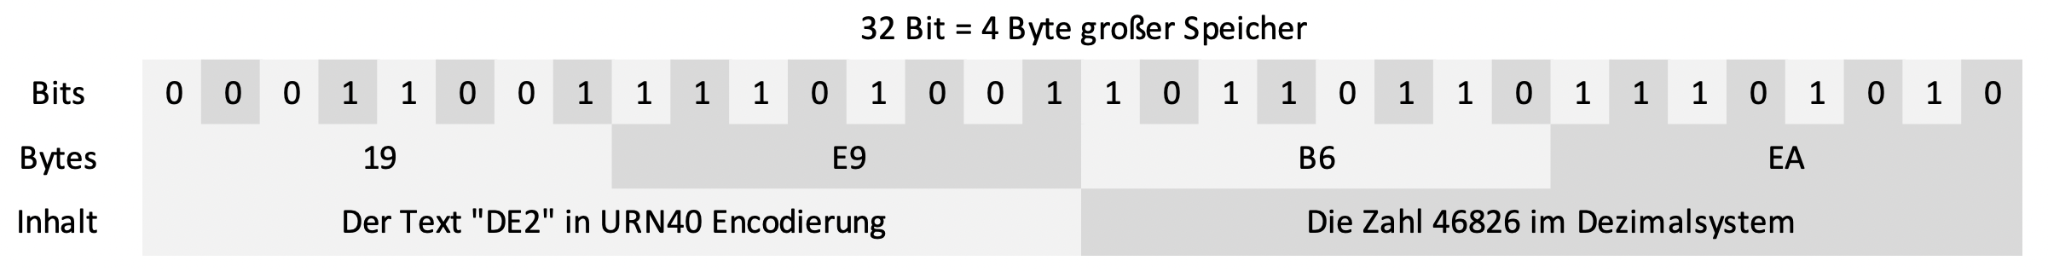
\includegraphics{media/rfid-tag.png}

}

\caption{\label{fig-speicher-rfid}Beispiel für einen Speicherbereich auf
einem RFID-Tag}

\end{figure}%

In Bibliotheken enthält das RFID-Tag auch ein sog. AFI-Bit (application
family indicator), das zur Medien- bzw.~Buchsicherung verwendet wird.
Komplexere Datenmodelle, wie das Dänische Datenmodell, brauchen deutlich
mehr Speicherplatz, um auf ein Tag zu passen.

\subsection{Steuerkommandos, Arten des
Zugriffs}\label{steuerkommandos-arten-des-zugriffs}

RFID-Geräte kommunizieren mit RFID-Tags über verschiedene sog.
Steuerkommandos. Analog zu Barcodes, die von einem Drucker gedruckt
werden (WRITE) und von einer Lesepistole eingelesen werden (READ), gibt
es ähnliche Steuerkommandos auch für RFID-Tags, wobei diese
entsprechende Kommunikation zwischen RFID-Gerät und Tag auslösen. Je
nach Technologie (HF, UHF bzw.~sogar nach technischer Spezifikation der
Tags, SLI, SLI-S, SLI-X) existieren verschiedene Kommandos, die
verschiedene Aktionen mit einem Tag auslösen. Ohne in technische Details
zu gehen, lassen sich diese Kommandos grob wie folgt abstrahieren: READ,
WRITE, SECURE, UNSECURE, KILL, PROTECT. Dies entspricht der natürlichen
Interaktion mit den Tags etwa beim Inventarisieren neuer Bücher (WRITE),
dem Verbuchen (READ, dann UNSECURE) oder dem Durchschreiten eines Gates
(prüfen auf SECURED).

Bei der Nutzung von Bibliotheksgeräten, die RFID einsetzen, kommt man im
Normalfall nicht mit den Steuerkommandos von RFID-Hardware in Berührung.
Sollte man aber mit der Hardware selber experimentieren oder testen,
wird man manchmal auch roh auf die Tags schreiben müssen.

\subsection{Sicherheit und
Datenschutz}\label{sicherheit-und-datenschutz}

RFID-Tags können auf zwei Arten manipuliert werden: Einerseits kann man
mittels geeigneter Hardware (im Falle von RFID-HF genügt ein Smartphone)
den Inhalt eines nicht schreibgeschützten Tags verändern. Dies betrifft
sowohl das Sicherungsbit (das Gate schlägt also nicht mehr an, wenn ein
so manipuliertes Medium herausgetragen wird), als auch den gesamten Tag
Inhalt, sodass das Medium von der Infrastruktur der Bibliothek nicht
mehr verarbeitet werden kann. Andererseits kann man die meisten UHF-Tags
und manche HF-Tags mit einem einfachen Befehl zerstören, also dauerhaft
und endgültig stummschalten. Beide Arten der Manipulation kann man mit
einem Passwortschutz wirkungsvoll verhindern (fun-fact: die meisten in
Deutschland eingesetzten HF-Systeme enthalten diesen Passwortschutz
nicht, sind also nicht vor einfachsten Manipulationen geschützt).

Bei der Einführung von RFID werden häufig Diskussionen zum Thema
Datenschutz geführt. Wenn allerdings die Tags lediglich mit einer nur
intern bekannten ID beschrieben werden, also einer ID, die nicht
öffentlich im Katalog des BMS einsehbar ist, besteht diese Gefahr nicht.
Selbst wenn jemand Medien im Rucksack eine*r Nutzer*in scannen würde
(was technisch nicht unaufwändig ist), könnte man daraus keine
Rückschlüsse auf das betreffende Medium schließen.

\subsection{Anbindung von RFID-Infrastruktur an
BMS}\label{anbindung-von-rfid-infrastruktur-an-bms}

Damit ein Gerät einer RFID-Infrastruktur mit dem Rest der Systeme einer
Bibliothek, insbesondere dem
\hyperref[bibliotheksmanagementsysteme]{BMS}, kommunizieren kann, muss
es über entsprechende Schnittstellen angebunden werden. Bei der
Anschaffung sollte daher darauf geachtet werden, dass die Anlage etwa
die standardisierten Schnittstellen wie SIP2 oder NCIP nutzt, um
Dienstleistungen wie Rückgabe, Sortierung und Ausleihe mit dem
Bibliothekssystem abwickeln zu können (Michaelis 2014).

Die Anbindung von lokalen RFID-Readern an Computerarbeitsplätzen von
Mitarbeiter*innen erfolgt im Regelfall durch das Anschließen eines
solchen Gerätes direkt am Arbeitsplatz, zumeist über USB. Es existieren
allerdings auch Reader, die über einen Netzwerkanschluss direkt mit dem
Netz der Einrichtung verbunden werden können und dadurch weitere
Flexibilität ermöglichen, da kein Gerät an einen lokalen Computer
angesteckt werden muss.

Im Vergleich zu Barcode-Lesern, die den Inhalt eines gelesenen Barcodes
meist einfach als Tastatureingaben an die Position des Cursors am
Bildschirm ausgeben, können RFID-Geräte aufgrund der komplexen Inhalte
von RFID-Tags (siehe \hyperref[datenmodelle]{Datenmodelle}) auch mittels
Programmierschnittstellen aus dem BMS oder anderen Systemen angesprochen
werden. Die Logik der Interpretation des Taginhalts liegt hierbei dann
beim BMS oder bei einer Zwischensoftware („Proxy``), die zwischen Reader
und BMS vermittelt.

\subsection{Medienarten}\label{medienarten}

RFID-Transponder sind nicht für alle Medienarten geeignet. Aufgrund der
Tatsache, dass RFID-Tags über Funkwellen mit Strom versorgt werden und
kommunizieren, gilt, dass die Tags durch das Vorhandensein von Metall,
Wasser, o.\,ä.~beeinflusst oder abgeschirmt werden können. Selten
vorkommende metallisch beschichtete Einbände von Bücher zum Beispiel
verhindern effizient die Nutzung von RFID. Konkret bedeutet das, dass
die Antenne eines RFID-Tags im Regelfall nicht mehr funktioniert, wenn
sie in direkter Nähe zu metallischen Oberflächen ist: Eine CD, ein
Laptop im Rucksack, oder sogar ein anderen RFID-Tag in einem dünnen
Buchstapel können die Reichweite und Lesbarkeit einschränken. Beim
Einbringen von Tags ist daher darauf zu achten, dass sie nicht auf
solche Materialien aufgebracht werden. Ebenfalls hilft es nicht, ein Tag
auf die Außenseite eines metallischen Gegenstands aufzubringen.

Generell sollte der Gegenstand, auf den ein Tag aufgebracht wird, von
Funkwellen durchdrungen werden können, zumindest aber von der Seite, an
der das Tag aufgebracht wurde.

Gleichzeitig bedeutet das auch, dass RFID-Tags durch das Vorhandensein
von Wasser, also Menschen, ebenfalls abgeschirmt werden können. Eine
hundertprozentige Erkennungsrate in einem Sicherheitsgate ist somit
unrealistisch.

RFID-Transponder sind natürlich nicht geeignet für Medien, bei denen
eine Unwucht störend ist (Schallplatten, CDs), sie sollten dabei auf der
Außenhülle angebracht werden. Bei CDs ist zusätzlich der Metallanteil
der CD störend.

Hinzu kommt, dass RFID-Tags unterschiedlicher Hersteller und Arten
unterschiedlich auf verschiedene Umgebungen reagieren. Für UHF wird vom
Unternehmen EECC eine Studie herausgegeben, die die physikalischen
Eigenschaften von verschiedenen Tags untersucht ({„{UHF} {RFID} Almanach
2022``} 2022). Um diese Studie nutzen zu können, sind allerdings
fundierte physikalische Kenntnisse notwendig, alternativ kann die Firma
mit der Aussprache einer Empfehlung beauftragt werden, wie 2019 in der
UB Dortmund geschehen.

Nach Einführung von RFID ist das Weiterführen von Barcodes zur
Identifikation zwar nicht mehr zwangsläufig erforderlich, es ergeben
sich aber zwei Vorteile, insofern weiterhin der Barcode mit am oder im
Medium angebracht wird. Durch den Barcode kann das Medium weiterhin
maschinenlesbar identifiziert werden. Falls RFID Komponenten ausfallen
sollten, kann mit dem Barcode traditionell weiter gearbeitet werden.
Wenn außerdem (wie meist üblich) unter dem Barcode auch die im Barcode
codierten Zeichen mit zu sehen sind, können auch Menschen das Medium
bzw.~den Band problemlos eindeutig identifizieren. Barcodes können dabei
auch auf ein mit Papier beschichtetes RFID-Tag aufgebracht werden.

Auf die Barcodes kann beim Einsatz von RFID auch verzichtet werden, wenn
in Kauf genommen wird, dass man für die Identifikation eines Buches eine
Recherche im BMS durchführen muss, wenn das Tag unlesbar oder falsch
beschrieben ist.

\subsection{Alternativen zu RFID in
Bibliotheken}\label{alternativen-zu-rfid-in-bibliotheken}

Fortgeschrittene Entwicklungen im Bereich Texterkennung (Optical
Character Recognition, OCR) und generell Computer Vision (CV) können es
ermöglichen, ganz ohne technisch lesbare Identifikationsmerkmale ein
Buch zu erkennen und zu verarbeiten. Bei einer solchen Lösung wird
mittels einer Kamera das Äußere eines Mediums aufgenommen und erkannt
und kann somit weiterverarbeitet werden. Um das Medium einer Bibliothek
zuzuordnen, kann weiterhin etwa ein Aufkleber auf dem Buch, z.\,B. ein
Signaturetikett auf dem Rücken, erkannt werden, um das Buch der
Bibliothek zuordnen zu können und ggf.~mehrere Exemplare auseinander
halten zu können.

Bisher ist kein solches System aktiv im Einsatz; die Erkennung von
Objekten ist jedoch ein aktives Forschungsthema.

Vollständige Automatisierung ist in Bibliotheken auch möglich mit
Barcodeverbuchung und EM-Sicherung (EM = elektro-magnetisch). Wenn die
Barcodes vorne außen am Buch angebracht sind, können sie auch von
Ausleihautomaten und Rückgabeautomaten gelesen und verarbeitet werden.
EM-Sicherung wird mittels magnetisierbaren Streifen realisiert, die mit
doppelt klebendem Film in den Falz der Bücher geklebt wird. Diese
Streifen sind über separate Geräte magnetisierbar
bzw.~entmagnetisierbar. Der Status ist detektierbar über spezielle
Gates, sodass darüber die Buchsicherung realisierbar ist. Auch diese
Sicherung ist natürlich fehleranfällig und nicht 100\%ig. Schon
metallene Gegenstände in derselben Tasche wie gesicherte Bücher
verhindern die Erkennung. Es gibt bei dieser Methode also keinen Vorteil
gegenüber eines RFID-Betriebs -- im Gegenteil, diese Technologie ist
veraltet, wird immer seltener genutzt und insofern immer teurer.

\section{Dienste für Nutzer*innen}\label{dienste-fuxfcr-nutzerinnen}

\subsection{Website}\label{website}

Eine Internetpräsenz ist für eine öffentliche Einrichtung mittlerweile
unabdingbar und dient vielen Nutzer*innen als Erstkontaktmöglichkeit,
Arbeitsmittel und Informationsplattform gleichermaßen. Die Infrastruktur
hierfür wird im Kapitel~\ref{sec-kommunikation} genauer behandelt.

\subsection{Internetzugang}\label{internetzugang}

Der kostenlose Zugang zum Internet ist für viele Nutzer*innen ein Grund,
die Bibliothek als Lern- und Arbeitsort zu nutzen.
\hyperref[]{PC-Arbeitsplätze} und freies WLAN gehören deshalb in den
meisten Bibliotheken mittlerweile zum Standard. Letzteres ist
Voraussetzung, um mit eigenen Geräten wie Notebook, Handy und Tablet
arbeiten zu können. Damit in allen relevanten Bereichen WLAN mit
angemessener Bandbreite verfügbar ist, sollten Bibliotheken
Anforderungen an die Ausstattung des Gebäudes mit einer ausreichenden
Anzahl an WLAN-Access-Points bestimmen. Das öffentliche Netz sollte vom
internen Netz für Mitarbeiter*innen der Bibliothek getrennt sein, um das
Risiko eines Angriffs auf die Infrastruktur zu minimieren. Bei
öffentlichen PCs sind zusätzlich Datenschutzmaßnahmen zu treffen.

Grundsätzlich sind für die Bereitstellung von Internet zwei Fragen zu
klären:

\begin{itemize}
\item
  Ist der Zugang offen oder sind ein Passwort und ggf.~Registrierung
  notwendig?
\item
  Erfolgt der Zugang direkt durch die Bibliothek oder per Roaming über
  Dritte?
\end{itemize}

In Hochschulen und Forschungseinrichtungen bietet sich die
WLAN-Roaming-Infrastruktur \href{https://eduroam.org}{eduroam}, die in
Deutschland vom DFN koordiniert wird und auch international an vielen
Bildungseinrichtungen verfügbar ist. Der Betrieb von eduroam wird in der
Regel durch das universitäre Rechenzentrum verantwortet. Nutzer*innen
müssen allerdings an einer Einrichtung registriert sein und ihre
Zugangsdaten eingeben, um eduroam zu verwenden.

Für den offenen Zugang kann im Idealfall mit der Trägereinrichtung
z.\,B.~der eigenen Kommune zusammengearbeitet werden. Eine weitere
Möglichkeit ist das ehrenamtliche Freifunk-Projekt. Je nach
Rahmenbedingung gibt es verschiedene Leitfäden und Fördermöglichkeiten
zur Einrichtung offenen Internetzugangs.

\begin{figure}

\centering{

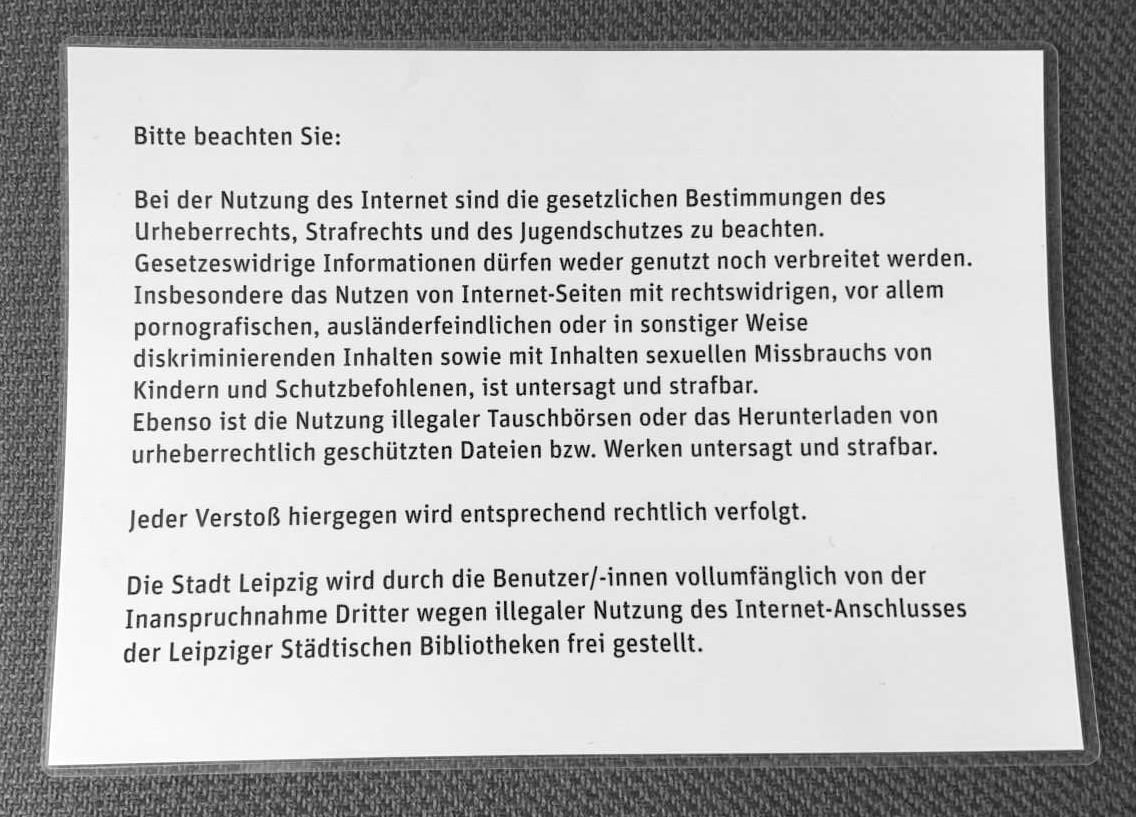
\includegraphics{media/internet-nutzungshinweise.jpg}

}

\caption{\label{fig-nutzungshinweis}Internet-Nutzungshinweise in den
Städtischen Bibliotheken Leipzig}

\end{figure}%

Als Anbieter von öffentlichem WLAN sollten Bibliotheken auf Gefahren und
mögliche Sicherheitsvorkehrungen hinweisen. Bei der Nutzung von
öffentlichem WLAN muss beachtet werden, dass die Verbindungen in der
Regel nicht verschlüsselt sind und somit alle, die sich im gleichen
Netzwerk befinden, potenziell die übertragenen Daten mitlesen können.
Zur Minimierung des Risikos sollten Webseiten möglichst nur
verschlüsselt per HTTPS aufgerufen werden und Datei- und
Verzeichnisfreigaben deaktiviert sein, um zu verhindern, dass andere
Teilnehmer im Netzwerk auf eigene Dateien zugreifen können.

\subsection{Gruppen- und
Einzelarbeitsplätze}\label{gruppen--und-einzelarbeitspluxe4tze}

Zur Ausstattung von Gruppen- und Einzelarbeitsplätzen gehört auch
angemessene Informationstechnik. Wesentlich sind zunächst ein stabiler
Internetzugang und genügend Steckdosen. Dabei sollte die Absicherung mit
ausreichenden Sicherungen und getrennten Stromkreisen vorgesehen werden,
da ein defektes Laptop-Netzteil sonst zum Ausfall der Sicherung eines
gesamten Lesesaals führen kann. Vor allem sollte in solchen Fällen nicht
plötzlich das gesamte Bibliothekspersonal stromlos dastehen.

Ausstattung, Verwaltung und Unterhalt von Räumen mit Technik ist
insbesondere für öffentliche Bibliotheken ressourcen- und
kostenintensiv. Entsprechend sollten sich Bibliotheken an der
tatsächlichen Nachfrage ihrer Nutzer*innen orientieren und nur die
Technik anschaffen, die sie selbst verwalten können.

Es gibt auch einige Bibliotheken, die in ihren öffentlichen
Arbeitsbereichen sogenannte Smartboards zur Verfügung stellen. Damit
sind große Monitore gemeint, die Computer enthalten. Die gewohnten
Funktionen wie Webbrowsing, Textverarbeitung und andere Programme sind
über Bildschirmtastatur/Touchscreen erreichbar, man kann aber auch eine
Art digitales Whiteboard nutzen und die darauf erarbeiteten Ergebnisse
digital weiternutzen.

In der Praxis zeigte sich jedoch bisher, dass Smartboards meistens nur
als großer Monitor mit extern angeschlossenem Notebook oder integriertem
Computer genutzt werden. Ein Angebot von derartigen Projektionsflächen
lässt sich auch kostengünstiger realisieren.

In einigen Bibliotheken werden auch komplette Workspaces für große
Gruppen angeboten. Für die gezielte Nutzung von speziell ausgestatteten
Arbeitsplätzen kann das Angebot einer Sitzplatz- bzw.~Raumbuchungslösung
nützlich sein. Das Buchungssystem lässt sich auf der Homepage oder in
einer Service-App einbinden und kann auf diesem Weg ebenso wie andere
Dienstleistungen genutzt werden. Hier werden inzwischen auch gehostete
Lösungen als Cloud-Service angeboten. Oft unterstützen diese Dienste die
Anmeldung via Shibboleth und OpenID-Connect, ggf.~sogar die Nutzung
innerhalb einer Föderation. Die Fragen des Datenschutzes sind natürlich
bei einem solchen Einsatz im Vorfeld zu klären.

\subsection{Öffentliche
PC-Arbeitsplätze}\label{uxf6ffentliche-pc-arbeitspluxe4tze}

Sowohl wissenschaftliche als auch öffentliche Bibliotheken bieten
PC-Arbeitsplätze für ihre Nutzer*innen an. Auch wenn der Trend zu
eigenen Geräten geht, bleiben die Nutzungszahlen bei den
PC-Arbeitsplätzen besonders in öffentlichen Bibliotheken stabil.

Dienste wie die Nutzung des Internets und Textverarbeitung mit oder ohne
Gebühren sind die häufigsten Einsatzzwecke für PC-Arbeitsplätze und
sollten weiterhin niedrigschwellig angeboten werden. Die
Gebührenabrechnung für angemeldete Nutzer*innen erfolgt über
\hyperref[]{Bezahlsysteme}, die an das Bibliotheksmanagementsystem
angegliedert sind. Geräte mit Bargeld- oder Kartenzahlung bieten
außerdem die Möglichkeit, diese auch ohne Bibliotheksmitgliedschaft zu
nutzen.

In der Regel stehen PC-Arbeitsplätze angemeldeten Nutzer*innen zur
Verfügung. Anhand der Benutzergruppe können altersbedingte
Einschränkungen vorgenommen werden. So müssen Eltern z.\,B.~der
Internetnutzung von minderjährigen Kindern zustimmen.

Bei kostenfreier und nicht reglementierter Nutzung muss der Jugendschutz
besonders beachtet werden. Denkbar ist dabei das Whitelisting von
Internetseiten, d.\,h.~eine Freischaltung von Seiten, die aus
Jugendschutzsicht als unbedenklich eingestuft wurden. Ein Blacklisting
hingegen ist nicht empfohlen, da keinesfalls alle bedenklichen Seiten
bekannt sein können.

Auch der Datenschutz spielt im öffentlichen Bereich eine große Rolle.
PCs müssen so konfiguriert werden, dass Nutzer*innen ausschließlich ihre
eigenen Dateien sehen und keinen Zugriff auf Dateien von anderen
Personen erhalten. Dies wird z.\,B.~durch persönliche Nutzerprofile
(gebunden an das Benutzerkonto) oder systemseitige Rücksetzung aller
Einstellungen (Gastzugänge) erreicht. Zum Betrieb solcher
„Kiosksysteme`` gibt es entsprechende Software. Der Einsatz von
Thin-Clients als zentral verwaltete Terminals dienen, die weder
Programme noch Daten lokal speichern, ist in diesem Bereich sinnvoll.

Auch bei der Freigabe der Nutzung von Speichermedien sollten
Sicherheitsvorkehrungen getroffen werden, beispielsweise vorgeschaltete
automatische Virenprüfungen. Eine Sperre von externen Speichermedien
wäre ebenfalls denkbar, jedoch spricht die aktuelle Nachfrage dagegen.

Hinweise zur Einrichtung eines öffentlichen WLAN in Bibliotheken gibt
der Abschnitt zum \hyperref[internetzugang]{Internetzugang}.

\subsection{Digitalisieren/Scannen, Digitalisierung on
demand}\label{digitalisierenscannen-digitalisierung-on-demand}

Scannen, Kopieren und Drucken sind weitere häufig genutzte Angebote in
Bibliotheken. Zur Unterstützung von Nachhaltigkeit und Digitalisierung
von Studium und Lehre könnte das Ausdrucken auf Papier reduziert oder
gar nicht angeboten werden und stattdessen das Einscannen auf
Datenträger oder Speichersysteme befördert werden.

Um Nutzer*innen das Digitalisieren von Medien zu ermöglichen, kann eine
Bibliothek Scanner zur Verfügung stellen. Im einfachsten Fall sind das
Multifunktionsgeräte (MFGs), die sowohl Kopier- als auch Scan- und
Druckfunktionen anbieten. Meistens sind Druck- und Kopierfunktionen
kostenpflichtig, Scannen oft kostenfrei. Höherwertige Scans von größeren
Vorlagen und ergonomisches Scannen sind mit sogenannten Kopfscannern
möglich. Bei diesen Scannern liegt das Medium offen, mit dem Druckbild
nach oben auf der Vorlagefläche. Mit Fingerdruck oder Fußschalter wird
der Scanvorgang ausgelöst, anschließend kann ohne Umdrehen der Vorlage,
wie es bei einem herkömmlichen Kopierer notwendig wäre, umgeblättert
werden.

Ein weiterer Anwendungsfall ist das Einscannen von Einzelblattvorlagen.
z.\,B.~Vorlesungsmitschriften. Hier sind Scanner mit automatischem
Papiereinzug ideal, die Vorder- und Rückseite gleichzeitig einscannen
können.

Das Digitalisat kann in der Regel auf einem USB-Stick gespeichert
werden. Komfortabler sind eine Netzwerkverbindung und eine
Anmeldemöglichkeit für Nutzer*innen. Alternativ kann auch die Eingabe
einer Mailadresse mit anschließendem Versand eines Links auf das
Dokument angeboten werden. Das Digitalisat selbst per E-Mail zu
verschicken ist i.\,d.\,R.~aufgrund der Dateigröße nicht möglich.

\subsection{Ausleihbare Geräte}\label{ausleihbare-geruxe4te}

Als „Bibliothek der Dinge`` wird die Möglichkeit bezeichnet, in
Bibliotheken auch Gegenstände wie Werkzeuge, Sportgeräte und
Musikinstrumente ausleihen zu können. Für die Ausleihe von Kunstwerken
oder Spielen sind auch die Begriffe „Artothek`` bzw.~„Ludothek`` üblich.
Für diese Gegenstände ist in der Regel eine besondere Form der
\hyperref[mediensicherung]{Mediensicherung} notwendig. Für die Ausgabe
von Tablets gibt es beispielsweise spezielle Automaten. Durch Verbindung
mit dem Bibliotheksmanagementsystem ist es auch möglich, die Freigabe an
ein Mindestalter zu knüpfen und verschiedene Profile auf den Tablets
anzulegen.

\subsection{Makerspace}\label{makerspace}

Ein Makerspace ist ein Bereich in einer Bibliothek, in dem Hardware und
Software zum Ausprobieren zur Verfügung gestellt wird. Ziel ist das
Angebot eines niedrigschwelligen Zugangs zu neuen (technischen)
Entwicklungen, die der breiten Öffentlichkeit~-- in der Regel aus
Kostengründen~-- sonst nicht zur Verfügung stehen. Beispiele für
Angebote in Makerspaces sind:

\begin{itemize}
\item
  3D-Drucker
\item
  Geräte zur Holz/Metallverarbeitung
\item
  Stickmaschine/Nähmaschine
\item
  Ton- und Videotechnik
\item
  Repair-Café
\end{itemize}

Zusätzlich zur Bereitstellung der Technik bieten viele Bibliotheken
Einführungs- und Expertenkurse an, die jedoch auch stark von den
vorhandenen Personalressourcen abhängig sind. Makerspaces sind vor allem
in größeren öffentlichen Bibliotheken verbreitet. Auch in einigen
wissenschaftlichen Bibliotheken gibt es inzwischen entsprechende
Angebote, wobei hier der Fokus mehr auf dem Einsatz in Lehre und Lernen
liegt, zum Beispiel das Dortmunder
\href{https://hylec.tu-dortmund.de/}{Hybrid Learning Center (hylec)}.

\subsection{Bibliotheks-App}\label{bibliotheks-app}

Bei Überlegungen zum Einsatz einer App für die Dienstleistungen der
Bibliothek sollten verschiedene Aspekte betrachtet werden. Eine App wird
um so häufiger installiert, je mehr wichtige und häufig genutzte
Funktionalitäten damit nutzbar sind. Eine Integration der
Dienstleistungen der Bibliothek in eine bestehende App der
übergeordneten Institution ist also der Eigenentwicklung vorzuziehen~--
sofern das möglich ist.

In einer App können grundsätzlich alle Dienstleistungen der Bibliothek
angeboten werden. Ein Mehrwert entsteht dann, wenn man den mobilen
Charakter des Endgerätes berücksichtigt. Beispiele: Navigation in der
Bibliothek mit Wegweisung am Endgerät, Buchung des Gruppenarbeitsraums,
vor dem man gerade steht (z.\,B.~über einscannbare QR-Codes).

Eine vollständige Nutzung der Dienstleistungen der Bibliothek ist nur
dann möglich, wenn man sich auch digital anmelden kann. Es sollte also
eine Form eines digitalen Ausweises geben, Accountname/Passwort im
einfachsten Fall, komplett digitaler Ausweis über die App im besten
Fall.

Wildau als Beispiel mit UNIDOS hat eine Integration des
Bibliothekskontos, mit der Möglichkeit der Anzeige aller entliehenen
Medien und der Verlängerung dieser. Bewerkstelligt wird die Funktion via
SIP2-Schnittstelle. Zusätzlich können Discovery-Systeme sowie eine
Raumbuchung verlinkt bzw.~direkt via App ermöglicht werden. Die Kosten
für die Entwicklung einer nativen App für Android und iOS sind eher
hoch. Daher kann stattdessen auch eine responsive Web-App zum Einsatz
kommen. Apps machen meist nur dann wirklich Sinn, wenn man Zugriff auf
interne Komponenten der Smartphones wie NFC, Kamera (zum Scannen),
Bluetooth (z.\,B.~zur Detektion von Beacons) etc. benötigt.

\subsection{Technische Beratung und
Schulungen}\label{technische-beratung-und-schulungen}

Technische Beratung erfolgt oft in dem Umfang, der für lokale
Bibliotheksdienste sinnvoll ist. Bietet eine Bibliothek technische
Dienste wie z.\,B.~die Onleihe an, werden sich Nutzer*innen bei Fragen
direkt an die Bibliothek statt an den Dienstleister. Typische Bedarfe
umfassen unter Anderem:

\begin{itemize}
\item
  Erklärung und Dokumentation zu Diensten, z.\,B.~E-Book-Leihe,
  Streaming-Dienste, E-Learning-Ressourcen
\item
  E-Book-Reader Beratung zur Unterstützung der E-Book-Ausleihe
\item
  Beratung zu App-Nutzung, die als digitale Inhalte angeboten werden
\end{itemize}

Die Mitarbeiter*innen in der Bibliothek müssen sich daher stetig
fortbilden, um ihren Nutzer*innen einen guten Service zu bieten. Werden
neue Dienste eingeführt, bedarf es neben der Werbung auch einer
Einführung oder dem Angebot einer Schulung, in erster Linie für
Mitarbeiter*innen. Viele Anbieter unterstützen dabei mit eigenem
Schulungsmaterial, was unter Umständen je nach Zielgruppe angepasst
werden muss.

\section{Dienste für
Mitarbeiter*innen}\label{dienste-fuxfcr-mitarbeiterinnen}

Die folgenden IT-Dienstleistungen dienen der Unterstützung der täglichen
Arbeit, insbesondere im Hinblick auf verteilte Arbeitsumgebungen und
mobiles Arbeiten. In vielen Fällen werden sie von der übergeordneten
Einrichtung einer Bibliothek bereitgestellt. Neben dem Zugang zu
Arbeitsmitteln dienen die Dienste vor allem der internen Kommunikation
und dem Wissenmanagement (Kapitel~\ref{sec-kommunikation}).

\begin{tcolorbox}[enhanced jigsaw, leftrule=.75mm, toprule=.15mm, left=2mm, opacityback=0, arc=.35mm, colback=white, breakable, colframe=quarto-callout-important-color-frame, rightrule=.15mm, bottomrule=.15mm]
\begin{minipage}[t]{5.5mm}
\textcolor{quarto-callout-important-color}{\faExclamation}
\end{minipage}%
\begin{minipage}[t]{\textwidth - 5.5mm}

\textbf{Wissensmanagement} besteht aus
\hyperref[wissensmanagement]{Prozessen} zur Erfassung und Weitergabe von
Wissen innerhalb einer Organisation, das oft nur implizit in den Köpfen
der Mitarbeitenden vorliegt. Werkzeuge hierfür werden im
Kapitel~\ref{sec-kommunikation} vorgestellt.

\end{minipage}%
\end{tcolorbox}

\subsection{Mobiles Arbeiten}\label{mobiles-arbeiten}

Für mobiles Arbeiten müssen Endgeräte transportabel sein und die
Dienste, die für das Arbeiten notwendig sind, müssen vom jeweiligen
Standort aus erreichbar sein (siehe \hyperref[vpn]{VPN}). Für
dauerhaftes Arbeiten von anderer Stelle als dem Büro (Homeoffice) ist
aus Ergonomiegründen ein fester Arbeitsplatz mit Tastatur, Maus,
Bildschirm und ggf.~Anschlussmöglichkeit für mobile Geräte („Dock``)
vorzuziehen oder vorgeschrieben.

Der Begriff \emph{bring your own device} (BYOD) bezeichnet die Nutzung
von privaten Endgeräten in der Infrastruktur des Arbeitgebers. Dies ist
allerdings mit einigen Herausforderungen verbunden. So kann nicht
zentral sichergestellt werden, dass das Endgerät frei von Schadsoftware
ist. Auch die Sperrung des Gerätes aus der Ferne ist nicht möglich (auf
eigenen Geräten des Arbeitgebers kann eine solche Software installiert
werden, die im Falle eines Diebstahls aktiviert werden kann).
Letztendlich liegt also die Verantwortung dafür, ob dienstliche Daten
über das private Gerät in falsche Hände gelangen, beim Arbeitnehmer.

\subsection{VPN}\label{vpn}

Ein „Virtuelles Privates Netzwerk`` dient dazu, über einen
authentifizierten Zugriff das Endgerät der Mitarbeiter*innen
bzw.~Nutzer*innen virtuell in das interne Netzwerk (Intranet) der
Institution einzubinden. Das ermöglicht die Nutzung von Diensten, die
auf der Basis der Netzwerkadresse (IP-Adresse) entscheiden, ob der
Zugriff ermöglicht wird. Viele Dienste einer Institution werden aus
Sicherheitsgründen über eine \emph{Firewall} dem gesamten Internet
verborgen und sind nur über ein VPN auch außerhalb der Institution, zum
Beispiel aus dem Homeoffice, zugreifbar.

\subsection{Werkzeuge zur
Kommunikation}\label{werkzeuge-zur-kommunikation}

Wie im Kapitel~\ref{sec-kommunikation} beschrieben, gibt es verschiedene
Werkzeuge zur synchronen und asynchronen Kommunikation von Telefon über
E-Mail und Chats bis zu Videokonferenzsystemen. Neben der reinen
Kommunikation dienen Werkzeuge wie Wikis und Ticketsysteme auch der
Zusammenarbeit und kollaborativen Erstellung von Inhalten.

Um virtuelle Besprechungsräume so auszustatten, dass auch Menschen an
Besprechungen teilnehmen können, die nicht anwesend sind, ist technische
Infrastruktur erforderlich. Die Abwesenden müssen für die Anwesenden
sichtbar und hörbar sein, ohne dass die Anwesenden Headsets tragen
müssen. Dies erreicht man mit Webcams, die automatisch auf die
sprechende Person fokussieren und im Idealfall auch Störgeräusche
(Echos, Rauschen, Rascheln) ausblenden. Die gängigen Systeme im knapp
vierstelligen Eurobereich genügen für Konferenzen mit bis zu sechs
anwesenden Personen um einen Tisch herum. Sind mehr Personen anwesend,
steigt der technische Aufwand stark an, wenn häufig hybrid gearbeitet
wird und die abwesenden Personen nicht benachteiligen werden sollen.

\subsection{Fileservices}\label{fileservices}

Dienstlich genutzte Dateien sollten an zentraler Stelle abgelegt werden,
damit sie in eine Backup-Lösung eingeschlossen werden können und damit
die Möglichkeit besteht, sie mit anderen Menschen auszutauschen.
Entweder wird dazu als Netzlaufwerk ein klassischer Fileserver wie zum
Beispiel \emph{Windows Server} genutzt, oder es kommt eine
\hyperref[echtzeit-kollaboration]{Cloudlösung} wie \emph{Nextcloud} zum
Einsatz. Zusätzlich oder alternativ kann ein
\hyperref[dokumentenmanagementsysteme]{Dokumentenmanagementsystem}
genutzt werden.

\subsection{Dokumentenmanagementsystem
(DMS)}\label{dokumentenmanagementsysteme}

Dokumentenmanagementsysteme sind Multi-User Softwaresysteme mit
Anbindung an eine hinreichend großen und ausfallsicheren Datenspeicher.
Sie lösen in der Regel drei Anforderungen:

\begin{itemize}
\item
  langfristige ggf.~auch revisionssichere Ablage digitalisierter oder
  rein digitaler Dokumente die einer Aufbewahrungsfrist unterliegen
  (Archivierung, Versionierung)
\item
  Unterstützung der Datenverarbeitung für Prozesse zwischen
  verschiedenen Akteuren (Workflows)
\item
  Strukturierung und Pflege der Dokumente institutionsrelevanter
  interner und externer Prozesse (Aktenplan)
\end{itemize}

Ab und an erhalten Bibliotheken den Auftrag, die Originale von
digitalisierten und in einem DMS abgelegten Dokumenten physisch zu
archivieren oder auch den Digitalisierungsprozess zu verantworten.
Hierbei ist es empfehlenswert, zwischen unternehmens-
bzw.~institutionskritischen Dokumenten, die nicht für die
Bibliotheksnutzer verfügbar sein sollen, und Dokumenten mit
bibliothekarischem Bezug zu unterscheiden, denn eine Bibliothek ist im
Allgemeinen kein Archiv.

\subsection{Social Intranet}\label{social-intranet}

Als Kombination des klassischen Intranets mit sozialen und
kommunikativen Funktionen ermöglicht ein Social Intranet den
Mitarbeitenden den einfachen Austausch von Informationen und Ideen und
wird genauer in Kapitel zur Kommunikation
(Kapitel~\ref{sec-kommunikation}) beschrieben.

\subsection{Planungs- und Koordinationstools}\label{sec-planungstools}

Die in diesem Absatz beschriebenen Werkzeuge dienen der
Aufgabenkoordination in der Bibliothek. Je mehr Personen in einem Team
an gemeinsamen Aufgaben arbeiten, desto empfehlenswerter ist der Einsatz
folgender Instrumente für die Aufgabenkoordination und das
Wissensmanagement in der Bibliothek.

\textbf{Ticketsystem}: Ticketsysteme dienen der strukturierten,
regelbasierten (z.\,T. automatischen) Abarbeitung von Anfragen,
Wünschen, Fehlermeldungen von Nutzenden. Diese Systeme können für alle
anfallenden Aufgaben innerhalb der Bibliothek verwendet werden,
z.\,B.~in der Softwareentwicklung (Kapitel~\ref{sec-anforderungen}) bei
der Bearbeitung von Kundenanfragen oder internen Prozessen.

Ein Vorteil ist die transparente Bearbeitung von Vorgängen, da sowohl
der Status als auch die Bearbeitenden jederzeit einsehbar und
nachvollziehbar sind. Statusänderungen werden dem Autor je nach
Einstellung des Ticketsystems automatisiert mitgeteilt. Alle
Bearbeiter:innen haben zu jeder Zeit Einblick und können bei Bedarf
übernehmen. Eine Vertretungsregelung oder E-Mail-Weiterleitung wird
damit obsolet. Nach abschließender Bearbeitung werden Tickets in der
Regel archiviert und können später zu Statistik- und
Dokumentationszwecken ausgewertet werden. Auch eine Art FAQ kann durch
entsprechend markierte Tickets erstellt werden. Beispiele:

\begin{itemize}
\tightlist
\item
  \emph{Redmine} (Open Source)
\item
  \emph{Jira} (kommerziell)
\item
  Integrierte Issue-Tracker im Rahmen der Softwareentwicklung,
  beispielsweise in \emph{GitLab} (Open Source) und \emph{GitHub}
  (kommerziell)
\end{itemize}

\textbf{Kanban-Board}: Ein Kanban-Board visualisiert jegliche
Arbeitsabläufe anhand einer in Spalten unterteilten Tafel (z.\,B.
Backlog, in Arbeit, fertig). Physisch ist dies mit Post-Its und
Whiteboard machbar. Ein Kanban-Board kann auch als Grundlage für ein
Projektmanagement nach SCRUM dienen. Beispiele:

\begin{itemize}
\tightlist
\item
  \emph{\href{https://apps.nextcloud.com/apps/deck}{Deck}} (Open Source
  Plugin für NextCloud)
\item
  \emph{\href{https://kanboard.org/}{Kanboard}} (Open Source)
\item
  \emph{\href{https://trello.com/}{Trello}} (kommerziell)
\end{itemize}

\textbf{Interne und externe Kalender:} Kalender können unterschiedliche
Aufgaben erfüllen. Intern helfen zwischen Mitarbeitenden geteilte
Kalender bei der Terminplanung und Abstimmung. Auf der
Bibliothekswebsite veröffentlichte Kalender können z.\,B.~buchbare
Veranstaltungen für Kund*innen und Besucher*innen der Bibliothek
enthalten. Ebenso ist eine Reservierung von Räumen oder Technik denkbar.
Verbunden mit einem Ticketverkauf oder einer Ticketreservierung können
sie die umständliche Kommunikation über E-Mails ablösen und ersparen
damit einen großen Verwaltungsaufwand. Beispiele:

\begin{itemize}
\tightlist
\item
  \emph{\href{https://www.supersaas.de/}{SuperSaaS}} (kommerziell)
\item
  \emph{\href{https://apps.nextcloud.com/apps/calendar}{Nextcloud
  Calendar}} (Open Source)
\end{itemize}

\textbf{Social Media Planung:} Betreibt eine Bibliothek mehrere Social
Media Kanäle, kann ein einziges Tool zur Planung und Veröffentlichung
von Beiträgen sinnvoll sein. Damit kann der Content zeitlich und
inhaltlich vorgeplant werden. Integrierte Analysewerkzeuge helfen zudem
bei der Zeitplanung, indem die vergangenen Veröffentlichungen
ausgewertet werden und der beste Zeitpunkt für die Zielgruppe ermittelt
wird. Beispiele:

\begin{itemize}
\tightlist
\item
  \emph{\href{https://www.hootsuite.com/}{Hootsuite}} (kommerziell, in
  der Basisversion frei nutzbar)
\item
  \emph{\href{https://buffer.com/}{Buffer}} (kommerziell, in der
  Basisversion frei nutzbar)
\item
  \emph{\href{https://trello.com}{Trello}} (kommerziell, in der
  Basisversion frei verfügbar)
\item
  \emph{\href{https://fedica.com/}{Fedica}} (kommerziell, in der
  Basisversion frei verfügbar)
\end{itemize}

\textbf{Wissenslandkarte}: Wissens(land)karten oder Knowledge Maps sind
grafische Verzeichnisse von Wissensträgern in Organisationen. Sie dienen
vor allem der Identifikation von Wissen in Unternehmen, um
Arbeitsabläufe effektiver und effizienter zu gestalten und referenzieren
auf Expertenwissen, Teamwissen, Wissensentwicklungsstationen sowie
organisationale Fähigkeiten und Abläufe. Bei dieser Methode wird
lediglich der Verweis auf das verankerte Wissen geliefert und nicht das
Wissen selbst dort abgelegt. Zur Erstellung können Mind-Mapping-Tools
verwendet werden.

\textbf{Terminfindung:} Abseits von Kalendern in E-Mail-Programmen
können Terminfindungstools sinnvoll sein, insbesondere bei der Planung
mit externen Beteiligten. Beispiele:

\begin{itemize}
\tightlist
\item
  \emph{\href{https://terminplaner.dfn.de/}{DFN terminplaner}}
\item
  \emph{\href{https://nuudel.digitalcourage.de/}{nuudel}}
\end{itemize}

\section{Zusammenfassung und
Ausblick}\label{zusammenfassung-und-ausblick}

Die technische Infrastruktur bildet die Grundlage für die Dienste einer
Bibliothek. Während sich die grundlegenden Dienste für Mitarbeiter*innen
einer Bibliothek nicht wesentlich von denen anderen Einrichtungen
unterscheiden, sind viele Dienste für die Nutzer*innen von Bibliotheken
an die Verwaltung physischer Medien gekoppelt.

\bookmarksetup{startatroot}

\chapter{IT-Management}\label{sec-management}

\begin{tcolorbox}[enhanced jigsaw, leftrule=.75mm, toprule=.15mm, left=2mm, opacityback=0, arc=.35mm, colback=white, breakable, colframe=quarto-callout-note-color-frame, rightrule=.15mm, bottomrule=.15mm]
\begin{minipage}[t]{5.5mm}
\textcolor{quarto-callout-note-color}{\faInfo}
\end{minipage}%
\begin{minipage}[t]{\textwidth - 5.5mm}

\vspace{-3mm}\textbf{Zusammenfassung}\vspace{3mm}

Dieses Kapitel beschreibt die Einführung und den
\hyperref[sec-betriebsmodelle]{Betrieb} von IT-Systemen über den
gesamten \hyperref[it-lebenszyklus]{Lebenszyklus} hinweg.

\end{minipage}%
\end{tcolorbox}

\section{Einleitung}\label{einleitung-2}

Grundsätzlich unterscheidet sich das Management von Informationssystemen
in und für Bibliotheken nicht sehr von Softwareentwicklung und Betrieb
in anderen Bereichen: IT-Systeme sind selten statisch, sondern folgen
einem \hyperref[it-lebenszyklus]{Lebenszyklus} von der Planung ihrer
Einführung bis zu ihrer Ablösung. Während des
\hyperref[sec-betriebsmodelle]{Betriebs} der Systeme müssen mögliche
\hyperref[betriebssicherheit-und-risikomanagement]{Risiken} beachtet und
\hyperref[rechtliche-rahmenbedingungen]{rechtliche Rahmenbedingungen}
eingehalten werden. In Bibliotheken sind daher entsprechende
\hyperref[kompetenzen]{IT-Kompetenzen} und ein
\hyperref[organisation]{organisatorischer Rahmen} für die
\hyperref[digitale-souveruxe4nituxe4t]{Digitale Souveränität} gefordert.
Um diesen Anforderungen begegnen zu können, gibt es Möglichkeiten zur
\hyperref[aus--und-weiterbildung]{Aus- und Weiterbildung}. Treiber der
jüngsten Entwicklung im IT-Bereich wissenschaftlicher Bibliotheken sind
Themen wie Digitalisierung (Kapitel~\ref{sec-digitalisierung}) und
forschungsnahe Dienste (Kapitel~\ref{sec-forschungsnahe-dienste})
während das Management von Bibliotheksmanagementsystemen
(Kapitel~\ref{sec-bibliotheksmanagementsysteme}) und Discovery-Systemen
(Kapitel~\ref{sec-discovery}) weitgehend etabliert sind.

\section{Lebenszyklus von IT-Systemen}\label{it-lebenszyklus}

Alle IT-Systeme folgen einem Lebenszyklus, der mit ihrer Einführung
beginnt und irgendwann mit ihrer Ablösung endet
(Abbildung~\ref{fig-it-zyklus}). Die wesentlichen Phasen im klassischen
Lebenszyklus eines IT-Systems werden im Folgenden näher betrachtet.
Darüber hinaus wird erläutert, wie Änderungen an IT-Systemen in
Institutionen im Rahmen des \hyperref[change-management]{Change
Managements} begleitet werden sollten.

Die konkrete Abfolge vor allem der ersten Phasen kann je nach der
angewendeten Projektmanagement-Methode (agil vs.~klassisch) variieren.
Eine Diskussion von agilen und klassischen Methoden liegt außerhalb des
Fokus dieses Handbuchs.

\begin{figure}

\centering{


\includegraphics[width=0.6\textwidth,height=\textheight]{index_files/mediabag/media/sdlc-sw.pdf}

}

\caption{\label{fig-it-zyklus}Softwareentwicklungs-Lebenszyklus}

\end{figure}%

\subsection{Planung und Analyse}\label{planung-und-analyse}

Grundlage für die Umsetzung eines Softwareprojekts, egal ob es sich um
individuell erstellte Software oder die Anpassung eines existierenden
IT-Systems handelt, ist ein gemeinsames Verständnis für das Ziel und die
Anforderungen an das Projekt. Dieses gemeinsame Verständnis,
insbesondere der Anforderungen, sollte bei allen Projektmitgliedern und
den weiteren Stakeholdern vorhanden sein. Die Anforderungen werden
idealerweise vor und während der Entwicklung unter Einbeziehung von
Nutzer*innen ermittelt und angepasst (Kapitel~\ref{sec-anforderungen}).

Zur Planungs- und Analysephase gehören neben einer grundsätzlichen
Machbarkeitsanalyse des Projekts die Zusammenstellung eines geeigneten
Teams, die Bestimmung der Stakeholder sowie die Klärung finanzieller und
rechtlicher Rahmenbedingungen.

\(\Rightarrow\) \emph{Siehe auch
\hyperref[entscheidungsprozess]{Entscheidungsprozess bei Einführung
eines BMS (Kapitel 7)}}

\begin{tcolorbox}[enhanced jigsaw, leftrule=.75mm, toprule=.15mm, left=2mm, opacityback=0, arc=.35mm, colback=white, breakable, colframe=quarto-callout-tip-color-frame, rightrule=.15mm, bottomrule=.15mm]
\begin{minipage}[t]{5.5mm}
\textcolor{quarto-callout-tip-color}{\faLightbulb}
\end{minipage}%
\begin{minipage}[t]{\textwidth - 5.5mm}

Zuweilen kommt es vor, dass die Entscheidung für ein IT-System bereits
getroffen ist, bevor geklärt wurde, welches Problem damit gelöst werden
soll. Auch in diesem Fall ist es sinnvoll, die Einführung mit einer
offenen Planung und Anforderungsanalyse zu beginnen, und danach zu
prüfen, welche Anforderungen das System tatsächlich abdecken kann.

\end{minipage}%
\end{tcolorbox}

\subsection{Design/Prototyping}\label{designprototyping}

Während der Design- bzw.~Prototyping-Phase entwickeln Designer*innen und
Entwickler*innen erste Prototypen des geplanten IT-Systems. Ziel ist es
dabei, Feedback der verschiedenen Stakeholder zu erhalten, um gemeinsam
ein besseres Verständnis der Anforderungen zu erhalten bzw.~diese zu
präzisieren. Kapitel~\ref{sec-anforderungen} geht gesondert auf die
Bedeutung dieser Einbeziehung und die damit verbundenen Methoden ein.

\subsection{Implementierung}\label{implementierung}

Aufbauend auf einem gemeinsamen Verständnis der Anforderungen überführen
Entwickler*innen Prototypen in lauffähigen Code. Wird im Rahmen des
Projekts ein bestehendes System implementiert, werden die Prototypen
zunächst in eine Testinstanz und in der Folge in die produktive Instanz
des Systems überführt.

In klassischen Projekten sieht man in dieser Phase zuerst ein Produkt
mit idealerweise schon möglichst vielen der gewünschten Features,
während nutzer*innenorientierte Vorgehensmodelle
(Kapitel~\ref{sec-anforderungen}) hier auf einen iterativen Prozess
setzen, welcher Produktweiterentwicklungen kontinuierlich bereitstellt
und evaluiert.

Unabdingbar sind der Einsatz eines Versionskontrollsystems (in der Regel
\emph{git}), Issue-Tracker und automatische Tests und Deployment
(kontinuierliche Integration), sodass Änderungen am Quellcode direkt zu
einer Aktualisierung der Test- und/oder Produktiv-Instanz der
installierten Software führen.

\subsection{Test und Integration}\label{test-und-integration}

Als letzte Lebensphase vor der Produktivschaltung werden Abnahmetests
und die Integration des entwickelten bzw.~erworbenen Systems in die
Zielumgebung durchgeführt. Im Falle der Inanspruchnahme eines
Dienstleisters wird hier auch dessen Leistung final abgenommen, wenn das
System erfolgreich produktiv in Betrieb genommen werden kann und alle
Anforderungen korrekt umgesetzt sind.

\subsection{Wartung}\label{wartung}

Die Wartungsphase folgt auf die Produktivsetzung des IT-Systems. In
dieser Lebensphase wird das System nicht mehr grundlegend
weiterentwickelt, es werden jedoch Fehler (Bugs) entfernt und
Anpassungen der Funktionsweise im Sinne der Parametrisierung oder eine
Optimierung der Programmabläufe vorgenommen.

Typischerweise verbleiben IT-Systeme, die grundlegende Geschäftsprozesse
abbilden oder die nach individuellen Anforderungen erstellt wurden,
viele Jahre in dieser Phase (siehe Beispiel
Abbildung~\ref{fig-verweildauer}).

\begin{figure}

\centering{


\includegraphics{index_files/mediabag/media/lifespan-sw.pdf}

}

\caption{\label{fig-verweildauer}Lebenszeit (in Jahren) einiger
ausgewählter Nachweissysteme der Staatsbibliothek zu Berlin, die Stand
2022 erst teilweise abgelöst wurden.}

\end{figure}%

\subsection{Ablösung}\label{abluxf6sung}

Die Ablösung eines Systems kann eine Vielzahl an Gründen haben. So
entwickeln sich die technischen Möglichkeiten und die Anforderungen der
Nutzer*innen kontinuierlich weiter. Eine Ablösung kann aber auch durch
technische Obsoleszenz erzwungen werden, wenn zugrundeliegende
Software-Komponenten wie das Betriebssystem oder ein
Datenbankmanagementsystem nicht mehr sicher betrieben werden können.

Die konkrete Ablösungsplanung sollte mit genügend zeitlichem Vorlauf
begonnen werden. Dies gewährleistet die Arbeitsfähigkeit in der
Ablösungsphase. So können in der Vorphase beispielsweise notwendige
Daten migriert werden, die vom Altsystem vorgehalten werden.

Mit dem frühzeitigen Beginn der Ablösungsplanung noch in der
Wartungsphase können zudem vermeidbare Risiken minimiert werden. Dies
ist insbesondere deshalb wichtig, da man als Betreiber eines IT-Systems
nicht alle Faktoren kontrolliert, welche eine kurzfristig notwendig
werdende Ablösung des Systems verursachen können. Darunter fallen zum
Beispiel:

\begin{itemize}
\item
  die Abschaltung wegen technischer Obsoleszenz (s.\,o.),
\item
  der Ausfall des Systems durch Hardware-Ausfälle,
\item
  die Ankündigung von Wartungsarbeiten und Sicherheits-Patches durch den
  Hersteller oder die Insolvenz des Herstellers (insb. bei proprietärer
  Software) oder
\item
  die De-Facto-Unwartbarkeit durch den Wegfall geeigneten Personals mit
  Spezialkenntnissen (z.\,B.~veralteter Programmiersprachen), siehe dazu
  auch den Abschnitt \hyperref[ressourcenplanung]{Ressourcenplanung}
\end{itemize}

Letztlich führen fast alle diese Punkte zur Abschaltung eines IT-Systems
aufgrund von IT-Sicherheitsproblemen, da diese Einbrüche in die Systeme
(Hacks) begünstigen. Hinzu kommt das Risiko von Datenverlusten, entweder
durch physischen Verlust im Falle eines Hardware-Defekts oder durch den
logischen Verlust, da z.\,B.~proprietäre Datenformate nicht mehr gelesen
werden können.

Der Weiterbetrieb eines IT-Systems ohne Ablösungsplanung birgt hohe
Risiken in sich und kann eine Organisation folglich in ernsthafte
Schwierigkeiten bringen, insbesondere wenn geschäftskritische Prozesse
betroffen sind.

\subsection{Change Management}\label{change-management}

Die Umgestaltung von Prozessen und Tools in Bibliotheken ist ein Wandel,
der die Organisation und Kultur des Hauses in ihrer Ganzheit berührt.
Das Change Management~-- also die planvolle Steuerung von
Veränderungsprozessen~-- spielt dabei eine zentrale Rolle. Es gilt,
sowohl technologische Aspekte als auch menschliche Faktoren sorgsam in
Betracht zu ziehen, um nachhaltige, akzeptierte und effektive Lösungen
zu implementieren. Dies betrifft nicht nur die Auswahl und Einführung
von Werkzeugen und Plattformen, sondern auch die Entwicklung von
Kompetenzen, die Gestaltung von Arbeitsprozessen und die Förderung einer
Kultur der Offenheit und Zusammenarbeit:

\begin{itemize}
\item
  Realen Bedarf ermitteln, Ziele und Zielgruppen definieren, keine
  „Solutions looking for a Problem`` einführen: welches (kommunikative)
  Problem will ich lösen?
\item
  Einsatz bestehender Tools prüfen: brauche ich wirklich etwas Neues,
  oder kann ich mit gewissen Abstrichen leben und dafür ein bestehendes
  Tool kreativ einsetzen? Die Gefahr beim Einsatz einer großen Vielzahl
  von Tools ist, dass Information/Wissen zu stark in verschiedene
  Systeme fragmentiert wird. Die Gefahr beim Einsatz von zu
  unspezifischen Tools ist, dass die Lösung dem eigentlichen Problem
  nicht gerecht wird.
\item
  Auf Interoperabilität sowie offene Standards achten und bereits mit
  der Einführung Exit-Strategien entwickeln, um einen Vendor Lock-in zu
  vermeiden.
\item
  Die angestrebten Veränderung frühzeitig und offen kommunizieren,
  Unterstützung in Form von Dokumentation, Schulungen und Support
  anbieten, Ängste nehmen (sowohl bei Kolleg*innen als auch Gremien).
  Der Trend hin zu kollaborativen Tools sorgt für eine höhere
  Sichtbarkeit, das ist vielen nicht ganz geheuer. Oft ist es eine große
  Hemmschwelle, auf einmal für alle sichtbar in ein Wiki oder Forum zu
  schreiben.
\item
  Bereit sein, Verfahren und Werkzeuge auch wieder abzuschaffen („alte
  Zöpfe abschneiden``). Die Einführung zusätzlicher Werkzeuge sorgt
  sonst auch oft für Unverständnis, Frust und eventuell sogar
  Mehraufwände.
\item
  Akzeptanz regelmäßig prüfen (siehe \hyperref[evaluation]{Evaluation})
\end{itemize}

\section{Betriebsmodelle}\label{sec-betriebsmodelle}

Insbesondere serverbasierte Software, wie zum Beispiel das
Bibliotheksmanagementsystem
(Kapitel~\ref{sec-bibliotheksmanagementsysteme}), kann auf verschiedene
Arten betrieben werden. Die Betriebsarten unterscheiden sich bezüglich
Installation, Kosten, Pflege und Wartung sowie Backup und Support. Die
Wahl eines Betriebsmodells ist nicht nur eine betriebswirtschaftliche
Entscheidung, sondern beeinflusst auch strategisch die
\hyperref[digitale-souveruxe4nituxe4t]{Digitale Souveränität} der
Einrichtung.

\subsection{Lokale Installation}\label{lokale-installation}

Bis etwa 2010 war diese Betriebsart der Normalfall: Eine Einrichtung
erwarb die Lizenz für eine (Server-)Software, entweder als Einzelkauf
oder im Abo, und installierte diese auf eigenen Servern, z.\,B.~im
Serverraum der Bibliothek. Im Fachjargon spricht man auch von einer
„On-premise``-Installation.

In diesem Modell kümmert sich die Einrichtung selbst um Installation und
Updates. Folglich erfordert dieses Modell hohen Personaleinsatz und kann
dazu führen, dass bei einem personellen Engpass eine Software länger
betrieben bzw.~nicht aktualisiert wird, als eigentlich ratsam wäre. Auch
muss sich die Einrichtung um grundlegende Dinge, wie Backups und
Ausfallsicherheit selbst Gedanken machen.

Auf der anderen Seite bietet dieses Modell der Einrichtung potentiell
den höchsten Grad an Kontrolle über die eingesetzte Software~-- etwa
hinsichtlich nötiger Erweiterung oder Anpassung~-- und macht die
Einrichtung damit weitgehend unabhängig von äußeren Einflüssen.

\subsection{Hosting}\label{hosting}

In diesem Betriebsmodell wird die Ebene der Rechenkapazität bzw.
Serverhardware an einen Dienstleister ausgelagert. Der Dienstleister
kann hierbei etwa das Rechenzentrum einer Universität oder des
jeweiligen Bibliotheksverbundes sein oder ganz allgemein jeder
kommerzielle Betreiber eines Rechenzentrums, bei dem Kapazitäten
erworben werden.

Sämtliche Betriebsfragen, wie Backups und Ausfallsicherheit der
eingesetzten Hardware können an diesen Anbieter delegiert werden. Im
Falle des Hostings durch einen Bibliotheksverbund entfallen
möglicherweise auch Einrichtung, Installation und Upgrades. Die
Betriebskosten müssen beim Verbund kalkuliert werden, was jedoch durch
das Hosting für mehrere Einrichtungen in der Regel besser skaliert.

\subsection{Cloud}\label{cloud}

Bei diesem Betriebsmodell, das manchmal auch als SaaS (Software as a
Service) bezeichnet wird, liegt der technische Betrieb beim Anbieter
bzw.~Dienstleister der Software und die Einrichtung nutzt eine für sie
bestmöglich vorkonfigurierte Installation („Instanz``). Dies ist
insbesondere bei webbasierten Anwendungen die bevorzugte Betriebsart,
stellt aber erhöhte Anforderungen an die Anbindung lokaler Endgeräte wie
z.\,B. \hyperref[selbstverbucher-ausleihautomaten]{Ausleihautomaten}),
weil dabei eine sichere und stabile Verbindung zwischen den lokalen
Automatisierungsgeräten und dem entfernt gehosteten System hergestellt
werden muss.. Die Einrichtung ist weder für die Wartung der eingesetzten
Hardware noch für die Pflege der genutzten Software zuständig.

In der Praxis kann sich ein solches Betriebsmodell als komfortabel
erweisen, da keine Personalressourcen für allgemeine Tätigkeiten des
IT-Betriebs oder spezielle Bibliotheks-IT-Tätigkeiten benötigt werden.
Gerade für kleine Einrichtungen kann dies ein guter Weg sein, möglichst
personalsparend serverbasierte Software einzusetzen. Auf der anderen
Seite fallen für dieses Betriebsmodell Abonnementkosten beispielsweise
nach Größe der Einrichtung oder nach Anzahl der Endnutzer*innen an. Es
hängt daher vom Einzelfall und von der Art der Berechnung ab, ob eine
Kostenersparnis zu erwarten ist.

\subsection{Digitale Souveränität}\label{digitale-souveruxe4nituxe4t}

Digitale Souveränität bedeutet die selbstbestimmte Gestaltung und
Kontrolle über die eigenen digitalen Ressourcen, Technologien und Daten,
um unabhängige, nachhaltige und nutzerzentrierte Services gewährleisten
zu können.

Sie bietet Bibliotheken die Möglichkeit, sowohl ihren Service als auch
ihre interne und externe Kommunikation (Kapitel~\ref{sec-kommunikation})
auf eine nachhaltige, unabhängige und innovative Weise zu gestalten und
weiterzuentwickeln, während gleichzeitig die Prinzipien der Offenheit
und Gemeinschaftlichkeit im Umgang mit Wissen und Technologie gefördert
werden.

Digitale Souveränität repräsentiert für Bibliotheken damit nicht nur
einen ethischen Imperativ, sondern führt auch zu einer überzeugenden
strategischen Ausrichtung:

\begin{itemize}
\item
  \textbf{Unabhängigkeit von Dienstleistern:} Durch die Selbstverwaltung
  und -steuerung der eingesetzten digitalen Werkzeuge können
  Bibliotheken spezifische Anpassungen vornehmen und sind nicht auf
  externe Anbieter angewiesen, wodurch auch die Datenkontrolle intern
  bleibt.
\item
  \textbf{Aufbau von Know-how im Haus:} Die kontinuierliche Arbeit mit
  und Entwicklung von digitalen Werkzeugen kann das Personal befähigen,
  ein vertieftes technisches Verständnis und Fertigkeiten zu entwickeln,
  was langfristig zur Selbstständigkeit und Innovationskraft beiträgt.
\item
  \textbf{Stärkung von Kooperation durch Open Source:} Gemeinsame
  Entwicklungsprojekte im Open-Source-Bereich unterstützen nicht nur den
  Wissensaustausch und die Innovationskraft unter Bibliotheken, sondern
  fördern auch die Entstehung robuster und anpassbarer Technologien, die
  gemeinschaftlich weiterentwickelt werden können.
\item
  \textbf{Öffentliches Geld für öffentliche Software:} Diese Philosophie
  unterstreicht das Bestreben, mit öffentlichen Mitteln finanzierte
  Software auch der gesamten Gemeinschaft zugänglich zu machen, wodurch
  der Grundsatz der Transparenz und des gemeinschaftlichen Nutzens
  betont wird.
\item
  \textbf{Finanziell attraktiv:} Durch die Vermeidung von Lizenzkosten
  und die Möglichkeit, Software nach Bedarf anzupassen und
  weiterzuentwickeln, eröffnen Open-Source-Werkzeuge nicht nur
  kosteneffiziente, sondern auch zukunftssichere Investitionspfade.
\item
  \textbf{Datenschutz und -sicherheit:} Eigenkontrolle über die Systeme
  kann zu besseren Sicherheits- und Datenschutzpraktiken führen, da
  Bibliotheken direkten Einfluss auf die Verwaltung und den Schutz von
  Benutzerdaten haben.
\item
  \textbf{Inklusion und Zugänglichkeit:} Die Fähigkeit, digitale
  Werkzeuge selbst zu gestalten und anzupassen, ermöglicht es
  Bibliotheken, gezielt auf inklusive Praktiken und die Schaffung
  barrierefreier Dienste und Ressourcen für ihre individuell bekannten
  Zielgruppen hinzuwirken.
\end{itemize}

\section{Betriebssicherheit und
Risikomanagement}\label{betriebssicherheit-und-risikomanagement}

Neben den Problemen der Ablösungplanung und den Herausforderungen von
Sicherheit und Datenschutz (Kapitel~\ref{sec-sicherheit}) gibt es
weitere Risiken des Betriebs von IT-Systemen, von denen einige im
nachfolgenden Abschnitt vorgestellt werden.

\subsection{Vendor Lock-in}\label{vendor-lock-in}

Ein nicht zu unterschätzendes Risiko, welches sich aus der Einführung
eines proprietären IT-Systems ergibt, ist der sogenannte Vendor Lock-in.
Dieser beschreibt die Abhängigkeit von Produkten oder Dienstleistungen
eines Anbieters, durch die der gleichzeitige Einsatz von anderen
Produkten oder der Wechsel zu anderen IT-Systemen erschwert wird. Durch
den Einsatz von Systemen mit etablierten Standards, offenen
Datenformaten und Schnittstellen sowie geeigneter Ablösungsstrategien
kann das Risiko eines Vendor Lock-ins verringert werden.

Der Begriff des Vendor Lock-ins kann noch auf den Bereich der
Fehlerbehebung und die Wartung von Software ausgedehnt werden. Im Fall
von proprietärer Software, welche ohne Zugriff auf den Quellcode
betrieben wird, ist die Fehlerbehebung ausschließlich Sache des
Herstellers. Fällt dieser, wie oben beschrieben, aus, kann ein Betrieb
aus IT-Sicherheitsperspektive nicht mehr verantwortet werden. Hinzu
kommt, dass das sogenannte Reverse Engineering bzw.~das Dekompilieren
dieser Software in der Regel verboten ist. Mit einem
\href{https://curia.europa.eu/juris/document/document.jsf?text=&docid=247056&pageIndex=0&doclang=DE&mode=lst&dir=&occ=first&part=1&cid=9912038}{Grundsatzurteil
des EuGH aus dem Jahr 2021} wird dieses Verbot jedoch aufgeweicht. So
ist es nun rechtmäßigen Erwerbern erlaubt, Fehler in einem
Computerprogramm zu beheben und dafür auch proprietäre Software zu
dekompilieren. In der Praxis sollte dieses Notfallszenario aber nicht in
die Planung einbezogen werden, da die Fehlerbehebung innerhalb fremder
Software unter dem Rückgriff auf Dekompilierung besondere Kenntnisse
seitens des zuständigen IT-Personals voraussetzt. Selbst wenn, wie bei
Freier Software, der Quelltext vorliegt, dauert es einige Zeit sich
soweit darin einzuarbeiten, bis Fehler selbst behoben oder gar neue
Funktionen hinzugefügt werden können.

\subsection{Software-Abhängigkeiten}\label{software-abhuxe4ngigkeiten}

Sowohl der Betrieb von proprietärer als auch von Open-Source-Software
ist vom Funktionieren einer Vielzahl weiterer Software-Komponenten
abhängig. Diese Abhängigkeit lässt sich mit einem vereinfachten
Schichtmodells des Betriebs eines IT-Systems illustrieren:

\begin{figure}

\centering{


\includegraphics[width=0.8\textwidth,height=\textheight]{index_files/mediabag/media/schichten.pdf}

}

\caption{\label{fig-schichtmodell}Schichtmodell-Bild}

\end{figure}%

Aus Abbildung~\ref{fig-schichtmodell} wird deutlich, dass moderne
Software-Systeme zum Beispiel auf einem Betriebssystem oder weiteren
Subsystemen wie einem Datenbankmanagementsystem basieren. Um das gesamte
IT-System betreiben zu können, müssen die Einzelkomponenten
zusammenspielen. Fällt eines der Systeme, beispielsweise das
Betriebssystem, aufgrund von Obsoleszenz aus, so ist es unter Umständen
möglich, die darüber liegenden Schichten auf ein neues Betriebssystem zu
migrieren, jedoch ist dies nicht garantiert.

Das Risiko erhöht sich, wenn im Rahmen eines Wartungsvertrags durch den
Hersteller festgelegt wurde, dass zum Beispiel nur bestimmte
Kombinationen aus Betriebssystem und weiterer Komponenten zugelassen
sind. In diesem Fall kann ein IT-System aus der Wartung fallen, obwohl
es vorerst betreibbar bleibt. Mit dem Ausfall der Wartung entfallen auch
Software-Updates etc. Damit ist der mittel- bis langfristige
Weiterbetrieb des Systems ohne Gefährdung der Betriebssicherheit aller
IT-Systeme der Organisation nicht möglich.

\subsection{Rechtliche
Rahmenbedingungen}\label{rechtliche-rahmenbedingungen}

Die meisten Bibliotheken befinden sich in öffentlicher Hand und sind
deshalb bestimmten Gesetzen und Verordnungen unterworfen. Von besonderer
Bedeutung sind dabei Anforderungen an die Software-Ergonomie und die
Barrierefreiheit (Accessibility) von IT-Systemen.

\subsection{Software-Ergonomie}\label{software-ergonomie}

Die gesetzliche Unfallversicherung fordert z.\,B.~die Berücksichtigung
ergonomischer Grundsätze bei der Entwicklung von Software. Moderne
grafische Anwendungen müssen ebenso wie Internetseiten diese
Anforderungen erfüllen:

\begin{quote}
Die Software muss gebrauchstauglich sein, das heißt, sie sollte
gewährleisten, dass Benutzer festgelegte Ziele in einem bestimmten
Nutzungskontext effektiv, effizient und zufriedenstellend erreichen
können. Dies setzt voraus, dass die Grundsätze der Dialoggestaltung nach
\emph{DIN EN ISO 9241-110}, wie \emph{Aufgabenangemessenheit,
Selbstbeschreibungsfähigkeit, Steuerbarkeit, Fehlertoleranz,
Erwartungskonformität, Individualisierbarkeit, Lernförderlichkeit}
beachtet und realisiert werden.

-- (Gesetzliche und Unfallversicherung e.V. (DGUV) 2019)
\end{quote}

Die Erreichung dieser Ziele wird in Kapitel~\ref{sec-anforderungen}
thematisiert.

\subsection{Barrierefreiheit}\label{accessibility}

Neben dem Befolgen der Anforderungen an ergonomisch bedienbare Software,
liegt es auf der Hand, dass IT-Systeme für eine Vielzahl von
Anwender*innen nutzbar sein sollte. Diese grundlegende Anforderung
bezeichnet man als Barrierefreiheit bzw.~Accessibility.

Während Barrierefreiheit häufig mit einem sehr engen Behinderungsbegriff
assoziiert wird, wie z.\,B.~die Rampe für Rollstuhlfahrer*innen, ist
dieser Begriff mittlerweile aufgrund der gesetzlichen Grundlagen in
Deutschland wesentlich weiter zu fassen (siehe
\href{https://www.gesetze-im-internet.de/bgg/__3.html}{§3
Behindertengleichstellungsgesetz}). So leiten sich z.\,B.~auch
Anforderungen an Angebote in Leichter Sprache o.\,ä.~aus diesem weiten
Behinderungsbegriff ab.

Aufbauend auf der einschlägigen Gesetzgebung regelt die
\href{https://www.gesetze-im-internet.de/bitv_2_0/index.html}{BITV 2.0}
(Verordnung zur Schaffung barrierefreier Informationstechnik nach dem
Behindertengleichstellungsgesetz) die konkrete Gestaltung barrierefreier
IT-Systeme und Webangebot. Hierbei greift sie auf die aktuell gültigen
Web Content Accessibilty Guidelines ({WCAG}) zurück, welche die
Anforderungen der Barrierefreiheit anschaulich mit vielfältigen
Beispielen illustriert.

Die gesetzliche Anforderung Barrierefreiheit umsetzen zu müssen trifft
dabei nicht nur auf Organisationen der öffentlichen Verwaltung, wie es
viele Bibliotheken sind, zu. Vielmehr müssen sich alle Stellen, die
europäisches Vergaberecht anwenden müssen (siehe EU Richtlinie
2016/2102), z.\,B.~im Rahmen von Drittmitteln oder Zuwendungen, nach
diesen Vorgaben richten.

Wichtig ist hierbei zu beachten, dass die BITV 2.0 nicht zwischen
internen und externen Nutzer*innen unterscheidet. Das heißt, dass sowohl
rein bibliotheksintern genutzte Systeme als auch nach außen gerichtete
Anwendungen, wie z.\,B.~Discovery-Systeme, barrierefrei zu gestalten
sind.

Neben der Ermöglichung der digitalen Teilhabe für den Großteil der
Bevölkerung sollen abschließend noch drei weitere positive Aspekte der
Beachtung von Barrierefreiheitsanforderungen genannt werden:

\begin{enumerate}
\def\labelenumi{\arabic{enumi}.}
\item
  Viele Umsetzungen der Grundsätze der Barrierefreiheit, erhöhen auch
  die Usability für Menschen ohne Behinderung,
\item
  ebenso wird zumeist die Nachnutzbarkeit auf Mobilgeräten erhöht und
\item
  die Gestaltung barrierefreier Anwendungen schlägt sich positiv im
  Suchmaschinenranking nieder, da
  \href{https://developers.google.com/search/blog/2020/05/evaluating-page-experience}{Suchmaschinen
  diesen Aspekt zur Bewertung heranziehen}.
\end{enumerate}

\section{Management der
Bibliotheks-IT}\label{management-der-bibliotheks-it}

Die Auswahl und Implementierung sowie der Betrieb von digitalen Diensten
ist ein stetig wachsender Aufgabenbereich für Bibliotheken. Durch den
Verlust ihres früheren Monopols auf die Versorgung mit Informationen ist
ab Ende der 1990er Jahre in den Bibliotheken ein starker
Innovationsdruck entstanden. In der Folge wurden neue Dienstleistungen
wie fachliche Portale, Dokumentenserver etc. im Rahmen von Projekten
realisiert. Die notwendigen Kenntnisse haben vielerorts eigens dafür
eingestellte Mitarbeiter*innen eingebracht. Eine systematische
Ausweitung von Kenntnissen zu IT-Systemen, Metadatenmanagement,
Web-Standards, Usability und User Experience bleibt jedoch für die
meisten Bibliotheken eine große Herausforderung.

\subsection{Kompetenzen}\label{kompetenzen}

Der Einsatz von IT-Systemen erfordert dezidierte Kenntnisse und
Fähigkeiten. Veränderungen der Systemlandschaft, z.\,B.~durch einen
Systemumstieg oder die Einführung neuer Systeme, erfordern daher eine
regelmäßige Analyse der vorhandenen und benötigten IT-bezogenen
Kompetenzen.

Bei der Analyse sind folgende Bereiche zu unterscheiden:

\begin{itemize}
\item
  Basisinfrastruktur für Hard- und Software: Infrastruktur
  Netze/Hardware, Netzdienste, Server, Basis-Software, Storage, Backup
\item
  Systemadministration: Installation und Betrieb
\item
  Inbetriebnahme und Individualisierung: Metadatenmanagement,
  Konfiguration und Parametrisierung, Software-Entwicklung
\item
  Projektmanagement
\end{itemize}

Für die Systemadministration werden Kenntnisse zu grundsätzlichen
Architekturen webbasierter Systeme benötigt. In der Regel handelt es
sich dabei um die Installation und Administration von Datenbanken, PHP-
und Java-Systemen auf Linux-Servern, einschließlich der jeweiligen
Wartung durch Minor und Major Updates, Patches etc.

Für die Inbetriebnahme und Individualisierung von Systemen sind zunächst
Kenntnisse bei der Umwandlung von Daten in unterschiedliche Formate
notwendig, wenn eine Datenmigrationen aus Altsystemen durchgeführt wird.
Die Systeme müssen dann konfiguriert und parametrisiert werden, das
heißt auf die konkreten Nutzungsszenarien angepasst. Hier ist zwischen
einer so genannten Out-of-the-Box-Verwendung, bei der das System im
Rahmen seiner Möglichkeiten genutzt wird, und einer weitergehenden
Individualisierung durch eigene Software-Entwicklung zu unterscheiden.
In beiden Fällen ist ein Zusammenspiel von bibliotheksfachlichen und
Software-technischen Kompetenzen erforderlich, um das Verständnis von
bibliothekarischen Geschäftsgängen und den Prozessen und
Funktionalitäten des Systems zusammen zu bringen. Daher werden in der
Regel Implementierungsteams aus Anwender*innen und
Software-Betreuer*innen bzw.~Entwickler*innen gebildet.

Die Arbeit dieser Implementierungsteams sollte idealerweise nach
Grundlagen des Projektmanagements und des
\hyperref[it-lebenszyklus]{Lebenszyklus von IT-Systemen} erfolgen, also
unter Berücksichtigung klarer Strukturen für die Planung, die
Kommunikation und die Kontrolle. Siehe dazu auch den Abschnitt
\hyperref[it-lebenszyklus]{IT-Lebenszyklus}.

\begin{tcolorbox}[enhanced jigsaw, leftrule=.75mm, toprule=.15mm, left=2mm, opacityback=0, arc=.35mm, colback=white, breakable, colframe=quarto-callout-tip-color-frame, rightrule=.15mm, bottomrule=.15mm]
\begin{minipage}[t]{5.5mm}
\textcolor{quarto-callout-tip-color}{\faLightbulb}
\end{minipage}%
\begin{minipage}[t]{\textwidth - 5.5mm}

Niemand kommt als IT-Expert*in auf die Welt und es ist unmöglich, bei
allen Entwicklungen auf dem Laufenden zu bleiben. Versuchen Sie ihre
Kompetenzen realistisch einzuschätzen und scheuen Sie sich nicht
Kolleg*innen um Rat zu fragen!

\end{minipage}%
\end{tcolorbox}

\subsection{Organisation}\label{organisation}

Größere Bibliotheken haben in der Regel eigene IT-Abteilungen, die
folgende Aufgaben übernehmen:

\begin{itemize}
\item
  Anwendungsbetreuung bei Hard- und Software sowie Peripheriegeräten,
\item
  Betreuung von eigenen Servern,
\item
  Konfiguration und Parametrisierung von Systemen,
\item
  ggf.~Software-Entwicklung.
\end{itemize}

Alle Punkte außer der Konfiguration und Parametrisierung von Systemen
werden in der Regel von informatisch ausgebildetem Personal vorgenommen.
Die Konfiguration und Parametrisierung von Systemen ist klassischerweise
eine Aufgabe so genannter Systembibliothekar*innen, die teilweise in
Ergänzung zu ihrer bibliothekarischen Ausbildung auch über formalisiert
erworbene Zusatzqualifikationen verfügen und auf diese Weise eine ideale
Schnittstelle zwischen den bibliothekarischen Anwender*innen und den
Systemen sind.

Die Betreuung eigener Server wird häufig von übergeordneten
Einrichtungen wie universitären, städtischen oder regionalen
Rechenzentren oder externen Dienstleistern übernommen. Bei kleinen
Bibliotheken werden oftmals auch andere Tätigkeiten von externen
Dienstleistern durchgeführt.

Der Umgang mit dem Mangel an IT-Fachkräften wird für die
Ressourcenplanung des IT-Managements in Bibliotheken zur Herausforderung
werden. Dabei wird auch Open-Source-Software, die in der Community
entwickelt und unterstützt wird, eine größere Rolle spielen, ebenso wie
externe Dienstleister und Software as a Service. Eine umfassende
Bedarfsanalyse bei IT-Systemen wird daher zukünftig noch stärker
berücksichtigen müssen, wie eine längerfristige Betreuung von
eingesetzten Systemen ggf.~auch ohne eigenes Personal gewährleistet
werden kann.

\subsubsection{Ressourcenplanung}\label{ressourcenplanung}

Veränderungen des Status Quo durch einen Systemwechsel, neue
Funktionalitäten oder auch personelle Änderungen durch neue
Mitarbeitende, Berentung o.\,ä.~beeinflussen die Personal- und
Ressourcenplanung. Eine kontinuierliche Beschäftigung mit diesem Thema
ist notwendig, um das
\hyperref[betriebssicherheit-und-risikomanagement]{Betriebsrisiko von
IT-Systemen} zu minimieren. Die Benutzung von gut etablierter und weit
verbreiteter freier Software verursacht Kosten durch Kompetenzaufbau
oder -einkauf, macht unabhängig in Bezug auf Datenhoheit,
Datensicherheit und vor allem die Weiterentwicklung. Die Lizenznahme
eines kommerziellen Produktes lässt grundsätzlich weniger
Individualisierung zu und verlagert die Verantwortung für die
Verfügbarkeit und Betriebssicherheit auf den jeweiligen Anbieter.

Für die Planungen muss entsprechend regelmäßig der Bedarf analysiert
werden:

\begin{itemize}
\item
  Systeme: Welche Kompetenzen erfordert der Betrieb der Systeme?
\item
  Personal: Wie viel Personal steht mit welchen Kompetenzen zur
  Verfügung?
\item
  Wie verteilen sich die Kompetenzen auf das vorhandene Personal?
\item
  Wie hoch ist die Übereinstimmung bei vorhandenen und benötigten
  Kompetenzen?
\item
  Welche Weiterbildungen sind erforderlich?
\end{itemize}

Das Thema Aus- und Weiterbildung sowie die Personalgewinnung wird im
Folgenden ausführlicher betrachtet.

\subsection{Aus- und Weiterbildung}\label{aus--und-weiterbildung}

In der Einleitung wird Cody Hanson (2015) zitiert: „Most importantly,
all library staff must understand that our software is our library, and
is everyone's responsibility.`` Bezogen auf Einarbeitung und
Weiterbildung bedeutet das, dass sich Mitarbeitende mit der
(Weiter-)Entwicklung von Software ebenfalls weiterbilden und
weiterentwickeln. Nur so kann die Verantwortung von allen Mitarbeitenden
mit Bezug zur Bibliotheks-IT gemeinsam getragen werden.

Nachfolgend werden aktuelle Beispiele zur Aus- und Weiterbildungen mit
Bezug zum bibliothekarischen IT-Bereich aufgeführt. Nicht betrachtet
werden Szenarien wie die Einarbeitung von Anwender*innen von IT-Systemen
bei der Einführung oder dem Wechsel von Systemen.

\subsubsection{Ausbildungsmöglichkeiten und
Zusatzqualifizierung}\label{ausbildungsmuxf6glichkeiten-und-zusatzqualifizierung}

Historisch gibt es keine formalisierte Ausbildung für die erwähnten
Systembibliothekar*innen. Die notwendigen Kenntnisse werden
klassischerweise im Rahmen von „Training on the Job`` erworben.

Allgemeine Ausbildungen und Studiengänge im Bereich IT und Data Science
bieten eine gute Grundlage, decken aber bibliotheksspezifische IT-Themen
nur unzureichend ab. Stand 2022 gibt es mehrere spezielle
Ausbildungsangebote für die Arbeit in der Bibliotheks-IT mit
unterschiedlichen Schwerpunkten:

\begin{itemize}
\tightlist
\item
  berufsbegleitende Master-Studiengänge:

  \begin{itemize}
  \tightlist
  \item
    \href{https://www.th-wildau.de/studieren-weiterbilden/studiengaenge/bibliotheksinformatik-msc-berufsbegleitendes-studium/}{Bibliotheksinformatik
    an der TH Wildau}
  \end{itemize}
\item
  Kurse

  \begin{itemize}
  \tightlist
  \item
    \href{https://www.th-koeln.de/weiterbildung/zertifikatskurs-data-librarian_63393.php}{Zertifikatskurs
    Data Librarian an der TH Köln}
  \item
    \href{https://www.th-koeln.de/weiterbildung/zertifikatskurs-forschungsdatenmanagement_82048.php}{Zertifikatskurs
    Forschungsdatenmanagement an der TH Köln}
  \end{itemize}
\end{itemize}

Diese Zusatzqualifizierungsmöglichkeiten sind eine sehr gute
Möglichkeit, um vorhandene Mitarbeiter*innen systematisch
weiterzuentwickeln und die IT-Kenntnisse in der Bibliothek zu
verbreiten. Der Erwerb dieser Abschlüsse ist jedoch zeitaufwändig und
passt nur für wenige Lebenssituationen.

\subsubsection{Weiterbildung}\label{weiterbildung}

Bibliothekarische Ausbildungsstätten sowie Verbundzentralen sind
wichtige Akteure bei der Weiterbildung von Bibliothekspersonal und
machen teilweise entsprechende gezielte Weiterbildungsangebote. Dabei
handelt es sich in der Regel um ein- oder halbtägige Angebote, die
durchaus im Einzelnen Hilfestellung bieten. Für Mitarbeitende mit Bezug
zur Bibliotheks-IT sollten ausdrücklich zeitliche und ggf.~finanzielle
Ressourcen für die Nutzung dieser Angebote bereitgestellt werden.

Auch der Besuch von Konferenzen ist eine wichtige Säule der
Weiterbildung. Im Kontext der Bibliotheks-IT hervorzuheben sind hier:

\begin{itemize}
\item
  Jahrestagungen der Verbundzentralen
\item
  Bibliothekskonferenzen wie BiblioCon und Österreichischer
  Bibliothekskongress
\item
  Tagung der \href{https://elag.org}{European Library Automation Group}
  (ELAG)
\item
  \href{https://code4lib.org/conference/}{Code4Lib-Konferenzen} in den
  USA
\item
  \href{https://accessconference.ca/}{Access Conference} in Kanada
\item
  \href{https://www.uksg.org/events/annualconference}{UKSG Annual
  Conference} in Großbritannien
\item
  Jahrestreffen der \href{http://uxlib.org/}{UXLibs} in Großbritannien
\end{itemize}

Die wichtigste Rolle bei der Qualifizierung für die Aufgaben im Bereich
Bibliotheks-IT dürfte die informelle Weiterbildung spielen. Informelle
Weiterbildungsformen sind:

\begin{itemize}
\item
  Anwendungstreffen: z.\,B.~jährlich für DSpace, VuFind, Koha, FOLIO,
  Kitodo, OPUS \ldots{}
\item
  Mailinglisten, Foren und andere Kommunikationskanäle wie zum Beispiel
  das deutschsprachige Metadaten-Forum
  \url{https://metadaten.community/}.
\item
  persönliche Kontakte, Gruppen wie UX Roundtable
\item
  Library Carpentries
\item
  Fachpublikationen: Code4Lib Journal, Weave Journal
\item
  Soziale Medien: Weblogs, Instagram, Mastodon, Discord\ldots{}
\end{itemize}

\subsubsection{Personalgewinnung}\label{personalgewinnung}

Die Gewinnung von Personal für die Aufgaben im Bereich der digitalen
Dienste ist neben der Aus- und Weiterbildung eine zweite
Herausforderung. Die Gehaltsstruktur im öffentlichen Dienst ist für
informatisch ausgebildetes Personal nicht unbedingt wettbewerbsfähig,
sodass viele ausgewiesene IT-Stellen nur schwer besetzt werden können.
Eine unmittelbare Reaktion darauf kann sein, die Vorteile der
Beschäftigung im öffentlichen Dienst besser herauszuarbeiten
(nicht-kommerzielles Umfeld, gesellschaftliche Relevanz der
Tätigkeiten).

Dennoch ist es erwartbar, dass Aufgaben im Bereich Bibliotheks-IT
künftig stärker an Verbundzentralen oder externe Dienstleister
ausgesourct werden müssen.

Die Ausrichtung der bibliothekarischen Studiengänge wird die Bedarfe bei
den digitalen Diensten noch stärker berücksichtigen und Studierende mit
einem erhöhten Interesse an den Aufgaben in der Bibliotheks-IT
rekrutieren müssen.

\section{Zusammenfassung und
Ausblick}\label{zusammenfassung-und-ausblick-1}

Auch nach Auswahl eines Systems ist eine permanente Beobachtung des
\hyperref[it-lebenszyklus]{Lebenszyklus} erforderlich. Es empfiehlt sich
immer eine frühzeitige Reaktion auf sich ändernde Anforderungen. Das
Wissen um das System und um seine Anwendung müssen ebenfalls aktuell
gehalten werden, z.\,B.~durch entsprechende
\hyperref[aus--und-weiterbildung]{Fortbildungen oder Schulungen}. Sollte
sich ein Systemumstieg abzeichnen, sind vor allem die internen
Arbeitsprozesse zu berücksichtigen: das Wissen der Systemanwendenden und
-betreuenden ist somit unverzichtbar, denn nur dadurch kann auf eine
Ablösung bzw.~Anpassung des Systems effektiv reagiert werden.

\bookmarksetup{startatroot}

\chapter{Anforderungsanalyse}\label{sec-anforderungen}

\begin{tcolorbox}[enhanced jigsaw, leftrule=.75mm, toprule=.15mm, left=2mm, opacityback=0, arc=.35mm, colback=white, breakable, colframe=quarto-callout-note-color-frame, rightrule=.15mm, bottomrule=.15mm]
\begin{minipage}[t]{5.5mm}
\textcolor{quarto-callout-note-color}{\faInfo}
\end{minipage}%
\begin{minipage}[t]{\textwidth - 5.5mm}

\vspace{-3mm}\textbf{Zusammenfassung}\vspace{3mm}

Dieses Kapitel behandelt die Anforderungsanalyse von Services, die durch
Bibliotheken angeboten werden. Dabei liegt zuerst der Fokus auf der
Einbeziehung von Anforderungen der Nutzenden als Kernbestandteil des
Entwicklungsprozesses von IT-Systemen. Dabei ist unter einem IT-System
nicht zwangsläufig ein Softwaresystem zu sehen, sondern auch solche
Dienste, welche mithilfe von IT-Lösungen erbracht werden, wie z.\,B.~ein
Selbstverbucher. Der Schwerpunkt liegt dabei auf verschiedenen
Möglichkeiten zur \hyperref[einbeziehung]{Einbeziehung von
Nutzer*innen}, um die tatsächlichen Bedürfnisse möglichst passend zu
erfüllen.

\end{minipage}%
\end{tcolorbox}

\section{Einleitung}\label{einleitung-3}

Im Kapitel IT-Management (Kapitel~\ref{sec-management}) wurde bereits
auf Themen wie Barrierefreiheit und Software-ergonomische Anforderungen
sowie den permanenten Anpassungsbedarf an Systeme im Laufe ihrer
Lebenszeit eingegangen.

Betrachtet man sein persönliches Nutzungsverhalten im digitalisierten
Bereich, wird klar, dass sich auch die eigenen Präferenzen bezüglich der
Nutzung von Apps oder Webseiten ändern. Ursachen dafür sind
beispielsweise Veränderungen von Lebens- oder Arbeitskontexten,
Erwartungen an die Bedienbarkeit von Systemen oder neue Nutzungsformen
von Medien, die durch technischen Fortschritt und digitale
Transformation möglich geworden sind.

Die System-Entwicklung in Bibliotheken sollte sich daher in erster Linie
an den \hyperref[bedarfsermittlung]{Bedürfnissen} von
\hyperref[einbeziehung]{Nutzer*innen} ausrichten. Es gibt verschiedene
Methoden, die entsprechenden Bedarfe und Anforderungen zu ermitteln und
sie in die Entwicklung einzubeziehen. Dazu gehören unter anderem der
Einsatz von Personas, Use Cases oder Storyboards. Weitere Methoden
(Kapitel~\ref{sec-methoden}) sind zum Beispiel Wireframes oder
Prototypen.

\section{Nutzer*innenorientierte
Gestaltung}\label{sec-nutzerinnenorientierte-gestaltung}

Nutzer*innenorientierte Gestaltung heißt, die Bedürfnisse von Nutzenden
in den gesamten Entwicklungsprozess mit einzubeziehen. Das bedeutet,
dass deren Bedarfe nicht nur als Quelle von initialen Anforderungen
dienen, sondern kontinuierlich in den Entwicklungsprozess einbezogen
werden. Hierbei ist es besonders wichtig, die Fähigkeiten und
Bedürfnisse der Nutzenden sowie ihre Arbeitskontexte und -aufgaben in
den Entwurf von IT-Systemen einzubeziehen. Diese Aspekte finden sich
auch in den zugrunde liegenden Definitionen, wie der Usability (siehe
Abschnitt Kapitel~\ref{sec-nutzungseindruck}) wieder.

Beim nutzer*innenorientierten Design oder dem User-Centered Design (UCD)
handelt es sich nicht um formale Methoden im engeren Sinn, sondern um
eine Sammlung i.\,d.\,R.~empirisch abgesicherter Techniken mit drei
Kernideen (Gould und Lewis 1987):

\begin{enumerate}
\def\labelenumi{\arabic{enumi}.}
\item
  Fokussierung auf Nutzer*innen und deren Aufgaben von Beginn der
  Entwicklung an,
\item
  deren kontinuierliche Einbeziehung und Auswertung von
  Nutzer*innen-Feedback sowie Performance-Messung und
\item
  Nutzung eines iterativen Design-Prozesses.
\end{enumerate}

Kling und Star (1998) ergänzen, dass die ganz individuellen Fähigkeiten
der Nutzenden in Betracht gezogen werden müssen, was allein schon aus
Gründen der digitalen Teilhabe sinnvoll erscheint.

Generell zielt UCD darauf ab, interaktive Systeme zu entwickeln, welche
einfach zu nutzen und nützlich sind. Hierbei wird der Fokus auf Aspekte
wie
\href{https://www.usability.de/usability-user-experience.html}{Effektivität,
Effizienz und Zufriedenheit} gelegt (DIN 2020). Diese Aspekte werden im
Abschnitt Kapitel~\ref{sec-nutzungseindruck}) weiter erläutert.

Für die Öffentliche Verwaltung existiert der sogenannte
\textbf{Servicestandard}, welcher als DIN SPEC 66336 (DIN 2025) vorliegt
und auch Bibliotheken, die sich nicht in öffentlicher Trägerschaft
befinden, wertvolle Hinweise zur Nutzendenzentrierung in Form einer
allgemein verständlichen Checkliste mit 13 zu beachtenden Punkten
bietet:

\begin{enumerate}
\def\labelenumi{\arabic{enumi}.}
\item
  \textbf{Nutzende verstehen und Bedürfnisse erkennen:} Schaffen Sie die
  Grundlage für einen Service, der Nutzenden wirklich hilft. Finden Sie
  heraus, wer Ihre Nutzenden sind und was sie in ihrer Situation
  brauchen. Schauen Sie nicht nur darauf, wie Nutzende den Service
  bedienen. Entscheidend ist, was sie erreichen wollen und was ihnen
  dabei hilft.
\item
  \textbf{Problem beschreiben und Ziele bestimmen:} Beschreiben Sie,
  welches Problem der Service in Zukunft löst. Legen Sie klare Ziele
  fest, die mit dem Service erreicht werden sollen.
\item
  \textbf{Verantwortung übernehmen und Ressourcen sichern:} Legen Sie
  organisatorische Strukturen fest und klären Sie, wer die Verantwortung
  für den Service trägt. Der Service muss verlässlich sein und
  fortlaufend verbessert werden. Dafür braucht es geklärte
  Zuständigkeiten und ausreichend Ressourcen.
\item
  \textbf{Lösungen entwickeln, testen, anpassen und Fachwissen
  einbinden:} Bauen Sie den Service Schritt für Schritt auf. Beziehen
  Sie Experten und Expertinnen aus verschiedenen Fachbereichen ein.
  Passen Sie den Service regelmäßig an die Bedürfnisse der Nutzenden an.
\item
  \textbf{Bestehendes wiederverwenden und Neues gemeinsam gestalten}:
  Nutzen Sie bestehende Services, bevor Sie einen neuen entwickeln.
  Entwickeln Sie neue Lösungen gemeinsam mit anderen Stellen der
  Verwaltung.
\item
  \textbf{Barrierefreie Nutzung sicherstellen und Teilhabe stärken:}
  Entwickeln Sie einen Service, den alle nutzen können, egal, welche
  Fähigkeiten oder Kenntnisse Nutzende haben. Der Service muss
  verständlich, einfach zu bedienen und leicht zu finden sein.
\item
  \textbf{Offene Standards beachten und Schnittstellen bereitstellen:}
  Stellen Sie sicher, dass der Service mit offenen Standards entwickelt
  wird. Setzen Sie Schnittstellen für den automatisierten Austausch von
  Daten ein.
\item
  \textbf{Datenschutz umsetzen und Risiken reduzieren:} Planen Sie
  Datenschutz von Anfang an ein. Erkennen Sie die Risiken Ihrer
  Datenverarbeitung und setzen Sie geeignete technische und
  organisatorische Maßnahmen ein, um sie zu reduzieren.
\item
  \textbf{Sicherheit herstellen und Vertrauen schaffen:} Sorgen Sie von
  Anfang an dafür, dass der Service sicher ist und auch bei
  außergewöhnlich hoher Belastung funktioniert. Stellen Sie sicher, dass
  es Unterstützung gibt, wenn Nutzende sie brauchen.
\item
  \textbf{Open Source nutzen und Code teilen:} Veröffentlichen Sie den
  Quellcode, wenn Sie neue Services entwickeln. Bauen Sie auf
  bestehender, offener Software auf. Gemeinsam mit anderen machen Sie
  Software dadurch verfügbar, besser und sicherer.
\item
  \textbf{Verfügbarkeit sichern und Störungen beheben:} Sorgen Sie
  dafür, dass der Service erreichbar ist, wenn Nutzende ihn brauchen.
  Planen Sie Maßnahmen bei Störungen oder einem Ausfall.
\item
  \textbf{Wirkung messen und auf Ergebnissen aufbauen:} Sammeln Sie
  Feedback von Nutzenden und Daten anhand von Kennzahlen, die Sie am
  Anfang festgelegt haben. Mit diesen Informationen messen Sie die
  Wirkung. Nutzen Sie die Ergebnisse, um Erkenntnisse mit Beteiligten zu
  teilen und den Service weiter zu verbessern.
\item
  \textbf{Rechtliche Hürden erkennen und Regelungen verbessern:} Achten
  Sie darauf, ob rechtliche Vorgaben die einfache Nutzung von Services
  erschweren. Setzen Sie sich für die Änderungen ein, die den Service
  für Nutzende einfacher machen.
\end{enumerate}

\subsection{Was beeinflusst den
Nutzungseindruck?}\label{sec-nutzungseindruck}

Gut bedienbare, interaktive Systeme sollen Zufriedenheit auslösen und
zugänglich sein. Das Erreichen dieser Ziele und zentrale
Begriffsdefinitionen sind u.\,a.~Teil des Arbeits- und Forschungsgebiets
der Software-Ergonomie und finden sich in den einschlägigen Normen wie
der DIN EN ISO 9241-11 wieder (DIN 2020).

Von zentraler Bedeutung sind dabei zwei Kernbegriffe: die Usability
(Gebrauchstauglichkeit) und die User Experience (Nutzer*innenerfahrung)

\begin{tcolorbox}[enhanced jigsaw, leftrule=.75mm, toprule=.15mm, left=2mm, opacityback=0, arc=.35mm, colback=white, breakable, colframe=quarto-callout-tip-color-frame, rightrule=.15mm, bottomrule=.15mm]
\begin{minipage}[t]{5.5mm}
\textcolor{quarto-callout-tip-color}{\faLightbulb}
\end{minipage}%
\begin{minipage}[t]{\textwidth - 5.5mm}

\textbf{Usability} ist das „Ausmaß, in dem ein System, ein Produkt oder
eine Dienstleistung durch bestimmte Benutzer in einem bestimmten
Nutzungskontext genutzt werden kann, um festgelegte Ziele effektiv,
effizient und zufriedenstellend zu erreichen``
\href{https://de.wikipedia.org/wiki/ISO_9241}{DIN EN ISO 9241-11}

\textbf{User Experience} bezeichnet die „Wahrnehmungen und Reaktionen
einer Person, die aus der tatsächlichen und/oder der erwarteten
Benutzung eines Produkts, eines Systems oder einer Dienstleistung
resultieren``
\href{https://germanupa.de/wissen/berufsbild-usability-ux-professional/grundlegend/menschzentrierte-gestaltung}{DIN
ISO 9241-210:2011}

\end{minipage}%
\end{tcolorbox}

Bei Usability handelt es sich um eine Eigenschaft eines Systems, die
während der konkreten Interaktion mit diesem relevant wird und
beispielsweise angibt, inwiefern Hürden bei der Bedienung auftreten
(Abbildung~\ref{fig-usux}). Es ist also keine Produkt- sondern eine
Gebrauchsqualität, die sich erst während der Nutzung zeigt.

Zur Vermeidung von Usability-Problemen existieren ein Vielzahl von
Heuristiken, die in den einschlägigen Normen skizziert werden bzw.~durch
Autoren wie Shneiderman und Plaisant (2005) in ihren „8 golden rules``
oder Nielsen mit seinen
„\href{https://www.nngroup.com/articles/ten-usability-heuristics/}{10
Heuristics}`` benannt werden.

Die User Experience hingen bezieht sich auf die Wahrnehmung der
Nutzenden sowohl vor, nach und auch während der Interaktion. Sie
bezeichnet sozusagen die Positionierung gegenüber einem System und hat
damit Auswirkungen darauf, ob Nutzende ein System erneut benutzen werden
oder, z.\,B.~aufgrund von schlechter Bedienbarkeit, d. h. schlechter
Usability, vor einer zukünftigen Nutzung zurückschrecken. Es reicht
folglich nicht aus, einzelne Aspekte einer Nutzer*innenschnittstelle zu
optimieren. Vielmehr muss der gesamte angebotene Service aus Sicht der
Nutzenden optimiert werden, damit sich ein positives Nutzungserlebnis
einstellt. Diese Optimierung beschränkt sich dabei nicht nur auf die
digitalisierten Anteile eines Services, sondern bezieht alle
Arbeitsschritte, egal ob analog oder digital, mit ein.

\begin{figure}

\centering{


\includegraphics[width=0.9\textwidth,height=\textheight]{index_files/mediabag/media/usability_ux.pdf}

}

\caption{\label{fig-usux}Zusammenhang zwischen Usability und User
Experience}

\end{figure}%

\section{Wie beziehen wir unsere Nutzer*innen ein?}\label{einbeziehung}

Mit der Einführung einer neuen IT-Lösung werden bestimmte strategische
Ziele verfolgt wie die Ablösung eines veralteten Systems, die Einführung
einer neuen Dienstleistung und dergleichen. Die konkrete Ausgestaltung
dieser strategischen Ziele sollte unter Einbeziehungen der Zielgruppe
erfolgen. Die konsequente Bedarfsorientierung sichert die Qualität der
Dienste und verhindert, dass eigene Bedürfnisse und Einschätzungen von
Expert*innen die Entwicklung dominieren. Für die Einbeziehung von
Nutzer*innen gibt es verschiedene Methoden, die im Folgenden kurz
dargestellt werden sollen.

\subsection{Bedarfsermittlung}\label{bedarfsermittlung}

\subsubsection{Klassische Methoden zur
Bedarfsermittlung}\label{klassische-methoden-zur-bedarfsermittlung}

Zu den in Bibliotheken auch jenseits der Entwicklung von digitalen
Diensten häufig genutzten Methoden der Bedarfsermittlung gehören
qualitative und quantitative Befragungen sowie Beobachtungen. Diese
Methoden sind aus der empirischen Sozialforschung entlehnt. Für viele
Projekte sind groß angelegte Befragungen zu aufwändig und auch wenig
zielführend. Allerdings ist es empfehlenswert, sich über Studien aus
vergleichbaren Projekten zu informieren und daraus nach Möglichkeiten
Ableitungen für eigene Zielsetzungen zu entwickeln.

Beobachtungen können sehr flexibel angelegt und geplant werden. Dadurch
können valide Ergebnisse mit vertretbarem Aufwand produziert und die
Studie bei Bedarf gut skaliert werden. Der Fokus bei solchen Studien
liegt darauf, Nutzer*innen in ihrem Arbeitsalltag zu beobachten, um ihre
Herangehensweise bei der Lösung von Aufgaben und Problemen zu ermitteln.
Übertragen auf digitale Dienste kann das zum Beispiel im Rahmen eines
Usability-Tests passieren, in dem eine oder mehrere Personen ein System
nutzen. Typischerweise werden während des Tests nicht nur Notizen oder
Aufnahmen gesichert, sondern die Tester*innen nutzen die
Think-Aloud-Methode. Dabei sollen Nutzende in Echtzeit laut
kommentieren, was sie denken, sehen und tun (siehe Abschnitt
Kapitel~\ref{sec-methoden}).

Fokusgruppen dagegen sind eine qualitative Methode, in der
Vertreter*innen verschiedener Zielgruppen gemeinsam an einem bestimmten,
vorher formulierten Thema arbeiten. Das können sowohl Diskussionen über
Anforderungen und Wünsche an ein bestimmtes System sein als auch die
Planung von Einsatzszenarien oder Workflows. Durch die freie Wahl von
Themen und Mitgliedern, z.\,B.~Nutzende ohne Vorerfahrungen und/oder
Expert*innen, sind Fokusgruppen ebenfalls eine sehr flexible, breit
anwendbare Methode.

\subsubsection{Bedarfsermittlung mit Personas und Use
Cases}\label{bedarfsermittlung-mit-personas-und-use-cases}

Personas sind fiktive Persönlichkeiten, die stellvertretend für einzelne
Zielgruppen eines Dienstes entwickelt werden. Die Beschreibungen
enthalten vielfältige Informationen über die Persona und laden damit
dazu ein, den zu entwickelnden Dienst aus der Perspektive der jeweiligen
Persona zu beurteilen, jenseits von abstrakten Anforderungen. Darüber
hinaus helfen Personas dabei, Prioritäten zu setzen und die
Zielerreichung zu überprüfen. Es empfiehlt sich, für jedes strategische
Ziel eine Persona zu erstellen, mindestens drei bis fünf Personas
insgesamt.

Abgeleitet von solchen Personas fällt es häufig leicht, konkrete Use
Cases für die Interaktion mit einem System zu definieren. Ein Use Case
beschreibt dabei eine Reihe von Aktionen, die eine Person in bzw.~mit
einem System durchführen kann. Das kann beispielsweise in einem
Fließtext passieren, in dem ein Szenario beschrieben wird.

\begin{figure}

\centering{

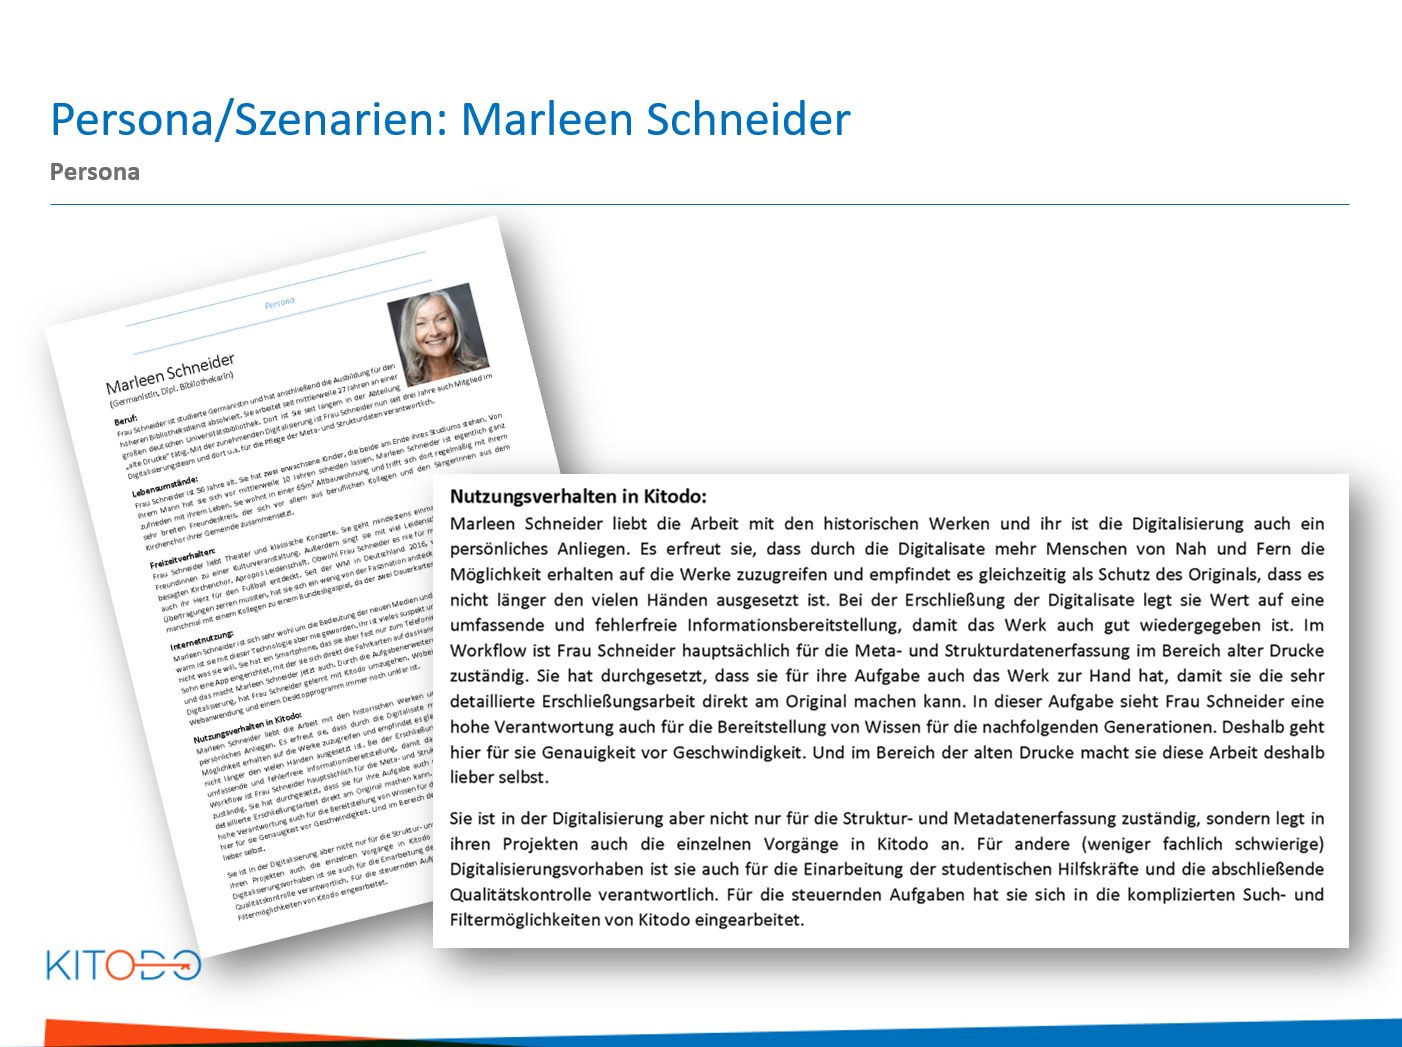
\includegraphics[width=0.9\textwidth,height=\textheight]{media/persona.png}

}

\caption{\label{fig-persona}Bild einer Personabeschreibung}

\end{figure}%

Außerdem kann es sich lohnen, solche Use Cases zu visualisieren. Dabei
können Start, Ende, mögliche Verzweigungen, alternative Aktionen und
mehr mit verschiedenen Formen modelliert werden. Dafür können
formalisierte Systeme wie die Unified Modelling Language (UML) zum
Einsatz kommen. Sie bietet ein Set verschiedener Formen, um Start, Ende,
Verzweigungen, Alternativen und mehr visuell zu beschreiben. Aber auch
Skizzen können Nutzungsszenarien bereits verdeutlichen und als
Diskussionsgrundlage dienen, z.\,B.~in Form von Storyboards, die in
einem eigenen \hyperref[storyboards-als-fruxfche-methode]{Unterkapitel
zu dieser Methode} noch beschrieben werden.

Use Cases können sowohl als Grundlage für den Entwicklungsprozess dienen
als auch für die Evaluation eines Systems (siehe Abschnitt
\hyperref[evaluierung]{„Evaluierung``}). Für die Nutzenden-Personas
einer Bibliothek kann eine breite Palette von Use Cases existieren.
Manche sind dabei eher allgemein zu verstehen, andere
bibliotheksspezifisch und natürlich sind alle je nach Einrichtung bzw.
Anforderungen beliebig erweiterbar. Zu beachten ist, dass sowohl
Personas als auch Use Cases zwingend auf der Grundlage
vertrauenswürdiger Daten wie denen aus der Bedarfsermittlung erstellt
werden sollten. Solche Methoden ohne Kenntnisse der Zielgruppen
anzuwenden kann nur zur Reproduktion der eigenen Meinung führen.

\subsection{Methoden}\label{sec-methoden}

Testaufgaben für Usability-Tests werden erstellt, um typische
Nutzungsszenarien mit Hinblick auf die Usability des Systems hin zu
überprüfen. Die folgenden Methoden können relativ einfach umgesetzt
werden, generieren jedoch bereits wertvolle Erkenntnisse.

\subsubsection{Think-Aloud-Methode}\label{think-aloud-methode}

Die zentrale Idee der Think-Aloud-Methode ist, dass Proband*innen
während der Interaktion mit dem zu evaluierenden System ihre Meinungen,
Gedanken und Gefühle laut aussprechen.

Dadurch wird es den Beobachter*innen ermöglicht, zuvor unsichtbare,
kognitive Prozesse der Proband*innen zu beobachten sowie einen Einblick
in typische Nutzungsweisen zu gewinnen. Durch die Verbalisierung und
Beschreibung des Systems durch die Nutzenden lernt man zeitgleich die
Nutzer*innenterminologie für bestimmte Sachverhalte kennen, die teils
erheblich von der Fachsprache abweichen wird. Die Ergebnisse der Methode
können z.\,B.~durch Notizen oder Audioaufnahmen festgehalten werden.

\subsubsection{Co-Discovery Learning}\label{co-discovery-learning}

Die Kernherausforderung bei der Erstellung von Think-Aloud-Protokollen
ist es, die Proband*innen kontinuierlich zu motivieren, selbst kleinste
Gedanken zu verbalisieren. Beim Co-Discovery Learning arbeiten zwei
Testpersonen gleichzeitig an einem System und helfen sich gegenseitig
bei der Erfüllung der Aufgaben. Dadurch entstehen Gespräche und
gewissermaßen automatisch ein Think-Aloud-Protokoll beider Personen.

Die Methode bildet einerseits eine realistische Arbeitssituation des
gegenseitigen Helfens ab und normalisiert andererseits das laute
Aussprechen von Gedanken innerhalb einer Dialogsituation.

\subsubsection{Quantitative Methoden}\label{quantitative-methoden}

Beobachtungsmethoden generieren primär qualitative Daten, ebenso wie
viele Inspektionsmethoden. Aus Managementsicht werden jedoch oft
Entscheidungen auf Grundlage von quantitativen Daten bevorzugt, da diese
häufiger als Fakten wahrgenommen werden.

Einfache, relativ leicht zu erhebende quantitative Metriken im Rahmen
von Usability-Tests sind z.\,B.:

\begin{itemize}
\item
  Nutzungsfehler pro Zeiteinheit,
\item
  Anzahl nicht benötigter Befehle (Menüs, Icons, Links),
\item
  benötigte Zeit für den Abschluss einer Arbeitsaufgabe (insbesondere im
  Vergleich mit einer vorherigen Iteration),
\item
  benötigte Anzahl an Klicks/Links, um an ein bestimmtes Ziel zu kommen.
\end{itemize}

Der „Benutzungsfragebogen ISONORM 9241/10`` bietet einen interessanten
Kompromiss zwischen qualitativen und quantitativen Daten, da er
qualitative Aussagen bezüglich der Usability eines Systems (z.\,B.
Aufgabenangemessenheit und Selbstbeschreibungsfähigkeit) mithilfe einer
siebenstufigen Likert-Skala abbildet. Der
\href{https://people.f3.htw-berlin.de/Professoren/Pruemper/instrumente.html}{Fragebogen}
ist frei im Internet verfügbar. Beachtet werden muss, dass für
belastbare quantitative Daten die Größe der Testgruppe deutlich steigen
muss, um Verfälschungen durch Einzelpersonen zu vermeiden.

\subsection{Einbeziehung von Nutzenden in die
Entwicklung}\label{einbeziehung-von-nutzenden-in-die-entwicklung}

Als Grundlage für Personas oder Use Cases und alle weiteren Schritte ist
die Einbeziehung von tatsächlichen Nutzenden in die Entwicklung also
bereits in einem frühen Stadium möglich und sinnvoll. Diese Einbeziehung
sichert ab, dass wesentliche Ziele der Nutzenden erreicht werden und in
mitunter komplexen Entwicklungsprozessen die richtigen Schwerpunkte
gesetzt werden. Dafür stehen verschiedene Methoden zur Verfügung.

Nachfolgend werden drei Ansätze vorgestellt:

\begin{itemize}
\item
  Storyboards~-- Skizzierung von Interaktionskonzepten
\item
  Wireframes und Mock-Ups~-- Skizzen der Oberflächen
\item
  Prototypen~-- erste funktionsfähige Iterationen
\end{itemize}

\subsubsection{Storyboards als frühe
Methode}\label{storyboards-als-fruxfche-methode}

Ein Storyboard illustriert, wie ein User Interface (UI,
Nutzer*innenoberfläche) auf Eingaben reagiert, ohne das Interface
visuell perfekt darzustellen. Es kann genutzt werden, um in Use Cases
bestimmte Aktionen zu illustrieren.

Die Visualisierung von Interaktionsideen kann Beteiligten helfen,
mögliche Abläufe nachzuvollziehen. Storyboards sind dabei oft leichter
verständlich als z.\,B.~technische Diagramme mit der oben genannten UML.
Trotzdem ist darauf zu achten, dass Ideen und Konzepte für Stakeholder
und Nutzende klar beschrieben werden, um Missverständnisse zu vermeiden.
In dieser Form lassen sich Storyboards nutzen, um z.\,B.~verbale
Beschreibungen oder Nutzungsszenarien zu ergänzen.

Durch die noch vage Darstellung der Idee können dann Diskussionen
angeregt werden. Beispielsweise können Storyboards in Fokusgruppen
vorgestellt und diskutiert oder auch in Einzelgesprächen mit
verschiedenen Stakeholdern analysiert werden. Möglichst alle Fragen und
Ideen sollten dabei ohne Limitierungen behandelt werden können und die
Ergebnisse festgehalten werden.

Vor- und Nachteile von Storyboards im Überblick:

\begin{longtable}[]{@{}
  >{\raggedright\arraybackslash}p{(\columnwidth - 2\tabcolsep) * \real{0.4865}}
  >{\raggedright\arraybackslash}p{(\columnwidth - 2\tabcolsep) * \real{0.4865}}@{}}
\toprule\noalign{}
\begin{minipage}[b]{\linewidth}\raggedright
Vorteile
\end{minipage} & \begin{minipage}[b]{\linewidth}\raggedright
Nachteile
\end{minipage} \\
\midrule\noalign{}
\endhead
\bottomrule\noalign{}
\endlastfoot
leicht verständlich, für alle Stakeholder geeignet & nicht jeder Use
Case oder jede Interaktionsmöglichkeit ist darstellbar \\
bereits im frühen Entwurfsprozess einsetzbar & digitale, nichtlineare
Produkte (z.\,B.~Websites) sind schwer darstellbar \\
schnelle Erstellung ohne Vorkenntnisse möglich & ggf.~Unklarheiten bei
der Nutzung (z.\,B.~durch unklare Symbole) \\
\end{longtable}

\subsubsection{Wireframes und Mock-Ups}\label{wireframes-und-mock-ups}

Wireframes und Mock-Ups sind Prototypen und werden vor allem dazu
genutzt, erste Skizzen für Struktur, Layout und Funktionalitäten eines
Interface vorzustellen. Ähnlich wie Storyboards dienen sie als einfach
zu erstellende Diskussionsgrundlage, mit deren Hilfe ein Abgleich der
Vorstellungen von einem System und der Gestaltungsmöglichkeiten
durchgeführt werden kann.

\begin{figure}

\centering{

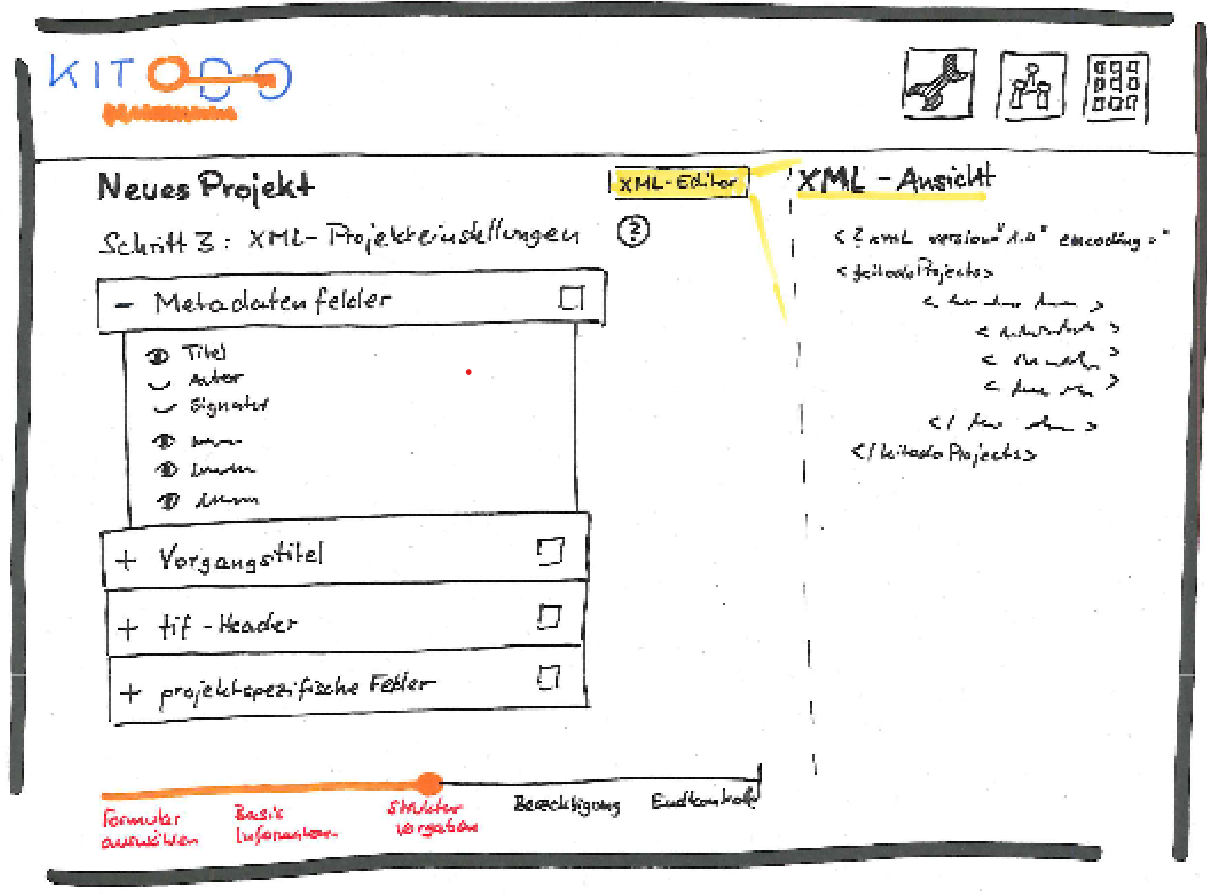
\includegraphics[width=0.45\textwidth,height=\textheight]{media/wireframe.png}

}

\caption{\label{fig-wireframe}Bild eines Papierprototypen für den
Relaunch des Digitalisierungssystems Kitodo}

\end{figure}%

Ein Wireframe („Drahtmodell``) ist eine noch undetaillierte
(„low-level``) Ausarbeitung eines Interfaces, vor allem darauf
ausgerichtet, die Positionierung der einzelnen Elemente zu planen. Daher
sind z.\,B.~Bilder oder Buttons als Kästchen dargestellt und Texte als
Striche und ähnliches (siehe Abbildung~\ref{fig-wireframe}). Ein Mock-Up
ist, im Kontext Design, eine ausgereifte („high-level``) Version des
Interfaces mit realistischen Farben, Schriftarten und Elementen. Sowohl
Wireframes als auch Mock-Ups sind also rein statische Entwürfe des
zukünftigen Produkts im Gegensatz zu interaktiven Prototypen, die echte
Funktionalitäten enthalten.

\subsubsection{Prototypen}\label{prototypen}

Interaktive Prototypen besitzen als nächsthöhere Form eines geplanten
Produkts bereits erste Funktionen des geplanten Interfaces. Auch hier
gibt es eine Spanne von rudimentären, low-level bis hin zu ausgereiften,
high-level Prototypen, die durch Iterationen schrittweise erreicht
werden. Üblich ist außerdem die Unterteilung in „vertical slice``, die
qualitativ hochwertige Umsetzung nur eines bestimmten Teils des
Produkts, und „horizontal slice``, die prototypische Umsetzung einer
möglichst großen Bandbreite des späteren Systems.

Erste Prototypen müssen dabei noch nicht zwingend programmiert werden,
sondern können durch entsprechende Prototyping-Software, wie
\href{https://www.figma.com}{Figma} oder
\href{https://www.axure.com}{Axure}, umgesetzt werden. Diese besitzen
eine Art Bausystem für Interfaces mit mehreren Ansichten, die über
Aktionen wie den Klick auf einen Button verbunden werden können. So kann
Nutzenden gewissermaßen ein Produkt vorgetäuscht werden, das dann mit
rudimentären Funktionen bereits getestet werden kann.

Während des eigentlichen Entwicklungsprozesses wird der anfängliche
Prototyp mit jeder Iteration hochwertiger und nimmt mehr den Charakter
eines vollen Systems an. Es empfiehlt sich, nach Iterationen regelmäßig
zu evaluieren, ob neue Funktionen oder Änderungen noch für die
Zielgruppen geeignet sind.

\subsection{Evaluierung}\label{evaluierung}

Die vorangegangenen Abschnitte haben herausgestellt, wie wichtig es ist,
regelmäßig Feedback der Nutzenden zu erhalten. Eine zentrale Datenquelle
dafür ist die Begleitung eines Projekts durch Evaluierungen. Ein
Beispiel für eine lebendige Evaluierungskultur ist das
``\href{https://uxanddiscovery.library.harvard.edu/}{User Research
Center'' der Harvard Library}, das regelmäßig verschiedene Methoden
anwendet, um Angebote gemeinsam mit Nutzenden zu evaluieren und diese
öffentlich auf der Homepage teilt.

Im Rahmen der Usability-Evaluierung entscheidet man dabei grob zwei
Methoden: Beobachtungstest und Inspektionstests
(Abbildung~\ref{fig-usux}). Während erstgenannte unter Einbeziehung von
Nutzer*innen durchgeführt werden, werden Inspektionstests häufig durch
Usability-Expert*innen realisiert.

Als Vorteil der Beobachtungstests erweist sich aus der Praxissicht, dass
diese auch ohne eine formale Usability-Ausbildung durch engagierte
Mitarbeiter*innen durchgeführt werden können. Im Folgenden soll deshalb
das prinzipielle Vorgehen bei einem Beobachtungstest skizziert werden.

\subsubsection{Testgruppen}\label{testgruppen}

Die Testgruppe muss die potentielle Nutzungsgruppe bestmöglich
repräsentieren, jedoch nicht sehr groß sein. Die Erfahrung zeigt, dass
ca.~fünf Testpersonen ausreichen, um die wichtigsten Usabilityprobleme
eines Systems zu identifizieren, siehe Jakob Nielsen (2000). Statt eines
einzigen Tests mit vielen Teilnehmenden bieten sich daher schnell
durchzuführende Tests mit wenigen Teilnehmenden an, um ein Produkt
iterativ zu verbessern. Möchte man jedoch verschiedene Typen von
Nutzer*innen analysieren oder quantitative Ergebnisse sammeln, muss die
Gruppengröße entsprechend wachsen.

Neben den typischen Streuungsmerkmalen wie demographischen und
kulturellen Faktoren (z.\,B.~Bildungshintergrund) bietet es sich an,
Nutzer*innen auszuwählen, die über ein unterschiedliches Maß an
Vorwissen über das zu entwickelnde oder verwandte Produkte verfügen.
Außerdem sollten Personen integriert werden, welche von Einschränkungen
betroffen sind, die im Abschnitt
\hyperref[accessibility]{„Barrierefreiheit``} thematisiert wurden.

\subsubsection{Testablauf und
Vorbereitungen}\label{testablauf-und-vorbereitungen}

Nach der Rekrutierung repräsentativer Nutzer*innen und der Vorbereitung
der benötigten Materialien und der Testumgebung bietet sich ein
Pilottest mit Proband*innen an. Dieser dient der Validierung der eigenen
Annahmen über die Testaufgaben (s.\,u.) und die Machbarkeit des Ablaufs.

Die Testumgebung sollte eine entspannte und natürliche Arbeitsumgebung
vermitteln. Diese ist in jedem Fall einer künstlichen Laborumgebung
vorzuziehen. Während der Beobachtungstests ist sicherzustellen, dass
keine Unterbrechungen, z.\,B.~in Form von Telefonanrufen, erfolgen,
damit die Proband*innen das zu evaluierende System konzentriert testen
können.

Nach dem Beobachtungstest sollte es den Proband*innen ermöglicht werden,
die Testergebnisse zu erhalten. Außerdem ist es neben dem
obligatorischen Dank für die Teilnahme üblich, eine Aufmerksamkeit~-- je
nach Dauer z.\,B.~Kaffee, Süßes, Gutscheine~-- auszuhändigen, um die
eigene Wertschätzung für das zeitliche Investment der Proband*innen
auszudrücken. In einer Erklärung zum Datenschutz ist die anonyme
Datennutzung zuzusichern.

\subsubsection{Testaufgaben}\label{testaufgaben}

Wie die Testgruppen müssen auch die Testaufgaben repräsentativ für den
späteren Einsatzzweck des Systems sein. Die von den Proband*innen zu
bearbeitenden Testaufgaben müssen realistische Aufgaben in bzw.~mit dem
System sein und in der gegebenen Zeit absolvierbar sein. Dabei ist zu
beachten, dass sich die Arbeitsaufgaben an tatsächlichen Use Cases
orientieren und nicht trivial sind.

Die Formulierung der Arbeitsaufgaben muss unmissverständlich für die
Proband*innen sein und auf deren (mitunter variierendes) Vorwissen
eingehen. Ein Pilottest hilft, dies zu überprüfen.

Die Gestaltung der einzelnen Aufgaben sollte einer Dramaturgie folgen,
um die Proband*innen während des gesamten Tests zu motivieren. Das heißt
konkret, dass die ersten Teilaufgaben leicht zu lösen sein sollten und
deren Schwierigkeit dann kontinuierlich zunimmt, um durch komplexere
Aufgaben belastbare Aussagen zu erhalten.

\section{Zusammenfassung und
Ausblick}\label{zusammenfassung-und-ausblick-2}

Es gibt verschiedenste Methoden mit denen Bedarfe ermittelt und Nutzende
in die Entwicklung von digitalen Diensten einbezogen werden können~-- je
nach Umfang des Produkts und des Anwender*innenkreises. Usertests
erfordern ein anderes Zeitmanagement als die Entwicklung von Personas.
Auch der Anwendungsfall nimmt Einfluss auf die Methodenauswahl. So kann
für die Entwicklung eines neuen Designs die Verwendung von Wireframes
und Mockups bei der Bedarfsermittlung hilfreich sein. Wird ein Portal
mit neuen Interaktionsmöglichkeiten entwickelt, empfehlen sich
Prototypen, mit denen auch die Interaktionen getestet werden können.

\bookmarksetup{startatroot}

\chapter{Datenschutz \& Sicherheit}\label{sec-sicherheit}

\begin{tcolorbox}[enhanced jigsaw, leftrule=.75mm, toprule=.15mm, left=2mm, opacityback=0, arc=.35mm, colback=white, breakable, colframe=quarto-callout-note-color-frame, rightrule=.15mm, bottomrule=.15mm]
\begin{minipage}[t]{5.5mm}
\textcolor{quarto-callout-note-color}{\faInfo}
\end{minipage}%
\begin{minipage}[t]{\textwidth - 5.5mm}

\vspace{-3mm}\textbf{Zusammenfassung}\vspace{3mm}

Dieses Kapitel soll für die Themen IT-Sicherheit und Datenschutz
sensibilisieren und geht dabei auch auf bibliotheksspezifische
Besonderheiten ein. Im Bereich \hyperref[datenschutz]{Datenschutz}
müssen insbesondere beim \hyperref[sec-datenschutz-externe]{Einsatz
externer Anbieter} besondere Vorkehrungen getroffen werden. Im Bereich
der \hyperref[it-sicherheit]{IT-Sicherheit} werden mögliche
\hyperref[sec-sicherheitsvorfall]{Sicherheitsvorfälle} beschrieben,
\hyperref[pruxe4ventivmauxdfnahmen]{Präventivmaßnahmen} vorgestellt und
\hyperref[handlungsempfehlungen]{Handlungsempfehlungen} gegeben.

\end{minipage}%
\end{tcolorbox}

\section{Einleitung}\label{einleitung-4}

In den letzten Jahren ist die Zahl der Angriffe auf
Bildungseinrichtungen, insbesondere Hochschulen und ihre Bibliotheken,
deutlich gestiegen. Laut der Hochschulrektorenkonferenz (HRK) waren bis
Januar 2023 insgesamt 24 Hochschulen bzw.~Universitäten solchen
cyberkriminellen Angriffen ausgesetzt und nahmen Schaden (MDR 2023).
Informationseinrichtungen aller Sparten werden zudem mit sicherheits-
und datenschutzrelevanten Aufgaben konfrontiert.

Die Entwicklung hin zur Digitalisierung, Automatisierung und
Virtualisierung zieht nicht nur die Technisierung eigener Geschäftsgänge
und Dienstleistungen nach sich. Diese Entwicklung erfordert auch eine
größere Sensibilität und Aufmerksamkeit hinsichtlich der Sicherheit der
eigenen Systeme. Safety und Security sind hierfür wichtige, zu
unterscheidende Grundprinzipien.

\begin{tcolorbox}[enhanced jigsaw, leftrule=.75mm, toprule=.15mm, left=2mm, opacityback=0, arc=.35mm, colback=white, breakable, colframe=quarto-callout-important-color-frame, rightrule=.15mm, bottomrule=.15mm]
\begin{minipage}[t]{5.5mm}
\textcolor{quarto-callout-important-color}{\faExclamation}
\end{minipage}%
\begin{minipage}[t]{\textwidth - 5.5mm}

\textbf{Security} beinhaltet alle Maßnahmen zum Schutz vor Diebstahl
oder Beschädigung von Soft- und Hardware. \textbf{Safety} meint den
sicherheitsbewussten Umgang mit Netzwerken und Daten.

\end{minipage}%
\end{tcolorbox}

Darüber hinaus nimmt die Bedeutung des
\hyperref[datenschutz]{\textbf{Datenschutzes}} weiter zu. Die
Verarbeitung von schützenswerten personenbezogenen Daten wird evtl.
nicht nur in der Bibliothek oder übergeordneten Einrichtung selbst
vorgenommen, sondern zunehmend von externen Dritten, wie
bspw.~Cloud-Infrastrukturen. Umso bedeutender wird im Hinblick auf die
Sicherheit die Datensparsamkeit und das Bewusstsein, welche
personenbezogenen Daten in welchen Systemen verarbeitet werden sollen
oder müssen.

Bibliotheken verstehen sich als Orte, die ihre Informationen und
vielschichtigen Dienstleistungen i.\,d.\,R.~einer großen Nutzendenschaft
zur Verfügung stellen. Sie tragen durch ihre Arbeit zur Umsetzung der
Openness-Strategie in Gesellschaft und Wissenschaft bei. Offenheit und
Transparenz sind schützenswerte Haltungen von Bibliotheken, welche
gleichzeitig aber auch eine größere Angriffsfläche ermöglichen.

Doch was macht Bibliotheken und Hochschulen so interessant für Angriffe?
An diesen Orten werden für Cyberkriminelle interessante Daten verwaltet.
Dazu gehören personenbezogene Daten von Nutzenden und Beschäftigten,
schützenswerte Forschungsdaten, Bewegungsdaten, Lizenzdaten, Daten zur
Nutzung von Literatur, etc. Die dabei abgegriffenen Daten können
u.\,a.~für Identitätsdiebstahl, Offenlegung privater Informationen oder
für die Erstellung eines detaillierten Nutzerprofils herangezogen werden
(Holländer 2023).

IT-Sicherheit und Datenschutz sind auch immer eine Frage der
Zuständigkeit. Je nach Größe, Art und Organisationsstruktur der
Bibliothek muss die IT-Sicherheit mit den beteiligten Instanzen wie
Stadtverwaltung, Verbundzentrale, den Rechen- und IT-Zentren der
Institution und den IT-Sicherheitsbeauftragten und
Datenschutzbeauftragten in Bezug auf die Verantwortlichkeiten abgestimmt
werden. Grundsätzlich liegt die Aufgabe der Sensibilisierung und
Schulung des Bibliothekspersonals im direkten Verantwortungsbereich der
Bibliothek.

\begin{figure}[t]

\centering{

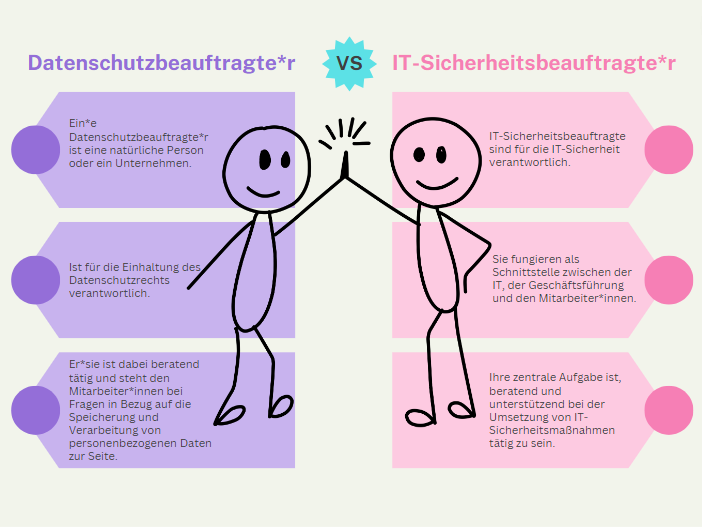
\includegraphics{media/datenschutz-vs-sicherheits-beauftragte.png}

}

\caption{\label{fig-datenschutz-datensicherheit}Abgrenzung
Datenschutzbeauftragte*r IT-Sicherheitsbeauftrage*r}

\end{figure}%

Wenig ist zum Thema IT-Sicherheit in Bibliotheken veröffentlicht worden
(Kost u.~a. 2022). Deshalb soll dieses Kapitel zur Vorbeugung nicht nur
für das Thema IT-Sicherheit sensibilisieren, eine Beschreibung eines
Sicherheitsvorfalls und einen Überblick über die Richtlinien und
Vorgaben geben, sondern auch für Präventivmaßnahmen werben und
Handlungsempfehlungen geben. Gleiches gilt für den Datenschutz.

\section{Datenschutz}\label{datenschutz}

Innerhalb der EU gilt seit 2018 die Datenschutz-Grundverordnung
(\href{https://www.bmwk.de/Redaktion/DE/Artikel/Digitale-Welt/europaeische-datenschutzgrundverordnung.html}{DSGVO}),
nach der personenbezogene Daten grundsätzlich zu schützen sind. Sie
regelt unter anderem, dass jede Person das Recht auf Schutz der sie
betreffenden personenbezogenen Daten hat. So dürfen Daten nur für einen
bestimmten Zweck erhoben (Zweckbindung) und auch nicht für andere

Vorhaben weiterverarbeitet werden (gem. Art.~5 II DSGVO). Ferner wird in
Art.~37 DSGVO die Ernennung eines Datenschutzbeauftragten geregelt.

Ergänzt wird diese Grundverordnung durch die einzelnen nationalen
gesetzgebenden Instanzen. In Deutschland geschieht dies sowohl auf
Bundes- als auch auf Landesebene, in Form des Bundesdatenschutzgesetzes
(BDSG) sowie der 16 Landesdatenschutzgesetze.

In Österreich wird die DSGVO ergänzt durch das Datenschutzgesetz (DSG)
und das Netz- und Informationssystemsicherheitsgesetz (NISG).

Ähnliche Gesetze wurden auch außerhalb der EU erlassen. So trat Anfang
September 2023 in der Schweiz die neue Verordnung über
Datenschutz-zertifizierungen (VDSZ) in Kraft, welche sich an den
Grundzügen der DSGVO orientiert.

Aufgrund der stetigen Weiterentwicklung von Software und neuen
Technologien hat die Europäische Kommission einen Vorschlag für ein
neues Gesetz zur Widerstandsfähigkeit von Cyberangriffen, den
\href{https://digital-strategy.ec.europa.eu/en/policies/cyber-resilience-act}{Cyber
Resilience Act}, auf den Weg gebracht. Gemäß diesem Vorschlag sollen
Verbraucher*innen und Unternehmen beim Kauf von Produkten und Software
mit digitalen Komponenten geschützt werden, indem verbindliche
Cyber-Sicherheits-Anforderungen für diese Leistungen durch die
Hersteller eingeführt werden sollen. Im nächsten Schritt werden nun das
Europäische Parlament und der Europäische Rat über diesen Vorschlag
beraten.

Um den Schutz personenbezogener Daten gewährleisten zu können, gibt es
verschiedene Ansätze:

\begin{itemize}
\item
  \textbf{Verschlüsselung}: Daten werden auf verschlüsselten Servern
  gespeichert, ebenso ist die Übertragung Ende-zu-Ende verschlüsselt
\item
  \textbf{Separierung}: Personendaten werden getrennt von
  nicht-sensiblen Daten gehalten (siehe
  \hyperref[identity-management]{IDM})
\item
  \textbf{Pseudonymisierung}: Nutzer*innen-Daten werden mit Pseudonymen
  präpariert, sodass sie nicht mehr oder nur unter großem Aufwand den
  einzelnen Personen zuzuordnen sind
\item
  \textbf{Anonymisierung}: Daten werden derart verändert, dass sie nicht
  rückverfolgbar sind (z.\,B.~Maskierung IP-Adressen)
\end{itemize}

Die Pseudonymisierung und Anonymisierung kann auch im Laufe der Erhebung
der personenbezogenen Daten zur Anwendung kommen, sofern bestimmte Daten
nicht mehr für einen konkreten Zweck erforderlich sind.

Leider sind personenbezogene Daten für Bibliotheksstatistiken oft
notwendig (siehe \hyperref[kosten]{Kosten}). In diesem Fall sollten
ebenfalls pseudonymisierte oder anonymisierte Datensätze zur Grundlage
genommen werden.

Für alle personenbezogenen und personenbeziehbaren Daten sind Lösch-
oder Anonymisierungsfristen festzulegen. Die Anonymisierungsfristen
ergeben sich aus den Vorgaben der DSGVO und müssen betrieblichen und
rechtlichen Aspekten genügen. So ergeben sich Fristen für die
Speicherung von Daten über Gebühren (Entstehung, Bezahlung, \ldots) aus
den Landeshaushaltsordnungen oder anderen für die Einrichtung
maßgeblichen Regelungen. Betriebliche Gründe für die Länge von
Speicherfristen von personenbezogenen und personenbeziehbaren Daten
können sich aus Fristen für Einsprüche ergeben.

\subsection{Einsatz externer Anbieter}\label{sec-datenschutz-externe}

Für Software, die durch einen externen Anbieter gehostet wird
(Kapitel~\ref{sec-betriebsmodelle}), muss Folgendes sichergestellt sein:

\begin{itemize}
\item
  die Verschlüsselung der Datenübertragung
  (Ende-zu-Ende-Verschlüsselung)
\item
  Betrieb und Steuerung der Server innerhalb der EU
  (\href{https://de.wikipedia.org/wiki/Datenschutz-Grundverordnung}{DSGVO})
\item
  der Ausschluss von User-Tracking durch Ad-Tech (Werbenetzwerke)
\item
  der Abschluss eines
  \href{https://de.wikipedia.org/wiki/Datenverarbeitung_im_Auftrag}{Datenverarbeitungsvertrags
  im Auftrag}
\end{itemize}

Die über die vergangenen Jahrzehnte geschehenen sukzessiven Aufkäufe
kleinerer Softwareanbieter durch einige wenige große kommerzielle
Bibliotheksdienstleister hat ganze Firmenkonglomerate entstehen lassen,
die inzwischen den Bibliotheksmarkt dominieren. Einige von ihnen, die
Dienste für wissenschaftliche Bibliotheken anbieten, wandeln sich in den
letzten Jahren zu Data-Analytics-Konzernen. In diesem Zuge präparieren
sie ihre cloudbasierten Lösungen mit Trackern, die Verhaltensprofile
über die Nutzer*innen erstellen. Durch die ebenfalls seitens der
Anbieter gestellten Zugangsauthentifizierungssysteme wird versucht,
zusätzlich eine möglichst hohe Personalisierung bei der Erstellung
einzelner Profile zu erreichen. Die dabei entstehenden Datenflüsse
werden für gewöhnlich nicht transparent gemacht (Siems 2022). Der
Einsatz solcher Analytics-Technologien unterminiert die Integrität
konventioneller IDM-Systeme und tangiert somit nicht nur
datenschutzrechtliche Belange, sondern auch die IT-Sicherheit.
Idealerweise sollte bereits vor der Anschaffung einer Sofwarelösung
abgeklärt werden, ob solche Analytics-Technologien eingesetzt werden. Im
Zweifelsfall sollte immer der*die lokale Datenschutzbeauftragte oder
IT-Sicherheitsbeauftragte hinzugezogen werden.

In ihrer besonderen Rolle als Institutionen für Informationsversorgung
und Bereitstellung von Wissensinfrastruktur greifen Bibliotheken auch
auf die Dienste externer Anbieter zurück, z.\,B.~durch Verträge mit
Wissenschaftsverlagen über digitale Literaturangebote. Hierbei ist es
wichtig, dass Bibliotheken in diesen Verträgen darauf bestehen, dass das
Tracking des Nutzungsverhaltens der Forschenden ausgeschlossen wird
(Reda (2022)), um die Wissenschaftsfreiheit und die informationelle
Selbstbestimmung zu schützen (DFG 2021).

\section{IT-Sicherheit}\label{it-sicherheit}

Der Begriff IT-Sicherheit bezeichnet den Schutz von IT-Systemen~-- das
heißt von Computern, Netzwerken, digitalen Geräten und den darauf
verarbeiteten Daten~-- vor unbefugtem Zugriff, Manipulation, Verlust,
Zerstörung oder anderen Bedrohungen. Sowohl technische als auch
organisatorische Maßnahmen sind ein zentraler Bestandteil des Schutzes
digitaler Infrastrukturen.

Auf nationaler Ebene liegt die Zuständigkeit unter anderem beim
Bundesamt für Sicherheit in der Informationstechnik
(\href{https://www.bsi.bund.de/DE/Das-BSI/Auftrag/auftrag_node.html}{BSI}),
welches seit 1991 mit der Aufgabe betraut ist, das Regierungsnetz und
die kritischen Infrastrukturen (KRITIS) zu schützen. Auf Bundesebene
wurde es eine zentrale Anlaufstelle für Sicherheitsstandards, sowie
Meldestelle bei IT-Krisen. Es stellt unterschiedliche Normen zur
IT-Sicherung zur Verfügung. Wann welcher Standard greift, hängt von der
Komplexität des Einzelfalls ab.

Für Bibliotheken sind hierbei auch die „Checklisten zum
\href{https://www.bsi.bund.de/DE/Themen/Unternehmen-und-Organisationen/Standards-und-Zertifizierung/IT-Grundschutz/IT-Grundschutz-Kompendium/it-grundschutz-kompendium_node.html}{IT-Grundschutz-Kompendium}``
nach dem BSI-Standard 200-2 sehr empfehlenswert, da in diesen der
aktuelle Stand der Integration des Grundschutzes überprüft werden kann.
In diesem Zusammenhang wird auch auf die ISO/IEC-27000-Familie
hingewiesen. In dieser Normenreihe sind neben definierten und stets
aktuell gehaltenen Standards, die Anforderungen an Information Security
Management Systems (ISMS), Empfehlungen für Kontrollmechanismen, als
auch Best-Practices-Empfehlungen zu Aufbau und Organisation von
Informationsfreiheit enthalten.

\subsection{Sicherheitsvorfall}\label{sec-sicherheitsvorfall}

Prominente Vorfälle in verschiedenen wissenschaftlichen Einrichtungen
haben in den letzten Jahren Schwachstellen in IT-Systemen offenbart, die
ernstzunehmende Sicherheitslücken darstellen. Dabei ist zu beachten,
dass sowohl Maschinen als auch Menschen verantwortlich für diese Lücken
sein können.

\subsubsection{Angriffsmethoden}\label{angriffsmethoden}

Folgende sind die häufigsten Angriffsmethoden:

\begin{itemize}
\item
  \textbf{Social Engineering:} Unter Social Engineering versteht man
  Methoden, die zum Vertrauensgewinn eingesetzt werden, um anschließend
  an sensible Informationen, Zugangsdaten für Systeme oder finanzielle
  Mittel zu gelangen. Social Engineering-Attacken können über
  persönliche Kontakte oder über Webdienste wie E-Mails oder Webseiten
  durchgeführt werden.
\item
  \textbf{Phishing:} Hierbei werden seriös wirkende E-Mails versendet,
  um den Empfänger*innen Kennwörter oder Zahlungsinformationen zu
  entlocken, um so an sensible Daten zu gelangen. Die „Qualität``
  derartiger gefälschter E-Mails variiert stark. Es zeigt sich jedoch,
  dass sie kontinuierlich professioneller umgesetzt werden und
  schwieriger zu identifizieren sind. Häufig werden Phishing-Attacken
  mit Links auf präparierte Webseiten (sog. Watering Holes) kombiniert.
  In diesem Fall dienen sie auch als Haupteintrittstore für Malware.
\item
  \textbf{Malware}: Alle Arten von Schadsoftware, die auf dem
  Zielrechner ausgeführt wird, um z.\,B.~Daten auszuspionieren, das
  normale Systemverhalten zu unterbrechen oder Schäden zu verursachen.
  Typische Beispiele sind Ransomware, Viren oder Würmer.
\item
  \textbf{Ransomware:} Bei dieser Art des Angriffs wird der Zugriff auf
  Daten eingeschränkt oder unterbunden, z.\,B.~durch Verschlüsselung.
  Für die Wiederherstellung des Zugriffs wird ein Lösegeld gefordert.
  Ransomware hat von allen Angriffsmethoden das größte
  Schadenspotential. Neben Lösegeldforderungen entstehen hohe Ausfalls-
  und Wiederherstellungskosten.\\
  Als Beispiel: Für die direkten Kosten des Ransomware-Angriffs 2019 auf
  die JLU Gießen werden mit Stand 2023 ca.~1,7 Mio. € für
  Schadensanalyse und -behebung kalkuliert. Zusätzliche Kosten für
  Aufwände und Workarounds sind in dieser Analyse nicht berücksichtigt
  und lassen sich schwer beziffern (Kost u.~a. (2022)).
\item
  \textbf{Viren} und \textbf{Würmer:} Schadprogramme, die sich
  selbständig replizieren und/oder an andere Programme anhängen, um
  möglichst viele Rechner zu infizieren. Häufig dienen Viren und Würmer
  zur Verbreitung der eigentlichen Schadsoftware.
\item
  \textbf{Denial-of-Service-Attacken (DoS):} Ein Angriff, bei dem sehr
  viele gleichzeitige Anfragen an einen Server gestellt werden, um
  dessen Verfügbarkeit zu beeinträchtigen. Häufig kommen Distributed
  Denial-of-Service (DDoS) Angriffe vor, bei denen die Anfragen von
  vielen unterschiedlichen Systemen in einem koordinierten Einsatz
  gestellt werden.
\end{itemize}

\subsubsection{Auswirkungen}\label{auswirkungen}

Bisherige Erfahrungen zeigen die weitreichenden Auswirkungen eines
cyberkriminellen Angriffs auf Bibliotheken. In den meisten Fällen ist
jedoch nicht nur die Bibliothek alleine betroffen, sondern die gesamte
Hochschule, Kommune oder Forschungseinrichtung. Kommt es zu einem
Angriff, ist es meist notwendig, alle IT-Dienste herunterzufahren. Eine
Abschottung einzelner Dienste kann kaum vorgenommen werden. Man kann
sich dies als einen „harten Cut`` und ein Herunterfahren aller eigenen
Server und virtuellen Maschinen zur Eingrenzung des schadhaften
Fremdzugriffs vorstellen. Diese harte Maßnahme wird vorgenommen, da man
nicht abschätzen kann, wo es im System schon zu welchen Schäden gekommen
ist. Die Folgen: es funktioniert schlimmstenfalls NICHTS mehr. (W)LAN,
Netzlaufwerke, Identity-Management und Anmeldedienste, E-Mail-Dienste,
Terminverwaltungstools, Personal-Verwaltungssysteme,
Türschließmechanismen, Zeiterfassung, IP-Telefonie, Lüftungs- und
Beleuchtungssysteme, etc. Alle netzbetriebenen Dienste sind ggf.~für
mehrere Tage, Wochen oder sogar Monate außer Betrieb.

Im Ernstfall können die vorhandenen Dienstgeräte und
Kommunikationsdienste nicht mehr verwendet werden. Aufgrund dessen kann
man zur Kommunikation auf private Geräte (Notebooks, Smartphones, etc.,
sofern die Mitarbeiter*innen bereit dazu sind) und alternative
E-Mail-Dienste ausweichen. Hier ist zu bedenken, dass diese
Adhoc-Lösungen nicht unbedingt den datenschutzrechtlichen Ansprüchen
entsprechen wenn kein Vertrag zur Auftragsdatenverarbeitung
abgeschlossen wird. Von besonderer Bedeutung ist in diesem Fall auch das
Identity Management System (IDMS), das nach einem Angriff gegebenenfalls
alternativ aufgebaut werden muss.

Die fortschreitende Digitalisierung, Automatisierung und Virtualisierung
kann durchaus auch hilfreich sein, wenn die Systeme nicht mehr
ausschließlich im eigenen Rechenzentrum betrieben werden. So können die
extern betriebenen Anwendungen ggfs. über alternative (mobile) Netzwerke
und mit bereits geprüften und wieder freigegebenen Notebooks schnell
wieder genutzt werden. Als Beispiel sei hier das
Bibliotheksmanagementsystem
(Kapitel~\ref{sec-bibliotheksmanagementsysteme}) genannt. Wenn dieses
bei einem Dienstleister gehostet wird, ist es in der Regel vom Angriff
nicht betroffen, sodass die Ausleihe und Rückgabe wieder zeitnah
ermöglicht werden können.

Zu guter Letzt darf auch nicht unterschätzt werden, welche zeitlichen
Ausmaße ein Angriff einnehmen kann und welche psychischen und sozialen
Auswirkungen er verursacht. Mitunter muss mit monatelangen
Einschränkungen gerechnet werden und es kann nicht davon ausgegangen
werden, dass alle Daten vollständig wiederhergestellt werden können.
Daher gilt es nicht nur, einen Angriff möglichst zu vermeiden, sondern
das Ausmaß möglicher Schäden zu minimieren.

\subsection{Präventivmaßnahmen}\label{pruxe4ventivmauxdfnahmen}

Um IT-Infrastruktur vor den zunehmenden Angriffen durch böswillige
Akteure (Hacking, Malware, Ransomware) abzusichern, können die folgenden
Empfehlungen als Grundlage dienen (Breeding, Marshall 2022):

\begin{itemize}
\item
  Die Infrastruktur herum sollte durch starke Sicherheitsvorkehrungen
  getragen werden.
\item
  Die Gefahr kurzfristig entstehender Sicherheitslücken sollte nicht
  unterschätzt werden.
\item
  Cloudbasierte Systeme sollten aktiv überwacht und der Überblick
  behalten werden.
\item
  Anbieter sollten aufgefordert werden, die Konzepte ihrer
  Sicherheitsvorkehrungen offenzulegen.
\item
  Gerade Administrator*innen sollten ihre Zugänge gesondert absichern.
\item
  Es sollte sichergestellt werden, dass jede Software stets auf dem
  aktuellen Stand ist, sowohl auf den Arbeitsplatz-PCs als auch den
  Servern.
\end{itemize}

\subsubsection{Passwortsicherheit}\label{passwortsicherheit}

Zu einem umfassenden IT-Sicherheitskonzept gehört, dass alle Beteiligten
einen bewussten Umgang mit Passwörtern praktizieren. Passwörter sollten
zum Beispiel nicht ohne Weiteres für Dritte zugänglich auf Papier oder
einem anderen Medium (z. B. unverschlüsselt auf dem Computer)
festgehalten werden. Bei Verdacht auf Angriff sollten alle betroffenen
Passwörter umgehend geändert werden. Bei einer großen Menge an
Passwörtern empfiehlt es sich, einen Passwort-Manager zu verwenden. Für
die Wahl des Passworts sollten die allgemein gültigen Empfehlungen
beachtet werden (beispielsweise die
\href{https://www.bsi.bund.de/DE/Themen/Verbraucherinnen-und-Verbraucher/Informationen-und-Empfehlungen/Cyber-Sicherheitsempfehlungen/Accountschutz/Sichere-Passwoerter-erstellen/sichere-passwoerter-erstellen_node.html}{Tipps
zu Erstellung sicherer Passwörter des BSI}).

\subsubsection{Authentifizierung und
Autorisierung}\label{authentifizierung-und-autorisierung}

Unter Authentifizierung verstehen wir grundsätzlich das eindeutige
Erkennen eines Zugriffs auf eine Ressource wie z.\,B.~einen Dienst oder
einen Computer, aber auch auf ein physisches Objekt wie z.\,B.~einen
Drucker.

In der Regel erfolgt heutzutage der Zugriff über ein Netzwerk, d. h.,
auch die Authentifizierung muss über das Netzwerk erfolgen. Für Geräte
(Computer) kann dies durch technische Merkmale wie den Media Access Code
(MAC Adresse) oder flexibler über die IP-Adresse durchgeführt werden.
Diese Merkmale authentifizieren jedoch nur das Gerät und lassen noch
keine Aussage darüber zu, wer dieses Gerät gerade benutzt.

Eine Authentifizierung einer Person erfolgt meistens über eine
eindeutige Kennung und ein zugehöriges Passwort. Wenn möglich, sollten
verschiedene Authentifizierungsverfahren miteinander kombiniert werden.
Es wird dann auch von einer 2-Faktor-Authentifizierung (2FA) bzw.~einer
Mehrfaktor-Authentifizierung (MFA) gesprochen.

Ist ein Zugriff eindeutig durch entsprechende Authentifizierung erkannt,
kann auf Basis verschiedener Informationen je nach Bedarf entschieden
werden, ob der Zugriff auch berechtigt ist. D. h., der Zugriff muss
autorisiert werden. Dies kann sehr individuell erfolgen (Konto A hat
Zugriff, Konto B nicht) oder anhand der Zugehörigkeit eines Kontos zu
einer bestimmten Personengruppe.

Alle Komponenten, die zur Authentifizierung und Autorisierung in einer
Einrichtung notwendig sind, werden auch als Authentifizierungs- und
Autorisierungsinfrastruktur (AAI) bezeichnet. Wurde in einer Einrichtung
eine AAI aufgebaut, auf welche jede Anwendung zurückgreifen kann, kann
man festlegen, dass nach einmaligem Login ein Zugriff auf alle
Anwendungen möglich und ein separates Einloggen nicht nötig ist. Dies
wird auch als \textbf{Single-Sign-On (SSO)} bezeichnet. Die möglichen
Verfahren sind in Abbildung~\ref{fig-sso} dargestellt: Benutzer*in
meldet sich auf einem \textbf{Portal} an und bekommt Zugriff auf alle
eingebundenen Dienste (links). Benutzer*in speichert alle Anmeldedaten
auf einem Datenträger oder im Netzwerk. Ein \textbf{lokal}es Programm
meldet ihn*sie separat bei jedem Dienst, Portal oder Ticketing-System
ein (Mitte). Benutzer*in meldet sich bei einem der Dienste an und
bekommt ein \textbf{Ticket} für den gesamten „Kreis der Vertrauten``
(rechts).

\begin{figure}

\centering{


\includegraphics{index_files/mediabag/media/sso-approaches.pdf}

}

\caption{\label{fig-sso}Herangehensweisen für Single-Sign-On}

\end{figure}%

Zentrale Komponenten sind hierbei der \textbf{Identity Provider (IDP)},
der auf Basis des dahinterliegenden IDMS eine digitale Identität
inkl.~notwendiger Benutzer*innenattribute bereitstellt und an dem die
einmalige Anmeldung stattfindet. Die genutzten Anwendungen werden
allgemein als \textbf{Service Provider (SP)} bezeichnet.

Eine gute Möglichkeit, das Internet sicher zu nutzen, ist das
\textbf{Virtual Private Network (VPN)}. Das VPN verschlüsselt die
Identität von Internetnutzer*innen. Damit wird es Dritten erschwert, die
Nutzer*innen im Internet zu verfolgen und Daten abzugreifen. VPN nutzt
dabei eine Echtzeitverschlüsselung. Informationen werden in eine
unleserliche Form umgewandelt und können nur mit einem Schlüssel wieder
in die ursprüngliche leserliche Form gebracht werden.

\subsubsection{Updates und Backups}\label{updates-und-backups}

Eine sichere Hard- und Software ist unabdingbar. Rechner sollten
ausreichend geschützt sein. Dazu gehören unter anderem aktuelle
Virenscanner und automatische Updates des Virenscanners, des
Betriebssystems und jeder auf dem Rechner laufenden Software. Fehlende
Updates können als Einfallstore genutzt werden, um Schadsoftware auf den
Computer und damit auch in das Netzwerk einzuschleusen.

Falls es zu einem Angriff oder Ausfall des Systems kommt, muss auf
Backups zurückgegriffen werden. Dabei wird eine Sicherungskopie
angelegt, meist auf einem anderen Medium, wie z. B. einer externen
Festplatte. Server werden mittels eines RAID-Verfahrens gespiegelt, d.
h. die Daten werden auf einen zweiten Server übertragen. Es sich, mehr
als eine Kopie anzulegen (z. B. auf Magnetbändern), da es bei einem
Backup auch zu Datenverlust oder -beschädigung kommen kann.

\begin{tcolorbox}[enhanced jigsaw, leftrule=.75mm, toprule=.15mm, left=2mm, opacityback=0, arc=.35mm, colback=white, breakable, colframe=quarto-callout-important-color-frame, rightrule=.15mm, bottomrule=.15mm]
\begin{minipage}[t]{5.5mm}
\textcolor{quarto-callout-important-color}{\faExclamation}
\end{minipage}%
\begin{minipage}[t]{\textwidth - 5.5mm}

Ein \textbf{Server} ist ein zentraler Rechner (virtuell oder
physikalisch), der Daten zur Verfügung hält und diese auf Anfrage durch
einen Client (PC, mobiles Gerät) zur Verfügung stellt.

\end{minipage}%
\end{tcolorbox}

\subsubsection{Schulungen}\label{schulungen}

Regelmäßige Weiterbildungen ermöglichen es den Mitarbeiter*innen von
Bibliotheken, ihre Fähigkeiten auszubauen und die Sensibilität für
Themen wie IT-Sicherheit zu erhöhen. Es sollten zwei Arten von
Schulungen durchgeführt werden: für Mitarbeiter*innen und Nutzer*innen.
Mitarbeiter*innen sollten dahingehend sensibilisiert werden, dass sie
mit schützenswerten Daten arbeiten. Es ist bspw.~wichtig, daran zu
denken, dass gerade Geräte in Büros im Sichtfeld von Personen durch
sinnhafte Positionierung oder Blickschutzfilter vor unbefugtem Sehen
geschützt werden. Auf die Wichtigkeit sicherer Passwörter wurde bereits
weiter oben in diesem Abschnitt hingewiesen. Es sollte zudem auf die
Angriffsmöglichkeiten in Kapitel~\ref{sec-sicherheitsvorfall} aufmerksam
gemacht werden. Beispielhafte Erklärungen möglicher Angriffsszenarien
und Möglichkeiten (z.\,B. Tools) sich zu schützen, sollten aufgezeigt
werden.

\subsection{Handlungsempfehlungen}\label{handlungsempfehlungen}

Sind öffentliche Einrichtungen (Hochschulen, Kommunen) von Cyberattacken
betroffen, hat dies allumfassende Folgen. Im schlimmsten Fall sind
sämtliche Dienste nicht mehr verfügbar und die Ausfallzeit und
Schadenshöhe weisen ins Ungewisse. Dann können Notfall- und
Sicherheitskonzepte teils detaillierte Anleitungen für die Ersthilfe
bieten. Generell gilt, dass Cyberattacken nicht nur eine kommunikative,
sondern häufig auch eine Organisationskrise nach sich ziehen.

\begin{figure}

\centering{

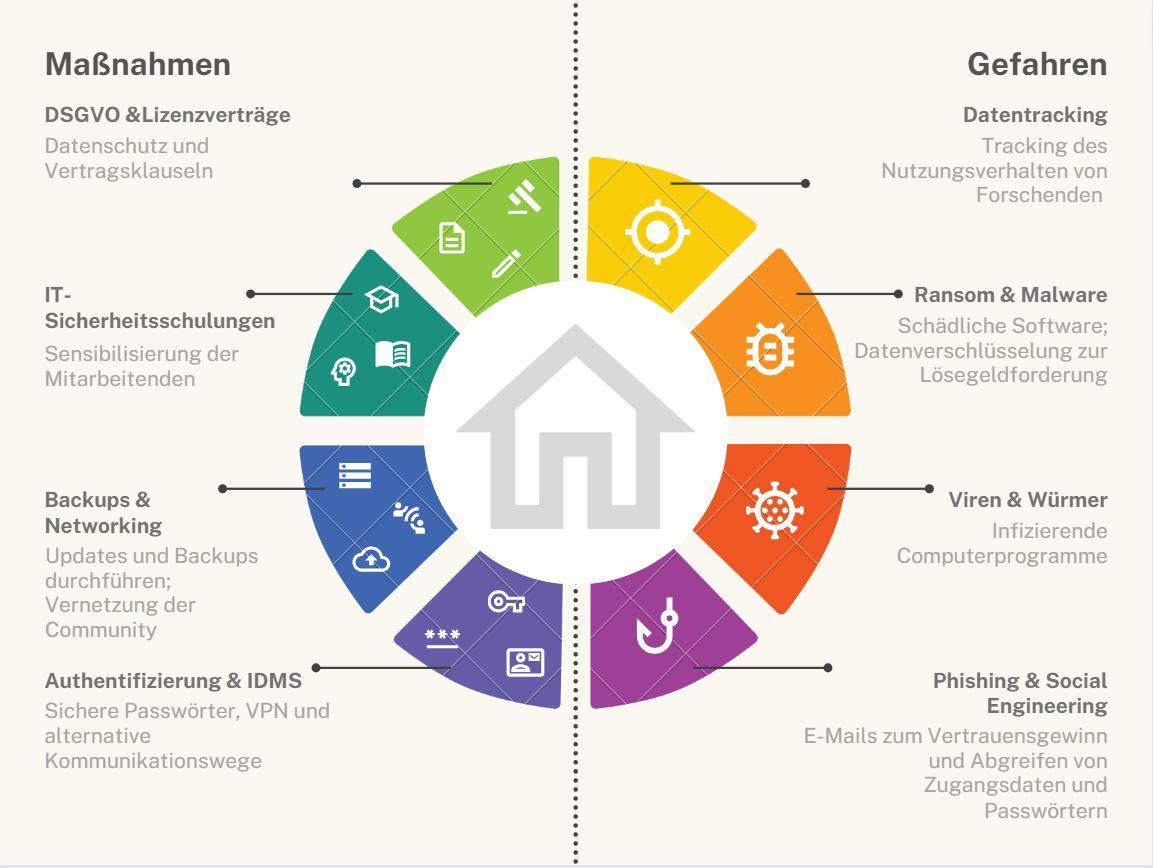
\includegraphics{media/massnahmen-und-praevention.jpg}

}

\caption{\label{fig-massnahmen-praevention}Übersicht über mögliche
Gefahrenquellen und Maßnahmen zur Prävention sowie im Fall eines
Schadens}

\end{figure}%

Zum einen muss intern (mit vorbereiteten Notfallgeräten oder
ggf.~privaten Endgeräten) und extern (mit Dienstleister*innen,
Bibliothekspartner*innen, Bibliotheksnutzer*innen) kommuniziert werden
u.\,a.~über den Vorfall, und ggf. weiterlaufende Dienste (cloudbasierte
und von Drittanbieter*innen). Besonders cloudbasierte Dienste können im
Notfall evt. gute Alternativlösungen bieten. Das gilt auch für
alternative Loginverfahren z.\,B.~bei extern gehosteten Plattformen für
E-Ressourcen, wenn das IDMS nicht zur Verfügung steht.

Ist das BMS einer Bibliothek cloudbasiert, kann ein Ausleihbetrieb mit
Notfallgeräten schneller wieder aufgenommen werden, da die Daten vor dem
Hacker besser geschützt sind. Ähnlich kann man mit eigenen Dokumenten
vorgehen, indem das Active Directory des eigenen Systems ein tägliches
Update erstellt und z.\,B. im CSV-Format an eine Cloud exportiert. Im
einfachsten Fall betrifft es nur Notfalldokumente, die einem Krisenstab
zugänglich sind. Tritt ein Notfall ein, kann man über die
Standard-Benutzeroberfläche der Cloud die gesicherten Skripte starten.
Der Cloudbetreiber sollte Erfahrungen mit Notfalllösungen und
-umgebungen haben. Trotzdem sollte die Bibliothek ihre Datensicherung
gut planen und cloudbasierte oder andere netzwerkunabhängige Backups
länger vorhalten (mindestens 14 Tage), um auf nicht infizierte
Sicherungen zurückgreifen zu können. Es ist auch nicht auszuschließen,
dass die Angreifer die Zugangsdaten für die Datensicherung herausfinden
können. Daher sollte ggf.~eine Verschlüsselung der Datensicherung in
Erwägung gezogen werden. Genauso gilt es, die Wiederherstellung der
Daten zu planen und zu üben. Unerlässlich ist auch eine gute
Dokumentation der gesamten Notfall-Architektur.

Zum anderen sind alternative Abläufe aufzubauen, um wieder an der
digitalen Arbeitswelt teilzunehmen und den Bibliotheksbetrieb
weitestgehend wieder anbieten zu können.

Die kommunikativen Anforderungen sind wie die organisatorischen als sehr
hoch einzuschätzen, da Informationseinrichtungen mit ihren analogen
Begegnungsmöglichkeiten Schnittstellen für eine ganze Hochschule sein
können. Für beide Aufgaben können andere Bibliotheken und externe Firmen
Unterstützung bieten.

Stehen Plan und eine Notfallumgebung, ist es unerlässlich, regelmäßige
Notfallübungen durchzuführen. Damit trainiert man die Abläufe und kann
diese regelmäßig überprüfen und optimieren (Müller 2023). Die dadurch
entstehende Routine kann Sicherheit für den Ernstfall geben. Dennoch
darf man nicht unterschätzen, dass ein Angriff auch persönliche
Auswirkungen auf alle Betroffenen hat.

\section{Fazit}\label{fazit}

Lässt man die Informationen in diesem Kapitel noch einmal Revue
passieren, bleibt als abschließendes Fazit frei nach Ringelnatz nur zu
sagen: „Sicher ist, dass nichts sicher ist. Selbst das nicht``. Trotzdem
ist man der Gefahr nicht hilflos ausgeliefert. Durch Präventivmaßnahmen,
Notfall-Systeme und Pläne kann man einen Angriff wohl nicht verhindern.
Man kann jedoch versuchen, den Schaden und die daraus folgenden
Belastungen so gering wie möglich zu halten. In vielen Bibliotheken
entstehen derzeit individuelle Sicherheitskonzepte und neue
Sicherheitsmaßnahmen. Die nächsten Monate und Jahre werden zeigen, mit
welchen neuen Strategien sich Bibliotheken vor Cyberangriffen schützen
und sich auf diese vorbereiten können.

\bookmarksetup{startatroot}

\chapter{Daten \& Metadaten}\label{sec-metadaten}

\begin{tcolorbox}[enhanced jigsaw, leftrule=.75mm, toprule=.15mm, left=2mm, opacityback=0, arc=.35mm, colback=white, breakable, colframe=quarto-callout-note-color-frame, rightrule=.15mm, bottomrule=.15mm]
\begin{minipage}[t]{5.5mm}
\textcolor{quarto-callout-note-color}{\faInfo}
\end{minipage}%
\begin{minipage}[t]{\textwidth - 5.5mm}

\vspace{-3mm}\textbf{Zusammenfassung}\vspace{3mm}

Die Beschreibung von Ressourcen mit standardisierten Metadaten bildet
eine zentrale Voraussetzung für die meisten an Bibliotheken angebotenen
IT-Dienste. Das vorliegende Kapitel gibt einen Überblick über die
Thematik, indem es
\hyperref[grundlegende-begrifflichkeiten]{grundlegende Begriffe}
einführt, wichtige \hyperref[metadatenstandards]{Metadatenstandards}
vorstellt und
\hyperref[datenverarbeitungsprozess-in-bibliotheken]{Prozesse der
Datenverarbeitung} in Bibliotheken erläutert.

\end{minipage}%
\end{tcolorbox}

\section{Einleitung}\label{einleitung-5}

Für die Sammlung und Bereitstellung von Informationen werden von
Bibliotheken Ressourcen unterschiedlichster Form (Bücher, Filme,
Forschungsdaten \ldots) nachgewiesen. Zur Verwaltung der Ressourcen
werden diese mit \textbf{Metadaten} beschrieben. Neben diesen Metadaten
enthalten bibliothekarische Informationssysteme zunehmend auch die
dazugehörigen \textbf{digitalen Inhalte} wie sogenannte Volltexte,
Digitalisate und Forschungsdaten (Kapitel~\ref{sec-digitalisierung} und
Kapitel~\ref{sec-forschungsnahe-dienste}). Viele der im Folgenden
beschriebenen Grundlagen zu Eigenschaften, Arten und Verarbeitung von
Daten gelten sowohl für Metadaten als auch für digitale Inhalte.

\section{Grundlegende
Begrifflichkeiten}\label{grundlegende-begrifflichkeiten}

\subsection{Daten}\label{daten}

Im Wesentlichen bestehen Daten im Sinne dieses Buchs aus einer Folge von
Bits. Abgesehen von ihrer Anzahl in Bytes lässt sich auf dieser Ebene
allerdings nichts weiter über Daten sagen. Uns interessiert daher mehr,
wofür die Daten stehen~-- beispielsweise für eine Jahreszahl, ein Bild
oder für den Titel eines Dokuments. Dabei besteht ein Unterschied
zwischen

\begin{itemize}
\item
  der Struktur von Daten (\textbf{Syntax})
\item
  und der Bedeutung von Daten (\textbf{Semantik}).
\end{itemize}

Zur Interpretation von Daten dienen \textbf{Kodierungen} in Form von
Datenformaten und \hyperref[identifikatoren]{Identifikatoren}. Wo genau
jeweils die Grenze zwischen Syntax und Semantik liegt, hängt davon ab,
auf welcher Ebene und mit welcher Kodierung Daten betrachtet und
verarbeitet werden (siehe Tabelle~\ref{tbl-daten-ebenen}):

\begin{longtable}[]{@{}lll@{}}
\toprule\noalign{}
Struktur & Bedeutung & Kodierung \\
\midrule\noalign{}
\endfirsthead
\toprule\noalign{}
Struktur & Bedeutung & Kodierung \\
\midrule\noalign{}
\endhead
\bottomrule\noalign{}
\endlastfoot
\texttt{2024-02-24} & Der 24. Februar 2024 & ISO 8601 \\
\texttt{1100001} & Die Zahl 97 (64+32+1) & Byte als Zahl \\
\texttt{97} & Der Buchstabe „a`` & ASCII oder Unicode \\
\texttt{a} & Unterfeld für Haupttitel & Feld \texttt{021A} im PICA+
Format \\
\texttt{a} & Unterfeld für Umfangsangabe & Feld \texttt{300} im MARC21
Format \\
\caption{Beispiele für Syntax und Semantik von Daten auf verschiedenen
Ebenen}\label{tbl-daten-ebenen}\tabularnewline
\end{longtable}

Ein Großteil der
\hyperref[datenverarbeitungsprozess-in-bibliotheken]{Datenverarbeitung}
besteht darin, Daten, zum Beispiel im Rahmen von
\hyperref[etl-prozess]{ETL-Prozessen}, von einer Kodierung in eine
andere Kodierung zu überführen, um sie anschließend leichter
interpretieren zu können. Bei der Konvertierung von Daten von einem in
ein anderes Datenformat reduziert sich das implizite Datenmodell der
Konvertierung auf den kleinsten gemeinsamen Nenner beider Formate.

Zur Beschreibung von Daten dienen

\begin{itemize}
\item
  formale \textbf{Schemata} auf Ebene der Syntax und
\item
  \textbf{Datenmodelle} auf Ebene der Semantik.
\end{itemize}

Leider liegen beide oft nicht explizit vor, sondern müssen anhand von
Beispielen, Anwendungen und Dokumentation mühsam ermittelt werden. Im
Idealfall entsprechen Daten einem klar definierten Datenformat.

\begin{tcolorbox}[enhanced jigsaw, leftrule=.75mm, toprule=.15mm, left=2mm, opacityback=0, arc=.35mm, colback=white, breakable, colframe=quarto-callout-tip-color-frame, rightrule=.15mm, bottomrule=.15mm]
\begin{minipage}[t]{5.5mm}
\textcolor{quarto-callout-tip-color}{\faLightbulb}
\end{minipage}%
\begin{minipage}[t]{\textwidth - 5.5mm}

Mit dem \textbf{Resource Description Framework (RDF)} kodierte Daten
werden auch als „semantisch`` bezeichnet. Die Kodierung erfolgt dabei
nicht mit Feldern oder Tabellen, sondern in Form von so genannten
RDF-Tripeln aus Subjekt, Prädikat und Objekt. Durch Verwendung
gemeinsamer \hyperref[identifikatoren]{Identifikatoren} in mehreren
Tripeln entstehen
\hyperref[datenmodelle-und-ontologien]{Wissensgraphen}, die in
speziellen Datenbanken (\emph{Triplestores}) gespeichert und abgefragt
werden können.

Die Bedeutung von RDF-Daten ergibt sich allerdings, wie bei allen
Kodierungen, erst aus der Dokumentation von Datenelementen und ihrer
Interpretation in praktischen Anwendungen.

\end{minipage}%
\end{tcolorbox}

\subsection{Datenformate}\label{datenformate}

Datenformate definieren eine Struktur, die sich in einer oder in
mehreren austauschbaren Syntaxvarianten ausdrücken lässt und deren
Bedeutung durch ein Datenmodell festgelegt ist. Beispielsweise definiert
der Unicode-Standard eine Menge von Schriftzeichen (Buchstaben,
Sonderzeichen, Emojis \ldots) und verschiedene Verfahren, um
Zeichenketten in Bytes zu kodieren (UTF-8, UTF-16 \ldots).
Syntaxvarianten werden auch als \textbf{Serialisierung} bezeichnet. Die
meisten Datenformate haben nur eine Serialisierung, sodass Format und
Syntax meist synonym verwendet werden. Einzelne Syntaxelemente
entsprechen Bestandteilen im Datenmodell (siehe Tabelle~\ref{tbl-xml}),
daher werden in der Beschreibung von Daten auch diese beiden Ebenen
meist nicht sauber getrennt.

\begin{longtable}[]{@{}ll@{}}
\toprule\noalign{}
XML-Syntax & XML-Modell \\
\midrule\noalign{}
\endfirsthead
\toprule\noalign{}
XML-Syntax & XML-Modell \\
\midrule\noalign{}
\endhead
\bottomrule\noalign{}
\endlastfoot
\texttt{\textless{}name\ /\textgreater{}} oder
\texttt{\textless{}name\textgreater{}...\textless{}/name\textgreater{}}
& XML-Element \\
\texttt{name="Inhalt"} & XML-Attribut \\
\texttt{\textless{}!-\/-\ ...\ -\/-\textgreater{}} & Kommentar \\
\caption{Einige Bestandteile des
XML-Formats}\label{tbl-xml}\tabularnewline
\end{longtable}

Als Faustregel kann gelten, dass bei statischer Betrachtung von Daten
der Bezug auf ihre Syntax sinnvoll ist, während zur Verarbeitung von
Daten eher auf die Bestandteile ihrer Modelle Bezug genommen werden
sollte.

Datenformate lassen sich grob in zwei Kategorien unterteilen:

\begin{itemize}
\item
  \textbf{Strukturierungssprachen} wie CSV, XML, JSON und RDF
  ermöglichen es, Daten in kleinere Einheiten zu unterteilen und
  miteinander in Beziehung zu setzen. Die Sprachen basieren auf
  allgemeinen Ordnungsprinzipien (Felder, Tabellen, Hierarchien,
  Netzwerke \ldots) und ihre Modelle haben darüber hinaus keine eigene
  Semantik. Die einfachste Strukturierungssprache ist das Prinzip der
  Zeichenkette.
\item
  \textbf{Anwendungsformate} legen die Struktur von Daten für konkrete
  Arten von Inhalten fest (\hyperref[metadatenformate]{Metadatenformate}
  zur Beschreibung von Dokumenten, Bildformate für Bilder \ldots). Ihre
  Modelle verweisen letztendlich auf reale Objekte und Eigenschaften.
  Viele Anwendungsformate sind ihrerseits mittels einer
  Strukturierungssprache kodiert, zum Beispiel basiert das
  DataCite-Format zur Beschreibung von Forschungsdaten auf dem
  XML-Modell.
\end{itemize}

Darüber hinaus gibt es besondere Formate, deren Anwendung in der
Verarbeitung von Daten liegt. Neben Programmiersprachen, die selbst
nicht als Datenformate betrachtet werden, sind dies folgende Sprachen:

\begin{itemize}
\item
  \textbf{Schemasprachen} wie XML Schema, JSON Schema und nicht zuletzt
  \emph{reguläre Ausdrücke} dienen der formalen Beschreibung der Syntax
  von Datenformaten. Dabei bezieht sich jede Schemasprache auf eine
  Strukturierungssprache (\emph{XML Schema} für XML-Formate,
  \emph{Avram} für feldbasierte Formate \ldots).
\item
  \textbf{Abfragesprachen} dienen dem Verweis auf einzelne Teile von
  Datensätzen. Sie beziehen sich ebenfalls immer auf eine
  Strukturierungssprache (zum Beispiel XPath für XML, JSON Path für JSON
  \ldots) und sind für die Verarbeitung von Daten notwendig.
\item
  \textbf{Modellierungssprachen} helfen bei der Beschreibung von
  Datenmodellen. Die häufigsten Modellierungssprachen basieren auf dem
  Entity-Relationship-Modell. Da zwischen Syntax und Semantik irgendwann
  die reine Datenebene verlassen werden muss, sind die wichtigsten
  Mittel zur Datenmodellierung allerdings Diagramme und Beschreibungen
  in natürlicher Sprache.
\end{itemize}

\begin{tcolorbox}[enhanced jigsaw, leftrule=.75mm, toprule=.15mm, left=2mm, opacityback=0, arc=.35mm, colback=white, breakable, colframe=quarto-callout-tip-color-frame, rightrule=.15mm, bottomrule=.15mm]
\begin{minipage}[t]{5.5mm}
\textcolor{quarto-callout-tip-color}{\faLightbulb}
\end{minipage}%
\begin{minipage}[t]{\textwidth - 5.5mm}

Das \textbf{Entity-Relationshop-Modell} ist eine Modellierungssprache
die meist für relationale Datenbanken verwendet wird, aber auch
unabhängig davon verwendet werden kann. Dabei werden in einem
ER-Diagramm Objekttypen (Entitäten) und ihre Beziehungsarten dargestellt
(siehe Beispiel Abbildung~\ref{fig-er-diagram}). Eine graphische Syntax
für erweiterte ER-Diagramme ist die Unified Modeling Language
(\emph{UML}).

\begin{figure}[H]

\centering{


\includegraphics{index_files/mediabag/media/er-modell.pdf}

}

\caption{\label{fig-er-diagram}ER-Diagramm zur Beschreibung eines
Datenmodells von Sitzbänken}

\end{figure}%

\end{minipage}%
\end{tcolorbox}

Die Verwendung von Schema-, Abfrage- und Modellierungssprachen hilft,
häufig auftretende Fehler bei der (Meta-)Datenverarbeitung zu vermeiden.
Ein Beispiel hierfür ist das \emph{Resource Description Framework}
(\emph{RDF}) mit dazugehörigen Schemasprachen
(\emph{SHACL}/\emph{ShEx}), Abfragesprachen (\emph{SPARQL}) und
Modellierungssprachen (\emph{RDFS}/\emph{OWL}). In anderen Fällen wird
aus Mangel an Werkzeugen und Kenntnissen auf spezielle Datensprachen
verzichtet und stattdessen auf allgemeine Programmiersprachen
zurückgegriffen.

Eine ausführlichere Beschreibung von Datenformaten mit
bibliothekarischem Schwerpunkt bietet die Datenbank
\href{https://format.gbv.de/}{format.gbv.de}. Grundlagen von Metadaten
und Ontologien vermitteln Assfalg (2023) und Rölke und Weichselbraun
(2023).

In der Praxis werden Daten in einem Datenformat zusätzlich durch
anwendungsspezifische Auslegungen und Einschränkungen geprägt, darunter
Formatvarianten, Metadatenprofile bzw.~Anwendungsprofile,
Erfassungsregeln und die jeweilige Erfassungspraxis.

\begin{tcolorbox}[enhanced jigsaw, leftrule=.75mm, toprule=.15mm, left=2mm, opacityback=0, arc=.35mm, colback=white, breakable, colframe=quarto-callout-tip-color-frame, rightrule=.15mm, bottomrule=.15mm]
\begin{minipage}[t]{5.5mm}
\textcolor{quarto-callout-tip-color}{\faLightbulb}
\end{minipage}%
\begin{minipage}[t]{\textwidth - 5.5mm}

\textbf{Reguläre Ausdrücke} sind das gängigste Mittel zur Beschreibung
der Syntax von Daten. Gleichzeitig können mit ihnen Zeichenketten nach
Mustern durchsucht werden. Ein regulärer Ausdruck für die Syntax einer
ISBN-13 mit optionalen Trennstrichen ist beispielsweise:

\begin{verbatim}
(97[89])-?([0-9]{1,5})-?([0-9]+)-?([0-9]+)-?[0-9]
\end{verbatim}

Üblicherweise decken Schemasprachen nicht alle Aspekte eines
Datenformats ab. So lässt sich die Korrektheit der abschließenden
Prüfziffer (\texttt{{[}0-9{]}}) nicht mit einem regulären Ausdruck
überprüfen.

\end{minipage}%
\end{tcolorbox}

\subsection{Identifikatoren}\label{identifikatoren}

Ein wesentlicher Teil von Daten besteht aus Identifikatoren (IDs).
Identifikatoren sind Namen, Nummern oder Codes, die eine eindeutige
Referenzierung gleicher Dinge in unterschiedlichen Kontexten
ermöglichen. Daten aus unterschiedlichen Quellen können miteinander
abgeglichen und kombiniert werden, wenn sie die gleichen Identifikatoren
verwenden.

Neben eher intern genutzten Datensatz-Identifikatoren (z.\,B.~die {PPN}
des Bibliothekssystems PICA oder die ZDB-ID der Zeitschriftendatenbank)
sind vor allem international standardisierte Identifikatoren von
Bedeutung. Beispiele für solche Identifiersysteme mit Relevanz für
bibliothekarische Daten sind die nachfolgenden:

\begin{itemize}
\item
  Die \emph{International Standard Book Number} (\textbf{ISBN}) wird von
  Verlagen für Bücher vergeben. Seit 2007 ist die 13-stellige ISBN Teil
  des EAN-Barcode-Systems.
\item
  Die \emph{International Standard Serial Number} (\textbf{ISSN})
  identifiziert Zeitschriften und Schriftenreihen.
\item
  Der \emph{Digital Object Identifier} (\textbf{DOI}) identifiziert
  digitale Publikationen in elektronischen Zeitschriften und
  Repositorien.
\item
  Der \emph{International Standard Identifier for Libraries and Related
  Organisations} (\textbf{ISIL}) referenziert Bibliotheken, Archive,
  Museen und verwandte Einrichtungen.
\item
  Die \emph{Open Researcher and Contributor ID} (\textbf{ORCID})
  identifiziert Autor*innen von wissenschaftlichen Publikationen.
\item
  Der \emph{Uniform Resource Locator} (\textbf{URL}) dient als Adresse
  einer digitalen Ressource im Web und wird teilweise gleichzeitig als
  deren Identifikator eingesetzt.
\item
  Das System der \emph{Uniform Resource Identifier} (\textbf{URI})
  ermöglicht die Vereinigung verschiedener Identifier-Systeme und bildet
  die Grundlage von \emph{RDF} und Linked Open Data (\emph{LOD}).
\end{itemize}

Gemeinsam ist den Identifikatoren, dass sie jeweils eine definierte
Syntax haben (z.\,B.~\texttt{XXXX-XXXY} im Falle der ISSN, wobei
\texttt{X} für eine Ziffer und \texttt{Y} für eine Prüfziffer steht),
deren Bestandteile hierarchisch von einer zentralen Instanz festgelegt
werden. Nach dem Prinzip des Namensraums kann dabei die Vergabe von
Teilen an untergeordnete Organisationen delegiert werden. Beispielsweise
werden ISIL für Bibliotheken in Deutschland beginnend mit dem Präfix
„DE-`` durch die
\href{https://sigel.staatsbibliothek-berlin.de/}{ISIL-Agentur an der
Staatsbibliothek zu Berlin} verwaltet.

Im Gegensatz dazu gibt es zur Identifizierung von digitalen Objekten
auch dezentrale Identifikatoren in Form von Prüfsummen, die sich
automatisch aus den vorhandenen Daten berechnen lassen (SHA-Summe,
IPFS-Adresse, Prüfziffer \ldots).

\subsection{Normdaten}\label{normdaten}

Einfache kontrollierte Vokabulare bestehen aus normierten Listen von
eindeutigen Benennungen~-- beispielsweise könnte in einem
Gemüse-Vokabular festgelegt sein, dass immer „Karotte`` statt „Möhre``
verwendet werden muss. Wird jeder Eintrag mit einem künstlichen
\hyperref[identifikatoren]{Identifikator} versehen, muss die Benennung
selbst nicht eindeutig sein. Existiert eine Datenbank zum Nachschlagen
dieser IDs, so wird diese auch als \emph{Normdatei} bezeichnet. Ihre
Datensätze dienen als \emph{Normdaten} der eindeutigen Identifizierung
von Personen, Organisationen, geographischen oder administrativen
Einheiten, Themen oder anderen Entitäten an verschiedenen Stellen. Ein
Normdatensatz besteht mindestens aus einem Identifikator und einer
Vorzugsbenennung als primärer Name. Oft gibt es weitere identifizierende
Merkmale wie alternative Benennungen, Lebensdaten von Personen,
Ortsangaben u.\,Ä.~sowie Verknüpfungen zwischen verschiedenen Entitäten.

\begin{tcolorbox}[enhanced jigsaw, leftrule=.75mm, toprule=.15mm, left=2mm, opacityback=0, arc=.35mm, colback=white, breakable, colframe=quarto-callout-tip-color-frame, rightrule=.15mm, bottomrule=.15mm]
\begin{minipage}[t]{5.5mm}
\textcolor{quarto-callout-tip-color}{\faLightbulb}
\end{minipage}%
\begin{minipage}[t]{\textwidth - 5.5mm}

Umfang und Komplexität von Normdateien reichen von einfachen Listen bis
zu komplexen \hyperref[datenmodelle-und-ontologien]{Ontologien und
Wissensgraphen}. Ein prominentes bibliothekarisches Beispiel einer
Normdatei ist die Gemeinsame Normdatei ({GND}), in der neben Personen
auch Körperschaften, Veranstaltungen, Geografika, Werke und
Sachschlagwörter miteinander vernetzt sind.

\end{minipage}%
\end{tcolorbox}

Zur Anreicherung von Daten mit Normdaten mittels \emph{Entity
Recognition} (Erkennung von Entitäten in Daten) und \emph{Entity
Linking} (Abgleich von Entitäten mit IDs anderer Normdateien) sollte
unterschieden werden zwischen:

\begin{itemize}
\item
  Normdateien mit Entitäten wie Personen (ORCID), Publikationen (DOI,
  ISBN), Sprachen (ISO 639) etc., die sich grundsätzlich eindeutig
  unterscheiden lassen sowie
\item
  Normdateien, deren abstrakte Entitäten von Kontext und Modellierung
  abhängen (Klassifikationen, Thesauri \ldots).
\end{itemize}

Zur Verwaltung von Normdaten gibt es einige Datenformate wie \emph{MARC
21 for Authority Data} und \emph{ISAAR (CPF)}. Als gemeinsamer Nenner
auch außerhalb des Bibliotheksbereichs gilt das RDF-basierte
\emph{Simple Knowledge Organization System} (\emph{SKOS}), für das mit
JSKOS auch eine JSON-Variante existiert. Vor allem kleinere oder
speziellere Normdateien (z.\,B.~Codelisten im Rahmen der
Katalogisierung) liegen allerdings selten in maschinenlesbarer Form vor.

Das \href{https://bartoc.org/}{\emph{Basic Register of Thesauri,
Ontologies \& Classifications}} (BARTOC) erfasst Informationen zu
Normdateien aller Art, darunter auch Verfahren zum technischen Zugriff.

\section{Metadatenstandards}\label{metadatenstandards}

Neben allgemeinen \hyperref[datenformate]{Datenformaten} sind für die
Bibliotheks-IT vor allem Metadatenformate zur Beschreibung von
Dokumenten relevant. Die meisten der im Folgenden beschriebenen
Metadatenformate spielen außerhalb von Kultureinrichtungen keine
wesentliche Rolle. Für digitale Objekte (\emph{METS/MODS}, \emph{LIDO},
\emph{CDWA}, \emph{EN 15907}, \emph{EAD} \ldots, siehe
Kapitel~\ref{sec-digitalisierung}) und für Forschungsdaten (DataCite,
siehe Kapitel~\ref{sec-forschungsnahe-dienste}) gibt es darüber hinaus
spezielle Formate.

\subsection{Arten von Metadaten}\label{sec-arten-von-metadaten}

Folgende Arten von Metadaten können nach ihrer Funktion unterschieden
werden:

\begin{itemize}
\item
  \textbf{Deskriptive} (= beschreibende) \textbf{Metadaten} zur
  Identifizierung und inhaltlichen Beschreibung wie Titel, Verfasser*in,
  Schlagwörter etc.
\item
  \textbf{Administrative} (= Verwaltungs-)\textbf{Metadaten} wie Angaben
  zu Herkunft, Speicherung, Zugriffsrechten, Verwaltung etc.
\item
  \textbf{Strukturelle Metadaten} über den Aufbau von Dokumenten wie die
  Einteilung in einzelne Kapitel, Abschnitte, eingebundene Medien etc.
  Die Grenze zwischen digitalen Inhalten und ihrer Struktur ist
  allerdings mitunter fließend.
\item
  \textbf{Technische Metadaten} zu Merkmalen wie Umfang, verwendeten
  Datenformaten etc.
\end{itemize}

Je nach Anwendung gibt es spezielle Metadatenformate oder es werden
verschiedene Arten von Beschreibungen in einem Format zusammengefasst.

\subsection{Feldbasierte bibliothekarische
Metadatenformate}\label{feldbasierte-bibliothekarische-metadatenformate}

\textbf{Machine-Readable Cataloging (MARC)} ist das älteste und noch
immer wichtigste Format für den Austausch von Daten zwischen
Bibliotheken. Die aktuell relevante Variante ist MARC 21, insbesondere
das Format MARC 21 für bibliografische Daten. Neben der binären
Kodierung kann MARC 21 auch in XML (siehe Abbildung~\ref{fig-marcxml})
und JSON kodiert werden. Viele Eigenheiten und Probleme des Formats sind
historisch bedingt, die Alternative BIBFAME konnte sich noch nicht
durchsetzen.

\textbf{PICA} ist das von MARC inspirierte Datenformat der
Katalogisierungssysteme {CBS} und \emph{LBS} (Voß 2022). Das wichtigste
Anwendungsprofil ist das K10plus-Internformat.

\textbf{MAB} und \textbf{allegro} sind ebenfalls an MARC angelehnte,
feldbasierte Formate aus dem deutschsprachigen Raum, die allerdings nur
noch sporadisch verwendet werden.

\begin{figure}

\centering{

\scriptsize

\begin{Shaded}
\begin{Highlighting}[]
\FunctionTok{\textless{}?xml}\OtherTok{ version=}\StringTok{"1.0"}\OtherTok{ encoding=}\StringTok{"UTF{-}8"}\FunctionTok{?\textgreater{}}
\NormalTok{\textless{}}\KeywordTok{record}\OtherTok{ xmlns=}\StringTok{"http://www.loc.gov/MARC21/slim"}\NormalTok{\textgreater{}}
\NormalTok{  \textless{}}\KeywordTok{leader}\NormalTok{\textgreater{} cam a22 4500\textless{}/}\KeywordTok{leader}\NormalTok{\textgreater{}}
\NormalTok{  \textless{}}\KeywordTok{datafield}\OtherTok{ tag=}\StringTok{"245"}\OtherTok{ ind1=}\StringTok{"1"}\OtherTok{ ind2=}\StringTok{"0"}\NormalTok{\textgreater{}}
\NormalTok{    \textless{}}\KeywordTok{subfield}\OtherTok{ code=}\StringTok{"a"}\NormalTok{\textgreater{}Handbuch IT in Bibliotheken\textless{}/}\KeywordTok{subfield}\NormalTok{\textgreater{}}
\NormalTok{  \textless{}/}\KeywordTok{datafield}\NormalTok{\textgreater{}}
\NormalTok{  \textless{}}\KeywordTok{datafield}\OtherTok{ tag=}\StringTok{"540"}\OtherTok{ ind1=}\StringTok{" "}\OtherTok{ ind2=}\StringTok{" "}\NormalTok{\textgreater{}}
\NormalTok{    \textless{}}\KeywordTok{subfield}\OtherTok{ code=}\StringTok{"a"}\NormalTok{\textgreater{}Namensnennung 3.0 Deutschland\textless{}/}\KeywordTok{subfield}\NormalTok{\textgreater{}}
\NormalTok{    \textless{}}\KeywordTok{subfield}\OtherTok{ code=}\StringTok{"f"}\NormalTok{\textgreater{}CC{-}BY 3.0 DE\textless{}/}\KeywordTok{subfield}\NormalTok{\textgreater{}}
\NormalTok{    \textless{}}\KeywordTok{subfield}\OtherTok{ code=}\StringTok{"u"}\NormalTok{\textgreater{}https://creativecommons.org/licenses/by/3.0/de/\textless{}/}\KeywordTok{subfield}\NormalTok{\textgreater{}}
\NormalTok{  \textless{}/}\KeywordTok{datafield}\NormalTok{\textgreater{}}
\NormalTok{  \textless{}}\KeywordTok{datafield}\OtherTok{ tag=}\StringTok{"856"}\OtherTok{ ind1=}\StringTok{"4"}\OtherTok{ ind2=}\StringTok{"0"}\NormalTok{\textgreater{}}
\NormalTok{    \textless{}}\KeywordTok{subfield}\OtherTok{ code=}\StringTok{"u"}\NormalTok{\textgreater{}https://it{-}in{-}bibliotheken.de/\textless{}/}\KeywordTok{subfield}\NormalTok{\textgreater{}}
\NormalTok{    \textless{}}\KeywordTok{subfield}\OtherTok{ code=}\StringTok{"z"}\NormalTok{\textgreater{}kostenfrei\textless{}/}\KeywordTok{subfield}\NormalTok{\textgreater{}}
\NormalTok{  \textless{}/}\KeywordTok{datafield}\NormalTok{\textgreater{}}
\NormalTok{\textless{}/}\KeywordTok{record}\NormalTok{\textgreater{}}
\end{Highlighting}
\end{Shaded}

\normalsize

}

\caption{\label{fig-marcxml}Ein gekürzter Beispieldatensatz in MARC-XML}

\end{figure}%

\subsection{XML-basierte Datenformate}\label{xml-basierte-datenformate}

\textbf{METS} und \textbf{MODS} sind zwei zusammen im Bereich
Digitalisierung (Kapitel~\ref{sec-digitalisierung}) eingesetzte Formate
für strukturelle und administrative (METS) sowie bibliografische
Metadaten (MODS). Strukturdaten in METS ermöglichen granulare Gliederung
und Verlinkung von Objekten, wobei mögliche Typen und Beziehungen in
Regelsätzen definiert sind.

\emph{\href{https://wiki.deutsche-digitale-bibliothek.de/pages/viewpage.action?pageId=19010182}{Encoded
Archival Description}} (\textbf{EAD}) ist der zentrale dokumentarische
XML-Standard zur Beschreibung von archivischen Findmitteln.

\textbf{LIDO} ist ein etabliertes Austauschformat für den
Museumsbereich.

\textbf{DataCite} ist ein bibliografisches Datenformat, insbesondere zur
Beschreibung von Forschungsdaten
(Kapitel~\ref{sec-forschungsnahe-dienste}).

\subsection{Datenmodelle und
Ontologien}\label{datenmodelle-und-ontologien}

\textbf{Dublin Core} bzw.~das Dublin Core Metadata Element Set
(\textbf{DCMES}) hat als kleinster gemeinsamer Nenner der meisten
Metadatenstandards die größte Verbreitung. Es besteht aus 15
Basiselementen wie „creator``, „title``, „date`` und „description`` und
Erweiterungen mit den DCMI Metadata Terms wie „Alternative Title``,
„Date Created`` und „Date Available``.

Die \emph{Functional Requirements for Bibliographic Records}
(\textbf{FRBR}) sind ein sehr abstraktes Metadatenmodell. Sie beinhalten
insbesondere eine Einteilung von bibliografischen Entitäten in die
Beschreibungsebenen „work``, „expression``, „manifestation`` und
„item``.

Die \textbf{BIBFRAME}-Ontologie wurde entwickelt, um MARC auf Grundlage
von RDF zu ersetzen. Die wesentlichen Elemente sind „work``, „instance``
und „item`` sowie damit verbundene Eigenschaften und Entitätstypen.

\textbf{Schema.org} ist eine allgemeine Ontologie für strukturierte
Daten in Webseiten.

\begin{tcolorbox}[enhanced jigsaw, leftrule=.75mm, toprule=.15mm, left=2mm, opacityback=0, arc=.35mm, colback=white, breakable, colframe=quarto-callout-important-color-frame, rightrule=.15mm, bottomrule=.15mm]
\begin{minipage}[t]{5.5mm}
\textcolor{quarto-callout-important-color}{\faExclamation}
\end{minipage}%
\begin{minipage}[t]{\textwidth - 5.5mm}

Eine \textbf{Ontologie} ist ein Datenmodell, das verschiedene Klassen
und Eigenschaften in RDF definiert und so die einheitliche Kodierung und
Verknüpfung verschiedener Datenquellen von Linked Data bis hin zu
umfangreichen Wissensgraphen ermöglicht.

Im Gegensatz zu einfacheren Formen von \hyperref[normdaten]{Normdaten}
geht es bei Ontologien nicht nur um die eindeutige Identifizierung
(Beispiel: ist mit „Bank`` das Gleiche wie „Sitzbank`` oder wie
„Geldinstitut`` gemeint?) sondern auch um Eigenschaften und Beziehungen
(Beispiel: mögliche Größen, Materialien und Orte von Bänken).
\textbf{Wissensgraphen} enthalten neben Ontologien auch konkrete Daten
über Instanzen der Ontologie-Klassen (Beispiel: Liste konkreter
Sitzbänke an einem Ort).

\end{minipage}%
\end{tcolorbox}

\begin{figure}

\centering{

\scriptsize

\begin{Shaded}
\begin{Highlighting}[]
\NormalTok{@prefix bf: \textless{}http://id.loc.gov/ontologies/bibframe/\textgreater{} .}
\NormalTok{@prefix bflc: \textless{}http://id.loc.gov/ontologies/bflc/\textgreater{} .}
\NormalTok{@prefix rdfs: \textless{}http://www.w3.org/2000/01/rdf{-}schema\#\textgreater{} .}
\NormalTok{@prefix xsd: \textless{}http://www.w3.org/2001/XMLSchema\#\textgreater{} .}

\NormalTok{\textless{}http://uri.gbv.de/document/opac{-}de{-}627:ppn:1805728520\textgreater{}}
\NormalTok{  a bf:Electronic, bf:Instance ;}
\NormalTok{  bf:usageAndAccessPolicy [}
\NormalTok{    a bf:UsePolicy ;}
\NormalTok{    rdfs:label}
\NormalTok{      "Namensnennung 3.0 Deutschland",}
\NormalTok{      "https://creativecommons.org/licenses/by/3.0/de/"\^{}\^{}xsd:anyURI ] ;}
\NormalTok{  bf:instanceOf \textless{}http://www.wikidata.org/entity/Q115625546\textgreater{} ;}
\NormalTok{  bf:hasItem [}
\NormalTok{    a bf:Item ;}
\NormalTok{    bf:electronicLocator [}
\NormalTok{      bflc:locator \textless{}https://it{-}in{-}bibliotheken.de/\textgreater{} ;}
\NormalTok{      bf:note [ a bf:Note ; rdfs:label "kostenfrei" ] ] ] .}

\NormalTok{\textless{}http://www.wikidata.org/entity/Q115625546\textgreater{}}
\NormalTok{  a bf:Text, bf:Work ;}
\NormalTok{  bf:title [ a bf:Title ; bf:mainTitle "Handbuch IT in Bibliotheken" ] .}
\end{Highlighting}
\end{Shaded}

\normalsize

}

\caption{\label{fig-bibframe}Der Inhalt des Datensatz
Abbildung~\ref{fig-marcxml} in RDF-Serialisierung Turtle ausgedrückt mit
der BIBFRAME-Ontologie und URIs aus K10plus und Wikidata.}

\end{figure}%

\subsection{Verlagsdaten und
Literaturangaben}\label{verlagsdaten-und-literaturangaben}

Die Formate \emph{ONIX}, \emph{JATS}, \emph{BITS} und \emph{CrossRef
XML} stammen aus dem Verlagsbereich zur Beschreibung von
Zeitschriftenartikeln und Büchern. Sie basieren alle auf XML und sind
für Bibliotheken für den Datenimport relevant. Datenformate für
Literaturangaben (\emph{BibTeX}, \emph{RIS}, \emph{Endnote},
\emph{CSL-JSON} \ldots) werden dagegen zum Export von Katalogdaten
bereitgestellt. Zitationsregeln für Literaturangaben und
Ansetzungsregeln von \emph{ISBD} sind dagegen für den Datenaustausch
eher unbrauchbar. Learning Object Metadata (\emph{LOM}) dient in
verschiedenen lokalen Anpassungen der Beschreibung von Lerneinheiten.

\section{Datenverarbeitungsprozess in
Bibliotheken}\label{datenverarbeitungsprozess-in-bibliotheken}

\subsection{Datenerfassung}\label{datenerfassung}

Traditionell werden bibliothekarische Metadaten durch Katalogisierung
erstellt. Die Verwaltung der Katalogdaten erfolgt entweder lokal oder
gemeinsam in einer \textbf{Verbunddatenbank}. Der Vorteil der
Verbundkatalogisierung liegt darin, dass jedes Dokument nur einmal
zentral beschrieben werden muss, während bei lokaler Katalogisierung
durch \emph{Fremddatenübernahme} nur zum Teil auf vorhandene Kataloge
zurückgegriffen werden kann.

Im Idealfall sollte die Erfassung nach \emph{Autopsie}, also auf
Grundlage des vorliegenden Werkes, durch geschultes Personal und nach
etablierten Regelwerken (\emph{Katalogisierungsrichtlinien}) erfolgen.
Um möglichst viele Publikationen zu erfassen, wird jedoch zunehmend auch
auf anderweitig erfasste Metadaten von Verlagen, Repositorien und aus
anderen Quellen zurückgegriffen. Dazu müssen Daten unterschiedlicher
Erschließungstiefe und -qualität im Rahmen von
\hyperref[etl-prozess]{ETL-Prozessen} gesammelt, analysiert und mit
vorhandenen Daten vereinheitlicht werden. In jedem Fall muss beachtet
werden, dass sich Regeln und Umstände, nach denen Daten erfasst werden,
mit der Zeit ändern können (beispielsweise der Umstieg der
Erfassungsregeln von \emph{RAK} auf {RDA}) und dass das Ergebnis auch
davon abhängt, wie gut überprüft werden kann, was die Anforderungen an
die Daten sind.

Darüber hinaus gibt es Verfahren zur automatischen Erstellung von
Metadaten aus vorhandenen Dokumenten, beispielsweise zur Erkennung und
Auswertung von Literaturangaben und zur thematischen Einordnung von
Dokumenten. Mit diesen Verfahren lassen sich zwar größere Mengen von
Daten erfassen, es muss aber immer mit einer gewissen Fehlerrate
gerechnet werden.

Welche Art und welcher Umfang von Fehlern und Uneinheitlichkeiten bei
der Datenerfassung tolerierbar sind, hängt letztlich davon ab, wozu die
Daten erfasst werden. So gelten beispielsweise für eine historische
Bibliografie andere Maßstäbe als für einen Suchindex.

Nicht zuletzt sollte bedacht werden, dass Geschwindigkeit und Qualität
von Datenerfassung auch von der Usability der Werkzeuge abhängen, mit
denen Daten erstellt, bearbeitet und \emph{analysiert} werden können.

\begin{tcolorbox}[enhanced jigsaw, leftrule=.75mm, toprule=.15mm, left=2mm, opacityback=0, arc=.35mm, colback=white, breakable, colframe=quarto-callout-tip-color-frame, rightrule=.15mm, bottomrule=.15mm]
\begin{minipage}[t]{5.5mm}
\textcolor{quarto-callout-tip-color}{\faLightbulb}
\end{minipage}%
\begin{minipage}[t]{\textwidth - 5.5mm}

Mehr zur bibliothekarischen Datenerfassung in den \emph{Grundlagen der
Informationswissenschaft} (2023), \emph{Teil B}.

\end{minipage}%
\end{tcolorbox}

\subsection{ETL-Prozess}\label{etl-prozess}

Da sich die IT in- und außerhalb von Bibliotheken über verschiedene
Organisationen und Systeme erstreckt, müssen an vielen Stellen Daten von
einer oder mehreren Quellen in ein anderes Informationssystem übertragen
werden. Der grundsätzliche Prozess der Datenintegration, der Quell- und
Zielsysteme verbindet, wird als \textbf{ETL-Prozess} bezeichnet. Der
Prozess aus drei zentralen Schritten „Extract``, „Transform`` und
„Load`` stammt ursprünglich aus dem Bereich des Data Warehousing und
findet sich auch in anderen Anwendungsfällen. Im Folgenden wird er am
Beispiel der Integration von Metadaten in ein Discovery-System
(Kapitel~\ref{sec-discovery}) beschrieben. Abbildung~\ref{fig-etl}
illustriert den generellen ETL-Prozess.

\begin{figure}

\centering{


\includegraphics{index_files/mediabag/media/etl-prozess-kurven.pdf}

}

\caption{\label{fig-etl}Allgemeiner Ablauf eines ETL-Prozesses}

\end{figure}%

\subsubsection{Extraktion}\label{extraktion}

Ziel der \textbf{Extraktion} (Extract) ist die Auswahl und der Abzug
relevanter Daten aus verschiedenen Datenquellen. Hierbei handelt es sich
primär um einen technischen Vorgang, das sogenannte \textbf{Harvesting},
welcher automatisiert oder manuell gestartet werden kann. Der Aufwand
und die Qualität des Harvestings können je nach Datenquelle sehr
unterschiedlich ausfallen. Denkbare Datenquellen sind Dateien,
Datenbanken bzw.~Datenbankabzüge,
\hyperref[schnittstellen]{Schnittstellen} als auch unstrukturierte
Quellen wie z.\,B.~Websites, die mittels Screenscraping erschlossen
werden müssen.

Der Extraktionsvorgang erfolgt bei Bedarf regelmäßig, um die Daten im
Zielsystem aktuell zu halten. Mögliche Aktualisierungsintervalle sind:

\begin{itemize}
\item
  \textbf{periodisch}, das heißt in zeitlich regelmäßigen Abständen
  unabhängig von der jeweiligen Aktualisierung der Daten in den
  Quellsystemen
\item
  \textbf{ereignisgesteuert}, immer wenn bestimmte Bedingungen wie zum
  Beispiel die Änderung von Daten in den Quellsystemen eintreten
\item
  \textbf{manuell}, beispielsweise wenn Daten aus Quellsystemen ad hoc
  importiert werden sollen. Manuelle Aktualisierungen bieten sich vor
  allem an, wenn der Inhalt der Datenquellen weitestgehend statisch ist,
  da die dauerhaft verlässliche Aktualisierung im Zielsystem ohne
  Automatismus nicht garantiert ist.
\end{itemize}

Der Extraktionsvorgang ist technisch relativ einfach handhabbar, wenn
strukturierte \hyperref[datenformate]{Datenformate} und/oder
\hyperref[schnittstellen]{Schnittstellen} existieren~-- die wesentlichen
Aufwände finden sich dann im nachfolgenden Transformationsschritt.
Anders sieht es aus, wenn beispielsweise Daten manuell eingesammelt
werden müssen oder Screenscraping notwendig ist. Beim
\emph{Screenscraping} müssen aufwändig Extraktionsskripte erstellt
werden, um Daten aus Webseiten in ein strukturiertes Format zu
überführen. Diese Skripte sind zudem sehr fehleranfällig und müssen
jedes Mal angepasst werden, wenn die Betreiber*innen der Datenquelle
Veränderungen vornehmen.

Die extrahierten Daten werden in einem Arbeitsbereich abgelegt und dort
im nächsten Prozessschritt aufbereitet.

\subsubsection{Transformation}\label{transformation}

Daten aus verschiedenen Quellsystemen liegen zumeist in
unterschiedlichen Formaten mit unterschiedlichen Datenmodellen vor.
Neben Unterschieden in der Syntax können gleiche Sachverhalte auch auf
semantischer Ebene unterschiedlich beschrieben sein, da die Daten
mitunter für abweichende Anwendungsfälle erfasst wurden. So müssen
beispielsweise in einem Discovery-System (Kapitel~\ref{sec-discovery})
Metadaten zur einfachen Beschreibung so aufbereitet werden, dass sie
auch erweiterte Suchstrategien unterstützen.

Ziel der \textbf{Transformation} ist es, alle Daten in ein einheitliches
Format mit gemeinsamen Datenmodell zu überführen. Dieses Zielformat wird
beim ETL-Prozess auch als \emph{Schema} bezeichnet. Die
Vereinheitlichung des Schemas (\emph{Mapping}) ist ein wesentlicher
Schritt jeder Datenkonvertierung. Zur Minimierung des
Transformationsaufwands dienen gemeinsame Standards wie \emph{MARC21}
als Austauschformat oder die einheitliche Verwendung von RDF-Ontologien.

Über die einfache Konvertierung hinaus sind im Rahmen der Transformation
oft weitere Aufbereitungen zur Vereinheitlichung und Verbesserung der
Datenqualität notwendig. Beispiele hierfür sind:

\begin{itemize}
\item
  Prüfung und \textbf{Vereinheitlichung} der Zeichencodierung auf
  normalisierten Unicode
\item
  formale \textbf{Anpassungen} von Daten wie die Vereinheitlichung von
  Datumsformaten, Ländercodierungen etc.
\item
  Erkennung und Eliminierung von \textbf{Duplikaten}
\item
  Abgleich, Vereinheitlichung und \textbf{Konsistenzprüfung} von
  Aussagen über dieselben Objekte aus verschiedenen Datenquellen
\item
  \textbf{Anreicherung} oder Korrektur von Datensätzen mittels
  Zusatzinformationen aus Normdaten oder anderer zusätzlicher
  Datenquellen
\end{itemize}

Der Aufwand der Transformation sollte nicht unterschätzt werden, da die
Datenqualität verschiedener Datenquellen stark variieren kann und
Qualitätsprobleme oft erst spät entdeckt werden. Zudem können sich
Datenquellen und ihre Qualität zwischen Aktualisierungen ändern. Sofern
die Datenübernahme nicht nur einmalig stattfinden soll
(\emph{Konversion}), ist die Betreuung des Transformationsschrittes eine
Daueraufgabe.

Im Transformationsschritt müssen regelmäßig Massendaten analysiert und
modifiziert werden, daher ist der Einsatz von IT-gestützten
\hyperref[werkzeuge]{Werkzeugen} und Verfahren der
\hyperref[datenanalyse]{Datenanalyse} unerlässlich. Die aus der Analyse
gewonnenen Erkenntnisse müssen wiederum kontinuierlich in die Anpassung
des Schema-Mappings einfließen, damit der Transformationsprozess nicht
ins Stocken gerät.

\subsubsection{Laden}\label{laden}

Auf die Transformation folgt beim \textbf{Laden} (Load) die Überführung
der vereinheitlichten Daten in das Zielsystem~-- beispielsweise in den
Suchindex eines Discovery-Systems (Kapitel~\ref{sec-discovery}). Dabei
dürfen nur Datensätze in Produktivsysteme übernommen werden, die den
Transformationsschritt erfolgreich durchlaufen haben, während für Test-
und Entwicklungssysteme andere Regeln möglich sind.

Das Laden selbst ist ein technisch beherrschbarer Schritt, welcher
optimalerweise darauf abzielt, das Zielsystem ohne Ausfallzeiten aktuell
zu halten. Bei Änderungen des Schemas muss deshalb besonders darauf
geachtet werden, gleichzeitig entsprechende Anpassungen im Zielsystem
vorzunehmen. Daneben ist es bei absehbaren Änderungen ratsam, das Schema
und die Verarbeitung von Daten im Zielsystem von vornherein flexibel zu
gestalten.

\subsubsection{Umsetzung des
ETL-Prozesses}\label{umsetzung-des-etl-prozesses}

Die Umsetzung von Datenkonvertierung und ETL-Prozessen erfolgt im
bibliothekarischen Umfeld oft über selbst entwickelte Skripte für das
Harvesting und die Transformation. Das entsprechende Know-How ist in der
Regel auf wenige Köpfe verteilt und kann auch nicht leicht durch das
Hinzuziehen externer Expertise verfügbar gemacht werden.

Es gibt einige kommerzielle ETL-Komplettlösungen mit Data-Warehouse-
oder Business-Intelligence-Hintergrund. Angesichts der teils erheblichen
Einstiegskosten und zur Vermeidung von \hyperref[vendor-lock-in]{Vendor
Lock-in} sind für Bibliotheken möglichst einfache und allgemeine
\hyperref[werkzeuge]{Werkzeuge zur Datenverarbeitung} meist die bessere
Wahl. Die Vorteile etablierter ETL-Werkzeuge liegen in
Schulungsmöglichkeiten und der Verfügbarkeit externer Expertise. Mit
\emph{Catmandu}, \emph{Metafacture} und \emph{OpenRefine} gibt es
mehrere Open-Source-ETL-Frameworks, deren eingeschränkter
Funktionsumfang und verbesserungswürdige Usability durch Anpassungen für
bibliothekarische Datenformate und Schnittstellen möglicherweise
aufgewogen werden.

Grundsätzlich lassen sich die kontinuierlich anfallenden Aufwände der
Transformation und Qualitätssicherung durch ein ETL-Werkzeug nicht
vermeiden, sondern nur besser handhabbar machen. Dazu sollten die
einzelnen Arbeitsschritte zentral verwaltet und dokumentiert werden,
beispielsweise durch ein Versionskontrollsystem. Durch den Fokus auf
Usability kann mittels ETL-Werkzeugen bibliothekarisches Personal
stärker eingebunden werden. Da hier insbesondere im Bereich der
Programmierung die Einstiegshürden niedriger sind, ist es Fachpersonal
leichter möglich, direkt Änderungen und Optimierungen am ETL-Prozess
vorzunehmen. Bei einer reinen Verankerung von ETL im IT-Bereich sind
solche Eingriffe dagegen nur in Zusammenarbeit von IT und
Metadaten-Expert*innen umsetzbar.

In jedem Fall gehen mit der Einführung von ETL-Werkzeugen in die
bibliothekarische Arbeit immer auch individuelle Anpassungen im Prozess
von Extraktion, Transformation und Laden einher. Dieser Aufwand kann
sowohl gegen die Einführung solcher Werkzeuge sprechen als auch dafür,
vorhandene „Bastellösungen`` zu evaluieren und zu konsolidieren.

\subsection{Werkzeuge}\label{werkzeuge}

Für die Verarbeitung von Daten im Rahmen bibliothekarischer IT-Systeme
werden grundsätzlich die gleichen Werkzeuge verwendet wie außerhalb des
Bibliothekswesens, daher wird an dieser Stelle auf eine allgemeine
Einführung in die Datenverarbeitung verzichtet. Ganz allgemein sind hier
als Werkzeuge

\begin{itemize}
\item
  Mittel zur \textbf{Dateiverwaltung} und ein \textbf{Texteditor}
  unabdingbar,
\item
  allgemeine \textbf{Kommandozeilenprogramme} (\texttt{curl},
  \texttt{sort}, \texttt{grep} \ldots) sehr zu empfehlen und
\item
  \textbf{Programmiersprachen} vor allem für komplexere Aufgaben
  hilfreich.
\end{itemize}

Material und Kurse für die praktischen Grundkenntnisse mit
Bibliotheksbezug finden sich insbesondere in den Bereichen \emph{Data
Librarianship} und \emph{Data Science}.

Werkzeuge für konkrete Datenformate orientieren sich an den zugrunde
liegenden \hyperref[daten]{Strukturierungssprachen}. So gibt es
beispielsweise eigene Editoren oder Editor-Plugins für XML- und
JSON-Daten und entsprechende Kommandozeilentools wie XMLStarlet für XML
und jq für JSON. Für tabellarische Daten eignet sich etwa eine
Tabellenkalkulation oder das tabellenbasierte Werkzeug \emph{OpenRefine}
(\href{https://openrefine.org/}{openrefine.org}).

Für bibliothekarische Datenformate und Schnittstellen gibt es darüber
hinaus einige speziellere Werkzeuge:

\begin{itemize}
\item
  Programmierbibliotheken wie \emph{MARC4J} und \emph{YAZ} erleichtern
  die Datenverarbeitung im Rahmen eigener Programme.
\item
  Anwendungsprogramme wie \emph{WinIBW} und \emph{BibControl} erfordern
  zwar weniger IT-Kenntnisse, sind dafür aber nur eingeschränkt und/oder
  nur für sehr spezielle Aufgaben verfügbar.
\item
  Freie Werkzeuge zum Metadatenmanagement wie die Frameworks
  \emph{Catmandu}
  (\href{http://librecat.org/Catmandu/}{librecat.org/Catmandu}) und
  \emph{Metafacture} (\href{https://metafacture.org/}{metafacture.org}).
\end{itemize}

Für einzelne Anwendungen und Formate gibt es einige weitere Werkzeuge
und es kann sich lohnen, solche Werkzeuge selbst zu entwickeln und als
Open Source zur Verfügung zu stellen. Für das PICA-Format sind derartige
Programme in der \emph{Einführung in die Verarbeitung von PICA-Daten}
(Voß 2022) aufgeführt.

\subsection{Schnittstellen}\label{schnittstellen}

Eine API (Application Programming Interface, auch
Programmierschnittstelle) ist eine definierte Methode zur Abfrage
und/oder Änderung von Daten in einem Informationssystem. Wie die Daten
innerhalb des Systems verwaltet werden, ist dabei nebensächlich. Dieses
Prinzip ermöglicht die Kombination unterschiedlicher
Softwarekomponenten. Wenn möglich, sollten produktunabhängige, offen
dokumentierte APIs verwendet werden. Im Bibliotheksbereich sind
insbesondere folgende APIs relevant:

\begin{itemize}
\item
  \textbf{Z39.50} wurde vor Erfindung des Web zur Suche in
  Bibliotheksdatenbanken entwickelt. Nachfolger ist das XML-basierte
  \emph{Search/Retrieve via URL} (\textbf{SRU}) mit der zugehörigen
  Abfragesprache \emph{Contextual Query Language} (\textbf{CQL}).
\item
  Das \emph{\href{https://www.openarchives.org/pmh/}{Open Archives
  Initiative Protocol for Metadata Harvesting}} (\textbf{OAI-PMH}) dient
  dem Abruf von Metadaten aus Repositorien. Die Daten können nach Datum
  und Teilmengen gefiltert und so in Suchmaschinen und Portalen wie
  \href{https://www.base-search.net/}{BASE} und der
  \href{https://www.deutsche-digitale-bibliothek.de/}{Deutschen
  Digitalen Bibliothek} (DDB) zusammengeführt werden.
\item
  Das \emph{NISO Circulation Interchange Protocol} (\textbf{NCIP}), das
  \emph{Simple Library Network Protocol} (\textbf{SLNP}) und das
  \emph{Standard Interchange Protocol} (\textbf{SIP2}) sind interne APIs
  für Ausleihe und Fernleihe. Sie werden zwischen Bibliotheken,
  Fernleihservern und zur Anbindung von Verbuchungsautomaten eingesetzt
  (Michaelis 2014).
\item
  Die \emph{\href{https://gbv.github.io/paia/}{Patrons Account
  Information API}} (\textbf{PAIA}) ist eine offene Schnittstelle zum
  Zugriff auf Ausleihkonten.
\item
  Die \emph{\href{https://gbv.github.io/daia/}{Document Availability
  Information API}} (\textbf{DAIA}) ist eine offene Schnittstelle zur
  Abfrage der Verfügbarkeit von Medien.
\item
  Mit \textbf{unAPI} können einzelne Datensätze in verschiedenen
  Formaten abgerufen werden.
\item
  Die
  \textbf{\href{https://reconciliation-api.github.io/specs/draft/}{Reconciliation
  Service API}} ermöglicht den Abgleich mit Normdaten zur eindeutigen
  Referenzierung (siehe Abschnitte zu
  \hyperref[identifikatoren]{Identifikatoren} und zu
  \hyperref[normdaten]{Normdaten}).
\item
  Die APIs des \emph{\href{https://iiif.io/}{International Image
  Interoperability Framework}} (\textbf{IIIF}) ermöglicht die
  Referenzierung und Nutzung digitalisierter Werke in externen
  Werkzeugen durch gezielte Verlinkung auf einzelne Bestandteile.
\item
  Über \textbf{SPARQL}-Schnittstellen können RDF-Daten aus
  Wissensgraphen wie zum Beispiel Wikidata abgerufen werden.
\item
  Schnittstellen zur Authentifizierung und Autorisierung wie {LDAP},
  \emph{Shibboleth} und \emph{OAuth}.
\end{itemize}

Darüber hinaus bieten die meisten Anwendungen eigene, meist interne
Schnittstellen, zum Beispiel die Solr-API der Suchplattform \emph{Apache
Solr}. Besonders im Bereich forschungsnaher Dienste
(Kapitel~\ref{sec-forschungsnahe-dienste}) gibt es weitere,
spezialisierte Schnittstellen.

\subsection{Datenanalyse}\label{datenanalyse}

Im Gegensatz zu physischen Objekten ist Daten ihre Beschaffenheit nicht
direkt anzusehen. Lediglich der Umfang von Daten in Bytes und ggf.~die
Anzahl von Dateien und Datensätzen kann einen ersten Anhaltspunkt
liefern. Weitere Einschätzungen, insbesondere darüber, ob Daten
vollständig oder fehlerhaft sind, setzen eine konkrete Analyse der Daten
voraus. Dies beinhaltet auch die Visualisierung von Daten zur
Exploration, Kommunikation und Diskussion (Jetter 2023).

Die Auswertung von Daten ist nicht nur für das Qualitätsmanagement
relevant (Voß 2021), beispielsweise um im Rahmen des ETL-Prozesses
Verteilungen und Ausreißer zu erkennen, sondern auch, um aus Daten
weitere Erkenntnisse zu gewinnen. So können beispielsweise Ausleihzahlen
nach Medien gruppiert für die Bestandsplanung eingesetzt werden.
Voraussetzung dafür ist, dass Daten überhaupt vorliegen, ebenso wie
Mittel und Kenntnisse zu ihrer Auswertung. Bei fehlenden oder zu
umfangreichen Daten können Stichproben erhoben werden, wobei auf die
Zufälligkeit der Stichprobe und das Konfidenzintervall des Ergebnisses
geachtet werden muss.

Neben rudimentären Statistik-Kenntnissen helfen bei der Datenanalyse
Werkzeuge wie die \hyperref[werkzeuge]{im vorigen Abschnitt}
beschriebenen Mittel zur Datenverarbeitung. Für allgemeine Analysen
eignet sich vor allem eine Tabellenkalkulation. Für komplexere Analysen
gibt es spezielle Statistik-Programme und Programmiersprachen wie
\emph{SAS} und \emph{R}. Für explorative Analysen und um bei geänderter
Datenlage automatisch aktuelle Ergebnisse zu bekommen, bieten sich
interaktive Umgebungen wie \emph{Jupyter Notebooks} oder
\emph{Observable} an. Für spezielle, wiederkehrende Analysen und
Aufbereitungen kann es auch sinnvoll sein, eigene Anwendungen zu
entwickeln bzw.~entwickeln zu lassen. Beispiele hierfür sind
\emph{BibControl}, das \emph{Metadata Quality Assessment Framework}
(\emph{MQA}), die Deutsche Bibliotheksstatistik sowie
Statistikfunktionen als Teil anderer Programme (zum Beispiel
\hyperref[statistik-und-reporting]{Statistik und Reporting} als Teil des
BMS).

\section{Künstliche Intelligenz}\label{kuxfcnstliche-intelligenz}

Unter den Begriffen Künstlichen Intelligenz, Machine Learning und Deep
Learning werden verschiedene Verfahren der Datenverarbeitung
zusammengefasst, die Aspekte menschlicher Intelligenz imitieren können.
Auf Grundlage statistischer Verfahren lassen sich so Aufgaben
automatisieren, für die bisher Personal notwendig gewesen wäre. Der
Umfang der verarbeitbaren Daten wird lediglich durch die zur Verfügung
stehende Rechenleistung begrenzt. Die Qualität der Ergebnisse hängt
stark von der jeweiligen Aufgabenstellung und den eingesetzten Verfahren
ab. Im besten Fall lassen sich die Ergebnisse praktisch nicht mehr von
menschlich erzeugten Daten unterscheiden. Beim Einsatz von
KI-Technologien sind allerdings auch ethische Aspekte zu beachten.

Für die bibliothekarische Datenverarbeitung lassen sich grob zwei Arten
von KI-Anwendungen unterscheiden:

\begin{itemize}
\item
  Verfahren zur Analyse und Anreicherung von Daten, beispielsweise die
  automatische Erschließung und Musterkennung im Rahmen der
  Digitalisierung (Kapitel~\ref{sec-digitalisierung}).
\item
  Systeme, die Antworten, Texte und Medien erzeugen, umschreiben und
  zusammenfassen, von einfachen Chatbots bis zu umfangreichen
  Sprachmodellen wie ChatGPT.
\end{itemize}

Die zunehmende Verfügbarkeit von leistungsfähigen KI-Systemen wird in
absehbarer Zeit zu Änderungen in der Rezeption und Produktion von Medien
führen und damit auch Auswirkungen auf die Arbeit von Bibliotheken
haben.

\section{Zusammenfassung \& Ausblick}\label{zusammenfassung-ausblick}

Strukturierte Metadaten sind unverzichtbar für die Verwaltung und den
Zugriff auf Ressourcen in Bibliotheken. Daher bilden sie und ihre
Verarbeitung die Grundlage für praktisch alle von Bibliotheken
angebotenen IT-Dienste. Während Aufwand und Bedeutung von
Datenverarbeitung auch in Zukunft hoch bleiben werden, ist davon
auszugehen, dass der Einsatz semantischer Technologien (RDF) zur
Zusammenführung heterogener Daten und Verfahren der künstlichen
Intelligenz zunehmen werden.

\bookmarksetup{startatroot}

\chapter{Bibliotheksmanagementsysteme}\label{sec-bibliotheksmanagementsysteme}

\begin{tcolorbox}[enhanced jigsaw, leftrule=.75mm, toprule=.15mm, left=2mm, opacityback=0, arc=.35mm, colback=white, breakable, colframe=quarto-callout-note-color-frame, rightrule=.15mm, bottomrule=.15mm]
\begin{minipage}[t]{5.5mm}
\textcolor{quarto-callout-note-color}{\faInfo}
\end{minipage}%
\begin{minipage}[t]{\textwidth - 5.5mm}

\vspace{-3mm}\textbf{Zusammenfassung}\vspace{3mm}

Ein Bibliotheksmanagementsystem (BMS) ist ein IT-System, das die
\hyperref[prozessabbildung]{Kernprozesse} einer Bibliothek unterstützt.
Das modular aufgebaute System verfügt über verschiedene
\hyperref[komponenten]{Komponenten} für die jeweiligen Kernprozesse
Erwerbung, lokales Metadatenmanagement, Nutzerdatenmanagement, Ausleihe
sowie für die Recherche. Die
\hyperref[geschichte]{Entwicklungsgeschichte} der BMS in Bibliotheken
erstreckt sich mittlerweile über drei Generationen. Relevant für die
Arbeit mit den BMS ist auch die \hyperref[verbundkataloge]{Anbindung an
Verbundkataloge} sowie die \hyperref[integration]{Integration anderer
Systeme}.

\end{minipage}%
\end{tcolorbox}

\section{Einleitung}\label{einleitung-6}

Das BMS spielt eine zentrale Rolle für die meisten klassischen
Geschäftsprozesse in Bibliotheken.

\begin{tcolorbox}[enhanced jigsaw, leftrule=.75mm, toprule=.15mm, left=2mm, opacityback=0, arc=.35mm, colback=white, breakable, colframe=quarto-callout-important-color-frame, rightrule=.15mm, bottomrule=.15mm]
\begin{minipage}[t]{5.5mm}
\textcolor{quarto-callout-important-color}{\faExclamation}
\end{minipage}%
\begin{minipage}[t]{\textwidth - 5.5mm}

Ein \textbf{Bibliotheksmanagementsystem (BMS)} ist ein Softwareprodukt,
mit dem die Arbeitsprozesse rund um die Erwerbung, Bestandsmanagement,
Ausleihe, den Zugriff und die Auffindbarmachung von Bibliotheksbeständen
über Kataloge abgebildet und automatisiert werden können.

\end{minipage}%
\end{tcolorbox}

Durch die Ausweitung der Aufgaben in den Bereichen Publikationsdienste,
Open Science oder auch Lernort sind in neuerer Zeit jedoch noch weitere
Aufgaben hinzugekommen, die durch die klassischen BMS nicht abgebildet
werden. Darüber hinaus haben die frühen Systeme nur sehr unzureichende
Möglichkeiten, die nötigen Informationen zu elektronischen Ressourcen
und ihrer Zugänglichkeit abzubilden. Auch zur Unterstützung von neueren
Aufgaben wie der Publikationsunterstützung oder der Verwaltung
räumlicher Ressourcen werden separate Systeme genutzt. Daraus ergibt
sich der Bedarf, das BMS an diese separaten Systeme anzubinden, was die
Bedeutung von Schnittstellen und offenen Architekturen erhöht hat.

In diesem Text wird der Begriff Bibliotheksmanagementsystem verwendet.
Teilweise wird im Deutschen auch der allgemeinere Begriff
\emph{(lokales) Bibliothekssystem} verwendet. In der angloamerikanischen
Literatur finden sich die Begriffe \emph{Integrated Library System
(ILS)} und \emph{Library Management System (LMS)}, zuletzt aber auch
\emph{Library Services Platform}.

\section{Geschichte der
Bibliotheksmanagementsysteme}\label{geschichte-der-bibliotheksmanagementsysteme}

Ihren Ursprung haben Bibliotheksmanagementsysteme in den 1960er Jahren,
als Bibliotheken damit begannen, Katalogdaten untereinander
auszutauschen und auf diese Weise Prozesse zu optimieren. In dieser Zeit
entwickelten sich auch die heute noch gebräuchlichen Austauschformate
für Katalogdaten, z.\,B.~{MARC}.

In den 1970er Jahren erlaubte die fortschreitende technische Entwicklung
die Automatisierung weiterer Prozesse über den Datenaustausch hinaus.
Zunächst war dies vor allem die Ausleihe mit der Verbuchung von Medien
und der Erzeugung von Mahnschreiben. Auch die Verwaltung von
Bestellungen im Rahmen der Erwerbung wurde möglich, so dass man in der
Folge von \emph{Integrated Library Systems} zu sprechen begann. Davon,
dass Katalog-, Erwerbungs- und Nutzer*innen-Daten an einem Ort gehalten
und bearbeitet wurden, versprach man sich eine größere Effizienz der
Arbeitsprozesse. Diese \textbf{erste Generation} von BMS beinhaltete
teilweise auch schon digitale Funktionen für Bibliotheksnutzer*innen wie
über Telnet erreichbare Kataloge, die von Anfang an als integraler
Bestandteil der BMS gesehen wurden (Borgman 1997).

Die Entstehung des World Wide Web in den 1990er Jahren hatte zunächst
vor allem Einfluss auf die Benutzbarkeit der Kataloge, die
Weboberflächen erhielten. Aber auch die anderen Komponenten der BMS
wurden überarbeitet, und zwar zunehmend auch von kommerziellen
Anbietern, während die ersten Systeme als Eigenentwicklungen von
Bibliotheken entstanden. Die Landschaft an \textbf{Systemen der 2.
Generation} war von den späten 1990er bis in die Nullerjahre sehr
divers, ist zuletzt aber von vielen Übernahmen geprägt worden, sodass
man von einem konsolidierten Markt sprechen kann (Breeding o.~J.).

\begin{tcolorbox}[enhanced jigsaw, leftrule=.75mm, toprule=.15mm, left=2mm, opacityback=0, arc=.35mm, colback=white, breakable, colframe=quarto-callout-tip-color-frame, rightrule=.15mm, bottomrule=.15mm]
\begin{minipage}[t]{5.5mm}
\textcolor{quarto-callout-tip-color}{\faLightbulb}
\end{minipage}%
\begin{minipage}[t]{\textwidth - 5.5mm}

Die \textbf{erste Generation} der Bibliotheksmanagementsysteme umfasste
Grundfunktionen für die Ausleihe wie Verbuchung und Mahnung, für die
Erwerbung die Verwaltung von Bestellungen und teilweise auch über Telnet
erreichbare Kataloge für die Bibliotheksnutzer*innen. Die \textbf{zweite
BMS-Generation} verfügte über erweiterte Funktionalitäten zur
Unterstützung der Kernprozesse und zeichnete sich durch die
Bereitstellung der (Nutzer)-Kataloge über eine Weboberfläche aus. Die
\textbf{dritte Generation} zeichnete sich durch stärkere Modularisierung
und mehr Schnittstellen zur Anbindung weiterer Systeme aus.

\end{minipage}%
\end{tcolorbox}

Seit den 2010er-Jahren entstand eine neue Generation von BMS, die
\textbf{Next-Generation Library Management Systems (LMS)}, die auch
\textbf{Library Services Platforms (LSP)} genannt werden. Diese zeichnen
sich durch verschiedene technische und funktionale Neuerungen aus. Die
Datenhaltung erfolgt in der Regel cloudbasiert (auch wenn dies bei bei
älteren Systemen durch Hosting auch schon möglich war), außerdem werden
in der Regel mehr Schnittstellen zur Integration des Systems mit anderen
Lösungen angeboten. Funktional wurden die Systeme vor allem um die
Möglichkeit der Verwaltung von elektronischen Ressourcen erweitert sowie
Statistik- und Reporting-Funktionalitäten verbessert.

Seit dem Ende der 1990er Jahre spielen auch wieder Lösungen eine Rolle,
die nicht kommerziell sind. Diese Open-Source-Lösungen haben in der
Regel eine große Anwender-Community und lassen einen vielfältigen Markt
für Support- und Wartungsdienstleistungen zu.

\begin{figure}

\centering{


\includegraphics{index_files/mediabag/media/bms-timeline.pdf}

}

\caption{\label{fig-bmsevol}Evolution der Bibliotheksmanagementsysteme
(nach Matthews und Block (2020), S. 7)}

\end{figure}%

Nach Matthews und Block (2020) lässt sich die Geschichte der BMS in
sechs überlappende Epochen einteilen (siehe
Abbildung~\ref{fig-bmsevol}):

\begin{enumerate}
\def\labelenumi{\arabic{enumi}.}
\item
  \textbf{System-Epoche}: Erste Schritte in den 1950er bis in die
  1970er-Jahre hin zur Entwicklung von Software, z.\,T.~sehr
  experimentell, die die klassischen Geschäftsgänge von Bibliotheken in
  einem digitalen System abbilden sollen -- dadurch prägt sich der
  Begriff „Bibliothekssystem``. Das Augenmerk bei der Entwicklung liegt
  besonders auf Nachbildungen des Leihverkehrs unter besonderer
  Beachtung der Identifikation überfälliger Medien.
\item
  \textbf{Epoche der Funktionalität}: Kommerzielle
  Bibliothekssoftware-Anbieter beginnen sich zu formieren, die erstmals
  eine integrierte Lösung der verschiedenen Automationsbereiche
  (Erwerbung, Katalogisierung, Zeitschriftenakzession, Verbuchung,
  Leihverkehr usw.) anbieten. Hierdurch entsteht die Bezeichnung
  „Integriertes Bibliothekssystem`` (IBS), der auf den aus dem
  US-amerikanischen Raum übernommenen Begriff „Integrated Library
  System`` (ILS) zurückgeht. In den 1980ern entstehen die ersten
  Online-Kataloge (OPAC), die die in Bibliotheken traditionellen
  Zettelkataloge nachbilden.
\item
  \textbf{Nutzer*innen-Fokus-Epoche}: Durch die Erkenntnis, dass sich
  die Gewohnheiten von Bibliotheksnutzer*innen im Zugang zu und Umgang
  mit Medien u.\,a.~mit dem Aufkommen des WWW in ihrem Alltag zunehmend
  ändern (z.\,B.~durch die Nutzung von Online-Shopping und
  Suchmaschinen), rücken die Bedürfnisse der Nutzer*innen immer mehr in
  den Fokus bei der Entwicklung von Bibliothekssystemen.
\item
  \textbf{Epoche der Verbreiterung der Informationsressourcen}: Der
  Übergang in eine Phase, bei der Medien nicht mehr erworben, sondern
  digital lizenziert werden. Entsprechend entwickelt sich das Bedürfnis
  nach einem Electronic Resource Management ({ERM}) und neuartige BMS
  unterfüttern zum Ende der Epoche diesen Wandel mit einer von
  Medientypen unabhängigen Ressourcenverwaltung.
\item
  \textbf{Discovery-System-Epoche}: Systeme, die über den lokalen
  Medienbestand hinaus auch extern lizenzierte Inhalte über eine
  alleinige Suchplattform zugänglich machen, erfreuen sich zunehmender
  Beliebtheit bei den BMS-Betreiber*innen. Sie sollen den Nutzer*innen
  einen deutlichen Mehrwert bieten. Seit den 2010er Jahren sind es
  überwiegend kommerzielle Verlage, die umfangreiche e-Medien-Pakete
  oder Indizes von Volltext- und Bibliografie-Datenbanken als
  lizenzierbare Resource Discovery Services anbieten.
\item
  \textbf{Wissensinnovation}: Bibliotheken realisieren überwiegend, dass
  Discovery-Systeme nicht ihre gewünschte Wirkung entfalten und sie sich
  deutlicher von Plattformen großer Tech-Unternehmen abgrenzen müssen.
  Wissen soll neu erschlossen werden mit innovativen Technologien wie
  3D-Druck, Virtual Reality (VR), Open-Access-Repositorien etc.
\end{enumerate}

\begin{longtable}[]{@{}
  >{\raggedright\arraybackslash}p{(\columnwidth - 8\tabcolsep) * \real{0.1325}}
  >{\raggedright\arraybackslash}p{(\columnwidth - 8\tabcolsep) * \real{0.1928}}
  >{\raggedright\arraybackslash}p{(\columnwidth - 8\tabcolsep) * \real{0.3253}}
  >{\raggedright\arraybackslash}p{(\columnwidth - 8\tabcolsep) * \real{0.1325}}
  >{\raggedright\arraybackslash}p{(\columnwidth - 8\tabcolsep) * \real{0.1928}}@{}}
\toprule\noalign{}
\begin{minipage}[b]{\linewidth}\raggedright
\end{minipage} & \begin{minipage}[b]{\linewidth}\raggedright
Organisation
\end{minipage} & \begin{minipage}[b]{\linewidth}\raggedright
Marktstatus
\end{minipage} & \begin{minipage}[b]{\linewidth}\raggedright
Open Source
\end{minipage} & \begin{minipage}[b]{\linewidth}\raggedright
Individuelle Entwicklung
\end{minipage} \\
\midrule\noalign{}
\endfirsthead
\toprule\noalign{}
\begin{minipage}[b]{\linewidth}\raggedright
\end{minipage} & \begin{minipage}[b]{\linewidth}\raggedright
Organisation
\end{minipage} & \begin{minipage}[b]{\linewidth}\raggedright
Marktstatus
\end{minipage} & \begin{minipage}[b]{\linewidth}\raggedright
Open Source
\end{minipage} & \begin{minipage}[b]{\linewidth}\raggedright
Individuelle Entwicklung
\end{minipage} \\
\midrule\noalign{}
\endhead
\bottomrule\noalign{}
\endlastfoot
aDIS/BMS & aStec & ÖBs und WBs vor allem im BSZ & nein & durch aStec \\
Alma & ExLibris & WBs in Berlin, NRW, Bayerische Staatsbibliothek,
Schweiz & nein & durch ExLibris, integrierte Apps in Eigenregie \\
FOLIO & Open Library Foundation & Einführung in WBs im GBV und hebis &
ja & FOLIO Community und durch Dienstleister \\
Koha & Koha Community & ÖBs und Spezialbibliotheken, in Planung im KOBV
& ja & in Eigenregie oder durch Dienstleister \\
LBS & OCLC & WBs im GBV, Hebis, DNB, Spezialbibliotheken und in den
Niederlanden & nein & durch VZG \\
LIBERO & LIBERO/ Knosys & ÖBs und WBs & nein & durch LIBERO \\
\caption{relevante Software-Produkte (Stand Anfang
2024)}\label{tbl-aktuelle-sw-produkte}\tabularnewline
\end{longtable}

In Tabelle~\ref{tbl-aktuelle-sw-produkte} sind die aktuellen BMS mit der
derzeit größten Marktreife und -durchdringung im deutschsprachigen Raum
(Stand Anfang 2024, Sortierung nach Namen) angegeben. Weitere BMS wie
ExLibris Aleph, SISIS Sunrise und allegro werden zwar auch noch an
vielen Bibliotheken eingesetzt, aber nicht mehr wesentlich
weiterentwickelt. Das Cloud-basierte System WMS von OCLC ist in
Deutschland bislang nur vereinzelt im Einsatz. Für BibliothecaPlus ist
von OCLC ein Nachfolger angekündigt.

Darüber hinaus gibt es mehrere kommerzielle Systeme, deren
Funktionsumfang auf bestimmte Arten von Bibliotheken zugeschnitten ist,
beispielsweise:

\begin{itemize}
\item
  \href{https://perpus.de/desktop.html?Lib.htm}{Perpustakaan} ist in
  Schulbibliotheken verbreitet und wendet sich auch an
  nicht-bibliothekarisch vorgebildetes Personal,
\item
  \href{https://de.wikipedia.org/wiki/NOS_(Bibliothekssoftware)}{NOS}
  ist in internen Forschungs- und Behördenbibliotheken verbreitet,
\item
  Quria von \href{https://www.axiell.com/}{Axiell} ist in
  skandinavischen ÖBs verbreitet und löst im deutschsprachigen Raum das
  BMS BIBDIA ab.
\end{itemize}

Eine umfangreiche internationale Übersicht von BMS enthält der von
Marshall Breeding gepflegte
\href{https://librarytechnology.org/products/}{Library Technology
Guide}. Für den deutschsprachigen Raum gibt es Übersichten von
Verbundzentralen oder Büchereifachstellen, z.\,B. Kluge (2022) für
öffentliche Bibliotheken. Darüber hinaus sind Daten zu BMS systematisch
in Wikidata erfasst und können beispielsweise unter
\url{https://w.wiki/574K} abgefragt werden.

\begin{tcolorbox}[enhanced jigsaw, leftrule=.75mm, toprule=.15mm, left=2mm, opacityback=0, arc=.35mm, colback=white, breakable, colframe=quarto-callout-tip-color-frame, rightrule=.15mm, bottomrule=.15mm]
\begin{minipage}[t]{5.5mm}
\textcolor{quarto-callout-tip-color}{\faLightbulb}
\end{minipage}%
\begin{minipage}[t]{\textwidth - 5.5mm}

Der \phantomsection\label{it-lebenszyklus}{IT-Lebenszyklus} von BMS ist
im Vergleich zu anderen IT-Systemen eher lang. So blicken z.\,B.~Systeme
wie Aleph, aDIS, LBS, SISIS Sunrise und Koha auf eine 20-30 jährige
Entwicklungsgeschichte zurück und befinden sich aktuell immer noch im
Einsatz. FOLIO wurde bereits im Rahmen des \emph{Open Library
Environment Project} 2009 initiiert und wird wahrscheinlich erst im
nächsten Jahrzehnt in die Wartungsphase übergehen.

\end{minipage}%
\end{tcolorbox}

\section{Funktionalitäten von
Bibliotheksmanagementsystemen}\label{funktionalituxe4ten-von-bibliotheksmanagementsystemen}

BMS sind in der Regel modular aufgebaut und verfügen mindestens über
Module für folgende Funktionen:

\begin{itemize}
\item
  Erwerbung
\item
  Katalogisierung/Erschließung
\item
  Ausleihe
\item
  ein Recherchemodul vorwiegend für Bibliotheksnutzer*innen
\end{itemize}

\subsection{Grundlegende Komponenten}\label{grundlegende-komponenten}

Die Systeme der
\hyperref[geschichte-der-bibliotheksmanagementsysteme]{\textbf{1. und 2.
Generation}} können als sehr ausgereift bezeichnet werden und lassen
vielfältige Möglichkeiten zu, bibliothekarische Geschäftsgänge in einem
hohen Detaillierungsgrad abzubilden. Nachfolgend werden diese
entsprechenden Aufgabenbereiche skizziert.

\textbf{Erwerbung} meint die Beschaffung benötigter Bestände im
Buchhandel und bei Verlagen. Darunter fallen z.\,B.~folgende
Aufgabengebiete:

\begin{itemize}
\item
  Bestellungen
\item
  Budgetverwaltung
\item
  Rechnungsverwaltung und Mahnwesen
\item
  Lieferantenverwaltung
\item
  Zeitschriftenmanagement und Fortsetzungsverwaltung
\item
  Unterstützung
  \href{https://unece.org/trade/uncefact/introducing-unedifact}{EDIFACT}-Standards
\item
  Buchbinder
\end{itemize}

\(\Rightarrow\) \emph{Siehe auch
\hyperref[erwerbung-prozess]{Prozessabbildung: Erwerbung}}

\textbf{Katalogisierung} meint die Erschließung der verwalteten Medien
und digitalen Quellen, z.\,B. anhand

\begin{itemize}
\item
  Übernahme von Fremddaten
\item
  Anbindung an Verbünde
\item
  Integration digitalisierter Medien
\item
  Bestandsnachweis / Exemplarmanagement
\end{itemize}

\(\Rightarrow\) \emph{Siehe auch
\hyperref[katalogisierung-prozess]{Prozessabbildung: Katalogisierung}}

\textbf{Ausleihe} meint vorwiegend die Verwaltung physischer Medien
bzw.~Objekte und regelt die Interaktionen mit Nutzer*innen wie z.\,B.:

\begin{itemize}
\item
  Abbildung komplexer Reglements nach Benutzer- und Medientypen,
  Standorten usw. (siehe auch
  \hyperref[benutzungsbedingungen]{Benutzungsbedingungen})
\item
  Ausleihfristen
\item
  Verwaltung von Standorten
\item
  Versand von Benachrichtigungen
\item
  Anbindung an Selbstverbuchungslösungen
\item
  Mahngebühren
\end{itemize}

\(\Rightarrow\) \emph{Siehe auch
\hyperref[ausleihe-prozess]{Prozessabbildung: Ausleihe}}

Das \textbf{Recherchemodul} stellt die Sicht für die Nutzer*innen auf
Bestände der Einrichtung zur Recherche und Kontofunktionen dar:

\begin{itemize}
\item
  Katalog (auch OPAC genannt)
\item
  Benutzerkonto
\end{itemize}

\(\Rightarrow\) \emph{Siehe auch
\hyperref[katalog-prozess]{Prozessabbildung: Katalog}}

Die \textbf{Next-Generation-Systeme} zeichnen sich gegenüber den
Systemen der 1. und 2. Generation in der Regel durch andere
Systemarchitekturen aus. Das heißt, sie verfügen über aktuellere
technische Einzelkomponenten und Schnittstellen, auf deren Grundlage
auch zahlreiche zusätzliche Funktionalitäten angeboten werden können. Im
Einzelnen gibt es folgende Merkmale, die ein
\textbf{Next-Generation-System} kennzeichnen (Schweitzer 2016):

\begin{itemize}
\item
  Platformbasiertes Angebot als Software as a Service
  (\hyperref[cloud]{SaaS})
\item
  Mandantenfähigkeit
\item
  Interoperabilität durch offene, standardisierte und dokumentierte
  Schnittstellen
\item
  Verfügbarkeit von Datenbanken bzw.~Knowledge Bases für bibliografische
  Daten und Lizenzinformationen
\item
  Verwaltung elektronischer Ressourcen
\item
  kein fest integrierter Katalog, sondern Schnittstellen zu
  Discovery-Systemen
\item
  zusätzliche Statistikwerkzeuge
\end{itemize}

\subsection{Vergleich mit anderen
Managementsystemen}\label{vergleich-mit-anderen-managementsystemen}

Aufgrund der hohen Kosten für die Einführung oder die Migration eines
BMS dürfte sich für viele Entscheider*innen die Frage stellen, ob sich
die Investition lohnt bzw.~ob sich die Aufgaben auch mit anderen
Lösungen erledigen lassen (siehe hierzu
\hyperref[beschaffung-und-marktanalyse]{Beschaffung und Marktanalyse}).

Systeme zur Automatisierung von Geschäftsprozessen gibt es in
verschiedenen Branchen. Eine genauere Betrachtung der Aufgaben, die
durch Automatisierung unterstützt werden sollen, kann aufzeigen, ob
dafür ein Bibliotheksmanagementsystem oder eine andere Lösung besser
geeignet ist.

Die folgenden Alternativen sind möglicherweise für kleine Einrichtungen
relevant, die über sehr überschaubare Bestände verfügen und kaum oder
wenig ausleihen:

Erfassung von Medien:

\begin{itemize}
\tightlist
\item
  Listen in einer Tabellenkalkulation (Excel, LibreOffice \ldots)
\end{itemize}

Erfassung und Web-Präsentation von Medien:

\begin{itemize}
\item
  \href{https://www.librarything.com/forlibraries}{Library Thing for
  Libraries}
\item
  \href{https://www.zotero.org/groups/}{Zotero Groups}
\item
  Stand-Alone-Lösungen für Electronic Resource Management wie
  \href{http://coral-erm.org}{Coral}
\end{itemize}

Ausleihe

\begin{itemize}
\tightlist
\item
  Plugins für Wordpress wie
  \href{https://www.greengeeks.com/tutorials/create-a-library-management-system-in-wordpress/}{WebLibrarian}
\end{itemize}

Erwerbung

\begin{itemize}
\tightlist
\item
  Finanzbuchhaltungssysteme wie SAP,
  \href{https://www.his.de/}{HIS-Hochschul-ERP}
\end{itemize}

Nutzerdatenverwaltung

\begin{itemize}
\tightlist
\item
  IDM-Systeme
\end{itemize}

Bibliotheken mit einem jährlichen Zuwachs von über 500 Medien und
verschiedenen Benutzertypen und Ausleihbedingungen ist die Nutzung eines
BMS zu empfehlen, da hier eine gewisse Prozesseffizienz einerseits und
eine Erschließungs- und Dienstleistungsqualität andererseits erreicht
werden kann.

\begin{tcolorbox}[enhanced jigsaw, leftrule=.75mm, toprule=.15mm, left=2mm, opacityback=0, arc=.35mm, colback=white, breakable, colframe=quarto-callout-tip-color-frame, rightrule=.15mm, bottomrule=.15mm]
\begin{minipage}[t]{5.5mm}
\textcolor{quarto-callout-tip-color}{\faLightbulb}
\end{minipage}%
\begin{minipage}[t]{\textwidth - 5.5mm}

Als gedankliches Experiment ist die Überlegung, auf ein BMS zu
verzichten, jedoch gut geeignet, um sich über die Anforderungen der
eigenen Institution klar zu werden. Insbesondere die Rolle des
Bibliothekskataloges als Schnittstelle zu den Bibliotheksnutzer*innen
kann und sollte kritisch hinterfragt werden. Beispielsweise gab es
\href{https://insights.uksg.org/articles/10.1629/2048-7754.174/}{Überlegungen
der Universitätsbibliothek in Utrecht}, auf dieses klassische Instrument
gänzlich zu verzichten.

\end{minipage}%
\end{tcolorbox}

\subsection{Integration des BMS mit anderen
IT-Systemen}\label{integration}

Innerhalb der Bibliothek werden BMS meist zusammen mit anderen
Softwaresystemen eingesetzt. Insbesondere sind dies:

\begin{itemize}
\item
  \hyperref[automatisierung-und-selbstbedienung]{Selbstbedienungsautomaten}
  (Ausleihe, Rücknahme, Sortierung von Medien, Bezahlung von Gebühren)
\item
  Dokumentenserver, Content Management Systeme und andere Repositorien
\item
  Workflowsysteme (Digitalisierung von Altbestand;
  Publikationsunterstützung \ldots)
\end{itemize}

Weitere Systeme müssen für eine effektive Arbeit sinnvoll mit dem BMS
verbunden werden:

\begin{itemize}
\item
  Haushaltssysteme wie SAP, HIS Haushalt-ERP
\item
  \hyperref[identity-management]{Identitätsmanagementsysteme}
  (Account-Verwaltung)
\item
  Lieferantensysteme (bibliografische Daten, Bestell- und
  Rechnungsdaten)
\end{itemize}

Im bibliothekarischen Umfeld sind folgende Systeme relevant:

\begin{itemize}
\item
  der \hyperref[verbundkataloge]{Verbundkatalog}
\item
  die
  \hyperref[anbindung-an-verbundkatalogeverbundkatalogisierung]{Zeitschriftendatenbank}
\item
  die
  \hyperref[anbindung-an-verbundkatalogeverbundkatalogisierung]{elektronische
  Zeitschriftendatenbank}
\end{itemize}

Für die regionale und überregionale Literaturversorgung (physische
Medien, Print-Medien, E-Medien) spielt die Anbindung an folgende Systeme
eine wesentliche Rolle

\begin{itemize}
\item
  Fernleihe
\item
  Dokumentenlieferdienste (wie \href{https://www.subito-doc.de/}{Subito}
  und Fachinformations-Lieferdienste)
\end{itemize}

Die Anbindung an die entsprechenden Dienste (Zentraler Fernleih-Server,
Fernleihdienst, Subito-Server etc.) ist für viele, aber durchaus nicht
alle Bibliotheken relevant.

Im Zusammenhang mit dem Aufbau der Fachinformationsdienste für die
spezialisierte Informationsversorgung in Deutschland werden in
zunehmendem Maße Fachportale entwickelt. Relevante Katalog-Informationen
werden aus möglichst vielen Bibliotheken regelmäßig abgerufen
(Harvesting), in ein einheitliches Datenformat übertragen und
anschließend als gemeinsamer Index für die übergreifende Recherche in
Discovery-Systemen angeboten. Die BMS müssen entsprechend über
\hyperref[datenformate-und-schnittstellen]{Standardschnittstellen} die
relevanten Katalogdaten in einem vereinbarten
\hyperref[bibliografische-metadaten]{Datenformat} bereitstellen.

\subsection{Verbundkataloge}\label{verbundkataloge}

In Deutschland haben sich Katalogverbünde in den 1970er und 1980er
Jahren entwickelt. Zunächst haben sich die wissenschaftlichen
Bibliotheken meistens auf Bundeslandebene für die Rationalisierung der
Katalogisierung zu Verbünden zusammengeschlossen. Inzwischen sind in
diesen Verbünden auch öffentliche Bibliotheken vertreten. Darüber hinaus
gibt es mit WorldCat einen internationalen Verbundkatalog. Die Anbindung
an WorldCat geschieht in Deutschland in der Regel über die
Bibliotheksverbünde, international auch direkt über die lokalen BMS.

Tabelle~\ref{tbl-verbund} gibt eine Übersicht über die deutschsprachigen
Bibliotheksverbünde.

\begin{longtable}[]{@{}
  >{\raggedright\arraybackslash}p{(\columnwidth - 4\tabcolsep) * \real{0.2933}}
  >{\raggedright\arraybackslash}p{(\columnwidth - 4\tabcolsep) * \real{0.2400}}
  >{\raggedright\arraybackslash}p{(\columnwidth - 4\tabcolsep) * \real{0.4533}}@{}}
\toprule\noalign{}
\begin{minipage}[b]{\linewidth}\raggedright
Verbund
\end{minipage} & \begin{minipage}[b]{\linewidth}\raggedright
Verbundkatalog
\end{minipage} & \begin{minipage}[b]{\linewidth}\raggedright
System
\end{minipage} \\
\midrule\noalign{}
\endfirsthead
\toprule\noalign{}
\begin{minipage}[b]{\linewidth}\raggedright
Verbund
\end{minipage} & \begin{minipage}[b]{\linewidth}\raggedright
Verbundkatalog
\end{minipage} & \begin{minipage}[b]{\linewidth}\raggedright
System
\end{minipage} \\
\midrule\noalign{}
\endhead
\bottomrule\noalign{}
\endlastfoot
BVB & B3Kat & ALEPH (Ex Libris) \\
BSZ & K10plus & CBS (OCLC) \\
GBV & K10plus & CBS (OCLC) \\
hebis & hebis & CBS (OCLC) \\
hbz & hbz & Aleph (Ex Libris)

Alma-Netzwerkzone (Ex Libris) \\
KOBV & B3Kat & Aleph (Ex Libris) \\
VÖBB (öffentliche Bibliotheken) & VÖBB & aDIS/BMS (aStec) \\
Österreichischer Bibliothekenverbund & OBV & Alma-Netzwerkzone (Ex
Libris) \\
Swiss Library Service Platform (SLSP) & swisscovery & Alma \\
\caption{Bibliotheksverbünde und
-kataloge}\label{tbl-verbund}\tabularnewline
\end{longtable}

\subsection{Anbindung an
Verbundkataloge/Verbundkatalogisierung}\label{anbindung-an-verbundkatalogeverbundkatalogisierung}

Die Übernahme von bibliografischen Daten und~-- bei elektronischen
Medien~-- Paket- bzw.~Lizenzinformationen aus anderen Systemen ist für
eine Bibliothek unabhängig davon von Interesse, ob sie in einem Verbund
organisiert ist oder nicht. Eine Anbindung von bibliografischen
Datenquellen, z.\,B.~per Z39.50, für die Übernahme der entsprechenden
Daten gilt daher als Mindeststandard. In Verbünden organisierte
Bibliotheken katalogisieren in der Regel bereits in Verbunddatenbanken
und übernehmen die Katalogisate dann vielfach verzögerungsfrei in die
BMS.

Für Informationen zu elektronischen Medien gibt es neben den
Verbunddatenbanken weitere Datenbanken bzw.~Knowledge Bases, aus denen
Paket- und Lizenzinformationen hervorgehen. Darunter fallen zum Beispiel

\begin{itemize}
\item
  die Zeitschriftendatenbank (ZDB) und die Elektronischen
  Zeitschriftenbibliothek (EZB) als zentrale Nachweissysteme für
  Zeitschriften und Fortsetzungen in deutschen und österreichischen
  Bibliotheken
\item
  die \href{https://gokb.org/}{{GOKB}} als kooperativ gepflegte
  Knowledge Base für elektronische Ressourcen
\item
  kommerzielle Knowledge Bases wie die EBSCO KB, Alma NZ und den OCLC
  Collection Manager
\end{itemize}

\subsection{Statistik und Reporting}\label{statistik-und-reporting}

Mitunter verfügen BMS über eigene Module für die Erstellung von
Statistiken. Folgende Statistiken sind typischerweise erforderlich:

\begin{itemize}
\item
  \textbf{Arbeitsstatistiken} für die tägliche Arbeitsorganisation und
  die Erfüllung der jeweiligen Berichtspflicht innerhalb der Einrichtung
  und gegenüber vorgesetzten Institutionen
\item
  Reporte für \textbf{Mahnwesen} in Ausleihe und Erwerbung
\item
  Bibliotheken können Daten für die
  \textbf{\href{https://www.bibliotheksstatistik.de/}{Deutsche
  Bibliotheksstatistik}} erfassen. Die notwendigen Daten sollten über
  das BMS ermittelt werden können. Durch die einheitliche Definition der
  statistischen Kennzahlen ist eine umfassende, vergleichende Auswertung
  aller Bibliothekssparten (wissenschaftliche, öffentliche,
  Spezialbibliotheken) möglich.
\item
  \textbf{Sonderstatistiken} wie Statistiken der Fachinformationsdienste
  (FID)
\end{itemize}

Bei den Systemen der 1. und 2. Generation ist es bisweilen nötig,
zusätzliche Werkzeuge zum Einsatz zu bringen, um alle gewünschten
Berichte zu erstellen (z.\,B.~\emph{BibControl} oder \emph{Crystal
Reports}). Während die integrierten Module vor allem auf die Daten des
eigenen Systems fokussiert sind, können externe Werkzeuge auch
Fremddaten aufnehmen, zum Beispiel Daten aus Besucherzählern.

\subsection{Bibliotheksorganisation}\label{bibliotheksorganisation}

Bei der Implementierung oder Anpassung eines BMS ist die Organisation
der Bibliothek, die Gestaltung der Prozesse sowie die räumliche
Situation zu berücksichtigen. Handelt es sich zum Beispiel um einen
öffentliche oder wissenschaftliche Bibliothek? Ist die Organisation als
ein einschichtiges oder zweischichtiges System angelegt? Ist es eine
einzelne Bibliothek oder eine Zentralbibliothek mit Zweigstellen?

Auch die Aufstellung der Medien innerhalb der Gebäude nimmt Einfluss auf
die Ablauforganisation und damit die Konfiguration des Systems. Dies
lässt sich anhand der folgenden Beispiele darstellen:

\begin{itemize}
\item
  Bücher können in einer anderen Zweigstelle ausgeliehen und
  zurückgegeben werden.
\item
  Die Bibliothek verfügt über einen Magazinbestand, also physische
  Medien, die für die Nutzer*innen nicht unmittelbar zur Verfügung
  stehen.
\end{itemize}

In beiden Fällen muss auch der Bestellprozess über das System abgebildet
werden. Im Magazin bzw.~der Zweigstelle sind der Anschluss und die
Aufstellung von Druckern für die Erzeugung von Bestellzetteln zu
berücksichtigen. Sind die Medien für die Bibliotheksnutzer*innen direkt
zugänglich, entfällt der Bestellschritt und der abzubildende Prozess
beginnt mit der Ausleihverbuchung.

Auch das Rechtemanagement eines BMS ist abhängig von der Größe der
Organisation. So sind ggf.~verschiedene Berechtigungsstufen für die
Bearbeitung von Daten im BMS für die Bibliotheksbeschäftigen
einzuführen. Die Berechtigungen bilden die Arbeitsorganisation ab und
berechtigen z.\,B.~zum Lesen, Anlegen, Editieren oder Löschen von
Ausleihdaten, Nutzer*innen- oder Katalogdaten, Erwerbungsdatensätzen,
Gebühreninformationen u.\,Ä.

\subsection{Benutzungsbedingungen}\label{benutzungsbedingungen}

Die Benutzungsbedingungen werden durch die Ausleihpolitik der Bibliothek
bestimmt. Die Gestaltung der Bedingungen erfolgt bezogen auf die Medien
und die Bibliotheksnutzer*innen. Dabei geht es um die Frage, was von wem
ausgeliehen werden darf und, wenn eine Ausleihe möglich ist, wie und für
welchen Zeitraum diese erfolgen kann.

Eine Grundlage zur Abbildung der Benutzungsbedingungen ist die
Definition von Benutzungsgruppen. Die Benutzungsgruppen werden durch
verschiedene Kriterien charakterisiert. Zur Illustration zwei Beispiele:

\begin{itemize}
\item
  Gruppenbildung Universitätsbibliothek:

  \begin{itemize}
  \item
    intern: Studierende, Lehrende, weitere Universitätsangehörige
  \item
    extern: externe Wissenschaftler*innen, interessierte Öffentlichkeit
  \end{itemize}
\item
  Gruppenbildung öffentlichen Bibliothek: Kinder, Jugendliche,
  Erwachsene
\end{itemize}

Die Einteilung von Bibliotheksnutzer*innen in Gruppen dient der
gezielten Zuweisung von Rechten und Ausleihbedingungen und wird für
statistische Zwecke genutzt. Die Ausleihpolitik bestimmt, welche Rechte
den verschiedenen Benutzungsgruppen zugewiesen werden. So erfolgt z.\,B.
die Gruppeneinteilung in den meisten öffentlichen Bibliotheken nach dem
Alter. Einerseits wird damit die Zugänglichkeit der Medien für Kinder
und Jugendliche gesteuert. Andererseits dient diese Gruppierung der
Einstufung der Gebühren (Kinder und Jugendliche zahlen oft weniger oder
keine Gebühren).

Neben den Gruppen werden Ausleihbedingungen auch auf die Medien bezogen.
Zur Illustration:

\begin{itemize}
\item
  Präsenzbestände vs.~ausleihbare Medien,
\item
  besonders wertvolle Medien oder
\item
  elektronische Publikationen, die nur unter bestimmten Bedingungen und
  von bestimmten Benutzergruppen genutzt werden können.
\end{itemize}

Benutzungsbedingungen werden also sowohl durch die Zugehörigkeit zu
einer Benutzungsgruppe als auch durch das Medium selbst bestimmt. Die
Beschreibung der Benutzungsbedingungen ist somit eine wesentliche
Voraussetzung für die Einrichtung des Ausleihmoduls eines BMS.

\section{Datenverwaltung in BMS}\label{datenverwaltung-in-bms}

Ein BMS verwaltet zum einen Daten über die von der Bibliothek
bereitgestellten oder vermittelten Ressourcen (vor allem physische und
digitale Medien) und zum anderen Daten über wesentliche Arbeitsprozesse
(beispielsweise Erwerbung und Ausleihe). Dabei lassen sich grob zwei
Arten von Daten unterscheiden:

\begin{itemize}
\item
  \textbf{Bibliografische Metadaten} zur Beschreibung von Ressourcen
\item
  \textbf{Verwaltungsdaten} zur Unterstützung von Workflows
\end{itemize}

Darüber hinaus gibt es digitale Inhalte, die allerdings nicht im BMS
verwaltet sondern von dort nur verwiesen werden. Die Datenhaltung
erfolgt in der Regel in relationalen Datenbanken (MySQL, PostgeSQL,
Oracle/Sybase \ldots). Zur sinnvollen Verarbeitung von Daten im BMS und
in Integration mit anderen System müssen Daten bestimmten Datenformaten
entsprechen, über Schnittstellen abruf- und ggf. änderbar sein sowie
Mindestanforderungen an die Datenqualität genügen.

\subsection{Bibliografische Metadaten}\label{bibliografische-metadaten}

Bibliografische Metadaten in Form von Titel-, Exemplar- und Normdaten
bilden den Kern des klassischen Katalogs. Sie werden u.\,a.~im internen
Arbeitskatalog, im \hyperref[verbundkataloge]{Verbundkatalog}, im
klassischen Nutzerkatalog „OPAC`` und zum Aufbau von Suchindizes für
Discovery-Systeme verwendet. Das BMS verwaltet diese Daten um Medien zu
beschaffen, auffindbar und zugreifbar zu machen. Diese Daten können von
verschiedenen Bibliotheken gemeinsam erstellt, gepflegt und genutzt
werden, z.\,B.~über Verbundkataloge. Oft werden bibliografische
Metadaten auch als Open Data zur Verfügung gestellt.

\subsection{Verwaltungsdaten}\label{verwaltungsdaten}

Verwaltungsdaten dienen der Unterstützung von Arbeitsabläufen innerhalb
der Bibliothek (siehe Abschnitt
\hyperref[prozessabbildung]{Prozessabbildung}). Diese Daten sind zum
größten Teil nicht öffentlich und müssen insbesondere im Falle von Daten
von Nutzer*innen im Rahmen des \hyperref[datenschutz-etc]{Datenschutzes}
vertraulich behandelt werden.

Zur Interoperabilität mit anderen Informationssystemen innerhalb der
eigenen oder übergeordneten Einrichtung gibt es in der Regel nur wenig
übergreifend etablierte Standards und Schnittstellen, sodass hier oft
zusätzliche Anpassungen an das BMS notwendig sind.

\subsection{Digitale Inhalte}\label{digitale-inhalte}

Dies sind letztendlich die Daten die für die Nutzer*innen der Bibliothek
vor allem von Interesse sind. Im Falle von Open Access Publikationen
bietet das BMS nur einen möglichen Weg zum Zugriff, für erworbene oder
lizenzierte Inhalte muss das BMS dagegen unterschiedliche Zugriffsrechte
unterstützen.

Digitale Inhalte werden in der Regel nicht direkt im BMS, sondern in
eigenen Content Management Systemen (CMS) und Repositorien verwaltet.
Ein BMS muss mit diesen Systemen durch Verwendung gemeinsamer
Datenformate sowie von Importen, Exporten und Verlinkungen
zusammenarbeiten können. Der Unterschied zwischen Metadaten und Inhalten
ist dabei mitunter fließend und hängt vom Anwendungsfall ab. Reicht es
oft, Publikationen mit Metadaten zu beschreiben, so umfasst in anderen
Fällen die Erschließung von Publikationen auch Dokumentstrukturen und
inhaltliche Bestandteile wie z.\,B.~einzelne Abbildungen.

\(\Rightarrow\) \emph{Das Kapitel~\ref{sec-digitalisierung} geht
ausführlicher auf digitale Inhalte ein.}

\subsection{Datenformate und
Schnittstellen}\label{datenformate-und-schnittstellen}

Da Computer nicht selbständig mitdenken und interpretieren können,
müssen Daten nach klar definierten Regeln aufgebaut sein. Diese Regeln
sollten möglichst genau dokumentiert sein. Damit verschiedene Systeme
Daten austauschen können, sollten möglichst etablierte Standardformate
verwendet werden.

Trotz gemeinsamer Standards ist ein genaues Hinschauen immer
erforderlich, da sich die Handhabung gleicher Formate in der Praxis
zwischen verschiedenen Systemen und Einrichtungen unterscheidet.

Neben Standardformaten gibt es speziellere Anwendungsformate. Diese
basieren allerdings in der Regel auf allgemeinen Strukturierungssprachen
(\emph{CSV}, {XML}, {JSON} oder \emph{RDF}) die je nach BMS besser oder
schlechter unterstützt werden.

\begin{itemize}
\item
  Beispiele für bibliografische Standardformate sind \emph{MARC21},
  \emph{BIBFRAME} und als kleinster gemeinsamer Nenner Dublin Core. Das
  PICA-Format bzw. darauf aufbauende Formate werden auf Basis der
  technischen Infrastruktur von OCLC CBS in Bibliotheksverbünden wie GBV
  und SWB und an der DNB eingesetzt.
\item
  Verbreitete Metadaten-Schnittstellen sind {Z39.50}, {SRU} und
  {OAI-PMH}.
\item
  Beispiele für relevante Formate und Schnittstellen für digitale
  Inhalte sind PDF, \emph{METS/MODS} und {IIIF}.
\item
  Relevante Schnittstellen für BMS-Verwaltungsdaten sind unter anderem
  {LDAP}, {NCIP}, {SIP2}, {PAIA} sowie Schnittstellen an
  Haushaltssysteme wie {SAP} und {HIS}.
\end{itemize}

Eine umfassende Übersicht von Datenformaten mit Schwerpunkt auf Formate,
die für Bibliotheken relevant sind, bietet die Seite
\url{https://format.gbv.de}.

\subsection{Datenqualität}\label{datenqualituxe4t}

Die Beurteilung von Daten auf Vollständigkeit, Aktualität und
Korrektheit kann im täglichen Umgang schwierig sein, vor allem wenn
keine geeigneten Werkzeuge zur Verfügung stehen. Ohne kontrolliertes
Qualitätsmanagement muss davon ausgegangen werden, dass die Qualität von
Daten kontinuierlich abnimmt. Zur Ermittlung und Verbesserung der
Datenqualität tragen folgende Punkte bei:

\begin{itemize}
\item
  \textbf{Richtlinien} legen einheitliche Regeln für Daten fest,
  beispielsweise durch Katalogisierungsregeln wie RDA (Soll-Stand)
\item
  \textbf{Validierung} ermittelt die Übereinstimmung von Daten mit
  formal definierten Vorgaben (Ist-Stand)
\item
  \textbf{Statistiken} geben quantitative Auskunft, zum Beispiel über
  die Anzahl erfolgreich importierter oder exportierter Datensätze
\end{itemize}

Nicht zuletzt beeinflussen auch die Möglichkeiten der Ein- und Ausgabe
von Daten ihre Qualität, beispielsweise über die Usability der
Katalogisierung.

\section{Marktanalyse und
Beschaffung}\label{marktanalyse-und-beschaffung}

\begin{tcolorbox}[enhanced jigsaw, leftrule=.75mm, toprule=.15mm, left=2mm, opacityback=0, arc=.35mm, colback=white, breakable, colframe=quarto-callout-tip-color-frame, rightrule=.15mm, bottomrule=.15mm]
\begin{minipage}[t]{5.5mm}
\textcolor{quarto-callout-tip-color}{\faLightbulb}
\end{minipage}%
\begin{minipage}[t]{\textwidth - 5.5mm}

Der deutschsprachige \hyperref[tbl-aktuelle-sw-produkte]{BMS-Markt 2024}
ist überschaubar. Für den
\hyperref[entscheidungsprozess]{Entscheidungsprozess} sind daher vor
allem auch der Umfang der gewünschten und gewichteten Funktionalitäten,
\hyperref[sec-betriebsmodelle]{Varianten des Betriebs-} und
Geschäftsmodells oder auch die Mitgliedschaft in einem Verbund als
Kriterien heranzuziehen.

\end{minipage}%
\end{tcolorbox}

Die Beschaffung eines BMS ist für eine Bibliothek eine große
Herausforderung, nicht nur wegen der zu kalkulierenden Kosten, sondern
auch wegen des erheblichen Einflusses auf alle bibliothekarischen
Arbeitsschritte. Der Aufwand für die Migration von Altdaten, die
Revision von Geschäftsgängen und die Schulung von Personal muss bei der
Beschaffung berücksichtigt werden. Nicht zuletzt ist die Wahl eines BMS
auch eine strategische Entscheidung, da die Möglichkeiten auf zukünftige
Anforderungen einzugehen je nach System und eigenen Ressourcen
unterschiedlich ausfallen.

Es kann auch eine ethisch-moralische Entscheidung oder ein Commitment zu
einer ökologisch-nachhaltigen Betriebsführung (öffentliche Einrichtungen
als Vorzeigecharakter für einen ökologischen Wandel) sein, die Aspekte
der nachhaltigen Beschaffung zu berücksichtigen, wie sie sich bei BMS
als auch anderen IT-Anwendungen stellen, etwa die Konsequenzen des
ökologischen Fußabdrucks der genutzten Infrastruktur (z.\,B.
CO\textsubscript{2}-Ausstoß des Rechenzentrums).

Auch aus datenschutzrechtlicher Perspektive gibt es Voraussetzungen zu
berücksichtigen, die gegen die Anschaffung bestimmter BMS-Lösungen
sprechen (siehe Abschnitt \hyperref[datenschutz-etc]{Datenschutz}).

Vor diesem Hintergrund ist die Auswahlentscheidung für einzelne
Bibliotheken oft ein langwieriger Prozess. Bei Teilnahme an einem
Verbund können sich Bibliotheken durch diesen über die BMS, die vom
Verbund unterstützt werden, informieren und beraten lassen (siehe
\href{https://www.gbv.de/bibliotheken/geografische-uebersicht-der-deutschen-verbundsysteme}{Übersicht
deutscher Verbundsysteme}). Die Beschaffung und Einführung von BMS liegt
immer in der Verantwortung der jeweiligen Bibliothek oder der
Einrichtung, zu der die Bibliothek gehört.

Die Gründe für einen Systemwechsel sind primär technischer oder
finanzieller Natur. Beispielhaft werden im Folgenden einige Gründe
aufgezählt:

\begin{itemize}
\item
  Das Altsysteme ist technisch überholt, wird nicht mehr gewartet oder
  vom Serviceanbieter abgekündigt.
\item
  Es fehlen Schnittstellen für die Integration des BMS in die lokale
  Informationsinfrastruktur.
\item
  Die Kosten für den laufenden Betrieb sind zu hoch und sollen mit einem
  anderen System gesenkt werden.
\item
  Eine Funktionserweiterung, z.\,B.~für die Verwaltung von
  elektronischen Ressourcen, kann an dem bestehenden System nicht mehr
  vorgenommen werden.
\end{itemize}

\subsection{Entscheidungsprozess}\label{entscheidungsprozess}

Ein Entscheidungsprozess umfasst typischerweise folgende Schritte:

\begin{enumerate}
\def\labelenumi{\arabic{enumi}.}
\item
  \textbf{Workflowanalyse:} Dokumentation bestehender und zukünftig
  gewünschter Prozesse, die mit dem BMS abgebildet werden sollen
\item
  \textbf{Anforderungsanalyse:} Zusammenstellung und Priorisierung der
  gewünschten Funktionalitäten und strategischen Zielen unter
  Einbeziehung aller Stakeholder
\item
  \textbf{Marktanalyse:} Auswahl der in Frage kommenden Lösungen und
  Betriebsmodelle
\item
  \textbf{Evaluation:} Vertiefte Beschäftigung mit einer Auswahl von
  Lösungen durch Ausprobieren von Test-Installationen und Kontakt mit
  Anwendungsbibliotheken
\item
  \textbf{Aufwandsabschätzung} von Migration, Einrichtung und Schulung
\item
  \textbf{Ausschreibung}, falls erforderlich
\item
  \textbf{Auswahlentscheidung}
\end{enumerate}

\subsection{Auswahlkriterien eines
BMS}\label{auswahlkriterien-eines-bms}

Es kann davon ausgegangen werden, dass die aktuell am Markt verfügbaren
Systeme die klassischen Geschäftsgänge (siehe Abschnitt
\hyperref[prozessabbildung]{Prozessabbildung}) einer Bibliothek gut
abbilden können. Die Anforderungen aus dem Abschnitt
\hyperref[sec-nutzerinnenorientierte-gestaltung]{Nutzer*innenorientierte
Gestaltung} gelten grundsätzlich natürlich auch hier.

Die Betrachtung einzelner Systeme einschließlich der Nutzungsszenarien
und Use Cases kann sehr aufwändig werden. Daher empfiehlt es sich, die
gewünschten Funktionalitäten zu bestimmen und durch die Stakeholder
bewerten zu lassen. Die Bewertung kann beispielsweise in Form einer
Matrix geschehen, in der die Funktionalitäten nach ihrer
Bedeutung/Wichtigkeit einerseits und den zu erwarteten Aufwänden
andererseits eingeordnet werden.

\begin{figure}

\centering{


\includegraphics[width=0.6\textwidth,height=\textheight]{index_files/mediabag/media/matrix.pdf}

}

\caption{\label{fig-matrix}Beispiel für eine Matrix zur Einordnung von
Funktionalitäten}

\end{figure}%

Zur Evaluierung der BMS können bestehende Anforderungskataloge für die
Evaluierung von BMS herangezogen werden, zum Beispiel der gemeinsam
\href{https://www.folio-bib.org/?page_id=247}{von HBZ und VZG
entwickelte Kriterienkatalog}. Dieses umfangreiche Dokument zeigt die
Anforderungen an alle Komponenten auf Grundlage der Analyse von sehr
ausgereiften Prozessen in Altsystemen auf. Es empfiehlt sich,
insbesondere diejenigen Funktionalitäten genau zu überprüfen, die
strategisch von besonderer Bedeutung sind.

\subsection{Marktanalyse}\label{marktanalyse}

Da es sich bei BMS um relativ spezialisierte Software handelt und in den
letzten Jahren einige Produkte aufgekauft oder eingestellt wurden, ist
der Markt sehr überschaubar (siehe
Tabelle~\ref{tbl-aktuelle-sw-produkte}).

Neben der Wahl konkreter Produkte gibt es grundsätzlich drei
Möglichkeiten:

\begin{itemize}
\item
  Beitritt zu einem Bibliotheksverbund und Nutzung eines BMS, das von
  diesem Verbund unterstützt wird, zu den jeweils gültigen Konditionen
\item
  Lizenzierung eines kommerziellen BMS und Einkauf einschlägiger
  Dienstleistungen für Hosting, Wartung und Support sowie Migration und
  individuelle Konfiguration
\item
  Implementierung und individuelle Konfiguration eines Open Source-BMS,
  entweder in Eigenregie oder durch vollständige oder punktuelle
  Unterstützung von einschlägigen Dienstleistern für Hosting, Wartung
  und Support sowie Migration und individuelle Konfiguration
\end{itemize}

\begin{longtable}[]{@{}
  >{\raggedright\arraybackslash}p{(\columnwidth - 4\tabcolsep) * \real{0.1685}}
  >{\raggedright\arraybackslash}p{(\columnwidth - 4\tabcolsep) * \real{0.3596}}
  >{\raggedright\arraybackslash}p{(\columnwidth - 4\tabcolsep) * \real{0.4607}}@{}}
\toprule\noalign{}
\begin{minipage}[b]{\linewidth}\raggedright
\end{minipage} & \begin{minipage}[b]{\linewidth}\raggedright
Vorteile
\end{minipage} & \begin{minipage}[b]{\linewidth}\raggedright
Nachteile
\end{minipage} \\
\midrule\noalign{}
\endfirsthead
\toprule\noalign{}
\begin{minipage}[b]{\linewidth}\raggedright
\end{minipage} & \begin{minipage}[b]{\linewidth}\raggedright
Vorteile
\end{minipage} & \begin{minipage}[b]{\linewidth}\raggedright
Nachteile
\end{minipage} \\
\midrule\noalign{}
\endhead
\bottomrule\noalign{}
\endlastfoot
Verbund & regelmäßige Produktentwicklung

gewisser State-of-the-Art garantiert

klare Kosten- und Leistungsstruktur

große Anwendungscommunity & begrenzte individuelle Anpassung

Wartezeiten bei individueller Anpassung \\
kommerziell & regelmäßige Produktentwicklung

einheitlicher Leistungsumfang

klare Verantwortlichkeiten & eher geringe individuelle Anpassbarkeit

relativ hohe und intransparente Preise

Abhängigkeit bei der Weiter- entwicklung

evtl. Verlust der Datenhoheit

z.\,T.~proprietäre (hersteller- spezifische) Systeme und
Schnittstellen \\
Open Source & niedrige Anschaffungskosten

große Anwendungscommunities

oftmals regelmäßige Produktentwicklung

viele Dienstleister, die Services rund um Migration, Betrieb und
individuelle Anpassung anbieten

offene Schnittstellen und Formate & erfordert eigene IT-Kapazitäten oder
Outsourcing

Risiko der Sicherung von Nach- haltigkeit und Kompatibilität \\
\caption{Vor- und Nachteile im
Überblick}\label{tbl-vor-und-nachteile}\tabularnewline
\end{longtable}

Verbünde bieten in der Regel ein oder zwei Lösungen an, die entweder
kommerziell oder Open Source sind. Die Mitgliedschaft in Verbünden kann
ein kostengünstiger Weg sein, um mit einem BMS und dazugehörigen
Dienstleistungen versorgt zu werden. Allerdings steht möglicherweise
nicht allen Bibliotheken die Mitgliedschaft in einem Verbund offen oder
bedingt andere Nachteile (z.\,B.~den Zwang, an der Fernleihe
teilzunehmen und begrenzte Möglichkeiten zur individuellen Anpassung der
Software).

Bei kommerzieller Software fallen typischerweise Lizenzkosten an, die
sich nach der Größe der Bibliothek oder der übergeordneten Einrichtung
richten (z.\,B.~an der Anzahl von Mitarbeitenden, Studierenden oder
Einwohner). Dabei werden einmalige Beschaffungs- und jährlichen
Wartungskosten unterschieden. Es muss klar vereinbart werden, welche
Dienste mit den Wartungskosten (Support, Update auf neue Versionen
\ldots) abgegolten sind.

Der Betrieb der Lösungen kann von den Anbietern oder anderen
Dienstleistern (Verbund, andere kommerzielle Anbieter) übernommen werden
(Cloud/Software as a Service), d.\,h.~die Bibliotheken brauchen keine
eigenen Server zur Verfügung stellen und administrieren. Eine
Installation auf eigenen Servern (On-Premise-Lösung) erfordert hingegen
eigenes, ausgebildetes Personal.

Bei Open-Source-Lösungen gibt es keine initialen Anschaffungskosten. Bei
Verfügbarkeit entsprechender Server-Infrastruktur und erfahrenem
Personal kann eine Bibliothek die Software selbst installieren und in
Betrieb nehmen oder diese Leistungen von Dienstleistern einkaufen.

Die initiale Konfiguration sowie die Migration von Daten aus einem
Altsystem können ebenso von den Bibliotheken selbst durchgeführt werden
oder sind Teil des Kauf-/Wartungsvertrages.

Die laufende Betreuung des Betriebs von BMS erfordert speziell
geschultes und berechtigtes Personal~-- sogenannte
System-Bibliothekar*innen. In wenigen Fällen wird die Systembetreuung an
Dienstleister (beim Hoster) übergeben.

\section{Prozessabbildung}\label{prozessabbildung}

Für den Einsatz eines BMS bilden Prozessbeschreibungen bzw.~Workflows
eine wesentliche Grundlage. Auf der Basis der Abbildung der Kernprozesse
wie Erwerbung, Katalogisierung, Ausleihe sowie der Rolle des Systems und
anderer Akteure können Anpassungen (leichter) vorgenommen werden.

Zur Modellierung, Dokumentation und Visualisierung von Workflows bietet
sich klassischerweise eine Modellierungssprache wie BPMN (Business
Process Model and Notation) an. Für diese und verwandte Sprachen
existieren umfangreiche Werkzeuge und Toolchains, mit denen einerseits
Prozesse erstellt werden können, gleichzeitig aber auch~-- sollte das
nötig sein~-- die modellierten Prozesse automatisiert werden können. Im
Endeffekt bedeutet dies, dass aus dem Prozessmodell Programmcode erzeugt
wird.

\begin{figure}

\centering{


\includegraphics{index_files/mediabag/media/BPMN-1.pdf}

}

\caption{\label{fig-prozessabbildung}Auszug einer BPMN-Prozessabbildung
am Beispiel der verspäteten Buchrückgabe}

\end{figure}%

Lässt man die Aspekte der Prozessautomatisierung oder Codegenerierung
außer Acht, so lässt sich auch eine abgespeckte BPMN-ähnliche Semantik
nutzen, um Prozesse zu dokumentieren und zu visualisieren. Andere
Alternativen zur Modellierung finden sich in den verschiedenen
Diagrammformen der UML (Unified Modelling Language).

Aus heutiger Sicht sollten für die im Folgenden genannten Bereich
Prozessbeschreibungen erstellt werden, damit potentielle BMS an Hand
dieser geprüft werden können. Hierbei könnten sich Notwendigkeiten für
Änderungen in den Prozessabläufen der Bibliothek ergeben, die auf Basis
der Beschreibungen genauer adressiert werden können.

\subsection{Nutzer*innen}\label{nutzerinnen}

Als Nutzer*innen werden in diesem Kapitel diejenigen Menschen
bezeichnet, die mit einem BMS interagieren. Man unterscheidet zwischen
den Bibliotheksbeschäftigten, die mit den Modulen Ausleihe, Erwerbung,
Katalogisierung, {ERM} etc. interagieren, und den
Bibliotheksnutzer*innen (oft auch als Leser*innen bezeichnet), die mit
dem BMS über das Modul OPAC oder nur indirekt über ein Discovery-System
oder ein anderes Drittsystem mit dem BMS in Kontakt kommen.

\subsection{User-Interfaces für verschiedene
BMS-Anwender*innen}\label{user-interfaces-fuxfcr-verschiedene-bms-anwenderinnen}

Die Bibliotheksbeschäftigten und die Bibliotheksnuter*innen haben
verschiedene Sichtweisen auf ein BMS. Bibliotheksbeschäftigte müssen
über das User-Interface bei ihrer Arbeit spezifisch durch die Workflows
geführt werden. Dabei ist auf eine einheitliche Benutzungsführung und
Gestaltung der Oberfläche zu achten.

Für die Bibliotheksnutzer*innen steht die Information über die Dienste
der Bibliothek, deren Bestand und die Nutzung des Bestandes im
Vordergrund. Bibliotheksnutzer*innen kommen dabei häufig mit mehreren
IT-Systemen in Kontakt (BMS, OPAC, Webserver, Discovery-System \ldots).
Daher sollte auch hier auf eine einheitliche Oberfläche der eingesetzten
IT-Systeme geachtet werden, auch bezüglich Accounts und Login, zumindest
aber auf ein einheitliches Design und eine einheitliche Benutzerführung.

Es ergeben sich daraus die folgenden Anforderungen:

\begin{enumerate}
\def\labelenumi{\arabic{enumi}.}
\item
  intuitive Benutzbarkeit
\item
  barrierearme Gestaltung
\item
  Responsivität
\end{enumerate}

Diese Themen werden auch in den Abschnitten zu
\hyperref[rechtliche-rahmenbedingungen]{rechtlichen Rahmenbedingungen}
und in Kapitel~\ref{sec-anforderungen} zu den Anforderungen an
Bibliotheks-IT angesprochen.

\subsection{Erwerbung}\label{erwerbung-prozess}

Ein BMS sollte das Bibliothekspersonal bei den folgenden Aufgaben
unterstützen:

\begin{enumerate}
\def\labelenumi{\arabic{enumi}.}
\item
  Überprüfen von vorhandenen Beständen (Vorakzession)
\item
  Import von Erwerbungsdaten, z.\,B.~von Patron-Driven-Acquisition
  ({PDA}) und Approval-Plänen
\item
  Aufgabe von Bestellungen bei definierten Lieferanten auf verschiedenen
  Wegen
\item
  Verwaltung von Lieferantendaten
\item
  Anlegen und Verwalten von Bestellungen von Zeitschriften,
  Fortsetzungswerken mit Abonnementsmanagement
\item
  Überwachung von Bestellungen
\item
  Anlegen und Verwalten von Budgets
\item
  Akzessionierung von Medien
\item
  Rechnungsverwaltung inkl.~Schnittstellen für haushalterische Systeme
  (E-Rechnungen)
\item
  Mahnwesen und Reklamation
\item
  Verwaltung von Bindeaufträgen
\item
  Verwaltung von Nicht-Kauf-Beschaffungen
\item
  \hyperref[statistik-und-reporting]{Statistik und Reporting}
\end{enumerate}

Diese Aufgaben lassen sich mit den am Markt befindlichen Systemen in der
Regel gut abbilden. Allerdings werden die meisten Bibliotheken für die
Verwaltung von notwendigen Bestellungen von Materialien jenseits des
Bibliotheksbestandes (Büromaterial, IT-Ausstattung etc.) zusätzliche
haushalterische Systeme einsetzen. Das Erwerbungsmodul ist insofern
meist nur eine Komponente im Haushaltswesen.

\subsection{Verwaltung von elektronischen
Ressourcen}\label{verwaltung-von-elektronischen-ressourcen}

Für die Verwaltung elektronischer Ressourcen ({ERM}) sollten folgende
Aufgaben unterstützt werden:

\begin{enumerate}
\def\labelenumi{\arabic{enumi}.}
\item
  Verknüpfungen zur Erwerbung, Haushalt/Budget, Rechnungswesen und
  Lieferanten bzw.~Plattformbetreibenden
\item
  Erfassung von Lizenzinformationen nach unterschiedlichen
  Erwerbungsmodellen wie Pakete, Allianz- oder Nationallizenzen sowohl
  in maschinenlesbarer Form als auch in Textform und als gesicherte
  Dokumentenablage für Verträge
\item
  Zuordnung von Titeln und digitalen Inhalten zu Paketen
\item
  Verwaltung von Paketen mit Vergleich, Zugangs- und Abgangskontrolle
\item
  Verwaltung von Lizenzen
\item
  Bezug von bibliografischen Daten von Aggregatoren, Verlagen und
  Knowledge Bases
\item
  Unterstützung der direkten Verlinkung auf Volltexte aus Katalogen und
  Discovery-Systemen
\item
  Auslieferung von aussagekräftigen Zugangsinformationen in Kataloge und
  Discovery-Systeme
\item
  Unterstützung bei der Bereitstellung von digitalen Inhalten jenseits
  von proprietären Apps
\end{enumerate}

Die BMS der 1. und 2. Generation haben erhebliche Defizite bei der
Verwaltung von elektronischen Ressourcen. Die Bereitstellung von
entsprechenden Funktionalitäten ist daher ein Alleinstellungsmerkmal von
BMS der neuen Generation.

Zur Bereitstellung von Daten für die Verwaltung von elektronischen
Ressourcen bieten sich außerdem sogenannte Electronic Resource
Management-Tools (z.\,B. FOLIO-ERM, Coral, LAS:eR) und Datenbanken
(„Knowledge Base``) wie GOKB, we:kb oder kommerzielle Knowledge Bases
an.

\subsection{Katalogisierung}\label{katalogisierung-prozess}

Bei der Katalogisierung müssen folgende Tätigkeiten zur Erfassung von
unterschiedlichen Medientypen gemäß aktueller Metadaten-Standards
unterstützt werden:

\begin{enumerate}
\def\labelenumi{\arabic{enumi}.}
\item
  Übernahme von Katalogdaten aus Bibliotheksverbünden
\item
  Möglichkeit der Integration von Normdaten
\item
  Erfassung von lokalen Daten
\item
  Konfigurierbarkeit von Erfassungsmasken
\end{enumerate}

\subsection{Katalog}\label{katalog-prozess}

Der Katalog ist die Sicht für die Bibliotheksnutzer*innen auf die
Bestände der Bibliothek. An das Katalogmodul werden folgende
Anforderungen gestellt:

\begin{enumerate}
\def\labelenumi{\arabic{enumi}.}
\item
  Webinterface nach aktuellen Standards bezüglich Barrierefreiheit,
  Responsivität etc.
\item
  Angebot von Möglichkeiten der Suche nach bekannten Titeln
\item
  Angebot von Möglichkeiten der Suche nach Themen
\item
  Filterung von Trefferlisten nach formalen oder inhaltlichen Kriterien
  bzw.~Standorten
\item
  Anzeige von Verfügbarkeitsinformationen
\item
  Anzeige von Neuerwerbungslisten
\item
  Kontobezogene Funktionalitäten (Einsicht, Verlängerung, Vormerkung,
  Bestellungen)
\item
  Anzeige von Neuigkeiten und wichtigen Links auf der Startseite des
  Katalogs
\item
  Anpassbarkeit der Katalogoberfläche an das Corporate Design
  (wenigstens Logo und Farbschema)
\end{enumerate}

Das Katalogmodul als Teil des BMS war zunächst nur ein primär intern
genutzes Suchinstrument für alle erfassten Bestände. Mit
fortschreitender Technik entstanden verschiedene Konstrukte, die Daten
der Bibliothek auch direkt den Nutzer*innen zur Verfügung zu stellen:

\begin{enumerate}
\def\labelenumi{\arabic{enumi}.}
\item
  Klassischer Katalog (OPAC) als Bestandteil des BMS
\item
  Katalog als separates Modul (nicht Bestandteil des BMS), selbst
  entwickelt, zugekauft oder als Open Source
\item
  Discovery-System (Kapitel~\ref{sec-discovery}) als Bestandteil des
  BMS: Daten aus dem eigenen Bestand sowie Fremddaten, die als Metadaten
  zur Verfügung stehen. Eine Herausforderung besteht hierbei darin dass
  sich Anforderungen an die Suchoberfläche relativ schnell ändern,
  sodass die BMS-eigene Suchoberfläche daher regelmäßig aktualisiert
  werden muss.
\item
  Discovery-System als zugekauftes Modul eines anderen Herstellers oder
  als Eigenbau mit zugekauften Metadaten oder als Open Source mit
  offenen Daten oder zugekauften Metadaten. Eine Herausforderung hierbei
  besteht darin, die im BMS gehosteten Informationen, zum Beispiel über
  Ausleihstatus und Verfügbarkeit, auch in der Oberfläche des
  Discovery-System aktuell darzustellen.
\end{enumerate}

\subsection{Ausleihe}\label{ausleihe-prozess}

Ein BMS sollte die folgenden Aufgaben der Ausleihe unterstützen:

\begin{enumerate}
\def\labelenumi{\arabic{enumi}.}
\item
  Anlegen von Benutzergruppen, Standorten, Medienarten
\item
  Import von Benutzerdaten aus Hochschulverwaltungssystemen (IDM) oder
  Online-Anmeldung
\item
  Abbildung der in den Benutzungsordnungen festgelegten
  Ausleihbedingungen, z.\,B.~Leihfristen nach Benutzergruppen,
  Standorten, Medienarten
\item
  Verbuchung von Medien (Ausleihe, Rücknahme)
\item
  Konfiguration von Ausdrucken für Bestellzettel, Vormerkungen und
  Mahnungen
\item
  Ermöglichen von Bestellungen und Vormerkungen
\item
  Mahnwesen (Fristen, Mahnstufen)
\item
  Benachrichtigungen für Bestellungen, Vormerkungen, Mahnungen,
  Leihfristerinnerungen
\item
  Gebührenverwaltung
\item
  Statistik und Reporting, u.\,a.~Erzeugung von Listen (überfällige
  Medien, nicht abgeholte Vormerkungen)
\item
  Anbindung an Bezahlsysteme (Kassenautomaten, Online-Bezahlsysteme)
\item
  Anbindung von Verfügbarkeits- und Kontoinformationen an
  Discovery-Systeme
\item
  Anbindung an Automatisierungslösungen und externe Verbuchungssysteme
  (über Schnittstellen wie SIP2 und NCIP und mittels RFID)
\end{enumerate}

Die Parametrisierung der Ausleihe ist ein besonders komplexer Bereich
der BMS-Installation aufgrund der Vielzahl von zu beachtenden
Benutzungsregeln, der Sensibilität der Daten und der besonderen Relevanz
eines reibungslosen Betriebs beim Versand von Benachrichtigungen. Ein
Beispiel für eine solche Komplexität ist das Verhalten bei Feiertagen:
Hier muss ein Schließtagekalender regelmäßig gepflegt werden, um zu
vermeiden, dass Leihfristenden auf Feiertage oder Wochenenden fallen.

\subsection{Automatisierung und
Selbstbedienung}\label{automatisierung-prozess}

Als Automatisierung wird die Möglichkeit bezeichnet, die Geschäftsgänge
einer Bibliothek mit digitalen Werkzeugen abzubilden und durchführen zu
können. Dazu sind Maschinen notwendig, die die entsprechenden Funktionen
anbieten. Das schon recht betagte Standardprotokoll für die
Kommunikation zwischen BMS und Automat ist {SIP2}. Dieses Protokoll hat
den Nachteil, dass es ohne Verschlüsselung entwickelt wurde und daher~--
sofern es sich um ein BMS in der Cloud handelt -- über
\href{https://en.wikipedia.org/wiki/Stunnel}{stunnel} verschlüsselt
getunnelt wird. Moderne BMS unterstützen mittlerweile zusätzlich auch
allgemeine Kommunikationsprotokolle, etwa über \emph{REST}, sodass das
Tunneln von Verbindungen nicht mehr nötig ist. Außerdem ist man nicht
mehr daran gebunden, dass anzubindende Geräte SIP2 unterstützen, was
deutlich mehr Marktalternativen öffnet.

Die wichtigsten \hyperref[automaten]{Automaten}, die in Bibliotheken
anzutreffen sind, sind Ausleihautomaten/Selbstverbucher,
Rückgabeautomaten, Fernleihautomaten und Kassenautomaten.

\subsection{Anbindung von Systemen über
Schnittstellen}\label{anbindung-von-systemen-uxfcber-schnittstellen}

Ein BMS muss in der Lage sein, mit anderen Systemen automatisiert Daten
auszutauschen. Diese Austauschprozesse betreffen folgende Szenarien:

\begin{enumerate}
\def\labelenumi{\arabic{enumi}.}
\item
  Bereitstellung von Konto- und Verfügbarkeitsinformationen, z.\,B.~über
  \href{https://verbundwiki.gbv.de/display/VZG/PAIA}{PAIA} und
  \href{https://verbundwiki.gbv.de/display/VZG/DAIA}{DAIA}
\item
  Anbindung an Buchhaltungssysteme wie SAP oder HIS Haushalt-ERP
\item
  Anbindung an Tools für statistische Auswertungen (siehe Abschnitt
  \hyperref[statistik]{Statistik})
\item
  Bereitstellung von bibliografischen Daten
\item
  Recherche in Fremddatenbeständen, z.\,B.~über Z39.50
\item
  Schnittstellen zu Kataloganreicherungsdiensten (Buchcover)
\item
  Schnittstellen zu IDM-Systemen (s.a. Abschnitt
  \hyperref[identity-management]{IDM})
\item
  Schnittstellen zu einschlägigen Plattformen der jeweiligen
  Zielgruppen, zum Beispiel Lernmanagementsysteme
\end{enumerate}

Die Systeme der neuen Generation verfügen in der Regel über
Schnittstellen, über die sie in die bestehenden
Informationsinfrastrukturen, d.\,h.~die umgebenden Systeme, eingebunden
werden können.

Eine Schnittstelle (engl. Interface oder auch API für application
programming interface) bildet einen definierten Kommunikationsweg
zwischen verschiedenen Systemen als „Gesprächspartner``. Im
bibliothekarischen Universum gibt es für diese Fälle auch schon viele
etablierte Austauschformate, etwa {SIP2}. Ein BMS „von der Stange`` kann
im Regelfall die üblichen Austauschformate unterstützen, sodass ein
Austausch zwischen den gängigen Systemen einfach möglich ist. Hierzu
zählen insbesondere der jeweilige Bibliotheksverbund, etwa zum Austausch
von Metadaten oder für das verteilte Lizenzmanagement, aber auch
nutzer*innennahe Dienstleistungen, wie die Fernleihe.

\subsection{Nicht-bibliothekarische
Schnittstellen}\label{nicht-bibliothekarische-schnittstellen}

Ein BMS existiert im Regelfall nicht nur für sich oder nur im Kosmos der
eigenen und anderer Bibliotheken, sondern ist auch in die lokalen
IT-Strukturen eingebunden.

Ein gutes Beispiel ist der Einsatz eines BMS an einer Hochschule: Im
Regelfall sind alle Mitglieder einer Hochschule auch gleichzeitig
(potenzielle) Nutzer*innen der Bibliothek. Die Daten der Mitglieder
dieser Einrichtung werden an einer zentralen Stelle verwaltet und sollen
durch andere Systeme, z.\,B.~im Bibliothekssystem, durch Verknüpfung
nachgenutzt werden. Dies ist die Rolle des Identity Managements (IDM).

\subsubsection{Identity Management}\label{identity-management}

Ein IDM (Identity Management System) ist ein System, mit dem die
Basisdaten von Personen und Gruppen an zentraler Stelle verwaltet werden
können. Dies sind etwa persönliche Daten, Kontaktdaten und Angaben zur
Organisation. Ziel ist es, alle relevanten Informationen nur an einer
zentralen Stelle vorzuhalten. In verknüpften Systemen sollen Aufwände
einer ggf.~nötigen Synchronisation und die Speicherung von dubletten
Informationen vermieden werden. Damit Personen in einem System eindeutig
identifiziert werden können, existieren zumeist eine oder mehrere
eindeutige IDs, etwa die Matrikelnummer eines Studierenden.

Das IDM hält im Regelfall mehr Daten über eine*n Nutzer*in bereit, als
von den jeweiligen verbundenen Systemen benötigt werden. Beispielsweise
könnte in einem IDM vorgehalten werden, dass eine Person Mitarbeiterin
einer Hochschule ist, dass sie zu einer gewissen Fakultät der Hochschule
gehört und dass sie zu einer bestimmten Arbeitsgruppe gehört. In der
Kommunikation des BMS mit dem IDM ist jedoch nur die erste der
Informationen relevant, etwa um die Ausleihkonditionen der Person
festlegen zu können. Daher werden in der Kommunikation mit einem IDM
nach dem Prinzip der sogenannten „Datensparsamkeit`` nur relevante
Informationen übertragen.

Ein IDM kann als Identity Provider zu einem Authentifizierungsdienst
werden. Über diesen Dienst kann man dann unter Umständen ein Single Sign
On realisieren, bei dem die Daten der Nutzer*innen nicht mehr an den
Service oder Content Provider weitergegeben werden, sondern nur noch
eine Art Ticket, das eine Erlaubnis regelt. Im Idealfall gilt dieser
Dienst dann für verschiedene Service- bzw.~Contentprovider, sodass für
deren Nutzung nur eine einmalige Anmeldung erforderlich ist.

Authentifizierungsprotokolle sind
z.\,B.~\href{https://en.wikipedia.org/wiki/Shibboleth_(software)}{Shibboleth/SAML2}
und \href{https://de.wikipedia.org/wiki/OpenID}{OpenID}.
IDM-Softwareprodukte sind u.\,a. SAP (mit Plugins) und Microsoft Active
Directory.

\paragraph{Speicherung von Accounts}\label{speicherung-von-accounts}

Ein Account besteht aus den Kontaktdaten des Nutzenden sowie
Informationen zur Authentifizierung. Hier ist Datensparsamkeit nach
DSGVO geboten. Für die Speicherung aller personenbezogenen Daten müssen
die Notwendigkeiten oder rechtlichen Gründe nachgewiesen werden. Als
Beispiel kann die Speicherung des Geburtsdatums angesehen werden. Wird
für die Begründung der Speicherung des Geburtsdatums die Prüfung der
Volljährigkeit oder die Befähigung eines Seniorentarifes herangezogen,
ist davon auzugehen, dass die Speicherung des Geburtsdatums nicht
notwendig ist. Wird zur Begründung eine als notwendig erachtete
Adressermittlung bei Behörden angegeben, ist die Speicherung des
Geburtsdatum notwendig, um eine Adressermittlung (zur Wiederbeschaffung
vermisster Exemplare) zu ermöglichen. Die Speicherung nutzungsbezogener
Daten wie Verweise auf die ausgeliehenen Medien, angefallene Gebühren,
offene Bestellungen und bestellte Digitalisate muss in der Regel nicht
explizit begründet werden.

Sofern die übergreifende Institution über eine Datenbank zur Speicherung
der Accounts verfügt (\hyperref[identity-management]{IDM}, Identity
Management) ist eine Anbindung an diese sinnvoll. Dieses IDM enthält
dann allerdings nicht notwendigerweise die externen Nutzer*innen der
Serviceeinrichtung.

Die technisch einfachste Lösung für Accounts der externen
Bibliotheksnutzer*innen ist die Speicherung im IDM der übergeordneten
Einrichtung, sofern vorhanden. Komplexer ist die Speicherung in einem
separaten System, da dann bei Autorisierung u. U. mehrere Systeme
abgefragt werden müssen.

Datenschutzbezogene Vorgehensweisen z.\,B.~in Bezug auf personenbezogene
und personenbeziehbare Daten von Nutzer*innen finden sich in Abschnitt
\hyperref[datenschutz-etc]{Datenschutz} im Abschnitt zum
\hyperref[sec-technischer-betrieb]{technischen Betrieb eines BMS}.

\subsubsection{E-Rechnung}\label{e-rechnung}

E-Rechnungen müssen seit 2020 von Einrichtungen des Bundes, der Länder
und Kommunen verarbeitet werden können. Der Umgang mit E-Rechnungen ist
sehr unterschiedlich geregelt. Zum Teil nehmen Einrichtungen nur noch an
einer zentralen Stelle E-Rechnungen entgegen. In anderen Einrichtungen
werden E-Rechnungen dort entgegengenommen, wo die Bestellungen ausgelöst
wurden. Es gibt verschiedene Formate, in der eine E-Rechnung übermittelt
werden kann (PDF, XML oder direkt per
\href{https://de.wikipedia.org/wiki/EDIFACT}{EDIFACT}).

Elektronische Rechnungen kommen immer dann ins Spiel, wenn
kostenpflichtige Bestellvorgänge über das BMS abgewickelt werden. In
diesem Zusammenhang entstehen Rechnungen von Lieferanten, die von der
Bibliothek oder ihrer Organisation zu begleichen sind.

Ohne einen „E-Rechnungs-Workflow`` würde dies bedeuten, dass Rechnungen
der Lieferanten bei der Bibliothek eingehen, einem Bestellvorgang
zugeordnet werden müssen, von der jeweiligen Rechnungsstelle beglichen
und schließlich wieder im BMS „abgehakt`` werden müssen. Diese
repetitiven Workflows lassen sich mittlerweile weitgehend
automatisieren. Das BMS ist in der Lage, elektronisch übermittelte
Rechnungsdaten automatisiert den jeweiligen Bestellprozessen zuzuordnen.
Bei einer gleichzeitigen Anbindung eines elektronischen Rechnungswesens
z.\,B.~über SAP können auch die Zahlungsinformationen automatisiert
zugeordnet werden und somit ein Bestellvorgang komplett automatisiert
abgeschlossen werden.

\subsubsection{Statistik}\label{statistik}

Mit dem Begriff „Statistik`` können verschiedene Dinge im Rahmen eines
BMS gemeint sein, etwa Betriebsstatistiken, wie die Rechnerauslastung
eines Servers, auf dem das BMS betrieben wird. In diesem Fall ist jedoch
mit „Statistik`` gemeint, dass Daten des BMS in eine Form gebracht
werden können, aus der Mitarbeiter*innen der Bibliothek Informationen
ziehen können, die zur Dokumentation, zum Reporting oder zur weiteren
Arbeit benutzt werden können.

Beispiele für Statistiken sind z.\,B.~die Ausleihzahlen einer
Bibliothek, ggf.~aufgeteilt nach verschiedenen Themen oder Fächern, die
Rückschlüsse auf die Nutzung bestimmter Medien ermöglichen. Dies ist für
das Bestands- und Budgetmanagement der Einrichtung relevant.

Einige BMS bieten eine integrierte Statistikfunktion an. Andere halten
ihre Daten in einer Datenbank und diese müssen aktiv exportiert werden.
Wieder andere bieten entsprechende Schnittstellen, über die statistische
Daten exportiert und in geeignete Drittsysteme (im einfachsten Fall eine
Tabellenkalkulation) übernommen werden können.

Je nach Anforderung an den Umfang und an die Arbeit, die mit
statistischen Auswertungen erfolgen soll, kann die Entscheidung fallen,
die aus dem BMS kommenden Daten nur in eine Tabellenkalkulation zu
exportieren, oder eine speziell auf die statistische Datenanalyse
zugeschnittene Statistiksoftware zu nutzen. Hier kommen Softwarelösungen
wie Excel, BibControl oder gar komplexe Statistikplattformen wie SPSS in
Frage. BMS der neuesten Generation bringen schon eigene Statistikmodule
mit, die eine externe Lösung optional machen. Diese Systeme können
automatisiert oder manuell
\href{https://www.countermetrics.org/}{COUNTER}-Reports für statistische
Daten zur Nutzung digitaler Medien importieren.

\section{Technischer Betrieb}\label{sec-technischer-betrieb}

Der technische Betrieb eines BMS variiert je nach
\hyperref[sec-betriebsmodelle]{Betriebsmodell} (lokale Installation,
gehostete Variante oder Cloud-Dienst). \hyperref[kosten]{Kosten}
entstehen dabei für Lizenz- und Wartungsverträge sowie für
Betriebsressourcen. Für den Betrieb sind weiter das
\hyperref[monitoring]{Monitoring} sowie die Aspekte der
\hyperref[it-sicherheit]{IT-Sicherheit},
\hyperref[backup-und-rollback]{Backup} und
\hyperref[datenschutz-etc]{Datenschutz} zu berücksichtigen.

\subsection{Kosten}\label{kosten}

Die Anschaffungskosten eines BMS machen nur einen kleinen Teil aus.
Wichtiger ist, sich über folgende Kosten klar zu werden:

\begin{itemize}
\item
  Personalkosten für den laufenden Betrieb
\item
  Lizenzkosten und Wartungsverträge der Software
\item
  Betriebsressourcen, wie z.\,B.~Serverraum, Energieverbrauch, Wartung,
  Backuplösungen
\end{itemize}

Personalkosten und Ressourcen richten sich hauptsächlich nach Art der
Installation (Lokal, Hosting oder Cloud). Lizenzkosten sind teilweise
nach Größe der Einrichtung gestaffelt, d. h. sie richten sich nach
Anzahl des Personals, der verwalteten Medien und/oder Endnutzer*innen.

Insbesondere der Punkt Personalkosten kann zu einem Engpass bzw.~Risiko
werden, denn in vielen Fällen zeigt sich, dass einige wenige Personen
durch ein BMS gebunden werden und gleichzeitig auch die einzigen sind,
die das System in der Tiefe bedienen können. Wirklich kritisch wird es,
wenn nur eine einzige Person diese Rolle erfüllt. Je mehr Verantwortung
beim Betrieb auf das Personal vor Ort fällt (lokaler Betrieb), desto
wichtiger wird dieser Aspekt. Selbst bei der Nutzung eines Cloud-BMS ist
davon auszugehen, dass für die fachliche Administration der Software
Personal dauerhaft gebunden ist. Bei dieser Betriebsmethode gibt der
Anbieter meistens den Updatezeitpunkt vor, insofern müssen unter
Umständen Workflows in der Bibliothek aufgrund von Änderungen in der
Software durchgeführt werden, ohne dass man die zeitliche Planung dafür
in der Hand hat.

Um Personalengpässe zu vermeiden, ist es sinnvoll, Einführungsprozesse
nur in einer Expertengruppe durchzuführen und Verantwortlichkeiten auf
mehrere Schultern zu verteilen (Ausfallsicherheit, Urlaubsvertretung
usw.). Auch die gute Dokumentation teils komplexer Zusammenhänge sollte
bedacht werden, damit Fachwissen nicht nur in den Köpfen einiger weniger
Mitarbeiter*innen schlummert.

\subsection{Installation \& Updates}\label{installation-updates}

Zur Einrichtung eines BMS gehört:

\begin{itemize}
\item
  \textbf{Installation auf einem Server:} Erfordert Kenntnisse in
  Systemtechnik (Hardware, Server, Kommandozeile \ldots). Wenn Hosting
  durch Drittanbieter geleistet wird (Cloud, Dienstleister wie
  Verbundzentrale \ldots), verändert sich diese Aufgabe. Sie entfällt,
  wenn der Hoster spezialisiert auf das Hosting von BMS ist (bspw.
  Verbundzentrale), sie wird geringer, wenn der Hoster eher allgemein
  aufgestellt ist.
\item
  \textbf{Konfiguration/Parametrisierung:} Teilweise über
  Admin-Oberfläche möglich, teilweise nur über Konfigurationsdateien.
  Erfordert vor allem Kenntnisse der eigenen IT-Infrastruktur und der
  verwendeten Schnittstellen und Formate. Die Grenzen zwischen
  Konfiguration und Programmierung eigener Erweiterungen sind fließend.
  Zu beachten ist auch die Migration bestehender Daten in das neue
  System.
\end{itemize}

Nach der Einrichtung werden BMS laufend erweitert, Fehler werden behoben
und neue Funktionen kommen hinzu. Die Aktualisierung kann je nach
Produkt agil in kleinen, häufigen Schritten oder in längeren
Zeitabschnitten erfolgen.

\subsection{Open Source}\label{open-source}

Wird ein System auf Open-Source-Basis eingesetzt, sollte eine
Verständigung darüber erfolgen, ob und unter welchen Bedingungen lokale
Anpassungen am System auch der Community zur Verfügung gestellt werden.
Hierzu müssen die Lizenzbedingungen des Systems geprüft werden.

\subsection{Laufender Betrieb}\label{laufender-betrieb}

Während des laufenden Betriebs ist es wichtig, sich über den aktuellen
Betriebszustand des Systems ein klares Bild machen zu können. Dieser
„Statusbericht`` kann sich über alle Ebenen des Systems ziehen: Wie viel
Speicherplatz ist noch frei? Ist das System für alle Nutzer*innen
erreichbar? Sind verbundene Systeme verfügbar und betriebsbereit? Je
nach Betriebsmodell werden diese Fragestellungen durch klassisches
IT-Monitoring abgedeckt, benötigen teilweise aber auch
bibliotheksspezifische Lösungen.

\subsubsection{Monitoring}\label{monitoring}

Monitoring-Lösungen für den Betrieb von IT-Infrastrukturen sind
beispielsweise \href{https://checkmk.com/}{Check\_MK} oder
\href{https://prometheus.io/}{Prometheus}. Diese Anwendungen bieten eine
kontinuierliche Überwachung von Systemen anhand definierter Metriken und
warnen die Administratoren aktiv, wenn definierte Werte bestimmte
Grenzen überschreiben.

Die Nutzung einer Monitoring-Lösung wird umso relevanter, je mehr
Betriebsverantwortung für das BMS bei der Einrichtung liegt. Beim
Cloud-BMS liegt diese beim Anbieter der Software, trotzdem sollte
zumindest die reine Verfügbarkeit des Systems auch von der nutzenden
Einrichtung überwacht werden können.

\subsubsection{Notfallbetrieb}\label{notfallbetrieb}

Bzgl. der Themen Support, Wartung und IT-Sicherheit, als auch
Fehlersuche und -vorbeugung, unterscheiden sich die Aufwände für die
Einrichtung je nach gewähltem Betriebsmodell erheblich. Die zu nutzenden
Prinzipien gelten hier jedoch genauso wie bei anderen zu wartenden
Systemen in der IT-Welt.

Dazu gehören Maßnahmen zur Aufrechterhaltung des Bibliotheksbetriebs im
Notfall. Dies kann ein temporärer Offlinebetrieb des Systems sein. In
diesem Fall werden die Prozesse mit den Daten abgewickelt, die zum
Zeitpunkt des Offline-Gangs im System vorhanden waren. Wenn das System
wieder online geht, muss gewährleistet werden, dass Änderungen an den
Daten aus der Offlinezeit nachvollzogen werden (Beispiele: Ausleihen,
Erwerbungen, Rechnungsbearbeitung, Benutzerdatenänderungen). Im
Idealfall erledigt das die genutzte Komponente oder das BMS selbst.

Bei lokalen Installationen sollte man je nach Größe der Einrichtung
ebenfalls über ein Spiegelsystem des BMS nachdenken. Dieses wird
parallel auf dem aktuellen Stand gehalten und kann einspringen, wenn das
laufende BMS ausfällt.

Es empfiehlt sich in jedem Fall, neben dem Einsatz eines
Produktivsystems mindestens eine Testinstanz und ggf.~eine oder mehrere
Entwicklungsinstanzen des BMS zu betreiben. So können neue Funktionen
schneller umgesetzt werden, ohne den laufenden Betrieb durch unerwartete
Fehler zu gefährden.

Zu beachten ist weiterhin, die Nutzer*innen des BMS (intern als auch
extern) bei Problemen zu informieren. Dabei sind vor allem von
Bedeutung, welche Interaktionen nicht mehr möglich sind, ob es
alternative Möglichkeiten für die Nutzer*innen gibt und wann das System
voraussichtlich wieder zur Verfügung steht.

\subsection{IT-Sicherheit}\label{it-sicherheit-1}

Allgemein gelten die im Kapitel~\ref{sec-sicherheit} beschriebenen
Richtlinien, Maßnahmen und Empfehlungen sowie der Grundsatz: „Bleiben
Sie wachsam, in Bezug auf ungewöhnliche Ereignisse auf Ihren
IT-Systemen``.

\subsection{Backup und Rollback}\label{backup-und-rollback}

Für den Fall, dass der Betrieb eines BMS lokal erfolgt, ist es wichtig,
dass sich die Einrichtung über Backup und Rollback der Software Gedanken
macht. Da dies ein generelles Thema des Betriebs von IT-Systemen ist,
wird im Folgenden auf die Spezifika für BMS eingegangen, und Themen wie
das Backup von Servern lediglich angerissen.

Folgende Aspekte sollten im Rahmen von BMS besondere Beachtung finden:

\begin{itemize}
\item
  Definition von Backup-Zyklen: wie oft werden welche Daten in welchem
  Umfang auf welche Art gesichert? Es können hier durchaus verschiedene
  „Sicherungsaspekte`` mit unterschiedlichen Zyklen definiert werden.
\item
  Definition des Umfangs der Sicherung. Sollen die Daten komplett
  gesichert werden, sollen nur Veränderungen gesichert werden? Wichtig
  für diese Entscheidung ist die Frage, wie schnell ein System
  wiederhergestellt werden kann/soll.
\item
  Ein off-site-Backup sollte in die Überlegungen einbezogen werden, also
  ein kompletter Satz einer Sicherung, der außerhalb der Institution
  gelagert wird. Dabei ist der Datenschutz zu berücksichtigen, u. U.
  müssen die Sicherungsdaten daher verschlüsselt werden.
\item
  Sicherung von Daten, die bei rechtlichen Fragen von Relevanz sein
  können: Bsp. Rechnungen, Ausleihen, Mahnungen.
\end{itemize}

Ganz allgemein ist die Frage zu klären, wer Verantwortung für die
Einrichtung, Durchführung und die regelmäßige Kontrolle der Sicherungen
hat. Der letzte Punkt meint hierbei einerseits das Monitoring der
erfolgreichen regelmäßigen Ausführung von Sicherungen, aber auch der
Test der erstellten Sicherungen, etwa durch periodisches Einspielen auf
einer Testinstanz des BMS.

\subsection{Zusammenspiel Hard- und
Software}\label{zusammenspiel-hard--und-software}

Das BMS steht in der IT-Landschaft einer Bibliothek im Regelfall nicht
alleine, sondern kommuniziert mit anderen Hard- und Softwaresystemen (s.
Abschnitt
\hyperref[automatisierung-und-selbstbedienung]{Automatisierung)}. Hierzu
gehören beispielhaft:

\begin{itemize}
\item
  Lesegeräte: (Barcode-)Scanner und Chip-Lesegeräte für
  Benutzungsausweise und/oder Medien
\item
  Selbstverbucher für die Ausleihe und/oder Rückgabe
\item
  Rückgabeautomaten, die ggf.~auch eine automatische Vorsortierung von
  Medien übernehmen
\item
  Sicherungsgates zur Detektion nicht entliehener Medien an Ein- und
  Ausgängen
\item
  Drucker zur Erstellung von Quittungen, Ausweisen, Labeln, usw.
\end{itemize}

Für den Fall, dass die externen Systeme nicht lokal an einem Computer
angeschlossen sind, sondern über das Netzwerk der Einrichtung angebunden
sind, gibt es vielfach etablierte bibliothekarische Schnittstellen
(APIs), etwa
\href{https://en.wikipedia.org/wiki/Standard_Interchange_Protocol}{SIP},
oder man setzt auf moderne, allgemeine API-Standards wie
\href{https://de.wikipedia.org/wiki/Representational_State_Transfer}{REST}.

\subsection{Datenschutz, User-Tracking,
Analytics}\label{datenschutz-etc}

Auch im Kontext eines BMS greift der \hyperref[datenschutz]{Datenschutz}
im Sinne der Datenschutz-Grundverordnung (DSGVO), die anfallenden
personenbezogenen Daten sind etwa:

\begin{itemize}
\item
  durch Nutzer*innen bei der Anmeldung angegebenen Daten für den
  Bibliothekszugang
\item
  mit dem Benutzerkonto verbundene Ausleihvorgänge und Mahnhistorien
\item
  die Protokolle (Logs) über Online-Zugriffe auf das BMS (z.\,B.
  IP-Adresse, Seitenaufrufe)
\end{itemize}

Die Entscheidung zur Verschlüsselung und Separierung von Daten sollte
bereits im Vorfeld des Betriebs eines BMS getroffen werden.

Wenn ein BMS durch einen externen Anbieter gehostet wird (siehe
Kapitel~\ref{sec-betriebsmodelle}) müssen insbesondere die Regeln für
den \hyperref[datenschutz]{datenschutzkonformen Betrieb} eingehalten
werden.

In der Kombination eines IDM mit einem cloudbasierten BMS außerhalb der
EU wäre denkbar, die personenbezogene Daten dort in pseudonymisierter
Form speichern zu lassen oder Personendaten von nicht sensiblen Daten zu
trennen.

\section{Zusammenfassung und
Ausblick}\label{zusammenfassung-und-ausblick-3}

Ein BMS ist im Normalfall kein statisches System~-- vielmehr muss es
aufgrund der sich verändernden Bedürfnisse einer Bibliothek und deren
Nutzer*innen sowie sich wandelnder Technologien und technischer
Anforderungen stetig angepasst werden.

Der Import, Export oder auch die Zusammenführung von Daten erfordert
klar definierte Metadaten und Schnittstellen für den freien Austausch
aus gut nachnutzbaren Quellsystemen. Dies ist vor allem erforderlich bei
der aktuell stärkeren Entwicklung hin zu Open Data und öffentlicher
Datennutzung. Die Integration und Interaktion mit anderen
Informationssystemen nimmt also zu. Vor allem herkömmliche BMS der
zweiten Generation kommen hier schnell an ihre Grenzen.

\bookmarksetup{startatroot}

\chapter{Discovery-Systeme}\label{sec-discovery}

\begin{tcolorbox}[enhanced jigsaw, leftrule=.75mm, toprule=.15mm, left=2mm, opacityback=0, arc=.35mm, colback=white, breakable, colframe=quarto-callout-note-color-frame, rightrule=.15mm, bottomrule=.15mm]
\begin{minipage}[t]{5.5mm}
\textcolor{quarto-callout-note-color}{\faInfo}
\end{minipage}%
\begin{minipage}[t]{\textwidth - 5.5mm}

\vspace{-3mm}\textbf{Zusammenfassung}\vspace{3mm}

Im Gegensatz zum klassischen Online Public Access Catalogue ({OPAC})
bieten Discovery-Systeme mehr Inhalte, Funktionen und in der Regel auch
modernere Nutzungsoberflächen. In diesem Kapitel werden typische
\hyperref[komponenten]{Komponenten} und
\hyperref[funktionen]{Funktionen} von Discovery-Systemen vorgestellt
sowie Hinweise zum Aufbau und \hyperref[betrieb]{Betrieb} gegeben.

\end{minipage}%
\end{tcolorbox}

\section{Einleitung}\label{einleitung-7}

Als Discovery-Systeme werden Rechercheplattformen bezeichnet, die
möglichst verfügbare Ressourcen über einen einheitlichen Zugang nutzbar
machen. Insbesondere beschränken sich die recherchierbaren Medien nicht
nur auf den lokalen Bibliotheksbestand. Die Benutzung und der
Funktionsumfang von Discovery-Systemen orientieren sich dabei an
gängigen Suchmaschinen und Verzeichnissen im Web.

\section{Ursprung und Motivation von
Discovery-Systemen}\label{ursprung-und-motivation-von-discovery-systemen}

Die Entstehung von Discovery-Systemen zu Beginn der 2000er Jahre hatte
mehrere Gründe: Bibliothekarische Recherchesysteme spielten im
Informationsverhalten insbesondere von studentischen Nutzer*innen nur
noch eine untergeordnete Rolle. Parallel zeichnete sich ab, dass die
dritte Generation der Bibliotheksmanagementsysteme bezüglich ihrer
OPAC-Module stagnierte, vornehmlich in Bezug auf das Design, aber auch
hinsichtlich ihrer Funktionalitäten. Außerdem wurde
Suchmaschinentechnologie als Open-Source-Software verfügbar, sodass
technisch aufgeschlossene Einrichtungen eigene Experimente mit der
Indexierung bibliografischer Daten begannen.

Zum gegenwärtigen Zeitpunkt sind Discovery-Systeme in wissenschaftlichen
und zunehmend auch in öffentlichen Bibliotheken verbreitet. Es gibt eine
Reihe von Produkten kommerzieller Anbieter*innen und einige
Open-Source-Projekte. Discovery-Systeme können von Bibliotheken selbst
oder durch Hostinganbieter wie Verbundzentralen, Hersteller*innen und
kommerzielle Dienstleister*innen betrieben werden. Die Hersteller*innen
kommerzieller Bibliotheksmanagementsysteme der neueren Generation bieten
Discovery-Systeme an, die besonders gut mit dem BMS
(Kapitel~\ref{sec-bibliotheksmanagementsysteme}) der gleichen
Hersteller*innen zusammenarbeiten.

Wenn Bibliotheken neben dem Bestandskatalog andere Repositorien
betreiben (Dokumentenserver, Digitalisateserver, Forschungsdatenserver
etc.), ist die Einführung eines Discovery-Systems eine Möglichkeit,
diese Datenbestände gemeinsam zugänglich zu machen.

\section{Bestandteile von
Discovery-Systemen}\label{bestandteile-von-discovery-systemen}

\subsection{Komponenten}\label{komponenten}

Ein Discovery-System umfasst verschiedene Komponenten. Dazu gehören

\begin{itemize}
\item
  eine Benutzungs- oder Rechercheoberfläche
  (\hyperref[frontend]{Frontend}/User Interface),
\item
  der \hyperref[suchindex]{Suchindex} (ein oder mehrere Quell-Indizes)
\item
  \hyperref[etl-prozess]{ETL-Prozesse} und
\item
  die Konfiguration der Rechercheoberfläche.
\end{itemize}

Angebunden ist häufig auch eine Komponente zur
\hyperref[authentifizierung-und-autorisierung]{Authentifizierung und
Autorisierung}.

\subsubsection{Frontend}\label{frontend}

Die Rechercheoberfläche (Frontend bzw.~User Interface) umfasst
typischerweise eine Startseite, eine einfache und eine erweiterte Suche,
eine Trefferliste mit Facetten sowie eine Detailseite. Mitunter sind auf
der Startseite auch thematische Sucheinstiege verfügbar, z.\,B.~ein
Browsing über eine Klassifikation oder Sammlungen. Außerdem gibt es
meistens einen persönlichen Bereich, in dem auf das eigene
Bibliothekskonto im BMS zugegriffen und gespeicherte Suchanfragen und
Literaturlisten verwaltet werden können.

Die Gestaltungsmöglichkeiten für Design und Layout des User Interface
reichen von einer einfachen optischen Anpassung bei Schriften, Farben
und Logos bis hin zu größeren Veränderungen im Seitenaufbau, je nachdem,
welcher Art das eingesetzte System ist (Eigenentwicklung auf
Open-Source-Basis, gehostetes kommerzielles System o.\,Ä.).

\subsubsection{Suchindex}\label{suchindex}

Zentraler Bestandteil eines Discovery-Systems sind auf Grundlage
etablierter Suchmaschinentechnologie wie \emph{Apache Solr} und
\emph{Elasticsearch} entwickelte \textbf{Suchindizes}.

Der Index eines Discovery-Systems enthält Metadaten und ggf.~damit
verknüpfte Daten wie Volltexte, Inhaltsverzeichnisse und Übersetzungen.
Im Suchindex kommen also Daten unterschiedlicher Art und Herkunft
zusammen. Die Daten können in einzelnen Kollektionen aufbereitet sein,
z.\,B.~nach Bestandsdaten von (Teil-)Bibliotheken oder Verbünden, Daten
einzelner Verlage, Metadaten aus Repositorien etc. Es besteht die
Möglichkeit, den Suchraum des Discovery-Systems individuell zu
konfigurieren. Der Aufbau eines Index in Eigenregie ist bei
entsprechenden Prozesskenntnissen und personellen Kapazitäten möglich
und schafft Freiheiten zur Berücksichtigung eigener Datenkollektionen.

Einige Discovery-Systeme können Suchanfragen gleichzeitig an mehrere
Suchindizes senden und die Treffer aus den unterschiedlichen Suchindizes
in einer Gesamtliste zusammenführen. Dies setzt allerdings eine
Koordination der genutzten Suchindizes voraus. Dieser Aufbau ermöglicht
es Bibliotheken verschiedene Datenquellen in ihrem Discovery-System
gemeinsam zugänglich zu machen. Teils werden die Quellen selbst
ausgewertet (z.\,B.~Harvesting der Daten des eigenen Katalogs,
relevanter Repositorien etc.), teils werden dafür andere freie oder
kommerzielle Suchindizes (K10plus-Zentral, Gemeinsamer Verbünde Index,
EBSCO-Discovery-Index, ExLibris Central Discovery Index etc.) genutzt.

Die Daten, die in Suchindizes aufgenommen werden sollen, werden im
Rahmen eines \hyperref[etl-prozess]{ETL-Prozess} aus verschiedenen
Datenquellen gesammelt, konvertiert und dann in den Suchindex geladen.
Für jede Quelle muss dieser Prozess entsprechend eingerichtet und für
Aktualisierungen regelmäßig ausgeführt werden.

Bei den ETL-Prozessen werden die Daten aus den verschiedenen
Datenquellen transformiert. Dabei werden z.\,B.~die MARC-Struktur mit
Feldern, Indikatoren und Unterfeldern in eine einfachere Feldstruktur
überführt. Die Daten werden entsprechend den verschiedenen Such- und
Navigationsbedürfnissen in unterschiedliche Indexfelder überführt. Ein
Datum (z.\,B.~Name des*der Autor*in) kann für verschiedene Suchtypen
unterschiedlich aufbereitet und mehrfach im Index gespeichert werden.
Bei der Aufbereitung werden die Daten analysiert und etablierte
Verfahren zur Relevanzberechnung für die Sortierung innerhalb der
Trefferliste eingesetzt.

Für die Bildung von Facetten aus den Einträgen der Trefferliste werden
spezielle Daten ermittelt. Diese Facetteneaten sind technisch gesehen
Suchbegriffe und dienen der nachträglichen Verfeinerung der
Trefferliste. Beispiele für Facetten, die zur Einschränkung genutzt
werden, sind Namen von Autor*innen, Schlagwörter, Medienarten, Standorte
physischer Medien, die Kennzeichnung von Open-Access-Material und vieles
mehr.

\subsection{Funktionen}\label{funktionen}

Ein Discovery-System ist mehr als ein reines Nachweissystem. Der
Funktionsumfang umfasst daher auch mehr als die reine Recherche. Der
Anspruch an ein Discovery-System, alle Informationen zu Medien an einer
Stelle zu bündeln, sollte prinzipiell auch alle Dienstleistungen zu
diesen Medien umfassen. Daher sollten auch Informationen zur
Bereitstellung von Literatur enthalten, weitere Dienste integriert und
eine Personalisierung möglich sein.

\subsubsection{Recherche}\label{recherche}

Hauptfunktionen des Discovery-Systems sind die Recherche, die Anzeige
von Metadaten und die Hinführung zur Nutzung der Medien. Im Einzelnen
geht es um folgende Funktionalitäten:

\begin{itemize}
\item
  einfache Suche ohne Spezifizierung eines Suchfeldes
\item
  Suche in Feldern der Metadaten (Titel, ISBN, Schlagworte)
\item
  erweiterte Suche mit Möglichkeiten der Verknüpfung von Suchen in
  verschiedenen Feldern
\item
  Navigation in Trefferlisten über Facetten und Sortierung
\item
  Detailanzeige einzelner Treffer
\item
  Export von Literaturangaben
\end{itemize}

Die Suche in Discovery-Systemen nutzt in der Regel verschiedene
Funktionen der Suchmaschinentechnologie, um einen eingegebenen
Suchbegriff gegen den Index abzuprüfen. Daher liefern Discovery-Systeme
mit dem Suchparadigma „beste Treffer`` statt „exakte Treffer`` mehr
Suchergebnisse als Bibliothekskataloge (Steilen 2012). Sie nutzen
außerdem Algorithmen für die Relevanzsortierung (\emph{Ranking}), um die
Trefferlisten möglichst nutzungsorientiert aufzubereiten. Die
Sortierungsalgorithmen sorgen bei Übereinstimmungen von Suchbegriff und
Indexeintrag in definierten Feldern (z.\,B.~Titel, Schlagwort) für eine
Bevorzugung. Anders als bei Web-Suchmaschinen gehen Popularitätsdaten
wie die Anzahl von Ausleihen, Aufrufen und Zitationen in der Regel nicht
in das Ranking ein.

Zu den Funktionalitäten für die Suchunterstützung gehören auch die
Autovervollständigung sowie die Vorschlagsfunktion von Suchbegriffen. In
beiden Fällen wird der Suchindex in Echtzeit geprüft. Es gehört zu den
zentralen Zielen von Discovery-Systemen, Null-Treffer-Meldungen zu
vermeiden.

Facetten sind ebenfalls eine für Suchmaschinen typische Funktion und
dienen der Eingrenzung von Treffermengen. Hierfür werden einzelne
Metadatenfelder wie z.\,B. Schlagwörter, Namen von Verfasser*innen oder
Dokumenttypen in Bezug auf eine Suchanfrage ausgewertet und nach
Vorkommenshäufigkeit sortiert. Den Facetten wird eine wichtige Rolle
beim entdeckenden Suchen zugesprochen. Zur Präsentation der Facetten in
der Rechercheoberfläche gibt es verschiedene Möglichkeiten (siehe
Abbildung~\ref{fig-vufind}). Die Auswahl der angebotenen Facetten muss
jedoch gut vorbereitet werden. Fehlen die entsprechenden Metadaten bei
bestimmten Titeln, können durch Facettierung auch Treffer verloren
gehen.

Die Weiterverwendung der Suchergebnisse wird durch verschiedene
Exportmöglichkeiten unterstützt. In der Regel lassen sich Angaben per
E-Mail verschicken, ausdrucken oder in unterschiedlichen Formaten und
Zitierstilen herunterladen.

\begin{figure}

\centering{

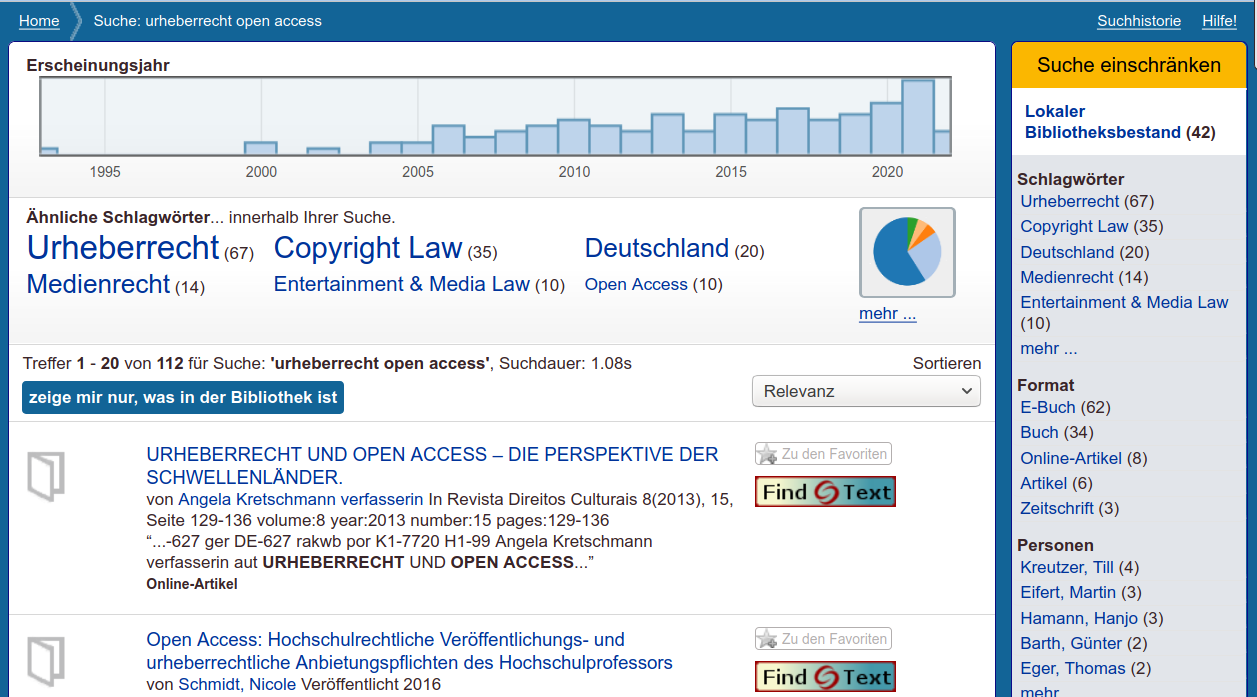
\includegraphics{media/vufind.png}

}

\caption{\label{fig-vufind}Beispiel eines Rechercheergebnisses in einem
Discovery-Interface}

\end{figure}%

\subsubsection{Bereitstellungsdienste}\label{bereitstellungsdienste}

Die Evaluationen früher Discovery-Systeme haben bereits gezeigt, dass
Informationen darüber, ob und wie ein gefundenes Medium zugänglich ist,
von zentraler Bedeutung sind. Diese Bereitstellungsdienste, auch
Delivery-Funktionen genannt, umfassen für physische und digitale Medien
jeweils unterschiedliche Aspekte.

Bereitstellungsdienste für physische Medien umfassen z.\,B.:

\begin{itemize}
\item
  Nachweise von Standorten, Ausleihbarkeit und aktuellem Ausleihstatus
\item
  Verlinkung zu Verbundkatalogen mit Fernleihmöglichkeiten
\item
  Verlinkung zu Fernleihe und Dokumentlieferdiensten
\item
  Möglichkeit zur Anfrage nach einer Digitalisierung oder Bereitstellung
  in einem Semesterapparat
\item
  Möglichkeit zur Abgabe eines Anschaffungsvorschlags
\end{itemize}

Bereitstellungsdienste für digitale Medien umfassen z.\,B.:

\begin{itemize}
\item
  idealerweise eine auf das jeweilige Nutzungsszenario angepasste
  Zugangs-URL
\item
  weitere Zugangs-URLs
\item
  Hinweise zur Nutzung elektronischer Medien, z.\,B.~zur Zugänglichkeit
  über VPN, notwendigen Readern, Digital Rights Management (DRM) etc.
\end{itemize}

Die Verfügbarkeit und Entleihbarkeit von physischen Medien, die der
Bibliothek gehören, werden über eine sogenannte Verfügbarkeitsrecherche,
die das Discovery-System im Hintergrund ausführt, ermittelt und
angezeigt. Diese Abfragen werden mittels
\hyperref[schnittstellen]{Schnittstellen} zu den Ausleihmodulen der BMS
durchgeführt. Diese Schnittstellen können proprietär oder offen sein.
Beispiele für herstellerunabhängige Schnittstellen sind die
\emph{Patrons Account Information API} (PAIA) als offene Schnittstelle
und das \emph{Session Initiation Protocol} (SIP2) als intern genutzter
Standard oder das NISO Circulation Interchange Protocol ({NCIP}).
Verschiedene Discovery-Systeme unterstützen diese oder andere
Schnittstellen zum Ausleihsystem in Form von sogenannten Treibern~--
beispielsweise unterstützt VuFind die Anbindung an FOLIO durch einen
eigenen FOLIO-Treiber.

Bei den digitalen Medien ist die größte Herausforderung, den jeweils
besten von in der Regel mehreren Zugangslinks für ein Medium zu
identifizieren und zur Anzeige zu bringen. Zur Ermittlung des besten
Zugangslinks sind in der Regel mehrere Prüfschritte erforderlich.
Idealerweise sind solche Prüfschritte konfigurierbar, allerdings ist
diese Funktion oftmals kein integraler Bestandteil von
Discovery-Systemen, sondern ein eigener Dienst. Ein Beispiel für einen
solchen separaten Dienst ist der Webdienst DAIA+ (Keßler 2018). Eine
andere Möglichkeit ist der Einsatz sogenannter Link Resolver. Beim Link
Resolving wird über die Metadaten ein Hyperlink zu Diensten der
Bibliothek ermittelt. Es wird vorrangig bei solchen Medien genutzt, die
nicht aus dem BMS der Bibliothek und E-Ressourcen stammen. Ein Verfahren
für das Link-Resolving ist \emph{Open-URL} (NISO-Standard
\href{https://www.niso.org/publications/z3988-2004-r2010}{\emph{Z39.88}}).

\subsection{Anreicherungsdienste}\label{anreicherungsdienste}

Die Ergänzung bibliotheksseitig erstellter Metadaten mit weiteren
Informationen erfolgte bereits in klassischen OPACs. Beispiele sind
gescannte Inhaltsverzeichnisse, Links auf Wikipedia-Artikel oder die
Integration von Buchcovern.

Zu den am häufigsten genutzten Anreicherungsdiensten gehören:

\begin{itemize}
\item
  Cover-Anzeigen
\item
  kontextabhängige Infoboxen mit Informationen aus Nachschlagewerken,
  z.\,B.~Autor*innenenportraits via \emph{Wikidata} oder \emph{GND,}
  Informationen aus Nachschlagewerken wie
  \emph{\href{https://www.munzinger.de/}{Munzinger}}
\item
  Empfehlungsdienste mit Hinweisen auf Literatur zum selben Thema
  (z.\,B.~\emph{BibTip}, \emph{bX})
\item
  Visualisierungen von Buchstandorten über Gebäudeinformationssysteme
  (z.\,B.~\emph{Mapongo, V:Scout})
\item
  Integration mit weiteren Diensten, z.\,B.~der Leseförderungs-App
  \emph{Antolin}
\end{itemize}

Grundsätzlich erlaubt die Systemarchitektur von Discovery-Systemen die
Integration von diesen und anderen Diensten über einschlägige
\hyperref[schnittstellen]{Schnittstellen}, sodass sich über die
gelisteten Dienste noch zahlreiche weitere Möglichkeiten ergeben.

\subsubsection{Personalisierung}\label{personalisierung}

Discovery-Systeme erlauben in der Regel eine Anmeldung in einem
persönlichen Bereich, der folgende Funktionalitäten umfassen kann:

\begin{itemize}
\item
  Einsicht in das Bibliothekskonto einschließlich der Möglichkeit zum
  Vormerken und Verlängern
\item
  Speicherung von Suchanfragen
\item
  Speicherung von Literaturlisten
\item
  Alerting-Dienste
\end{itemize}

Literaturlisten können alternativ dazu auch sitzungsbasiert gespeichert
werden. Dauerhaft gespeicherte Listen lassen sich auch veröffentlichen
und damit allgemein zugänglich machen, was auch die Präsentation von
Auswahllisten oder Semesterapparaten erlaubt.

Häufig können auch Suchanfragen gespeichert werden. Die Einrichtung von
Alerting-Diensten hilft den Nutzer*innen, sich mit wenig Aufwand über
neue Titel informieren zu lassen. Alerting-Dienste beinhalten das
regelmäßige (automatisierte) Absetzen einer Suchanfrage und das
Versenden von Informationen, wenn die Suchanfrage veränderte
Trefferlisten (in der Regel: neue Titel) liefert.

\subsubsection{Thematische
Sucheinstiege}\label{thematische-sucheinstiege}

Wie beschrieben bieten Trefferlisten mit Facetten und Empfehlungen zwar
durchaus die Möglichkeit, sich eine Treffermenge zu erschließen.
Allerdings fehlt Discovery-Systemen genau wie OPACs häufig die
Möglichkeit, eine systematische Suche durchzuführen. Teilweise wird ein
Browsing durch die klassifikatorische Inhaltserschließung angeboten,
jedoch fehlen vielen Datensätzen entsprechende Daten und das Browsing
bezieht sich dadurch jeweils nur auf Teilmenge des Suchraums. Aus diesem
Grund werden verschiedene Ansätze erprobt, um eine thematische Suche zu
ermöglichen. Hierzu zählen u.\,a.~folgende Projekte und Dienste:

\begin{itemize}
\item
  ein Nachbau der Browsing-Funktion an physischen Bücherregalen,
  z.\,B.~mit dem
  \href{https://nbn-resolving.org/urn:nbn:de:0290-opus-16040}{Blended
  Shelf}
\item
  die Nutzung von Normdaten zur Erstellung von Übersichtsseiten,
  z.\,B.~im \href{https://www.dla-marbach.de/katalog-beta/}{Katalog des
  Deutschen Literaturarchivs Marbach}
\item
  die Visualisierung von Treffermengen und den darin enthaltenen
  Zusammenhängen, wie zum Beispiel bei
  \href{https://openknowledgemaps.org/}{Open Knowledge Maps}, in einer
  \href{https://data.slub-dresden.de/}{prototypischen Installation der
  SLUB Dresden} oder mit dem kommerziellen Dienst \emph{Yewno}.
\end{itemize}

Diese Projekte und Dienste sind jedoch entweder noch relativ neu oder
wenig verbreitet und nicht oder nur mit Aufwänden nachnutzbar. Im Rahmen
einer strategischen Planung für den Einsatz eines Discovery-Systems muss
daher abgewogen werden, ob und wie ein thematischer Sucheinstieg
umgesetzt werden soll, zumal für eine Darstellung im Sinne einer
optimalen User Experience jeweils auch erhebliche Designaufwände
entstehen.

\section{Aufbau und Betrieb eines
Discovery-Systems}\label{aufbau-und-betrieb-eines-discovery-systems}

\subsection{Betriebsmodelle}\label{betriebsmodelle}

Der Betrieb eines Discovery-Systems stellt vergleichbare Anforderungen
und unterliegt ähnlichen Rahmenbedingungen wie der
\hyperref[technischer-betrieb]{Betrieb eines BMS}.

Im Inhousebetrieb werden alle Komponenten selbst durch die Bibliothek
betrieben. Damit sind in diesem Szenario die weitestgehenden Anpassungen
möglich. Ein vollständiger Inhouse-Betrieb erfolgt aufgrund der
benötigten Ressourcen allerdings meist nur bei kleinen oder sehr
speziellen Datenbeständen (z.\,B.~durch die Fachinformationsdienste)
oder in sehr großen Einrichtungen. Oft trifft man stattdessen auf
hybride Lösungen, in denen neben einem vergleichsweise kleinen eigenen
Index ein bestehender kommerzieller oder nicht-kommerzieller Index
genutzt wird.

In einem Hosting-Betrieb wird die gesamte Infrastruktur durch einen
Dienstleister bereitgestellt. Dabei erfolgt die Indexierung in der Regel
durch einheitliche Indexierungsverfahren, die von allen teilnehmenden
Bibliotheken gemeinsam genutzt werden. Bei diesen Lösungen werden alle
Daten in einen einheitlich aufgebauten, in einer Cloud gehosteten Index
eingespielt. Die Frontends sind nur eingeschränkt individualisierbar und
lassen sich ausschließlich durch Konfigurationen parametrisieren.
Zusatzfunktionen lassen sich über
\hyperref[schnittstellen]{Schnittstellen} anbinden. Wesentlicher Vorteil
dieser Systeme ist ein vergleichsweise geringer Wartungsaufwand, ihre
gute Skalierbarkeit und durch standardisierte Workflows ihre hohe
Betriebssicherheit. Als Hoster*innen von Discovery-Systemen treten
Bibliotheken, Verbünde und kommerzielle Anbieter auf.

Ein Spezialfall des Hostings ist die Nutzung von Cloud-Services externer
Anbieter*innen für den Betrieb von BMS und Discovery-Systemen. Mehrere
Hersteller*innen von BMS und Discovery-Systemen sind gleichzeitig
Betreiber*innen solcher Cloud-Lösungen. In diesen Fällen wird die
Software nicht mehr lizenziert, sondern über eine jährliche Pauschale
werden Nutzung, Update und Betrieb des jeweiligen Software-Systems
abgegolten.

Beim Hosting oder bei der Nutzung von Software, die in der Cloud
betrieben wird, erfolgt aus datenschutzrechtlicher Sicht eine
„\href{https://de.wikipedia.org/wiki/Datenverarbeitung_im_Auftrag}{Datenverarbeitung
im Auftrag}``. Die Verantwortung für Datenschutz und Datensicherheit
verbleibt damit bei der Bibliothek als Auftraggeberin (siehe
Kapitel~\ref{sec-datenschutz-externe}).

\subsection{Marktsituation}\label{marktsituation}

Die ersten Discovery-Systeme haben Bibliotheken selbst entwickelt, im
deutschsprachigen Raum z.\,B.~\emph{E-LIB} an der Staats- und
Universitätsbibliothek Bremen oder \emph{beluga} an der Staats- und
Universitätsbibliothek Hamburg. Seit Ende der 2000er Jahre gibt es auch
kommerzielle Systeme am Markt, entweder als Teil von BMS der neuesten
Generation oder auch als individuell lizenzierbare Systeme. Die
Open-Source-Lösung \emph{VuFind} ermöglicht es, verschiedene Suchindizes
unter einer Oberfläche nutzbar zu machen, sodass es eine relativ große
Vielfalt von Nutzungsszenarien gibt.

\subsubsection{Kommerzielle
Komplettsysteme}\label{kommerzielle-komplettsysteme}

Im Wesentlichen gibt es zwei Anbieter*innen von Komplettsystemen für
Discovery-Systeme

\begin{itemize}
\item
  ExLibris mit \emph{Primo} und \emph{Summon}
\item
  EBSCO mit \emph{Ebsco Discovery-Service}
\end{itemize}

Diese Systeme bieten eine fertige Lösung, in die lokale Bestandsdaten
und weitere lokale Metadaten integriert werden können. Für die Nutzung
fallen jährliche Lizenzgebühren sowie einmalige Implementierungskosten
an. Beide Systeme sind weit verbreitet und ausschließlich über die Cloud
der jeweiligen Hersteller*innen nutzbar. Diese sorgen für eine hohe
Verfügbarkeit und regelmäßige Softwarepflege. Individuell zu prüfen sind
vor einem möglichen Einsatz insbesondere folgende Fragen:

\begin{itemize}
\item
  Einbindung von Verfügbarkeitsinformationen
\item
  datenschutzrechtliche Fragen (Ort des Hostings,
  Verfahrensbeschreibungen)
\item
  Datenhoheit (siehe \hyperref[digitale-souveruxe4nituxe4t]{Digitale
  Souveränität})
\end{itemize}

Die Indizes dieser Systeme können separat lizenziert und beispielsweise
an \emph{\href{https://vufind.org/}{VuFind}}-Systeme angebunden werden.

Ein weiteres kommerzielles Discovery-System ist \emph{WorldCat
Discovery}, das allerdings die Nutzung von WorldCat als Suchindex
voraussetzt.

\subsubsection{Open-Source-Systeme}\label{open-source-systeme}

Unter den von Bibliotheken selbst entwickelten Discovery-Systemen sind
international \emph{VuFind} und
\emph{\href{http://projectblacklight.org/}{Blacklight}} am weitesten
verbreitet.

\emph{VuFind} basiert auf PHP und lässt sich an verschiedene
kommerzielle und frei verfügbare Komponenten wie Indizes und
Bibliotheksmanagementsysteme anbinden. In den deutschsprachigen Ländern
besteht eine lebendige Anwender*innengemeinschaft, die sich regelmäßig
trifft. Mit \emph{\href{https://www.qcovery.de/}{Qcovery}} und
\emph{\href{https://finc.info/}{finc}} gibt es zwei Subcommunities für
wissenschaftliche Bibliotheken, die sich die Aufgaben der Pflege und
Weiterentwicklung der Software unter sich aufteilen.

\emph{Blacklight} ist hauptsächlich im angloamerikanischen Raum
verbreitet, aber auch bei
\emph{\href{https://www.europeana.eu/}{Europeana}} Einsatz. Die Software
basiert auf Ruby on Rails.

Das von der VZG entwickelte System
\href{https://www.lukida.org/}{Lukida} spielt vor allem im Rahmen des
Index K10plus-Zentral eine Rolle und wird primär als {SaaS} angeboten.

\subsubsection{Indizes}\label{indizes}

Neben den kommerziellen Anbieter*innen bieten im Bereich
wissenschaftlicher Bibliotheken einige Verbundzentralen auf
Suchmaschinen-Technologie basierende Indizes an, teilweise für die
teilnehmenden Bibliotheken, teilweise auch darüber hinaus für die
nicht-kommerzielle Nutzung. Diese frei verfügbaren Indizes sind für
Bibliotheken, die ihre Bestandsdaten an einen Verbund liefern, eine
hervorragende Möglichkeit, um relativ kostengünstig an ein
Discovery-System zu kommen, da die Erstellung eines eigenen Index mit
hohen Investitionen verbunden ist. Metadatenkollektionen enthalten
z.\,B.~der ALBERT-Index des Kooperativen Bibliotheksverbundes
Berlin-Brandenburg sowie der Gemeinsame Verbündeindex für Bestandsdaten
aus allen wissenschaftlichen sowie vielen Spezial- und öffentlichen
Bibliotheken.

\subsection{Auswahl- und
Entscheidungsprozesse}\label{auswahl--und-entscheidungsprozesse}

Sofern ein Discovery-System nicht Teil des BMS ist, ist die Einführung
immer mit beträchtlichen Aufwänden verbunden, die aus initialen Kosten
für die Implementierung und laufenden Kosten für die Pflege bestehen.
Diese Kosten fallen unabhängig davon an, ob es sich um ein kommerzielles
oder ein Open-Source-System handelt. Sie richten sich nach
unterschiedlichen Kriterien und dürften im Bereich der initialen Kosten
im höheren vierstelligen Bereich liegen. Grundsätzlich sind die
Entscheidungsprozesse bei Auswahlentscheidungen mit denen für ein BMS
vergleichbar (vgl.~Abschnitt
\hyperref[marktanalyse-und-beschaffung]{Marktanalyse und Beschaffung}).

Allerdings müssen die strategischen Vorteile eines Discovery-Systems
sehr deutlich und auf den lokalen Bedarf hin herausgearbeitet werden. Es
hat sich als hilfreich erwiesen, dass Bibliotheken klar definieren, an
welche Zielgruppen sich ihr Discovery-System richtet und welche Aufgaben
es erfüllen soll. Es sollte auch geklärt werden, ob der klassische OPAC
nach Einführung eines Discovery-Systems überhaupt weiter angeboten
werden soll.

Auch der Zuschnitt der Suchräume sollte genau bedacht werden, vor allem
wenn über lokale Bestandsdaten hinaus eigene Metadatenkollektionen
(z.\,B.~aus institutionellen Repositorien) integriert und durch eigene
Suchfilter angesprochen werden sollen. Generell kann davon ausgegangen
werden, dass auf die initiale Implementierung eines Discovery-Systems
eine längere, oft mehrjährige Phase der Optimierung folgt, die
idealerweise konsequent auf die Usability und User Experience der
Hauptzielgruppen ausgerichtet ist (vgl.
Kapitel~\ref{sec-anforderungen}).

Die grundsätzliche Entscheidung für ein Discovery-System beinhaltet auch
einen Wechsel der Suchparadigmen. Die Einführung eines Discovery-Systems
kann nur dann sinnvoll erfolgen, wenn die Abkehr der Dualität von
Bestandsverzeichnis und Bibliografie sowie den traditionellen
Suchparadigmen strategisch erwünscht ist und von entsprechenden
Schulungen für das Bibliothekspersonal begleitet wird.

Wenn ein Discovery-System im Hosting genutzt werden soll, relativieren
sich obige Aussagen zur Flexibilität, da die Hosts in diesem Fall die
Möglichkeiten festlegen, die durch die Bibliotheken genutzt werden
können. In umgekehrter Weise verschieben sich die obigen Aussagen zur
Verantwortung für Betriebssicherheit und Verfügbarkeit.

\subsection{Monitoring und
Weiterentwicklung}\label{monitoring-und-weiterentwicklung}

Wie jedes IT-System brauchen Discovery-Systeme kontinuierliches
technisches Monitoring (vgl. Kapitel~\ref{sec-management}), ebenso wie
konzeptionelle Betreuung. Anders als der klassische Bibliothekskatalog
sind Discovery-Systeme angetreten, um sich konsequent nach dem
Informationsverhalten der Nutzer*innen auszurichten. Daraus ergibt sich,
dass sowohl die Implementierung als auch die weitere Entwicklung
möglichst kleinschrittig und unter Einbeziehung von Analysen der Nutzung
erfolgen sollten. Neben Methoden der Usability-Forschung (siehe
Abschnitt \hyperref[einbeziehung]{Wie beziehen wir unsere Nutzer*innen
ein?}) bietet sich als niedrigschwellige Methode vor allem die Analyse
von Logfiles an. So kann z.\,B.~mit der Software
\href{https://matomo.org/}{Matomo}, auch unter Berücksichtigung von
datenschutzrechtlichen Vorschriften, ermittelt werden, welche Anfragen
an ein System gestellt werden.

\section{Vergleich mit klassischen
Bibliothekskatalogen}\label{vergleich-mit-klassischen-bibliothekskatalogen}

Da Discovery-Systeme die Metadaten und Volltexte anders als die
klassischen OPACs aufbereiten, sind Suchstrategien und -ergebnisse in
beiden Systemen unterschiedlich.

Discovery-Systeme richten sich in der Regel an Benutzer*innen, die den
Umgang mit bibliografischen Recherchesystemen wie Katalogen und
Fachbibliografien nicht gewohnt sind und die mit den Nutzungsmustern
bedient werden sollen, die sie auch aus dem Web gewohnt sind.

Neben der Recherche nach bibliografischen Informationen sollen
Discovery-Systeme auch den Zugriff bzw.~die Bereitstellung von Medien
unterstützen. Dieser auch als \emph{Delivery} bezeichnete Prozess hat
sich bereits in der frühen Phase der Discovery-Systeme als zentrales
Element aus Sicht der Nutzer*innen herausgestellt. Die Anbindung an
Ausleihsysteme und Link Resolver ist daher ein wichtiges
Qualitätskriterium.

Neuere BMS wie \emph{FOLIO} und \emph{Alma} enthalten zum Teil gar
keinen klassischen OPAC mehr. Mit diesen Systemen muss daher immer ein
zusätzliches Discovery-System eingesetzt werden.

Ein Vorteil von Discovery-System gegenüber OPACs liegt in der
Auffindbarkeit von E-Ressourcen. Viele Bibliotheken erschließen
insbesondere im Open Access zugängliche E-Ressourcen nicht in vollem
Umfang in ihrem BMS. Daher sind im OPAC die E-Ressourcen nicht oder nur
eingeschränkt auffindbar. Wenn die Bibliothek ein Discovery-System
betreibt, können Metadaten zu E-Ressourcen über einen
\hyperref[etl-prozess]{ETL-Prozess} in den Index des Discovery-Systems
geladen werden. Voraussetzung dafür ist, dass den Metadaten mittels
Electronic Resource Management ({ERM}) entsprechende Nutzungslizenzen
zugeordnet sind.

\begin{longtable}[]{@{}
  >{\raggedright\arraybackslash}p{(\columnwidth - 4\tabcolsep) * \real{0.2000}}
  >{\raggedright\arraybackslash}p{(\columnwidth - 4\tabcolsep) * \real{0.3333}}
  >{\raggedright\arraybackslash}p{(\columnwidth - 4\tabcolsep) * \real{0.4556}}@{}}
\toprule\noalign{}
\begin{minipage}[b]{\linewidth}\raggedright
\end{minipage} & \begin{minipage}[b]{\linewidth}\raggedright
OPAC/Katalog
\end{minipage} & \begin{minipage}[b]{\linewidth}\raggedright
Discovery-System
\end{minipage} \\
\midrule\noalign{}
\endfirsthead
\toprule\noalign{}
\begin{minipage}[b]{\linewidth}\raggedright
\end{minipage} & \begin{minipage}[b]{\linewidth}\raggedright
OPAC/Katalog
\end{minipage} & \begin{minipage}[b]{\linewidth}\raggedright
Discovery-System
\end{minipage} \\
\midrule\noalign{}
\endhead
\bottomrule\noalign{}
\endlastfoot
Suchraum & nur lokaler Bestand, nur selbständige Werke & lokaler
Bestand, aber auch Verbunddaten, bibliografische Daten, Volltexte
etc. \\
Suchprinzip & exakte Suche, feldbasierte & Autovervollständigung,
Suchvorschläge, Facetten \\
Suchunterstützung & eher wenig & best match, natürlichsprachliche
Suche \\
Sortierung & nach Aktualität & nach Relevanz \\
Mehrwertdienste & Buchcover, Listen, Exportformate & Buchcover, Listen,
Exportformate \\
Metadaten & bibliothekarisches Schema, Hierarchien und Verweise &
„flache Version`` eines bibliothekarischen Schemas \\
\caption{Vergleich typischer Eigenschaften von OPAC/Katalog und
Discovery-System}\label{tbl-discovery-vs-opac}\tabularnewline
\end{longtable}

\section{Grenzen und Alternativen}\label{grenzen-und-alternativen}

Discovery-Systeme sind in der Regel nur einer von vielen Bausteinen in
der Prozesskette der Recherche, Bewertung und Beschaffung von Literatur
und spielen an unterschiedlichen Stellen eine Rolle. Sie helfen dabei,
Literatur zu entdecken und Zugangswege zu ermitteln und brechen die
traditionelle Grenze zwischen Katalog und Bibliografien durch einen
zentralen Sucheinstieg auf. Trotz dieser Stärken können die Systeme
nachgewiesene Medien nur eingeschränkt kontextualisieren und bewerten
und bleiben in der Praxis oft hinter den Erwartungen zurück (Christensen
2022). Je nach Anwendung spielen daher alternative Systeme weiterhin
eine Rolle:

\begin{itemize}
\item
  Komplexe bibliografische Angaben, zum Beispiel zum Erscheinungsverlauf
  von Zeitschriften oder mehrbändigen Werken, oder die Suche nach
  Signaturen lassen sich möglicherweise schneller über herkömmliche
  bibliothekarische Instrumente beziehungsweise Spezialdatenbanken wie
  die des BMS ermitteln.
\item
  Zum Entdecken von Literatur eignen sich auch allgemeine Suchmaschinen
  oder spezielle Academic Search Engines wie Google Scholar sowie
  gänzlich andere Wege wie bestehende Literaturverzeichnisse,
  Empfehlungslisten auf Lernplattformen und Webshops.
\end{itemize}

Insbesondere Webshops haben im Vergleich zu Discovery-Systemen sehr
personalisierte Such- und Empfehlungsdienste, die jedoch auf einer
intensiven Auswertung des jeweiligen Nutzungsverhaltens basieren. Die
Verwendung dieser Daten zur Personalisierung ist auch in
Discovery-Systemen denkbar, wird aber aus Datenschutz- und
Neutralitätsgründen grundsätzlich eher abgelehnt.

Eine vergleichsweise neue Herangehensweise insbesondere an das
entdeckende Suchen bieten Wissensgraphen (\emph{knowledge graphs}), die
die vielfältigen Beziehungen zwischen Dokumenten und damit verknüpften
Elementen darstellen und visualisieren. Die Anforderungen an die
Qualität der so aufbereiteten Daten sind jedoch ungleich höher.
Entsprechende Systeme existieren bereits in ausgewählten Bereichen,
z.\,B.~die Plattform \emph{\href{https://sonar.fh-potsdam.de/}{SoNAR}}
zur historischen Netzwerkanalyse. Ein ernstzunehmendes Beispiel für
einen allgemeinen Wissensgraphen ist die Datenbank Wikidata mit ihren
bibliografischen Inhalten \emph{WikiCite} und dem dazu gehörigen
Browsing-Interface \emph{\href{https://scholia.toolforge.org/}{Scholia}}
(siehe Abbildung Abbildung~\ref{fig-scholia}).

\begin{figure}

\centering{

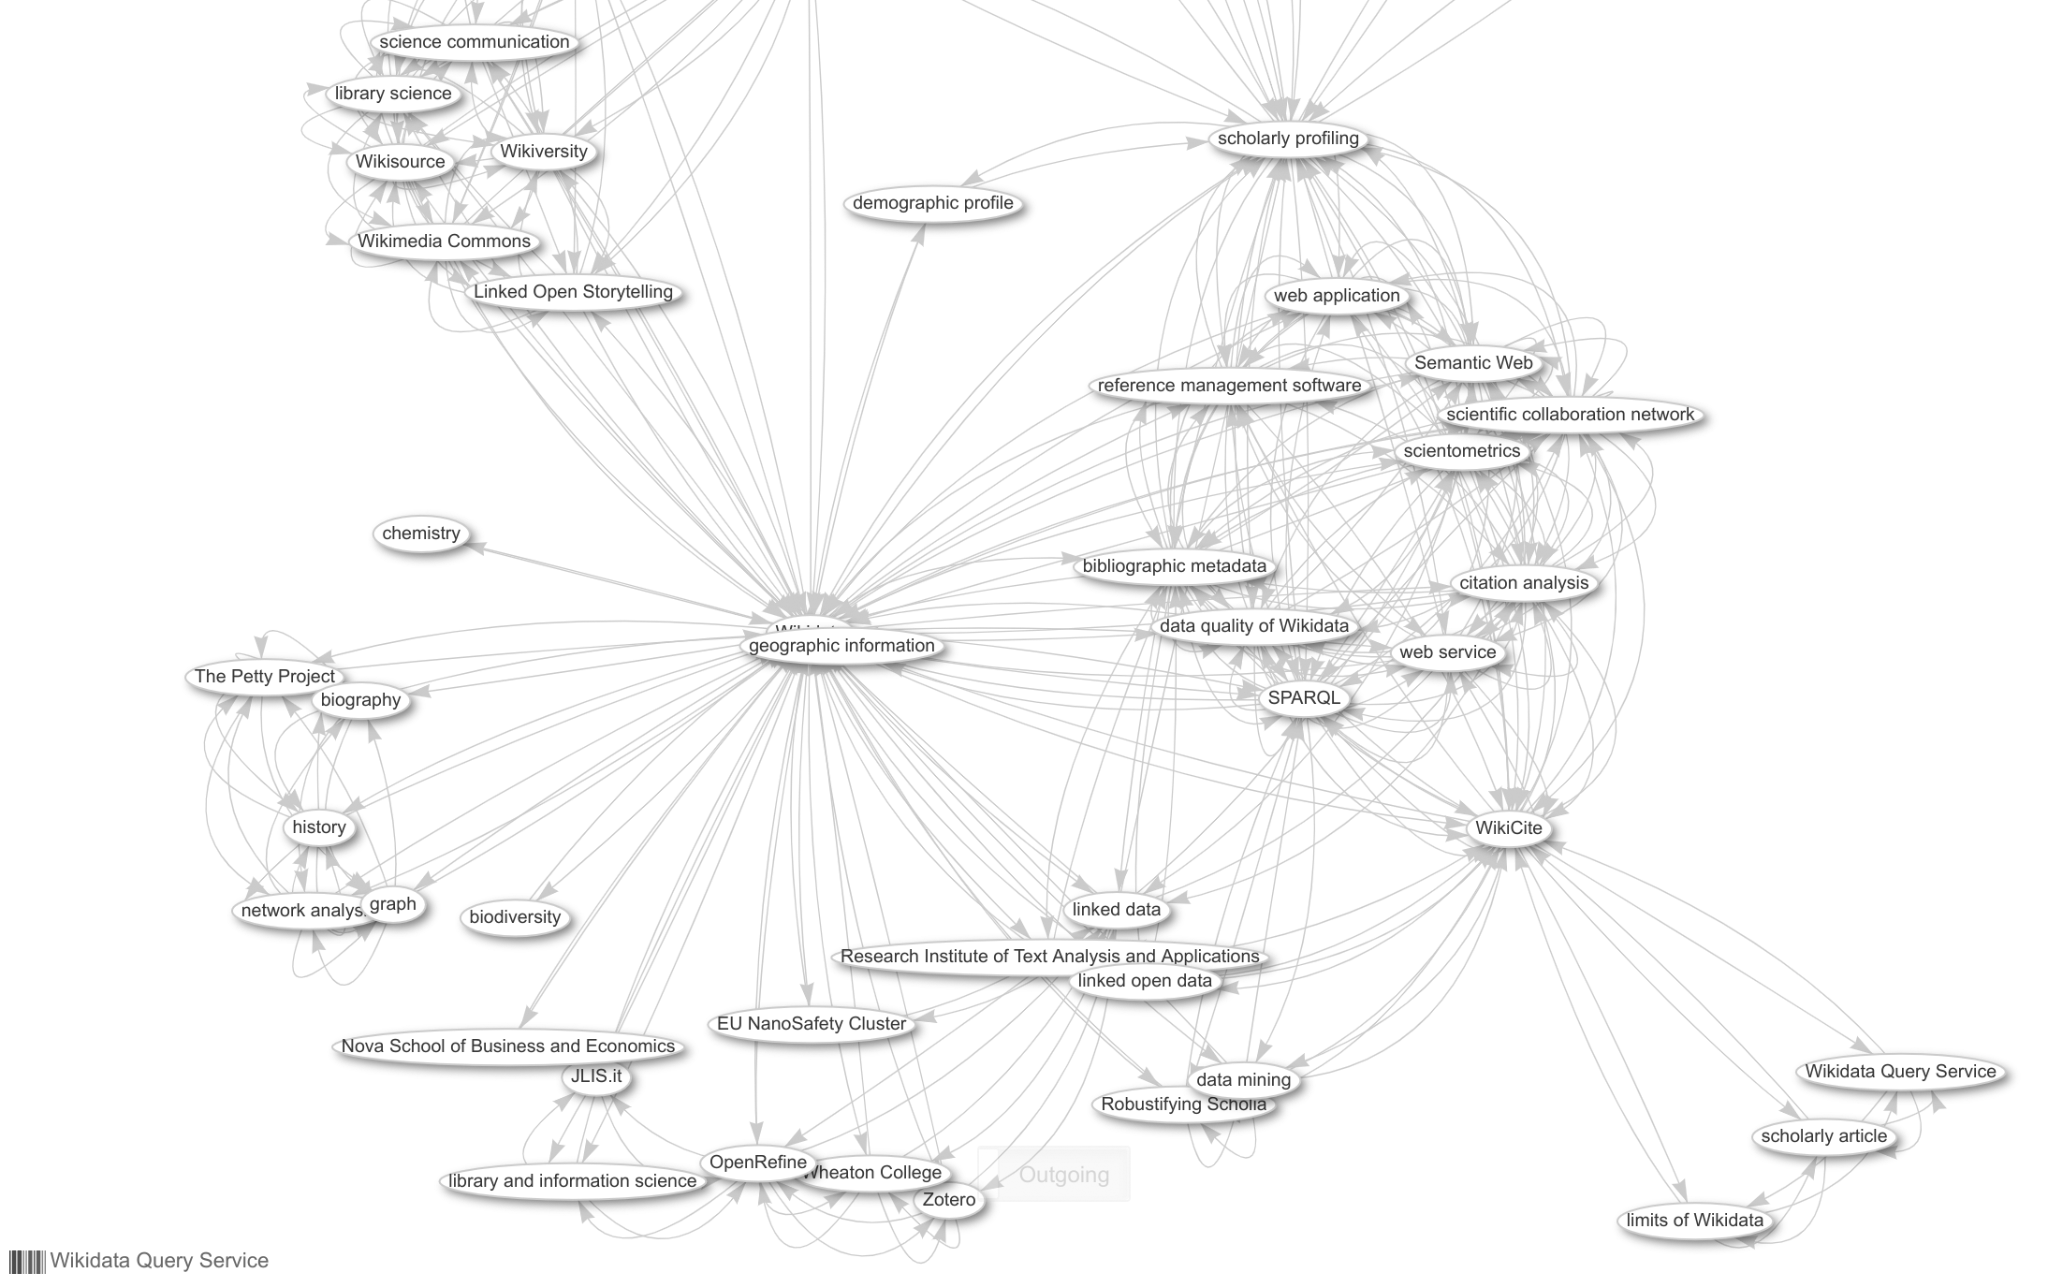
\includegraphics{media/scholia.png}

}

\caption{\label{fig-scholia}Thematisches Netzwerk von Publikationen in
und über Scholia}

\end{figure}%

Grundsätzlich gilt, dass die Grenzen zwischen Discovery-Systemen und
Alternativen in der Praxis fließend sind und dass Discovery-Systeme
perspektivisch um Funktionen anderer Systeme erweitert werden können und
sollten.

\section{Zusammenfassung \& Ausblick}\label{zusammenfassung-ausblick-1}

Discovery-Systeme kommen den Erwartungen von Benutzer*innen an das
Suchen und die Erreichbarkeit von Medien entgegen. Insbesondere
Bibliotheken, die kein Bibliotheksmanagement-System
(Kapitel~\ref{sec-bibliotheksmanagementsysteme}) verwenden, das bereits
eine Discovery-Oberfläche enthält, müssen sich daher oft und mit hoher
Priorität damit auseinandersetzen, wie Informationen über den eigenen
Bestand durch ein Discovery-System besser zugänglich gemacht werden.
Dies eröffnet Fragen nach möglichen
\hyperref[betriebsmodelle]{Betriebsmodellen}, gegebenenfalls des
\hyperref[change-management]{Change Management}, bis hin zum
kontinuierlichen \hyperref[monitoring-und-weiterentwicklung]{Monitoring}
und der Weiterentwicklung solcher Dienste.

\bookmarksetup{startatroot}

\chapter{Digitalisierung}\label{sec-digitalisierung}

\begin{tcolorbox}[enhanced jigsaw, leftrule=.75mm, toprule=.15mm, left=2mm, opacityback=0, arc=.35mm, colback=white, breakable, colframe=quarto-callout-note-color-frame, rightrule=.15mm, bottomrule=.15mm]
\begin{minipage}[t]{5.5mm}
\textcolor{quarto-callout-note-color}{\faInfo}
\end{minipage}%
\begin{minipage}[t]{\textwidth - 5.5mm}

\vspace{-3mm}\textbf{Zusammenfassung}\vspace{3mm}

Neben der reinen Bewahrung von Kulturgütern stellt sich Bibliotheken und
anderen Kultureinrichtungen die Herausforderung, diese weltweit im Netz
zugänglich zu machen. Die Digitalisierung von Kulturgut erfordert
verschiedene Prozesse und Tools, die in diesem Kapitel vorgestellt
werden.

\end{minipage}%
\end{tcolorbox}

\section{Grundlagen}\label{grundlagen}

Digitalisierung ist zu einer zentralen Aufgabe an vielen Bibliotheken
geworden. Über die Jahren haben sich für diese Aufgabe technische und
organisatorische Standards und Workflows entwickelt und konsolidiert. So
existieren inzwischen zahlreiche Softwaresysteme wie
z.\,B.~Workflow-Managementsysteme.

\subsection{Ziele der Digitalisierung}\label{ziele-der-digitalisierung}

Zu den Zielen der Digitalisierung zählen vor allem die Bestandserhaltung
und Bestandsentwicklung. Durch die digitale Verfügbarmachung soll der
Kundennutzen erhöht werden, indem Teilhabe und Zugang zu den Objekten
erleichtert werden. Deshalb gibt es einen engen Bezug zu Themen wie Open
Access oder Open Science. Durch eine erhöhte Sichtbarkeit der
Institutionen bzw.~einzelner Objekte und Sammlungszusammenhängen wird
die Steigerung der institutionellen Relevanz angestrebt.

\subsection{Begriffsbestimmung}\label{begriffsbestimmung}

\textbf{Digitalisierung} steht in diesem Kapitel für die Überführung von
materiellen Kulturgütern in digitale Formate. Bibliotheken und andere
kulturbewahrende Institutionen nehmen sich für die Digitalisierung
sowohl Schriftgut (Bücher, Handschriften, Nachlässe) als auch
audiovisuelle Medien und andere Objekttypen vor. Dabei wird oft auch von
\textbf{Retrodigitalisierung} oder \textbf{Bestandsdigitalisierung}
gesprochen, wenn die Objekte nicht originär digital sind
(„born-digital``), sondern bereits physische vorlagen und erst später
digitalisiert werden.

\subsection{Geschichte}\label{geschichte}

Als Vorläufer der Digitalisierung kann die Mikroverfilmung betrachtet
werden, bei der bereits seit dem 19. Jahrhundert analoge Dokumente mit
dem Ziel der Langzeiterhaltung, der Vervielfältigung oder als
platzsparender Ersatz für Originale in ein anderes analoges Format
transformiert wurden. Die Überführung in digitale Formate begann in den
1990er-Jahren. Das Ziel war hier zunächst vor allem die weltweite
Zugänglichmachung von besonderen Werken oder Beständen für die
wissenschaftliche Nutzung. Waren es zunächst vor allem bedeutende
Druckwerke des 16., 17. und 18. Jahrhunderts, die digitalisiert wurden,
hat sich der Fokus der Digitalisierung auch zeitlich, thematisch und
formal sehr erweitert.

In Deutschland war und ist die Deutsche Forschungsgemeinschaft (DFG) ein
wesentlicher Akteur, der durch Projektförderung erhebliche Impulse für
die großflächige Retrodigitalisierung gegeben hat. Gleichzeitig sorgten
die in geförderten Projekten verbindlichen
\href{https://zenodo.org/records/7435724}{DFG-Praxisregeln}, die auch in
anderen Projekten oft angewendet werden, für ein hohes Maß an
Einheitlichkeit und Interoperabilität zwischen verschiedenen Beständen.
Neben technischen Parametern für den
\hyperref[scanner-und-scanverfahren]{Scan-Prozess} (Auflösung, Farbtiefe
u.\,a.) und Speicherformaten (TIFF unkomprimierte Master-Images) werden
dort Standards zur \hyperref[metadaten-und-schnittstellen]{Speicherung
von Metadaten} festgelegt, die von der Library of Congress entwickelt
wurden und weiter gepflegt werden. Die DFG hat darüber hinaus mit dem
\href{https://dfg-viewer.de/}{DFG-Viewer} einen Minimalstandard in der
\hyperref[pruxe4sentieren]{Objektpräsentation} entwickeln lassen. Zu den
Standards der DFG-Förderung gehört auch, dass jedes Werk nur einmal
digitalisiert werden soll.

Eine weitere große Digitalisierungsinitiative ging und geht von Google
aus, die weltweit und in Deutschland insbesondere bei der Bayerischen
Staatsbibliothek in großem Umfang alte Druckwerke digitalisieren (Google
Books).

Ergänzend digitalisieren, veröffentlichen, erschließen und editieren
private Akteure digitale Kulturgüter~-- Akteure in Wikimedia-, Open
Data- und Open-Science-Gemeinschaften, oder sie arbeiten ehrenamtlich in
einschlägigen bibliothekarischen Projekten mit.

\subsection{Status quo}\label{status-quo}

Zahlreiche Bibliotheken mit umfangreichen unikalen Beständen haben sich
auf den Weg gemacht, Retrodigitalisierung als festes Arbeitsfeld in die
eigene Organisation aufzunehmen. Für die Unterstützung der Prozesse und
für die Präsentation der Ergebnisse im Web haben sich unterschiedliche
Softwarelösungen etabliert, zu denen aktive Anwendergemeinschaften
gehören. Zusammen mit den geklärten Standards ist ein Rahmen geschaffen,
in dem diese Bibliotheken kontinuierlich neue Digitalisierungsprojekte
starten. Größere Häuser öffnen zum Teil ihre Infrastruktur anderen
kleineren Einrichtungen in Landesprogrammen wie z.\,B.~in
\href{https://www.slub-dresden.de/ueber-uns/projekte/landesdigitalisierungsprogramm}{Sachsen}
oder
\href{https://www.sub.uni-hamburg.de/bibliotheken/projekte-der-stabi/hamburger-kulturgut-im-netz-hakin.html}{Hamburg}.
In Berlin unterstützt die Arbeitsstelle
\href{https://www.digis-berlin.de/digis/}{digiS} mit einem jährlichen
\href{https://www.digis-berlin.de/foerderprogramm/info/}{Förderprogramm}
seit 2012 Digitalisierungsprojekte in unterschiedlichen technischen
Umgebungen~-- um nur einige Beispiele aus der heterogenen föderalen
Struktur herauszugreifen.

\subsection{Ausblick}\label{ausblick}

Neben der reinen bildhaften Digitalisierung wird von Forschenden
zunehmend auch eine Erstellung und Bereitstellung von Volltexten
erwartet. Diese kann entweder über einfache Text-Bild-Zuordnung oder
auch mit aufwändiger semantischer Auszeichnung erfolgen. Die von der DFG
geförderte Initiative OCR-D erstellt Werkzeuge und Infrastrukturen, um
für die Werke des 16., 17. und 18. Jahrhunderts, aber auch für viele
weitere Digitalisate eine effiziente und alltagstaugliche
Volltexterstellung zu ermöglichen.

Außer Druckwerken und Handschriften werden zunehmend weitere Medien und
Objekte digitalisiert. Das sind nicht nur einschlägige Textdokumente aus
Bibliotheken und Archiven, sondern auch Objekte aus Sammlungen und
Museen, die teilweise auch in 3D digitalisiert werden, und audiovisuelle
Medien. Außerdem wird versucht, zusätzliche Attribute der materiellen
Objekte zu erfassen (z.\,B.~Strukturerkennung, Kontextinformationen).

Zudem werden sich GLAM-Einrichtungen auch immer stärker des Bedarfes
bewusst, Digitalisate auch jenseits eigener Portale auffindbar und
nutzbar zu machen (siehe
\hyperref[digitalisierung-als-beitrag-zur-open-glam-bewegung]{Digitalisierung
als Beitrag zur Open GLAM-Bewegung}).

\section{Prozesse}\label{prozesse}

Die Digitalisierung von Kulturgütern gliedert sich in mehrere
Prozessschritte. Es haben sich dabei einrichtungsübergreifend ähnliche
Prozessketten etabliert, zu deren Unterstützung
\hyperref[workflowmanagementsysteme]{Workflowmanagementsysteme} (WMS)
entwickelt wurden und die Projektsteuerung erleichtern.

\begin{figure}

\centering{


\includegraphics{index_files/mediabag/media/prozesse-digitalisierung.pdf}

}

\caption{\label{fig-prozess-digitalisierung}Prozessschritte im
Digitalisierungsprozess}

\end{figure}%

Als Ausgangspunkt jedes Digitalisierungs-Vorhabens ist eine gründliche
Planung der Arbeitsschritte unverzichtbar. Dabei sind die lokalen
Rahmenbedingungen und die Infrastruktur der digitalisierenden
Einrichtung ebenso zu berücksichtigen wie die konkreten Ziele, die zu
erzeugenden Formate und Ergebnisse sowie die Verknüpfungen zu externen
datenverarbeitenden Systemen. Die
\href{https://doi.org/10.5281/zenodo.7435724}{DFG-Praxisregeln} geben
wichtige Hinweise, was bei den Prozessen beachtet werden sollte. WMS
können diese Schritte steuern und teilweise auch automatisieren.

Für die Planung von Zeitungsdigitalisierung sollte im Vorwege besonders
genau auf die Einzelschritte im Prozess geschaut werden oder kollegiale
Beratung aus anderen Häusern eingeholt werden, um angesichts der Massen
an Material den effizientesten Weg bei der Erschließung zu finden, evtl.
Dienstleister optimal einzubinden und alle Möglichkeiten von
Automatisierung auszuschöpfen.

\subsection{Vorbereiten: Auswahl von
Objekten}\label{vorbereiten-auswahl-von-objekten}

Eine sinnvolle Auswahl zu digitalisierender Objekte hängt von Faktoren
ab, deren Wichtigkeit gegeneinander abzuwägen ist. Dazu zählen
beispielsweise

\begin{itemize}
\item
  die bestehenden Kapazitäten: verfügbare Scanverfahren, Arbeitsplätze,
  personelle Verfügbarkeiten,
\item
  die technischen Ausstattung: Scanner, Speicherkapazität, Anbindung an
  eine Langzeitarchivierung
\item
  zeitliche Faktoren: Projektlaufzeit, Förderbedingungen, Anlässe,
\item
  Digitalisierungswürdigkeit: Einzigartigkeit, Nachfrage
\item
  Erhaltungszustand: Dringlichkeit, Machbarkeit
\item
  existierende Vorarbeiten: vorhandene Metadaten, Vervollständigung
  bereits angefangener Vorhaben
\end{itemize}

Die Prioritäten für die eigene Bestandsdigitalisierung sollten immer
wieder überprüft werden, wenn sich die genannten Faktoren ändern.

Nach der Auswahl von zu digitalisierenden Objekten folgen weitere
vorbereitende Schritte. Dazu gehören z.\,B.

\begin{itemize}
\item
  das Ausheben der Werke aus dem Bestand
\item
  das Überprüfen und ggf.~das Herstellen der
  Digitalisierungstauglichkeit
\item
  das Anlegen von Vorgängen im Workflowmanagementsystem
\item
  das Erzeugen von Laufzetteln
\item
  die Vorbereitung von Übergaben physischer Objekte an etwaige
  Scandienstleister
\end{itemize}

\subsection{Digitalisieren}\label{digitalisieren}

Die Entscheidung für das oder die am besten geeigneten
Digitalisierungsverfahren ist individuell am Objekt zu treffen und hängt
von verschiedenen Faktoren ab, wie der Art des Objekts, der gewünschten
Genauigkeit und den verfügbaren Ressourcen.

\subsubsection{2D-Objekte}\label{d-objekte}

Für das Scannen von 2D-Objekten („Flachware``) hat sich als Zielformat
der Bilddigitalisierung unkomprimiertes
\href{https://de.wikipedia.org/wiki/Tagged_Image_File_Format}{TIFF}
etabliert. Es werden mit Aufsichtscannern oder fotografischen
Reproständen Einzelseiten aufgenommen und vom Bildausschnitt her wird
mit schwarzem Rand digitalisiert. Verschiedene Auflösungen („Derivate``)
für die Webpräsentation werden nachgelagert erzeugt oder dynamisch von
einem Bildserver zur Verfügung gestellt.

Für die verschiedenen Digitalisierungsvorhaben bilden die
\href{https://doi.org/10.5281/zenodo.7435724}{DFG-Praxisregeln} für die
Auflösung, den Farbraum und andere technische Parameter eine gute
Orientierungshilfe. Für die Beurteilung und Sicherstellung der
objektiven Bildqualität haben sich zudem Digitalisierungsstandards
etabliert, die mittlerweile auch von Scannerherstellern und
Scandienstleistern berücksichtigt werden. Erwähnenswert sind hier vor
allem
\href{https://www.metamorfoze.nl/english/digitization}{Metamorfoze} und
der daraus hervorgegangene
\href{https://www.iso.org/standard/64220.html}{ISO-19263 Standard} .

Bei der Zeitungsdigitalisierung ist im Interesse der Forschung die
Erzeugung von Volltexten nach der Digitalisierung ein wichtiges Ziel.
Diese Perspektive bedingt im Hinblick auf die Qualität der Texterkennung
(OCR) eine Präferenz für eine Digitalisierung vom Original gegenüber
einer Digitalisierung vom Mikrofilm.

\subsubsection{3D-Objekte}\label{d-objekte-1}

Mittlerweile haben einige Bibliotheken angefangen, über flache,
zweidimensionale Informationen hinaus auch die Tiefe und
Mehrdimensionalität des kulturellen Erbes und Wissens innerhalb ihrer
Bestände zu erfassen. Bibliotheksbestände sind häufig heterogen und
ergeben sich aus einer fortgesetzten Sammlungsgeschichte, sodass auch
spezielle dreidimensionale Objekte, wie Globen, Spiel- oder PopUp-Bücher
oder historische Objekte des Buchdrucks wie Lettern, Teil eines
Bestandes sein können. In diesen Fällen hat sich eine Digitalisierung in
allen drei Dimensionen als ein entscheidendes Werkzeug erwiesen, um die
Mehrdimensionalität in digitale Formate zu übertragen und um über
Inhalte hinaus den Zustand und Details als Kulturerbeobjekte
wiederzugeben. Dies betrifft ebenso seltene Bücher und Manuskripte mit
einzigartigen oder kunstvollen Bindungen. Um die drei Dimensionen
angemessen abzubilden, sind
\hyperref[scanner-und-scanverfahren]{spezielle Erfassungsmethoden}
notwendig.

\subsubsection{AV-Medien}\label{av-medien}

Bibliotheken und andere GLAM-Einrichtungen archivieren häufig auch
analoge audiovisuelle Medien. Für die Digitalisierung der
unterschiedlichen Quellen (z.\,B.~Magnettonbänder, Film von 8~mm bis
35~mm, Selbstschnittplatten, Videobänder) werden im Falle einer
Massendigitalisierung zumeist externe Dienstleister beauftragt, sodass
die Herausforderungen hier in erster Linie in der inhaltlichen
Erschließung und der Erhaltung des originalen Materials liegen.

\textbf{Für alle Materialarten gilt:} Eigene Scanner sind nur
erforderlich, wenn der Scanprozess nicht an einen Dienstleister
ausgelagert werden soll oder kann. Nach der Auswahl geeigneter Geräte
(am besten nach Beratung durch erfahrene Einrichtungen) empfiehlt sich
eine Teststellung, bei der diese unter Realbedingungen erprobt werden
können.

\subsection{Erschließen}\label{erschlieuxdfen}

\subsubsection{Erschließen von
Metadaten}\label{erschlieuxdfen-von-metadaten}

Erschließen bedeutet das Zusammentragen von allen verfügbaren
Informationen zu einem Objekt und die Codierung in Form von Metadaten
(Kapitel~\ref{sec-metadaten}). Im Kontext der Digitalisierung sind drei
Arten von Metadaten (Kapitel~\ref{sec-arten-von-metadaten}) besonders
relevant:

\begin{itemize}
\item
  \textbf{Administrative Metadaten} mit Informationen zu Herkunft,
  Erhaltungszustand, technische Merkmale, Rechteinformationen.
\item
  \textbf{Deskriptive Metadaten} zur bibliografischen Beschreibung des
  Objektes.
\item
  \textbf{Strukturelle Metadaten} für Gliederungselemente wie
  z.\,B.~Kapitel in Texten, Segmente in 3D-Objekten, Frames in Filmen.
\end{itemize}

Bibliografische Basisdaten wie auch strukturelle Metadaten können in
einem WMS entweder importiert oder manuell erfasst werden. Viele der
Systeme sind dafür individuell konfigurierbar und können je nach Art des
Projektes angepasst werden. Wichtige Metadaten sind
\hyperref[identifikatoren]{Identifikatoren} (URN, DOI, PURL \ldots) und
deren Generierung. Für die Strukturierung von Textdokumenten ist das
\href{https://dfg-viewer.de/strukturdatenset}{Stukturdatenset für den
DFG-Viewer} ein praxistauglicher Referenzrahmen.

Um die Nachnutzung der digitalisierten Objekte zweifelsfrei zu
kennzeichnen, gehören Informationen zur Lizenzierung in die
administrativen Metadaten. Dafür hat eine Expertengruppe innerhalb von
DINI detaillierte
\href{https://wiki.dnb.de/pages/viewpage.action?pageId=217533652}{Empfehlungen
für Rechteinformationen in Metadaten} aufgestellt.

Strategien für das Crowdsourcing von Erschließungsarbeiten in offenen
Informationsinfrastrukturen wie dem Wikiversum ermöglichen potenziell
zusätzliche Mehrwerte, auch im Nachhinein und durch Dritte.

\subsubsection{Zusätzliche inhaltliche Erschließung durch Volltexte und
Annotationen}\label{zusuxe4tzliche-inhaltliche-erschlieuxdfung-durch-volltexte-und-annotationen}

Erschließung endet nicht bei der Zuordnung von Metadaten. Ziel der
Erschließung ist auch eine Abbildung des Werkes in nachnutzbarer Form.
Bei Textdokumenten ist das die Generierung von Volltexten. Für die
Auswahl eines Verfahrens und deren Parametrisierung sind Eigenschaften
der Vorlage (Schriftart, Layout, Sprache, Papier- und Druckqualität
u.\,a.) sowie die benötigte Qualität der Volltexte entscheidend.

Waren anfangs vor allem kommerzielle OCR-Werkzeuge dominierend (z.\,B.
\href{https://de.wikipedia.org/wiki/ABBYY}{ABBYY}), haben sich
mittlerweile einige Open-Source-Projekte (z.\,B.
\href{https://de.wikipedia.org/wiki/Tesseract_(Software)}{Tesseract})
entwickelt, die qualitativ vergleichbare oder bessere Ergebnisse
erzeugen können. Dank neuer technologischer Ansätze sind auch Lösungen
für handschriftliche Dokumente verfügbar (z.\,B.
\href{https://www.ocr4all.org/about/ocr4all}{OCR4all}). Mit Förderung
durch die DFG arbeitet die Initiative OCR-D an einem frei nutzbaren
Workflow, der neben der eigentlichen Volltexterkennung weitere Schritte
(z.\,B.~automatische Layouterkennung) einbindet, die die Qualität der
Erschließung verbessern.

Die Generierung von Volltexten kann als (automatischer) Prozessschritt
im \hyperref[workflowmanagementsysteme]{Workflowmanagementsystem}
eingebunden werden. Die Ergebnisse werden in der Regel in
\hyperref[metadaten-und-schnittstellen]{standardisierten Datenformaten}
geliefert und können dann in Präsentationssystemen z.\,B.~für die
Volltextsuche genutzt oder zum Download angeboten werden.

Neben Volltexten können je nach Kontext auch Annotationen als weiteres
Element der Erschließung eine Rolle spielen, die aber in der Regel nicht
im Digitalisierungsprozess, sondern erst im Nachhinein entstehen.

\subsection{Präsentieren}\label{pruxe4sentieren}

Die Präsentation von digitalisierten Objekten und den dazugehörigen
Metadaten im Web ist ein wesentliches Ziel der
Digitalisierungs-Aktivitäten.

Die Präsentation der digitalisierten Objekte hängt von der Art von
Objekten und beabsichtigten Nutzungsszenarien ab und erfordert eigene
Werkzeuge, die unabhängig von dem genutzten Workflowmanagementsystem
ausgewählt und konfiguriert werden. Basis für Präsentationslösungen sind
die im Workflow erzeugten standardisierten XML-Files (METS/MODS).

Funktional wird von einer Präsentationslösung eine konfigurierbare
Rechercheumgebung für Metadaten und Volltexte erwartet. Bei der
Präsentation des einzelnen Objektes werden die Strukturdaten zusammen
mit den dazu erfassten Metadaten als Inhaltsverzeichnis angeboten und es
werden zur Arbeit mit den Scans Bildwerkzeuge erwartet (z.\,B.~Zoomen,
Rotieren, Thumbnail-Übersicht). Zunehmend wichtige Funktionen sind
Downloadangebote oder die Bereitstellung von IIIF-Manifesten zur
Weiternutzung in anderen Viewern.

Mit dem \href{http://dfg-viewer.de/}{DFG-Viewer} existiert eine
Minimallösung für die Anzeige von Digitalisaten, die aus dem Katalog
verlinkt werden kann. Für eine umfassendere Präsentation von
Digitalisaten entscheiden sich Einrichtungen für eine Integration der
Digitalisate in ein existierendes Repositorium oder für den Aufbau von
Webangeboten mit speziellen Werkzeugen für Digitalisate wie z.\,B.
\emph{Kitodo.Presentation}. Ein wichtiges Element für mehr Sichtbarkeit
der eigenen Digitalisierungsaktivitäten ist eine Datenlieferung an die
Deutsche Digitale Bibliothek.

Zunehmend relevanter wird die Suche nach Lösungen für eine Präsentation
von rechtebehafteten Materialien für eingeschränkte Personenkreise.
\hyperref[repositorien-fuxfcr-forschungsergebnisse]{Repositorien} haben
hier in der Regel schon anpassbare Lösungen. Bei der Präsentation von
Digitalisaten existieren prototypische oder an Institutionen individuell
angepasste technische Lösungen. Standards für die Beschreibung von
Zugriffsrechten in den Metadaten oder generische Präsentationslösungen
auf Basis dieser Metadaten befinden sich noch im Abstimmungsprozess oder
der Entwicklung.

Wikimedia Commons kann darüber hinaus als Medienspeicher fungieren. Von
dort werden digitalisierte Objekte und „born digital``-Dokumente in
Wikipedia und andere Webseiten eingebettet. Die Erschließung mit
strukturierten Daten erfolgt mittels Wikidata (siehe
\hyperref[digitalisierung-als-beitrag-zur-open-glam-bewegung]{Digitalisierung
als Beitrag zur Open GLAM-Bewegung}).

\section{Werkzeuge}\label{werkzeuge-1}

\subsection{Scanner und Scanverfahren}\label{scanner-und-scanverfahren}

\subsubsection{2D}\label{d}

Scanner und ihre Verfahren lassen sich grundlegend nach der Eigenschaft
ihrer zu scannenden Objekte und der Zielsetzung des Scan-Ergebnisses
unterscheiden.

Im Bereich des 2D-Scans unterstützen z.\,B.~spezielle Buchscanner den
Scanprozess im Rahmen der Digitalisierung effizient und für das zu
digitalisierende Material auf schonende Weise. Das sind in der Regel
Auflichtscanner oder fotografische Systeme, bei denen das Material von
oben abgelichtet wird. Je nach Art und Zustand des Materials können
dabei Buchwippen bzw.~-wiegen mit verschiedenen Winkeln oder Glasplatten
eingesetzt werden. Roboter können das automatische Umblättern der Seiten
erledigen, sind dabei aber für empfindliche Bestände weniger schonend.
Berührungslose Scanner sind vor allem für Handschriften vorgesehen.

\begin{figure}

\centering{

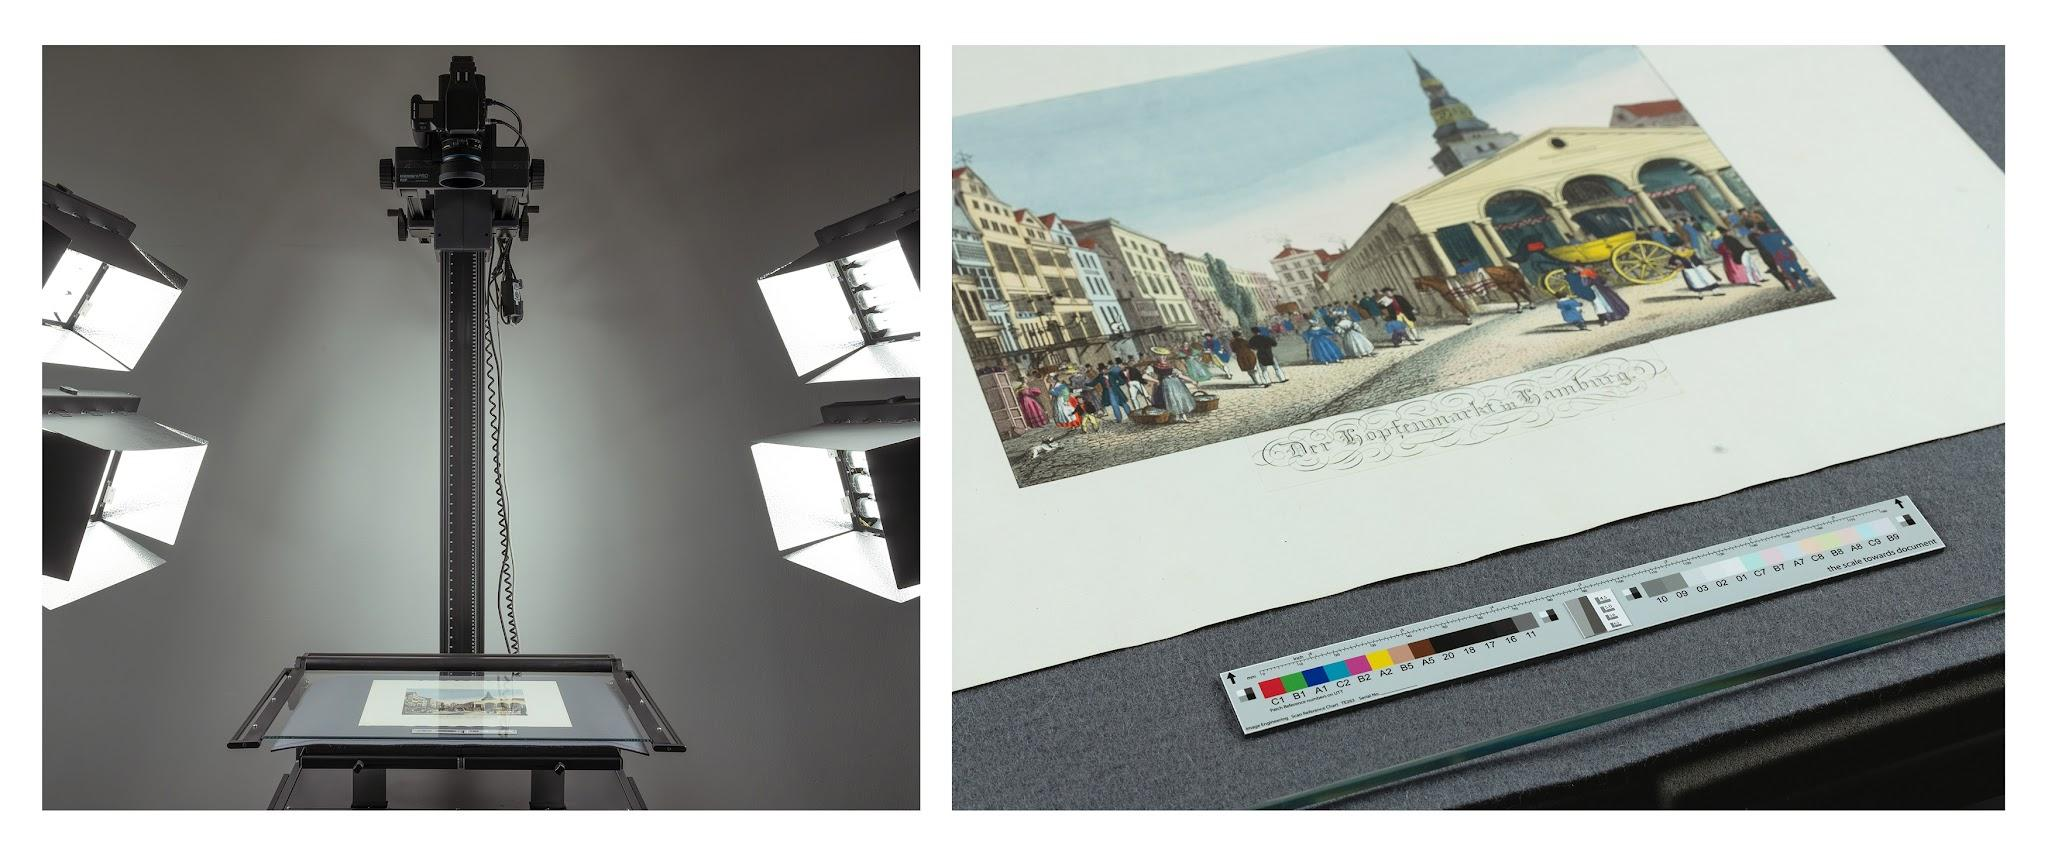
\includegraphics{media/buchscanner.jpg}

}

\caption{\label{fig-buchscanner}Beispiel eines Auflichtscanners}

\end{figure}%

Die 2D-Scanner können sich in verschiedenen Eigenschaften wie Größe der
Formate, Farbtiefe, Auflösung, Art und Qualität der Optik und Mechanik
sowie in der Verarbeitungsgeschwindigkeit unterscheiden. Um eine hohe
und gleichbleibende Bildqualität zu gewährleisten, ist eine regelmäßige
Kalibrierung der Systeme und Auswertung der Aufnahmen anhand von
Test-Targets (z.\,B.~UTT-Target oder GoldenThread) erforderlich. Neben
der Hardware unterscheiden sich Scanner in der Software, durch die
Rohdaten des Scanners für die weitere Nutzung bearbeitet
(z.\,B.~beschnitten oder geglättet), optimiert und in gewünschten
Zielformaten gespeichert werden.

\subsubsection{3D}\label{d-1}

Bei der 3D-Erfassung eines Objektes kann zwischen foto- und
scanbasierten Verfahren unterschieden werden.

So werden bei der Photogrammetrie Fotos aus verschiedenen Blickwinkeln
aufgenommen. Dabei wird die Anzahl der Fotos derart erhöht, dass sie mit
Hilfe von Software zu einem 3D-Modell verarbeitet werden können. Nach
diesem Prinzip funktionieren auch 3D-Scanning-Apps für Smartphones, die
3D-Scans von Objekten mithilfe der Kamera eines Smartphones ermöglichen.

Demgegenüber stehen verschiedene Scanverfahren. Beim Laserscanning
werden z.\,B.~Laserstrahlen auf das Objekt gerichtet, und die
reflektierten Daten werden verwendet, um ein präzises 3D-Modell zu
erstellen. Neben dem Laser lassen sich solche 3D-Modelle auch mit
strukturiertem Licht (Streifenlichtscans) oder Computertomographie
erzeugen.

Bei der 3D-Modellierung wird ein 3D-Modell nach Vorlagen manuell und mit
Hilfe von spezifischer Software erstellt. Dies kommt insbesondere für
die digitale Rekonstruktion von physisch nicht erhaltenen (Teilen von)
Objekten zur Anwendung.

Alle Verfahren können miteinander kombiniert werden.

Wird beispielsweise ein Pop-up Buch oder ein Globus 3D-digitalisiert,
sollen zusätzlich die kinetischen Aspekte (ein Globus dreht sich um
seine Achse, bei einem Pop-up Buch lässt sich eine Lasche herausziehen
usw.) unter Umständen auch im Digitalisat nachvollziehbar bleiben.
Besteht das Originalobjekt aus Einzelteilen und werden diese
entsprechend in Segmenten digitalisiert, können diese Segmente
interaktiv nutzbar gemacht werden und/oder Animationen eingesetzt
werden. Ein einfacher Scan reicht in diesem Fall nicht aus, da hier
lediglich „die Hülle im Ganzen`` erfasst wird. Eine manuelle
Nachbearbeitung ist nötig.

\subsection{Workflowmanagementsysteme}\label{workflowmanagementsysteme}

Bei diesen Systemen handelt es sich im Grunde um klassische
Workflowmanagementsysteme
(\href{https://de.wikipedia.org/wiki/Workflow-Management-System}{WMS}),
die auf die Abbildung und Modellierung der \hyperref[prozesse]{oben
beschriebenen Prozesse} spezialisiert sind. Das Ziel der Systeme ist es,
die Prozesse technisch abzubilden und zu organisieren bzw.~die Zustände
der im Prozess befindlichen Objekte zu speichern und darzustellen.

\begin{figure}

\centering{


\includegraphics{index_files/mediabag/media/wms_workflow.pdf}

}

\caption{\label{fig-wms-workflow}Beispiel für einen im WMS
eingerichteten Workflow}

\end{figure}%

Aufgrund der hohen Spezialisierung ist die Auswahl an WMS für
bibliothekarische Digitalisierungsprozesse überschaubar. Dazu gehören
sowohl kommerzielle Produkte, wie
z.\,B.~\href{https://www.semantics.de/visual_library/}{Visual Library}
aber auch frei verfügbare Open-Source-Systeme wie
\href{https://www.kitodo.org/}{\emph{Kitodo}}.

Der wesentliche Unterschied zwischen den Tools~-- neben der Frage der
Lizenz~-- ist deren Modularität. Bei einigen Lösungen sind z.\,B.~die
Erstellung, Anreicherung und Präsentation fest in einem System
zusammengefasst, andere wählen z.\,B.~den Ansatz, die Präsentation von
der Erstellung zu trennen, sodass die Darstellung z.\,B.~auch mit
spezialisierten Präsentationswerkzeugen, wie Content-Management-Systemen
erfolgen kann.

\subsection{Metadaten und
Schnittstellen}\label{metadaten-und-schnittstellen}

An vielen Stellen des Digitalisierungsprozesses sind Schnittstellen
(APIs) zu Drittsystemen notwendig. Das gilt sowohl für die Einbindung
externer Metadaten (beispielsweise der Import aus Nachweissystemen via
{SRU} aus Verbundkatalogen oder Kalliope) als auch die Weitergabe von
Daten an externe Portale wie die Deutsche Digitale Bibliothek
(\emph{DDB}).

Als Austauschformat verwenden diese Schnittstellen meist
\hyperref[xml-basierte-datenformate]{XML-Datenformate} wie
\emph{PICA/XML}, \emph{METS/MODS}, \emph{EAD} und \emph{LIDO}, die auf
Struktur- oder Metadaten digitalisierter Objekte spezialisiert sind.
\hyperref[schnittstellen]{Relevante Schnittstellen} sind vor allem
{SRU}, {OAI-PMH} und {IIIF}. Die Nutzung gemeinsamer Datenformate
ermöglicht unter anderem die Auffindbarkeit, Verknüpfung, Präsentation
und Verwendung von Objekten in unterschiedlichen Zusammenhängen.

Für einzelne Ressourcentypen und Anwendungen existieren oft genauere
Anwendungsprofile, die die Verwendung von Metadatenstandards erweitern
oder einschränken.

\textbf{Beispiel:} Das
METS/MODS-\href{https://wiki.deutsche-digitale-bibliothek.de/display/DFD/5.+Anwendungsprofile+und+Best+Practice+Guides}{Anwendungsprofile}
der Deutschen Digitalen Bibliothek legt Anforderungen an Metadaten fest,
wenn diese in das Portal eingebunden werden sollen. Zur
\href{https://wiki.deutsche-digitale-bibliothek.de/display/DFD/Schematron-Validierungen+der+Fachstelle+Bibliothek\#SchematronValidierungenderFachstelleBibliothek-Schematron-Dateien}{Validierung
der Daten} stellt die DDB passende Werkzeuge zur Verfügung.

\subsection{Betriebsmodelle}\label{betriebsmodelle-1}

Bei dem Einsatz der Werkzeuge im Digitalisierungsprozess stellt sich
immer die Frage, ob sich die Anschaffung der Hardware oder die
hausinterne Installation und Anpassung von Software lohnt oder aber
Bestandteile ausgelagert werden können. Wie bei allen IT-Systemen sind
grundsätzlich \hyperref[sec-betriebsmodelle]{drei Betriebsmodelle}
denkbar:

\begin{itemize}
\item
  \textbf{Lokale Installation}: Hard- und Software wird durch
  betriebseigenes Personal gehostet, betreut und weiterentwickelt.
  Dieses Modell ist vor allem dann empfehlenswert, wenn bereits
  Digitalisierungskompetenz in der Institution vorhanden ist und die
  Digitalisierung einen dauerhaften Schwerpunkt in den Alltagsprozessen
  einnimmt bzw.~einnehmen soll.
\item
  \textbf{Externes (Cloud-)Hosting}: Sofern nicht z.\,B.~rechtliche
  Gründe dagegen sprechen, ist dieses Modell empfehlenswert, wenn nur
  punktuell oder in geringem Umfang digitalisiert werden soll und dabei
  keine eigene Expertise notwendig ist oder aufgebaut werden soll.
\item
  \textbf{Hybridlösungen:} Es werden nur Teile des Prozesses
  ausgelagert, z.\,B.~das Scannen der Objekte, während z.\,B.~die
  Inhaltsanreicherung durch Metadaten im Haus verbleibt.
\end{itemize}

Die Hybridvariante wird im Alltag am häufigsten umgesetzt. Die
Herausforderung besteht darin, die Schnittstellen zwischen externen und
internen Prozessen genau zu definieren und festzulegen. So muss zum
Beispiel externen Scandienstleistern Zugriff auf das intern betreute
Workflowmanagementsystem gewährt werden, damit digitalisierte Objekte
direkt im System abgelegt werden können.

\section{Digitalisierung als Beitrag zur Open
GLAM-Bewegung}\label{digitalisierung-als-beitrag-zur-open-glam-bewegung}

Mit der Digitalisierung leisten Bibliotheken und andere
GLAM-Einrichtungen wichtige Beiträge dazu, dass Kulturgüter weltweit
zugänglich, gut auffindbar und nachnutzbar sind. Neben der
einrichtungseigenen Präsentation und aggregierenden Portalen wie der
„Deutschen Digitalen Bibliothek`` oder der „Europeana`` spielen auch
offene Wissensplattformen im Web eine wichtige Rolle, um Daten
zugänglich zu machen, zu teilen und Nutzende an der Erschließung zu
beteiligen. Entsprechende Möglichkeiten sollen im Folgenden skizziert
werden, da es sich um einen wichtigen Trend bei der Digitalisierung und
Nutzung handelt.

Offener Zugang und offene Lizenzen für freie Nutzungsszenarien,
standardisierte Schnittstellen und offene Metadaten vereinfachen das
Teilen von Daten bzw.~Informationen aus digitalisierten Quellen --
Texten, Illustrationen und Sammlungen~-- als freies Wissen.

\subsection{Veranstaltungsformate und
Handlungsfelder}\label{veranstaltungsformate-und-handlungsfelder}

Hackathons und Editathons sind Veranstaltungsformate, um kurzfristig die
Bekanntheit digitaler Sammlungen zu steigern, Datenexperimente zu
ermöglichen und Datenkollaborationen in Pilotprojekten anzustoßen und
dabei können Impulse für weiterentwickelte Datenanwendungen entstehen.
Lerneffekte entstehen dabei nicht nur bei den beteiligten Menschen,
sondern auch institutionell bei den beteiligten Bibliotheken und anderen
GLAM, die ggf.~Bedürfnisse, Ideen und Defizite von Nutzenden
kennenlernen. Ein Beispiel Hackathons ist die Initiative
\href{https://codingdavinci.de/}{„Coding da Vinci``}.

Crowdsourcing und Citizen Science sind Handlungsfelder, die in
Bibliotheken zunehmend Aufmerksamkeit wecken. Hierbei gewinnen
Bibliotheken über externe engagierte Dritte zusätzliche Ressourcen für
die Erschließung, Auswertung oder Korrektur von Daten.

\begin{tcolorbox}[enhanced jigsaw, leftrule=.75mm, toprule=.15mm, left=2mm, opacityback=0, arc=.35mm, colback=white, breakable, colframe=quarto-callout-tip-color-frame, rightrule=.15mm, bottomrule=.15mm]
\begin{minipage}[t]{5.5mm}
\textcolor{quarto-callout-tip-color}{\faLightbulb}
\end{minipage}%
\begin{minipage}[t]{\textwidth - 5.5mm}

\vspace{-3mm}\textbf{Beispiel}\vspace{3mm}

Im Projekt „\href{https://de.wikiversity.org/wiki/DieDatenlaube}{Die
Datenlaube}`` erfasst und korrigiert in der deutschsprachigen Wikisource
eine Gemeinschaft Ehrenamtlicher seit 2008 die von verschiedenen
Bibliotheken bereitgestellten Scans der Illustrierten „Die
Gartenlaube``. Diese Wikisource-Volltexte und -Illustrationen werden mit
offenen Metadaten in Wikidata strukturiert erschlossen.

\begin{figure}[H]

\centering{

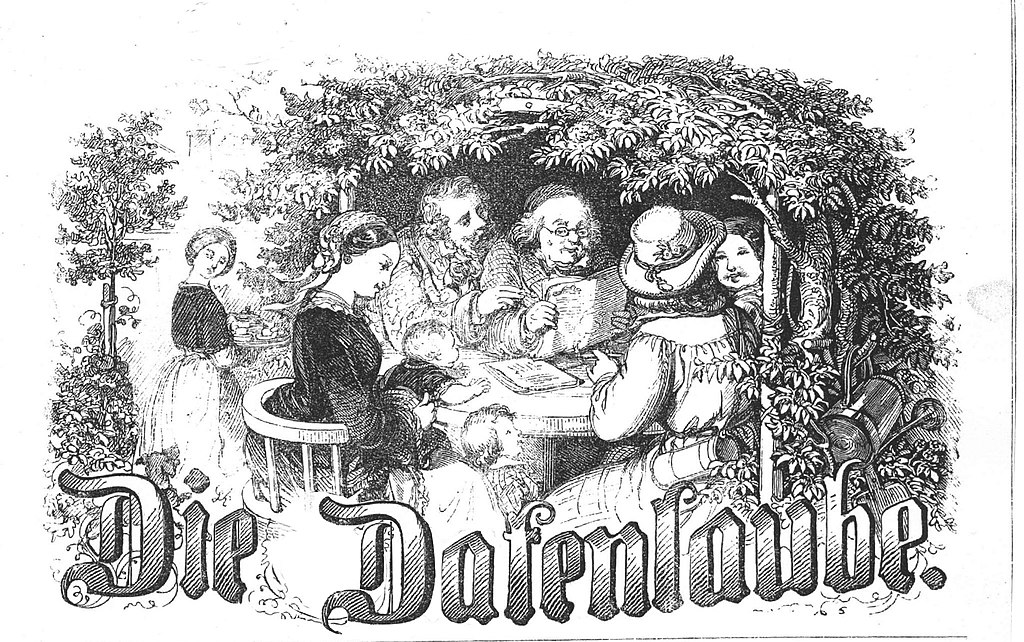
\includegraphics[width=0.45\textwidth,height=\textheight]{media/die-datenlaube.jpg}

}

\caption{\label{fig-datenlaube}Die Datenlaube: Projektlogo}

\end{figure}%

\end{minipage}%
\end{tcolorbox}

\subsection{Offene Infrastrukturen}\label{offene-infrastrukturen}

Offene digitale Infrastrukturen spielen für die Speicherung,
Erschließung und Vernetzung von Digitalisaten eine wichtige Rolle, nicht
zuletzt auch, um die beschriebene Beteiligung zu ermöglichen. Das
prominenteste Beispiel dafür sind die Projekte der Wikimedia-Foundation,
deren Grundprinzipien von Offenheit und Referenzierbarkeit die
bibliothekarischen Erschließungs- und Präsentationskomponenten ergänzen:

\begin{itemize}
\item
  \textbf{Wikimedia Commons} fungiert als zentraler Medienspeicher. Die
  Erschließung kann bis zu Details von Bildpositionen reichen. Die
  Illustrationen dieses Handbuchs sind in Wikimedia Commons
  \href{https://commons.wikimedia.org/wiki/Category:Handbuch_IT_in_Bibliotheken}{in
  einer Medienkategorie} gebündelt (siehe Abbildungsverzeichnis im
  Anhang~\ref{sec-abbildungen}).
\item
  Mit der offenen Wissensdatenbank (Knowledge Graph) \textbf{Wikidata}
  können insbesondere Metadaten strukturiert und damit maschinenlesbar
  gespeichert, gemeinsam editiert, visualisiert, analysiert, geteilt und
  verknüpft werden.
\item
  Die vielsprachigen Versionen der \textbf{Wikipedia} speichern Wissen
  in enzyklopädischen Artikeln und ermöglichen so die Zusammenführung
  von Digitalisaten mit Texten, Illustrationen aus den Wikimedia
  Commons, Referenzen, Links und damit Kontext.
\item
  \textbf{Wikisource} ist eine Quellensammlung gemeinfreier Werke und
  besteht sowohl aus transkribierten Volltexten und deren Illustrationen
  als auch thematischen Linksammlungen zu relevanten Digitalisaten in
  digitalen Sammlungen öffentlicher und wissenschaftlicher Bibliotheken,
  Archive, Museen und Galerien (GLAM).
\end{itemize}

Herausforderungen aus IT-bibliothekarischer Sicht bestehen darin,
Wikimedia-Portale und bibliothekarische Werkzeuge durch Schnittstellen
und Datentransformation (\hyperref[etl-prozess]{ETL-Tools}) miteinander
zu verknüpfen. GLAM-Labore (Open GLAM Labs) können dafür als
Experimentier- und Ausbildungsort fungieren~-- in Bibliotheken und
institutionenübergreifend z.\,B.~im Rahmen von
Landesdigitalisierungsprogrammen.

\section{Checkliste für
Digitalisierungsprojekte}\label{checkliste-fuxfcr-digitalisierungsprojekte}

Diese \textbf{Checkliste} dient als Leitfaden für die Planung und
Umsetzung von Digitalisierungsprojekten in Bibliotheken und hilft
sicherzustellen, dass die Ziele erreicht und die digitalen Sammlungen
effektiv genutzt werden können.

\textbf{Vorbereitungsphase:}

\begin{enumerate}
\def\labelenumi{\arabic{enumi}.}
\item
  \emph{Festlegung der Ziele}: Klären Sie die Hauptziele und den Zweck
  der Digitalisierung (z.\,B.~Zugänglichkeit, Erhaltung, Forschung).
\item
  \emph{Ressourcenplanung}: Ermitteln Sie die erforderlichen Ressourcen
  wie Verfügbarkeit der Objekte, Personal, Technologie, Budget und
  Zeitrahmen.
\item
  \emph{Rechtliche Überlegungen}: Klären Sie urheberrechtliche und
  rechtliche Fragen bezüglich der digitalisierten Materialien.
\item
  \emph{Auswahl der Objekte}: Wählen Sie die Objekte aus, die
  digitalisiert werden sollen, u.\,a.~basierend auf ihrer Bedeutung und
  ihrem Zustand.
\item
  \emph{Metadatenplanung}: Entwickeln Sie einen Plan zur Erfassung und
  Verwaltung von Metadaten für die digitalisierten Materialien.
\end{enumerate}

\textbf{Technische Umsetzung:}

\begin{enumerate}
\def\labelenumi{\arabic{enumi}.}
\setcounter{enumi}{5}
\item
  \emph{Scantechnologie}: Wählen Sie die geeignete Scantechnologie und
  Auflösung entsprechend der Art der Objekte und deren Verwendungszweck
  aus.
\item
  \emph{Qualitätskontrolle}: Implementieren Sie Prozesse zur
  Sicherstellung der Qualität der Digitalisate.
\item
  \emph{Dateiformate}: Entscheiden Sie über die geeigneten Dateiformate
  für die digitalisierten Materialien.
\item
  \emph{Speicher und Sicherung}: Planen Sie die Speicherung und
  regelmäßige Sicherung der digitalen Sammlung.
\end{enumerate}

\textbf{Metadaten und Beschreibung:}

\begin{enumerate}
\def\labelenumi{\arabic{enumi}.}
\setcounter{enumi}{9}
\item
  \emph{Metadatenstandards}: Verwenden Sie etablierte
  Metadatenstandards, um die Beschreibung der Objekte zu
  standardisieren.
\item
  \emph{Dokumentation}: Dokumentieren Sie den Digitalisierungsprozess
  und die verwendeten Metadaten.
\item
  \emph{Zugänglichkeitsprüfung}: Überprüfen Sie, ob die digitalen
  Sammlungen barrierefrei und benutzerfreundlich sind.
\end{enumerate}

\textbf{Langzeitpflege}:

\begin{enumerate}
\def\labelenumi{\arabic{enumi}.}
\setcounter{enumi}{12}
\item
  \emph{Erhaltungsstrategien}: Planen Sie langfristige
  Erhaltungsstrategien für digitale Materialien.
\item
  \emph{Aktualisierung und Migration}: Berücksichtigen Sie die
  Notwendigkeit von Aktualisierungen und Migrationen von Dateiformaten
  und Systemen.
\end{enumerate}

\textbf{Zugang und Bereitstellung:}

\begin{enumerate}
\def\labelenumi{\arabic{enumi}.}
\setcounter{enumi}{14}
\item
  \emph{Plattformwahl}: Wählen Sie die geeignete Plattform oder das
  geeignete System zur Präsentation und Verwaltung der digitalen
  Sammlungen.
\item
  \emph{Nutzungsrechte}: Klären Sie die Nutzungsrechte und -bedingungen
  für die digitalen Inhalte.
\item
  \emph{Nutzerfeedback}: Implementieren Sie Mechanismen zur Erfassung
  von Nutzerfeedback zur Verbesserung der digitalen Sammlungen.
\end{enumerate}

\textbf{Veröffentlichung und Dissemination:}

\begin{enumerate}
\def\labelenumi{\arabic{enumi}.}
\setcounter{enumi}{17}
\item
  \emph{Verbreitung}: Planen Sie die Verbreitung der digitalisierten
  Sammlungen über Onlinekanäle, soziale Medien und Partnerschaften.
\item
  \emph{Marketing}: Entwickeln Sie Marketingstrategien, um die digitalen
  Sammlungen einem breiten Publikum bekannt zu machen.
\item
  \emph{Evaluation}: Führen Sie regelmäßige Bewertungen durch, um den
  Erfolg Ihrer Digitalisierungsprojekte zu messen und zu verbessern.
\end{enumerate}

\section{Zusammenfassung und
Ausblick}\label{zusammenfassung-und-ausblick-4}

Viele Bibliotheken mit historischen Beständen sind im Feld der
Kulturgutdigitalisierung engagiert und kooperativ unterwegs. Werkzeuge,
Standards und Dienstleister stehen zur Verfügung, um die unikalen
Bestände ins Netz zu bringen. Um die Bandbreite der Objekte zu
erweitern, finden gerade wichtige Entwicklungen statt, um auch AV-Medien
und Objekte jenseits von 2D in die Routine aufzunehmen. Ebenso werden
die Bibliotheken mit den Ergebnissen aus OCR-D immer mehr in der Lage
sein, auch ohne Expertenwissen gute Volltexte zu erzeugen bzw.~ihre
gesamten Digitalisate inkl.~handschriftlicher Dokumente mit Volltexten
anzureichern. Hier sind ggf.~auch kooperative Infrastrukturen
aufzubauen, um die Fortschritte in den technischen Möglichkeiten schnell
zur Verfügung zu stellen und eine regelmäßige Erneuerung der Volltexte
zum Standard werden zu lassen. Daneben gilt es, gezielt
\hyperref[kompetenzen]{Kompetenzaufbau} unter den Mitarbeitenden zu
betreiben, um den Aufbau und Betrieb solcher Infrastrukturen zu
gewährleisten.

Erste Bibliotheken machen sich mit der schnell wachsenden Menge an
Volltexten auf den Weg, mit Hilfe ausgewählter Tools aus dem Feld des
Maschinenlernens, ihre Suche semantisch anzureichern auf Basis der
vorgeschalteten automatisierten Analyseverfahren.

Mit dem großen Schatz der Volltexte wird es darüber hinaus wichtiger
werden, diesen auch den Forscher*innen zusätzlich über eine API
anzubieten, um individuelle Korpora für den Download in eigene
Umgebungen zusammenstellen zu können. Bislang gibt es jedoch noch keine
umfassende und nachhaltige Lösung, die sowohl flexible
Forschungsmöglichkeiten als auch den Schutz von Urheberrechten
vollständig gewährleistet.

Aber auch die kollaborativen Aktivitäten an einzelnen Digitalisaten im
Wikiversum oder in Citizen Science Projekten sind getragen von dem
Leitgedanken, dass die digitalisierten Kulturgüter in neue Zusammenhänge
gestellt werden und Interessierte zu einem Thema zusammenbringen.

\bookmarksetup{startatroot}

\chapter{Forschungsnahe Dienste}\label{sec-forschungsnahe-dienste}

\begin{tcolorbox}[enhanced jigsaw, leftrule=.75mm, toprule=.15mm, left=2mm, opacityback=0, arc=.35mm, colback=white, breakable, colframe=quarto-callout-note-color-frame, rightrule=.15mm, bottomrule=.15mm]
\begin{minipage}[t]{5.5mm}
\textcolor{quarto-callout-note-color}{\faInfo}
\end{minipage}%
\begin{minipage}[t]{\textwidth - 5.5mm}

\vspace{-3mm}\textbf{Zusammenfassung}\vspace{3mm}

Bibliotheken bieten \hyperref[einleitung]{Dienste für die Wissenschaft}
im Rahmen des digitalen Wandels von Publikationsprozessen und Open
Science an. Dazu gehören in diesem Kapitel vorgestellte
\hyperref[publikationsdienste]{Dienste zur Publikation}, zur
\hyperref[forschungsdatenmanagement]{Verwaltung von Forschungsdaten} und
\hyperref[forschungssoftware]{Forschungssoftware} sowie
\hyperref[forschungsinformationssysteme]{Informationen über
Forschungsprozesse}. Abschließend werden verschiedene übergreifende
Themen wie \hyperref[zertifikate-und-standards]{Zertifikate und
Standards} und \hyperref[langzeitarchivierung]{Langzeitarchivierung}
behandelt.

\end{minipage}%
\end{tcolorbox}

\section{Einleitung}\label{einleitung-8}

Unter forschungsnahen Diensten werden verschiedene Bibliotheksservices
zusammengefasst, die Wissenschaftler*innen im gesamten Forschungsprozess
unterstützen und die überwiegend im Kontext von digitalem Wandel und
Open Science angesiedelt sind
(\url{https://www.o-bib.de/bib/article/view/5718}). Dazu zählen
z.\,B.~Services in den Bereichen
\hyperref[forschungsdatenmanagement]{Forschungsdatenmanagement},
Bibliometrie sowie verschiedene
\hyperref[publikationsdienste]{Publikationsdienste}.

Einige dieser Dienste, z.\,B. Repositorien für Zeitschriftenartikel, die
unter Open-Access-Bedingungen zweitveröffentlicht werden dürfen, gehören
schon seit Jahrzehnten zum Dienstleistungsrepertoire wissenschaftlicher
Bibliotheken. Inzwischen betreiben größere Einrichtungen zudem oft
spezialisierte Repositorien für ein Spektrum verschiedener Objekttypen:
Publikationen wie Zeitschriften, Monografien und Sammelbände, sowie Open
Educational Resources ({OER}), Forschungsdaten, Forschungssoftware und
mehr. Dazu gehören auch diverse Dienste, die übergreifend den
Forschungsoutput bestimmter lokaler oder fachlicher
Forschungscommunities besser auffindbar oder messbar machen sollen.
Darunter fallen Forschungsinformationssysteme und Dienstleistungen im
Bereich von Metriken oder zur Verwaltung von
Artikelveröffentlichungsgebühren in Open-Access-Journals (\emph{APCs}).

\begin{tcolorbox}[enhanced jigsaw, leftrule=.75mm, toprule=.15mm, left=2mm, opacityback=0, arc=.35mm, colback=white, breakable, colframe=quarto-callout-important-color-frame, rightrule=.15mm, bottomrule=.15mm]
\begin{minipage}[t]{5.5mm}
\textcolor{quarto-callout-important-color}{\faExclamation}
\end{minipage}%
\begin{minipage}[t]{\textwidth - 5.5mm}

\textbf{Open Science} bezeichnet den Ansatz, wissenschaftliche
Forschungsergebnisse, Daten und Methoden frei zugänglich und transparent
zu teilen. Teilaspekte davon sind Open Access, Open Data, OER und Open
Source. Ziel ist es, die Zusammenarbeit sowie die Reproduzierbarkeit von
Forschung zu fördern, Innovationen zu beschleunigen und den
gesellschaftlichen Nutzen wissenschaftlicher Erkenntnisse zu maximieren.
Dieser offene Ansatz erleichtert es Forschenden weltweit, Informationen
frei zu nutzen, zu teilen und weiterzuentwickeln.

\end{minipage}%
\end{tcolorbox}

Forschungsförderer und Ministerien erwarten in Deutschland mittlerweile
von den Forschungseinrichtungen eine Transformation des
Publikationswesens hin zu Open Access und Open Data. Dazu gehören
themenbezogene institutionelle Policies, Beratungs- und
Schulungsangebote sowie technische Dienste. Auf der Ebene der
europäischen Forschungsförderung wird u.\,a.~versucht, durch Initiativen
wie \emph{\href{https://coara.eu/}{CoARA}} die Maßstäbe der
Forschungsbewertung weiterzuentwickeln - weg von klassisch
bibliometrischen Indikatoren wie h-Index und Journal-Impact-Factor hin
zu einer Würdigung vielfältiger Forschungsergebnisse.

In Abgrenzung zur Dominanz von Großverlagen ist im Bereich der
wissenschaftlichen Informationsinfrastrukturen darüber hinaus der
Anspruch entstanden, Dienste~-- bis hin zur Ebene von Entwicklung und
Betrieb zugehöriger IT-Infrastrukturen~-- durch die Communities der
Forschenden selbst zu betreiben. In der englischsprachigen
Fachdiskussion sind dazu Begriffe wie „scholar-led publishing`` oder
„scholar-led conferences`` geprägt worden, vgl.~exemplarisch hierzu das
\emph{\href{https://graphite.page/scholar-led-manifesto/}{Scholar-Led.Network
Manifesto}}. Bibliotheken sehen sich hier als vertrauenswürdige,
öffentlich finanzierte Dienstleister für die Wissenschaftscommunities.

Der Einsatz von und die aktive Mitarbeit an Open-Source-Software ist bei
den forschungsnahen Diensten stärker als in anderen Bereichen der
Bibliotheks-IT eine Selbstverständlichkeit. Auch die Bedeutung der
gemeinschaftlichen Pflege offener Standards, Datenmodelle und
Daten-Gemeingüter ist hier besonders ausgeprägt.

\section{Publikationsdienste}\label{publikationsdienste}

Die Veröffentlichung wissenschaftlicher Erkenntnisse ist ein zentraler
Bestandteil des wissenschaftlichen Arbeitens. Solange sich dieser
Prozess noch in den Geschäftsprozessen klassischer
Subskriptionszeitschriften abbildete, befanden sich wissenschaftliche
Bibliotheken eher auf der Seite der Medienbereitstellung. Mit
zunehmender Stärkung des Open-Access-Gedankens und dem Aufkommen neuer
Geschäftsmodelle rückten wissenschaftliche Bibliotheken stärker in die
Rolle des*der Unterstützenden und Ermöglichenden. Die Digitalität der
gesamten Prozesskette vom Schreiben bis zur Veröffentlichung der
Beiträge in teilweise von den Bibliotheken getragenen Infrastrukturen
erfordert die Einbindung unterschiedlicher IT-Werkzeuge, die im
Folgenden näher beschrieben werden.

\subsection{Dienste für Journals und andere
Publikationsformen}\label{dienste-fuxfcr-journals-und-andere-publikationsformen}

Open Access bedeutet, dass wissenschaftliche Literatur kostenfrei und
öffentlich im Internet zugänglich ist, sodass Interessierte die
Volltexte lesen, herunterladen, kopieren, verteilen, drucken, in ihnen
suchen, auf sie verweisen und sie auch sonst auf jede denkbare legale
Weise benutzen können, ohne finanzielle, gesetzliche oder technische
Barrieren jenseits von denen, die mit dem Internetzugang selbst
verbunden sind. Zum ersten Mal wurde dieser Gedanke in der
\emph{\href{https://www.budapestopenaccessinitiative.org/}{Grundsatzerklärung
der Budapester Open-Access-Bewegung}} formuliert.

Durch die Transformationsprozesse im wissenschaftlichen
Publikationswesen weg von den traditionellen Abonnementmodellen hin zu
Open Access sehen sich Bibliotheken zunehmend auch in der Rolle von
Publikationsdienstleistern. Dies kann einerseits die Gründung eines
Universitätsverlages bedeuten, andererseits aber auch die Bereitstellung
der notwendigen Infrastruktur für wissenschaftliche Zeitschriften.
Begünstigt durch Kostenverschiebung vom Lesen hin zum Publizieren wird
der scholar-led-Ansatz immer gefragter und Bibliotheken müssen in diesem
Bereich Expertise aufbauen.

Zur Schaffung einer technischen Infrastruktur für Zeitschriften lässt
sich z.\,B. mit der Software
\emph{\href{https://ojs-de.net/ueber-ojs}{Open Journal Systems (OJS)}}
eine Plattform zur Verfügung stellen, welche die strukturierte
Veröffentlichung von Zeitschriften(-artikeln) ermöglicht. Parallel dazu
müssen auch die erforderlichen Abläufe und Organisationsstrukturen
angepasst werden. Personelle Ressourcen müssen hier ebenso bedacht
werden. In erster Linie gilt es, die Herausgeber*innen-Teams der
Zeitschriften zu unterstützen. Gleichzeitig sollte die Bibliothek auch
technischen Support für einreichende Autor*innen bieten. Der
Funktionsumfang von {OJS} ermöglicht es auch, einen Workflow für den
Peer-Review-Prozess abzubilden. Auch hier liegt Potenzial für die
Unterstützung durch Bibliotheken. Wichtig ist somit ein Überblick über
den Gesamtprozess des wissenschaftlichen Publizierens und nicht nur die
Softwareaspekte. Für die Publikation von Monographien gibt es z.\,B.~mit
\href{https://pkp.sfu.ca/software/omp/}{Open Monograph Press} ({OMP})
eine Software, die von der gleichen Organisation wie {OJS} angeboten und
weiterentwickelt wird.

Parallel dazu entwickeln sich derzeit alternative
Publikations-Plattformen wie Preprint-Dienste, (Micro-)Blogs, Data
Journals und ähnliche Dienste, die traditionelle Publikationswege wie
peer-reviewte Journals ergänzen, siehe dazu auch die entsprechende
\href{https://doi.org/10.21428/996e2e37.3ebdc864}{Publikation der
Initiative Knowledge Exchange}. Hier können Bibliotheken ebenso in die
Rolle der Dienstleistenden treten, Instanzen geeigneter
Open-Source-Software hosten und diese Entwicklung unterstützen. Dies
kann auch im Zusammenhang mit der externen Kommunikation von
Bibliotheken (Kapitel~\ref{sec-kommunikation}) betrachtet werden.
Ergänzend gibt es zahlreiche weitere Dienste, die das
Open-Access-Publizieren vor allem administrativ unterstützen, von denen
im Folgenden einige kurz erläutert werden.

\subsection{Open-Access-Dienste}\label{open-access-dienste}

Neben der Unterstützung bei Open-Access-Veröffentlichungen haben sich im
Zusammenhang mit der Open-Access-Transformation weitere IT-Dienste in
Bibliotheken entwickelt.

\subsubsection{Verlags-Software}\label{verlags-software}

Da im Sinne der „scholar-led infrastructure`` zunehmend
Universitätsverlage gegründet werden, existieren hier auch eigene
Softwarelösungen für die Verwaltung der Titel, Lagerbestände,
Kund*innen-, Adress- und Versanddaten. Häufig ist ein eigener Webshop
mit entsprechenden Funktionalitäten integriert und es gibt
Schnittstellen zur Buchhaltung und Auslieferung. Für kleinere Verlage
reicht vermutlich ein einfacher Webshop aus; Spezialsoftware kann
verlagsspezifische Anforderungen allerdings besser abbilden. Betrieb und
Administration der Programme gehören mit in das zugehörige
Dienstleistungsportfolio.

\subsubsection{Publikationsfonds-Verwaltung}\label{publikationsfonds-verwaltung}

Publikationsfonds zur Finanzierung von Open-Access-Publikationen sind an
vielen wissenschaftlichen Bibliotheken fest verankerte Hilfsmittel, um
die Transformation des wissenschaftlichen Publikationswesens hin zu Open
Access zu unterstützen. Durch sie werden anfallende \emph{Article
Processing Charges} ({APC}) entsprechend vorgegebener Kriterien der
Einrichtung (mindestens anteilig) zentral gezahlt. Zum Monitoring der
entstehenden Kosten ist häufig eine Tabellenkalkulationssoftware
ausreichend. Für einen Vergleich verschiedener Einrichtungen und ein
einheitliches Reporting existieren jedoch Services wie
\emph{\href{https://openapc.net/}{OpenAPC}}. Zur einheitlichen
Darstellung aller Publikationskosten hat sich mit
\emph{\href{https://www.opencost.de/metadatenschema/}{OpenCost}} ein
XML-Metadatenschema etabliert.

\subsubsection{Open Refine}\label{open-refine}

Sollen Daten aus unterschiedlichen Quellen zusammengeführt werden oder
ein Abgleich gegen externe Datenbanken stattfinden, ist
\emph{\href{https://openrefine.org/}{OpenRefine}} ein geeignetes
Werkzeug: Über offene Schnittstellen können Datensätze sowohl erweitert
als auch beispielsweise in Wikidata exportiert werden. Hierbei ist keine
zentrale Installation notwendig. Die Software wird lokal auf den
Endgeräten ausgeführt. Lediglich eine korrekte Einstellung der Firewall,
um die Kommunikation mit externen Datenbanken zu ermöglichen, gilt es zu
beachten.

\subsubsection{Journal-Finder-Werkzeuge}\label{journal-finder-werkzeuge}

Neben den üblichen Fragen zu Lizenzen bei Open-Access-Publikationen
spielt auch die Wahl eines geeigneten Journals eine zentrale Rolle.
Derzeit verbreitete Journal-Finder-Werkzeuge wie
\emph{\href{https://service.tib.eu/bison/}{B!SON}} oder der
\emph{\href{https://finder.open-access.network/}{oa.finder}} greifen für
die Journal-Daten zwar beide auf das \emph{Directory of Open Access
Journals} (\emph{\href{https://doaj.org/}{DOAJ}}) zu, verfolgen jedoch
unterschiedliche Ansätze. Der \emph{oa.finder} zeigt eine Liste von
Zeitschriften mit Filteroptionen und den jeweiligen Förderbedingungen
an. Diese werden aus bestehenden Transformationsverträgen abgeleitet und
enthalten keine spezifischen Förderbedingungen. \emph{B!SON} bietet
teilnehmenden Einrichtungen die Möglichkeit, eine eigene Liste mit
Förderbedingungen zu hinterlegen. Treffer werden direkt mit den
korrekten Förderbedingungen angezeigt. Zu diesem Zweck muss ein
Web-Backend entsprechend der Vertragssituation gepflegt werden.

\subsection{Repositorien für
Forschungsergebnisse}\label{repositorien-fuxfcr-forschungsergebnisse}

Zentral für die Veröffentlichung jedweder Art von wissenschaftlichem
Output ist ein geeigneter Ort für deren Veröffentlichung, ganz besonders
im Hinblick auf die zunehmende Datengetriebenheit der Wissenschaften.

Heute haben sich Open-Access-Repositorien als verlässliche
Speicherdienste für wissenschaftliche Ergebnisse etabliert, seien es
Forschungsdaten, textuelle Publikationen oder andere Materialien. Für
die wissenschaftliche Kommunikation ist dabei die Zitierbarkeit eine
wichtige Voraussetzung. Dazu muss sichergestellt werden, dass
publizierte Ergebnisse in der veröffentlichten Form erhalten werden, das
heißt nicht verändert oder gelöscht werden. Da Internetadressen als
flüchtig gelten, werden zur Identifikation
\hyperref[persistent-identifier]{Persistent Identifier-Systeme}
eingesetzt. Die Zitierfähigkeit und damit der langfristige, möglichst
originalgetreue Erhalt der einmal eingestellten Informationen grenzen
Repositorien gegenüber anderen Arbeitsplattformen wie
Sync-and-Share-Plattformen (z.\,B.~\emph{Nextcloud}),
Content-Management-Systemen (CMS) zur Erstellung von Blogs und
Internetseiten sowie virtuellen Forschungsumgebungen mit integrierten
Funktionen z.\,B. für die Datenanalyse ab.

Es lassen sich grundlegend zwei Typen von Repositorien unterscheiden:
Disziplinspezifische Repositorien sammeln die Inhalte einer bestimmten
Forschungsdisziplin (Suche nach Disziplin möglich über
\emph{\href{https://www.re3data.org/}{re3data}}), während generische
Repositorien Inhalte unterschiedlicher Disziplinen aufnehmen (z.\,B.
\emph{\href{https://zenodo.org}{Zenodo}}). Einen Sonderfall
fachübergreifender Repositorien bilden institutionelle Repositorien, die
speziell für die Mitglieder der jeweiligen Institution zur Verfügung
stehen. Einige Repositorien widmen sich gezielt der Sammlung bestimmter
Datentypen (z.\,B. Preprint- oder Publikationsserver,
Forschungsdatenrepositorien, Bilddatenbanken etc.). Insbesondere im
Bereich Forschungsdaten und OER gibt es seitens der Nutzenden häufig den
Wunsch, dass in Repositorien eine interaktive Arbeit mit den Materialien
möglich ist. Derzeit sind Repositorien in der Regel noch ausschließlich
auf die sichere Speicherung und Bereitstellung der Inhalte
ausgerichtet~-- eine Erweiterung um Funktionalitäten z.\,B. zur
Visualisierung oder Analyse würden sie in die Nähe von virtuellen
Forschungsumgebungen rücken. Häufig werden Repositorien und
Repositoriensoftware zudem mit der digitalen
\hyperref[langzeitarchivierung]{Langzeitarchivierung} als
Kernfunktionalität in Verbindung gebracht~-- aus Sicht von
Repositorien-Betreiber*innen und -Entwickler*innen handelt es sich bei
der digitalen Langzeitarchivierung allerdings eher um eine
Spezialfunktionalität, die nur für bestimmte Nutzungsszenarien relevant
und daher auch nicht in allen Repositorien gegeben ist. Mit dem
proprietären System
\emph{\href{https://exlibrisgroup.com/de/produkte/rosetta/}{Rosetta}}
und der Open-Source-Lösung
\emph{\href{https://www.archivematica.org}{Archivematica}} seien hier
nur zwei Beispiele für Systeme genannt, die sich auf den Erhalt von
Informationen im Sinne der Langzeitarchivierung spezialisieren.

\begin{tcolorbox}[enhanced jigsaw, leftrule=.75mm, toprule=.15mm, left=2mm, opacityback=0, arc=.35mm, colback=white, breakable, colframe=quarto-callout-important-color-frame, rightrule=.15mm, bottomrule=.15mm]
\begin{minipage}[t]{5.5mm}
\textcolor{quarto-callout-important-color}{\faExclamation}
\end{minipage}%
\begin{minipage}[t]{\textwidth - 5.5mm}

Der Begriff \textbf{Repository} bzw.~\textbf{Repositorium} wird in
diesem Kapitel vorwiegend für Plattformen verwendet, in denen
Forschungsergebnisse dauerhaft archiviert, beschrieben, auffindbar und
zugänglich gemacht werden. Darüber hinaus wird der Begriff Repository
auch für Versionsverwaltungssysteme wie \emph{Git} verwendet, die
vorwiegend von Softwareprojekten genutzt werden, um es einer
geschlossenen oder offenen Community zu ermöglichen, transparent und
konfliktfrei zur Codebasis des jeweiligen Projekts beizutragen. U. a.
\emph{\href{https://www.zenodo.org}{Zenodo}} erlaubt über eine
Schnittstelle zum Code-Verwaltungssystem \emph{GitHub} die Archivierung
von Softwareprojekten und ähnlichem entsprechend den Konventionen von
Repositorien für Forschungsergebnisse, einschließlich der Vergabe von
Digital Object Identifiers (\emph{DOIs}).

\end{minipage}%
\end{tcolorbox}

Das \emph{\href{http://v2.sherpa.ac.uk/opendoar/}{Open Directory of Open
Access Repositories}} (\emph{OpenDOAR}) stellt
\href{https://v2.sherpa.ac.uk/view/repository_visualisations/1.html}{Statistiken
über die Verbreitung von Softwarelösungen} für Repositorien für
Forschungsergebnisse bereit: Meistgenutztes System weltweit ist
\emph{\href{https://www.dspace.org}{DSpace}}, das auch in Deutschland
zunehmend Verbreitung findet. Während \emph{DSpace} vor allem von
Universitäten eingesetzt wird, ist bei Fachhochschulen und Hochschule
für Angewandte Wissenschaften
\emph{\href{https://www.opus-repository.org/}{OPUS}} stark verbreitet,
das meist durch den Kooperativen Bibliotheksverbund Berlin-Brandenburg
(KOBV) oder das Bibliotheksservice-Zentrum Baden-Württemberg (BSZ)
gehostet wird. Der Gemeinsame Bibliotheksverbund (GBV) bietet mit
\emph{\href{http://www.mycore.org}{MyCoRe}} eine weitere
Repositoriensoftwarelösung an. \emph{OPUS} und \emph{MyCoRe} finden
bislang ausschließlich im deutschsprachigen Raum Anwendung, während
\emph{DSpace} von einer globalen Community getragen wird. Für
Forschungsdatenrepositorien kommen
\emph{\href{http://www.dspace.org/}{DSpace}} und die auf Forschungsdaten
spezialisierte Software \emph{\href{https://dataverse.org}{Dataverse}}
zum Einsatz.

\section{Forschungsdatenmanagement}\label{forschungsdatenmanagement}

Die digitale Transformation hat Forschungsprozesse grundlegend
verändert: In zahlreichen Fachdisziplinen entstehen an
Forschungseinrichtungen täglich große Mengen digitaler Daten, die als
Forschungsgegenstand dienen, angereichert, analysiert oder visualisiert
werden. Dabei stehen Wissenschaftler*innen vor der Herausforderung,
diese Daten nicht nur zu verwalten, sondern sie auch langfristig und
nachvollziehbar vorzuhalten und möglichst offen zur Nachnutzung zur
Verfügung zu stellen. Maßgeblich sind hierfür die sogenannten
\textbf{FAIR-Prinzipien}, denen zufolge Forschungsdaten auffindbar
(findable), zugänglich (accessible), interoperabel (interoperable) und
nachnutzbar (reusable) sein sollen (vgl.
\url{https://doi.org/10.1038/sdata.2016.18}).

\begin{tcolorbox}[enhanced jigsaw, leftrule=.75mm, toprule=.15mm, left=2mm, opacityback=0, arc=.35mm, colback=white, breakable, colframe=quarto-callout-important-color-frame, rightrule=.15mm, bottomrule=.15mm]
\begin{minipage}[t]{5.5mm}
\textcolor{quarto-callout-important-color}{\faExclamation}
\end{minipage}%
\begin{minipage}[t]{\textwidth - 5.5mm}

\textbf{Forschungsdaten} sind alle digital vorliegenden Daten, die
während des Forschungsprozesses entstehen (z.\,B. Messdaten, Laborwerte,
Videoaufnahmen, Umfrageergebnisse). Klar davon abzugrenzen sind
\hyperref[forschungsinformationssysteme]{Forschungsinformationen}. Der
Lebenszyklus von Forschungsdaten beinhaltet die Erstellung, Speicherung,
Archivierung bis hin zur Löschung aussortierter Daten.

\end{minipage}%
\end{tcolorbox}

\begin{figure}

\centering{


\includegraphics[width=0.5\textwidth,height=\textheight]{index_files/mediabag/media/fd-lifecycle.pdf}

}

\caption{\label{fig-forschungsdatenlebenszyklus}Darstellungen des
Forschungsdatenlebenszyklus in unterschiedlichen Detailgraden helfen bei
der Betrachtung der benötigten Werkzeuge für die forschungsnahen
Dienste.}

\end{figure}%

Die Schnittmenge von Forschungsdaten und Forschungsinformationen liegt,
wie in Abbildung~\ref{fig-fis-fdm} dargestellt, im Bereich
Publikationen. Während sich allerdings Forschungsinformationen eher auf
klassische, kontrolliert publizierte Dokumente beziehen, geht die
Publikation von Forschungsdaten weit darüber hinaus und schließt alle
Formen von Aufzeichnungen wie Notizen, Zwischenergebnisse und
\hyperref[forschungssoftware]{Forschungssoftware} mit ein.

\begin{figure}

\centering{

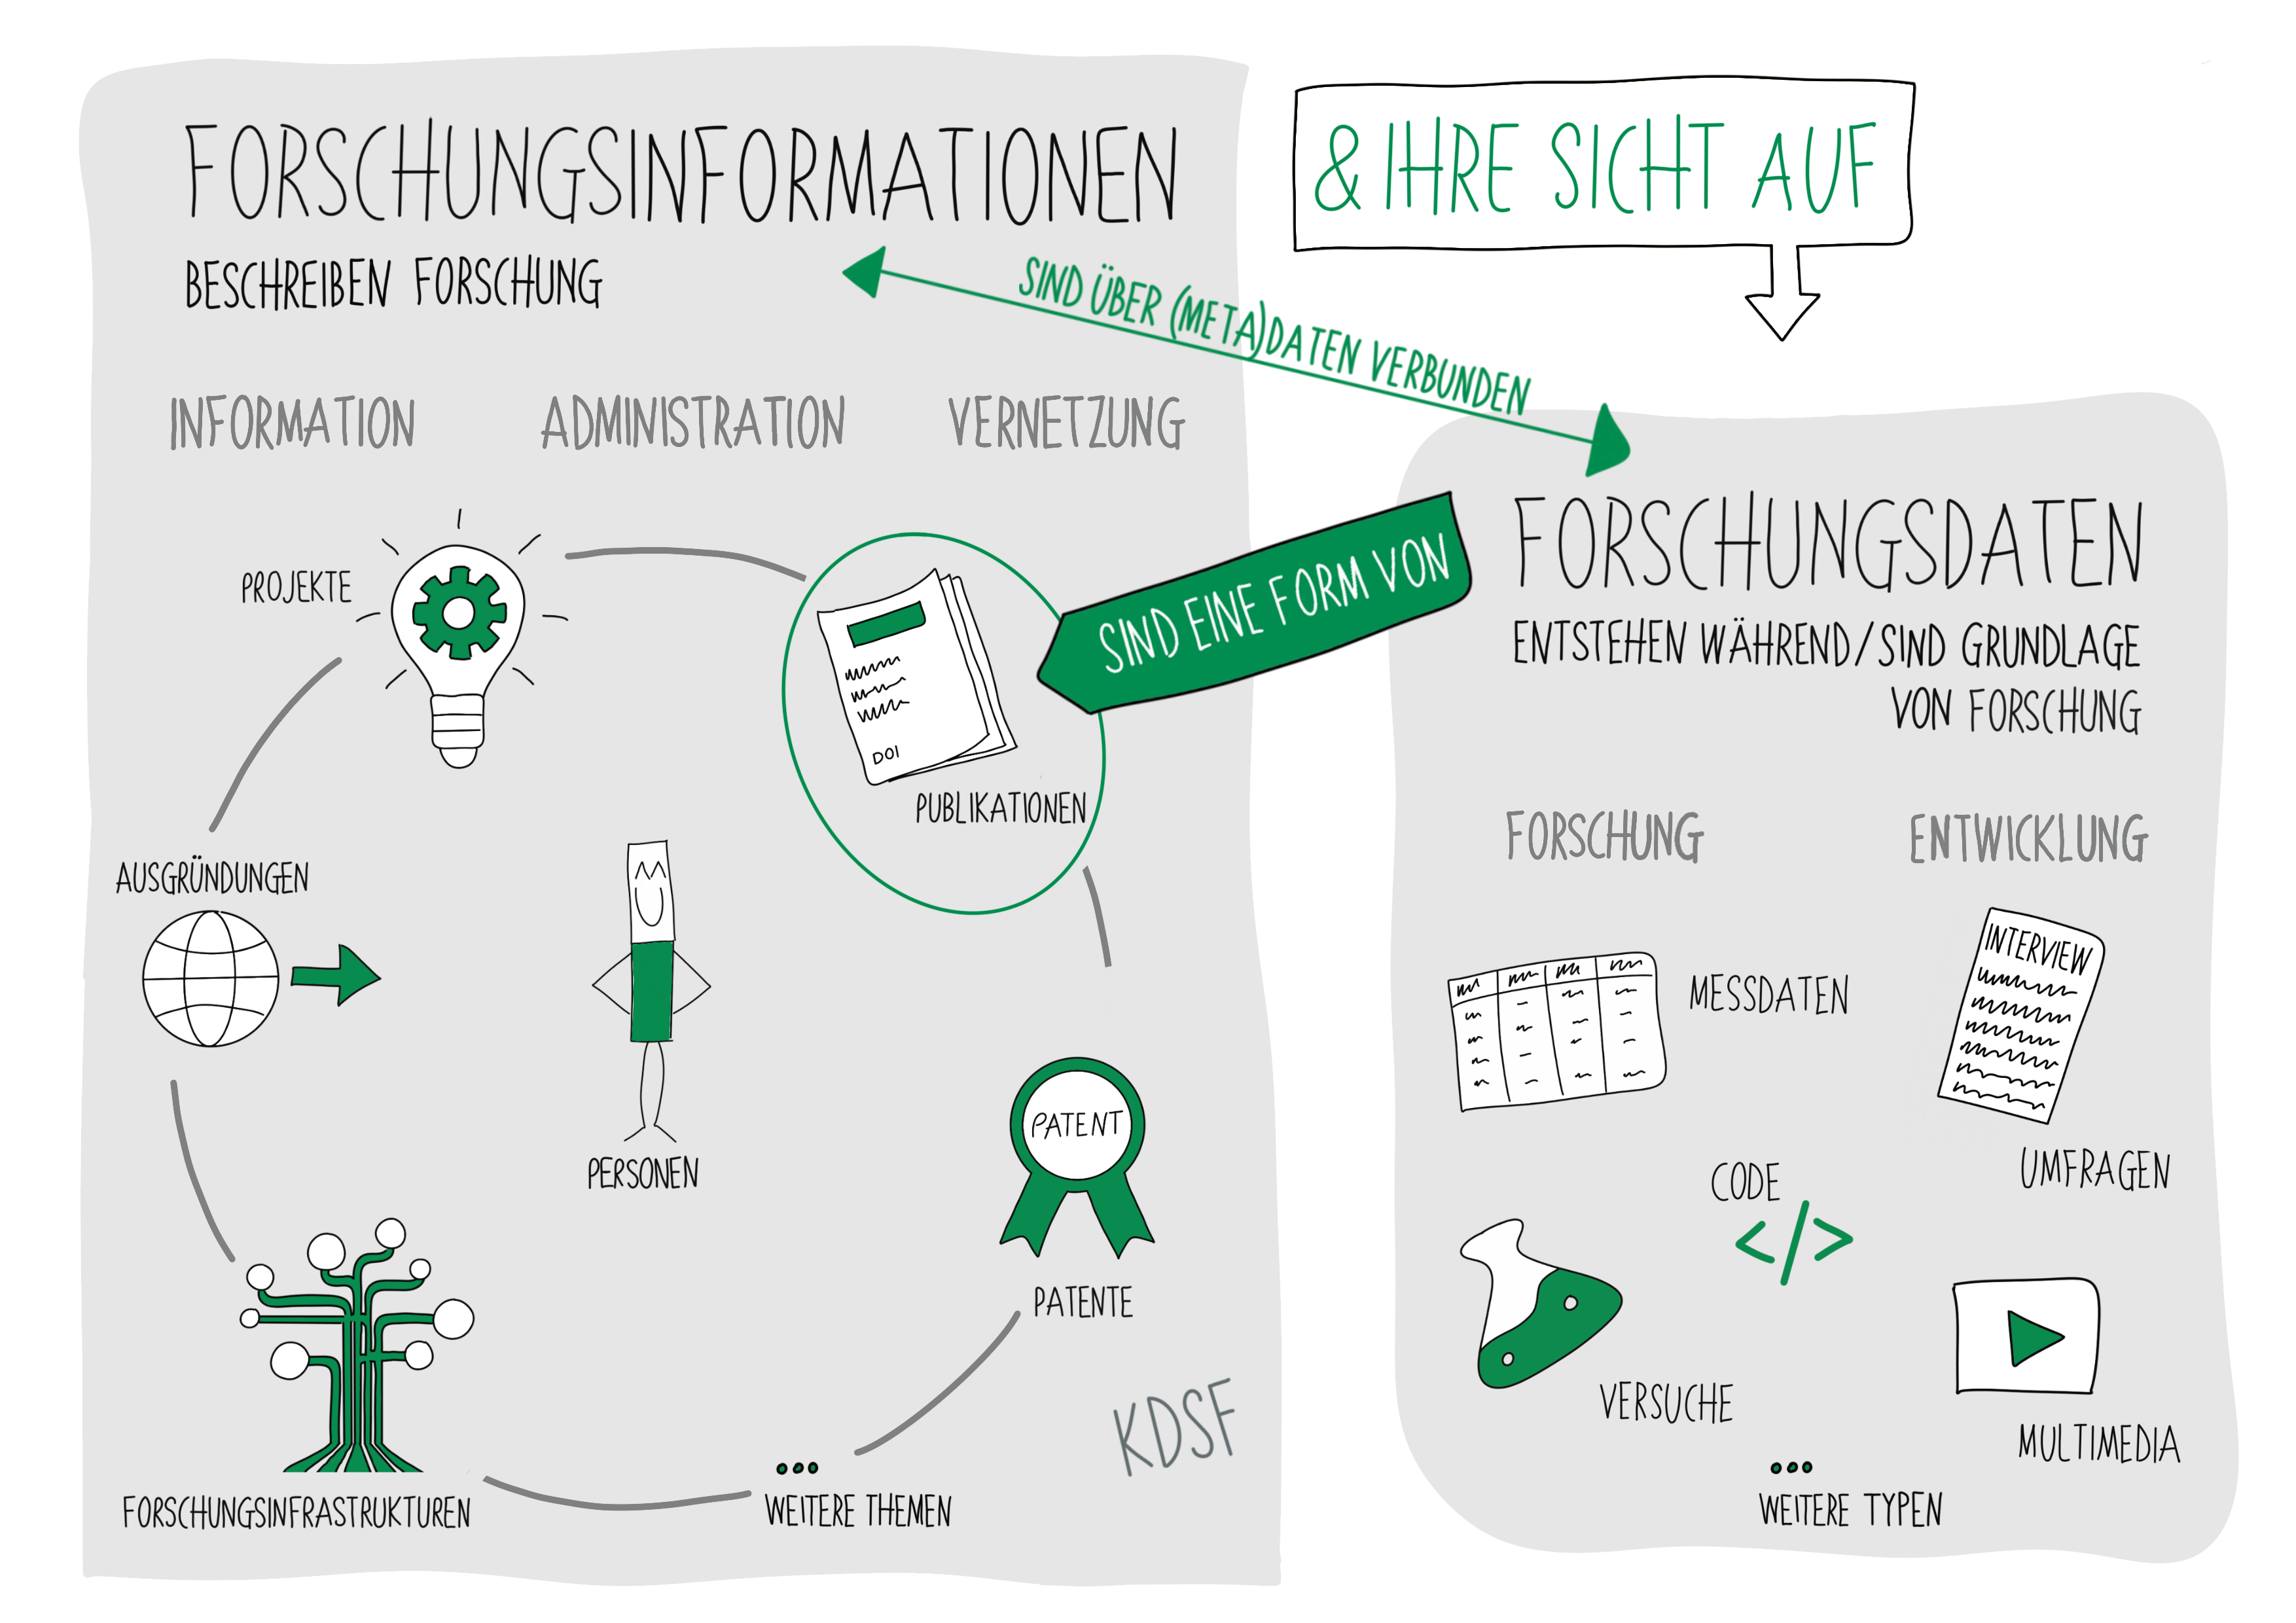
\includegraphics[width=0.95\textwidth,height=\textheight]{media/FIS_FDM_CC_BY_Mau.png}

}

\caption{\label{fig-fis-fdm}Forschungsinformationen und ihre Sicht auf
Forschungsdaten}

\end{figure}%

Services zum Forschungsdatenmanagement ({FDM}) sollen
Wissenschaftler*innen beim Umgang mit ihren Forschungsdaten
unterstützen, und zwar über den gesamten Forschungsdatenlebenszyklus
hinweg, d. h. von der Datenplanung über die Datenerhebung und -analyse
bis hin zur Datenarchivierung, -publikation und -nachnutzung.
Bibliotheken nehmen beim Aufbau und Betrieb entsprechender Services eine
zentrale Rolle ein~-- in aller Regel sind sie hierbei nicht die einzigen
Akteure, sondern das Serviceportfolio wird arbeitsteilig von
Bibliotheken, Rechenzentren, Forschungsabteilungen und ggf.~weiteren
Akteur*innen angeboten. Angesichts der großen Heterogenität
disziplinspezifischer Datentypen gelangen diese in aller Regel
fachübergreifenden {FDM}-Dienste häufig an ihre Grenzen: Diese
Erkenntnis ist konstitutiv für die seit 2020 im Aufbau befindliche
Nationale Forschungsdateninfrastruktur (NFDI), in der fachspezifische
und institutionsübergreifende Dienste entwickelt werden. In diesem
Zusammenhang entwickeln sich derzeit neue Berufe wie Data Steward oder
Data Librarian, die fachspezifische Unterstützung beim {FDM} leisten und
entweder zentral an den {FDM}-Servicestellen oder dezentral in Projekten
oder Fachbereichen angesiedelt sind.

Die von Bibliotheken angebotenen Services zum {FDM} umfassen in der
Regel sowohl nicht-technische Services (z.\,B. Schulungs- und
Beratungsangebote) als auch verschiedene technische Dienste. Zu den
wichtigsten technischen Diensten für das {FDM}, die von Bibliotheken
(mit-)betrieben werden, gehören
\hyperref[repositorien-fuxfcr-forschungsergebnisse]{Repositorien für
Forschungsergebnisse}. Diese ermöglichen die Veröffentlichung von
Forschungsdaten als eigene Informationsobjekte gemäß den FAIR-Prinzipien
Daneben werden häufig weitere {FDM}-Tools angeboten, von denen einige im
Folgenden vorgestellt werden.

\subsection{Tools zur Erstellung von
Datenmanagementplänen}\label{tools-zur-erstellung-von-datenmanagementpluxe4nen}

Um den Umgang mit Forschungsdaten über ein komplettes Projekt zu
beschreiben, hat sich der \textbf{Datenmanagementplan ({DMP})} als
geeignetes Format erwiesen. Derartige Pläne werden zunehmend von
Forschungsförderern bei der Antragstellung oder in der Frühphase des
Projekts erwartet. Sie basieren häufig auf für die Förderlinie bzw.~das
Fachgebiet spezifischen Fragenkatalogen. Durch die einheitlichen
Fragelisten und fest definierte Ausgabeformate lässt sich so ein
menschen- und maschinenlesbares Dokument generieren. Um diese
Fragenkataloge einheitlich zur Verfügung zu stellen und ggf.~mit
einrichtungs- oder programmspezifischen Daten anzureichern, wurden
bereits einige Softwarewerkzeuge entwickelt. In Deutschland verbreitet
ist die in einem von der Deutschen Forschungsgemeinschaft (DFG)
geförderten Projekt entstandene
\href{https://rdmorganiser.github.io/}{Research Data Management
Organizer} (RDMO).

Für diesen werden, unterstützt durch {NFDI}-Konsortien, in einer
Gemeinschaftsarbeit ständig neue Fragenkataloge entwickelt werden.
Obwohl einige öffentliche Instanzen der Software existieren, die z.\,B.
einen Login über die {ORCID} ermöglichen, kann die Open-Source-Software
auch selbst gehostet und inhaltlich sowie visuell auf die Bedarfe der
jeweiligen Einrichtung zugeschnitten werden. {DMP} können innerhalb
dieser Software kollaborativ erstellt werden, indem Personen als
Mitarbeitende in das eigene Projekt eingeladen werden. Für EU-Projekte
ist mit Stand 2023 die Software
\emph{\href{https://argos.openaire.eu/}{ARGOS}} verfügbar, die eine
direkte Einbindung der {DMP} in die \emph{European Open Science Cloud}
(\emph{\href{https://open-science-cloud.ec.europa.eu/}{EOSC}})
ermöglicht. Für Software als Forschungsdatum beginnen sich
Softwaremanagementpläne zu etablieren.

\subsection{Elektronische
Laborbücher}\label{elektronische-laborbuxfccher}

Die Dokumentation der Forschungsergebnisse ist ein zentraler Punkt im
Lebenszyklus von Forschungsdaten. Digital entstandene Daten sollten ohne
Medienbruch mit ihrer Dokumentation verknüpft und zugehörige Metadaten
erfasst werden. Hierzu gibt es eine Reihe dedizierter Softwarelösungen,
die unter dem Begriff elektronische Laborbücher (abgekürzt häufig {ELN}
von \emph{electronic laboratory notebook}) zusammengefasst werden. Neben
kommerziellen Programmen wie
\emph{\href{https://labfolder.com/de/}{LabFolder}}, bei denen
Bibliotheken eher in der Rolle des*der Vermittelnden sind, gewinnen
Open-Source-Lösungen zunehmend an Bedeutung. Diese können Bibliotheken
auf eigenen Servern hosten und selbst administrieren, sind jedoch bei
der Entwicklung neuer Features auf eine Community bzw.~den*die
Entwickler*in oder eigene Fachkräfte angewiesen. Beispiele sind hier
\emph{\href{https://www.elabftw.net/}{eLabFTW}} für generische {ELN}
bzw.~\emph{\href{https://chemotion.net/}{Chemotion}} für eine eher
fachspezifische Lösung. Eine
\href{https://doi.org/10.17192/bfdm.2023.5.8553}{Handreichung zur
Einführung eines {ELN}} an der eigenen Einrichtung wurde 2023 von einer
einrichtungsübergreifenden Autor*innengruppe erstellt. Open Source-{ELN}
erfahren häufig Unterstützung durch {NFDI}-Konsortien. Der daraus
entstandene Wunsch eines einheitlichen Transferformats der
Laborbucheinträge und gemeinsamer Spezifikationen wird im
\emph{\href{https://github.com/TheELNConsortium}{ELN Consortium}}
adressiert. Hilfestellung bei der Auswahl eines passenden Produkts
bietet z.\,B. der
\emph{\href{https://eln-finder.ulb.tu-darmstadt.de/home}{ELN-Finder}}.

\subsection{Git}\label{git}

Als freie Software zur Versionsverwaltung ist \emph{Git} ein
Standardtool der Softwareentwicklung geworden. Durch einfache Befehle
auf der Kommandozeile oder zusätzlich installierte Software mit
grafischem Interface lassen sich textuelle Daten auf dem eigenen System
mit einem externen (Code-)Repositorium abgleichen, das die notwendigen
Protokolle versteht. Neben dem großen Anbieter \emph{GitHub} gibt es die
lokal zu installierende Software \emph{GitLab}, um ein solches
Repositorium in der eigenen IT-Infrastruktur bereitzustellen. Durch die
im Protokoll integrierte Versionskontrolle der Daten lassen sich
Änderungen im Code einfach nachvollziehen und ggf.~zurückrollen.
Kollaborative Arbeit in verteilten Teams wird z.\,B.~über eine parallele
Entwicklungsstruktur in „branches`` ermöglicht, die mit dem Hauptprojekt
zu einem gewünschten Zeitraum zusammengeführt werden können. Bei diesem
Funktionsumfang wird schnell klar, dass \emph{Git} auch jenseits der
forschungsnahen Dienste eine Vielzahl von Anwendungsmöglichkeiten hat.
Die Einbindung in eigene Services wird von Cyra, Politze, und Timm
(2022) am Beispiel der Landesinitiative FDM.NRW erläutert. Eine
Möglichkeit, die Funktion der Software spielerisch zu erkunden, bietet
beispielsweise die vom Bundesministerium für Bildung und Forschung
geförderte Webseite \href{https://ohmygit.org}{ohmygit.org}.

\hyperref[forschungssoftware]{Forschungssoftware} lässt sich, nicht nur
wegen der Verwaltung mit Git oder ähnlichen Programmen, nicht einfach
komplett analog zu den Forschungsdaten behandeln, sondern bedarf eines
genaueren Blicks.

\section{Forschungssoftware}\label{forschungssoftware}

Bei der Betrachtung von Forschungsprozessen setzt sich zunehmend die
Erkenntnis durch, dass auch die dabei zum Einsatz kommende Software ein
Teil der Forschungsdaten ist (Grossmann und Franke (2023)). Dies ist
häufig kein kommerziell erhältliches Produkt, sondern ein speziell auf
das Forschungsproblem zugeschnittener, selbst programmierter Code. Wird
derartige Software nicht korrekt gesichert, versioniert und
dokumentiert, leidet die Reproduzierbarkeit von Forschungsdaten.
Komplexe externe Probleme wie prekäre Beschäftigungsverhältnisse können
zusätzlich zum Verwaisen von Softwareprojekten führen, wenn diese nur
lokal durch einzelne engagierte Personen vorangetrieben wurden.
Zusätzlich führt eine Veröffentlichung der Forschungssoftware zu einer
Auffindbarkeit und Zitierbarkeit, sodass diese zum wissenschaftlichen
Output der Forschenden einen signifikanten Beitrag leisten kann. Aus der
Wissenschaft getriebene Vereinigungen wie
\emph{\href{https://de-rse.org/}{de-RSE e. V.}} treten als Vereinszweck
für den Stellenwert von Forschungssoftware ein. Auch die FAIR-Prinzipien
sollten für Forschungssoftware Anwendung finden (Barker u.~a. (2022)).
Hier liegt es auch an den Bibliotheken, ein Bewusstsein dafür zu
schaffen (z.\,B. durch dedizierte Policies) und die benötigte
Infrastruktur bereitzustellen.

Zur Zitierbarkeit von Forschungssoftware/Code dient die Generierung von
entsprechenden Metadaten, etwa über \url{https://codemeta.github.io/}
und \emph{\href{https://citation-file-format.github.io/}{CITATION.cff}},
um menschen- und maschinenlesbare Zitierinformationen für Software und
Datensätze angeben zu können. Ein entsprechendes Beispiel ist
\href{https://github.com/pro4bib/handbuch-it-in-bibliotheken/blob/main/CITATION.cff}{die
Datei CITATION.cff} im Quelltext dieses Handbuchs.

Die Bereitstellung eines Coderepositoriums, in der Regel über
\emph{Git}, sollte zum Standardangebot zählen. Für eine interaktive
wissenschaftliche Datenauswertung bietet sich zusätzlich der Betrieb
eines \emph{\href{https://jupyter.org/hub}{JupyterHub}} an. Dieser
ermöglicht die Nutzung von Jupyter Notebooks auf einem zentralen Server
der Einrichtung und ist so unabhängig von den jeweiligen
Rechenleistungen der verfügbaren Endgeräte. Zusätzlich sollte geprüft
werden, inwiefern eine Archivierung der Software bzw.~eines gesamten
Repositoriums in der eigenen Infrastruktur nötig und sinnvoll ist.
Anbieter wie \emph{\href{https://www.softwareheritage.org/}{Software
Heritage}} bieten eine Archivierung auf externen Servern an. Zumindest
in diesem Fall ist es als UNESCO-Projekt als geeignete Alternative zu
betrachten.

Die Verknüpfung der im Gesamtprozess entstehenden Metadaten mit Systemen
wie dem Forschungsinformationssystem ({FIS}) oder
Forschungsdatenrepositorien hinsichtlich der Auffindbarkeit dieser
wissenschaftlichen Ergebnisse ist ein Punkt, der eine Betrachtung der
kompletten \hyperref[toolchains]{Toolchain} notwendig macht.

\vfill
\pagebreak

\section{Forschungsinformationssysteme}\label{forschungsinformationssysteme}

\begin{tcolorbox}[enhanced jigsaw, leftrule=.75mm, toprule=.15mm, left=2mm, opacityback=0, arc=.35mm, colback=white, breakable, colframe=quarto-callout-important-color-frame, rightrule=.15mm, bottomrule=.15mm]
\begin{minipage}[t]{5.5mm}
\textcolor{quarto-callout-important-color}{\faExclamation}
\end{minipage}%
\begin{minipage}[t]{\textwidth - 5.5mm}

\textbf{Forschungsinformationen} sind Angaben über Aktivitäten,
Ergebnisse und Infrastrukturen von Forschungsprozessen wie
z.\,B.~Projekte, Publikationen und Forschungseinrichtungen. Davon zu
unterscheiden sind
\hyperref[forschungsdatenmanagement]{Forschungsdaten}.

\end{minipage}%
\end{tcolorbox}

Neben Forschungsdaten gewinnt auch die strukturierte Erfassung von
Forschungsinformationen an Bedeutung. Entsprechende Systeme werden
\textbf{Forschungsinformationssysteme} ({FIS}) genannt. Dabei handelt es
sich um Datenbanksysteme, die speziell für die Erfassung, Organisation,
Speicherung und Verknüpfung von \textbf{Forschungsinformationen}
konzipiert wurden. Sie können interne Anwendungen wie die
leistungsorientierte Mittelvergabe unterstützen und für die
Außendarstellung der Einrichtung genutzt werden. Eine Übersicht von
Forschungsinformationen und ihre Sicht auf Forschungsdaten gibt
Abbildung~\ref{fig-fis-fdm}.

{FIS} führen Informationen zusammen, die dezentral in verschiedenen
hochschulinternen Systemen (z.\,B. Drittmittelverwaltung,
Personalverwaltungssysteme, Repositorien) und externen Quellsystemen (z.
B. \emph{Scopus}, {ORCID}) vorgehalten werden, um einen strukturierten
und aktuellen Überblick über die Forschungsleistungen beispielsweise
einer Einrichtung, eines (Bundes-)Landes oder einer Fachdisziplin zu
gewinnen.

Die genauen Daten, die Nutzung der Daten und der Funktionsumfang eines
{FIS} sind nicht festgelegt bzw.~klar definiert. Verschiedene
Softwarelösungen verfolgen unterschiedliche Ansätze. Bei einige steht
die Auffindbarkeit von Forschungsergebnissen und deren Verknüpfung mit
den Forschenden im Vordergrund, andere Systeme fokussieren eher auf dem
Berichtswesen und Monitoring und ggf. darauf aufbauende Anreizsysteme.
Wiederum andere Systeme legen den Schwerpunkt auf die Präsentation der
Forschungsaktivitäten und deren öffentlichkeitswirksamen Bereitstellung
. Die Systeme passen sich zunehmend aneinander an bzw.~werden die
Funktionen immer häufiger in einem System kombiniert.

{FIS} sollten von Anfang an als Daueraufgabe einer Einrichtung
betrachtet und entsprechende finanzielle und personelle Ressourcen
eingeplant werden. Bei der Einführung eines {FIS} handelt es sich um ein
langjähriges Organisationsentwicklungsprojekt, das eine Offenheit für
Veränderungen in den Prozessen und Workflows der Einrichtung
voraussetzt.

\begin{figure}[H]

{\centering 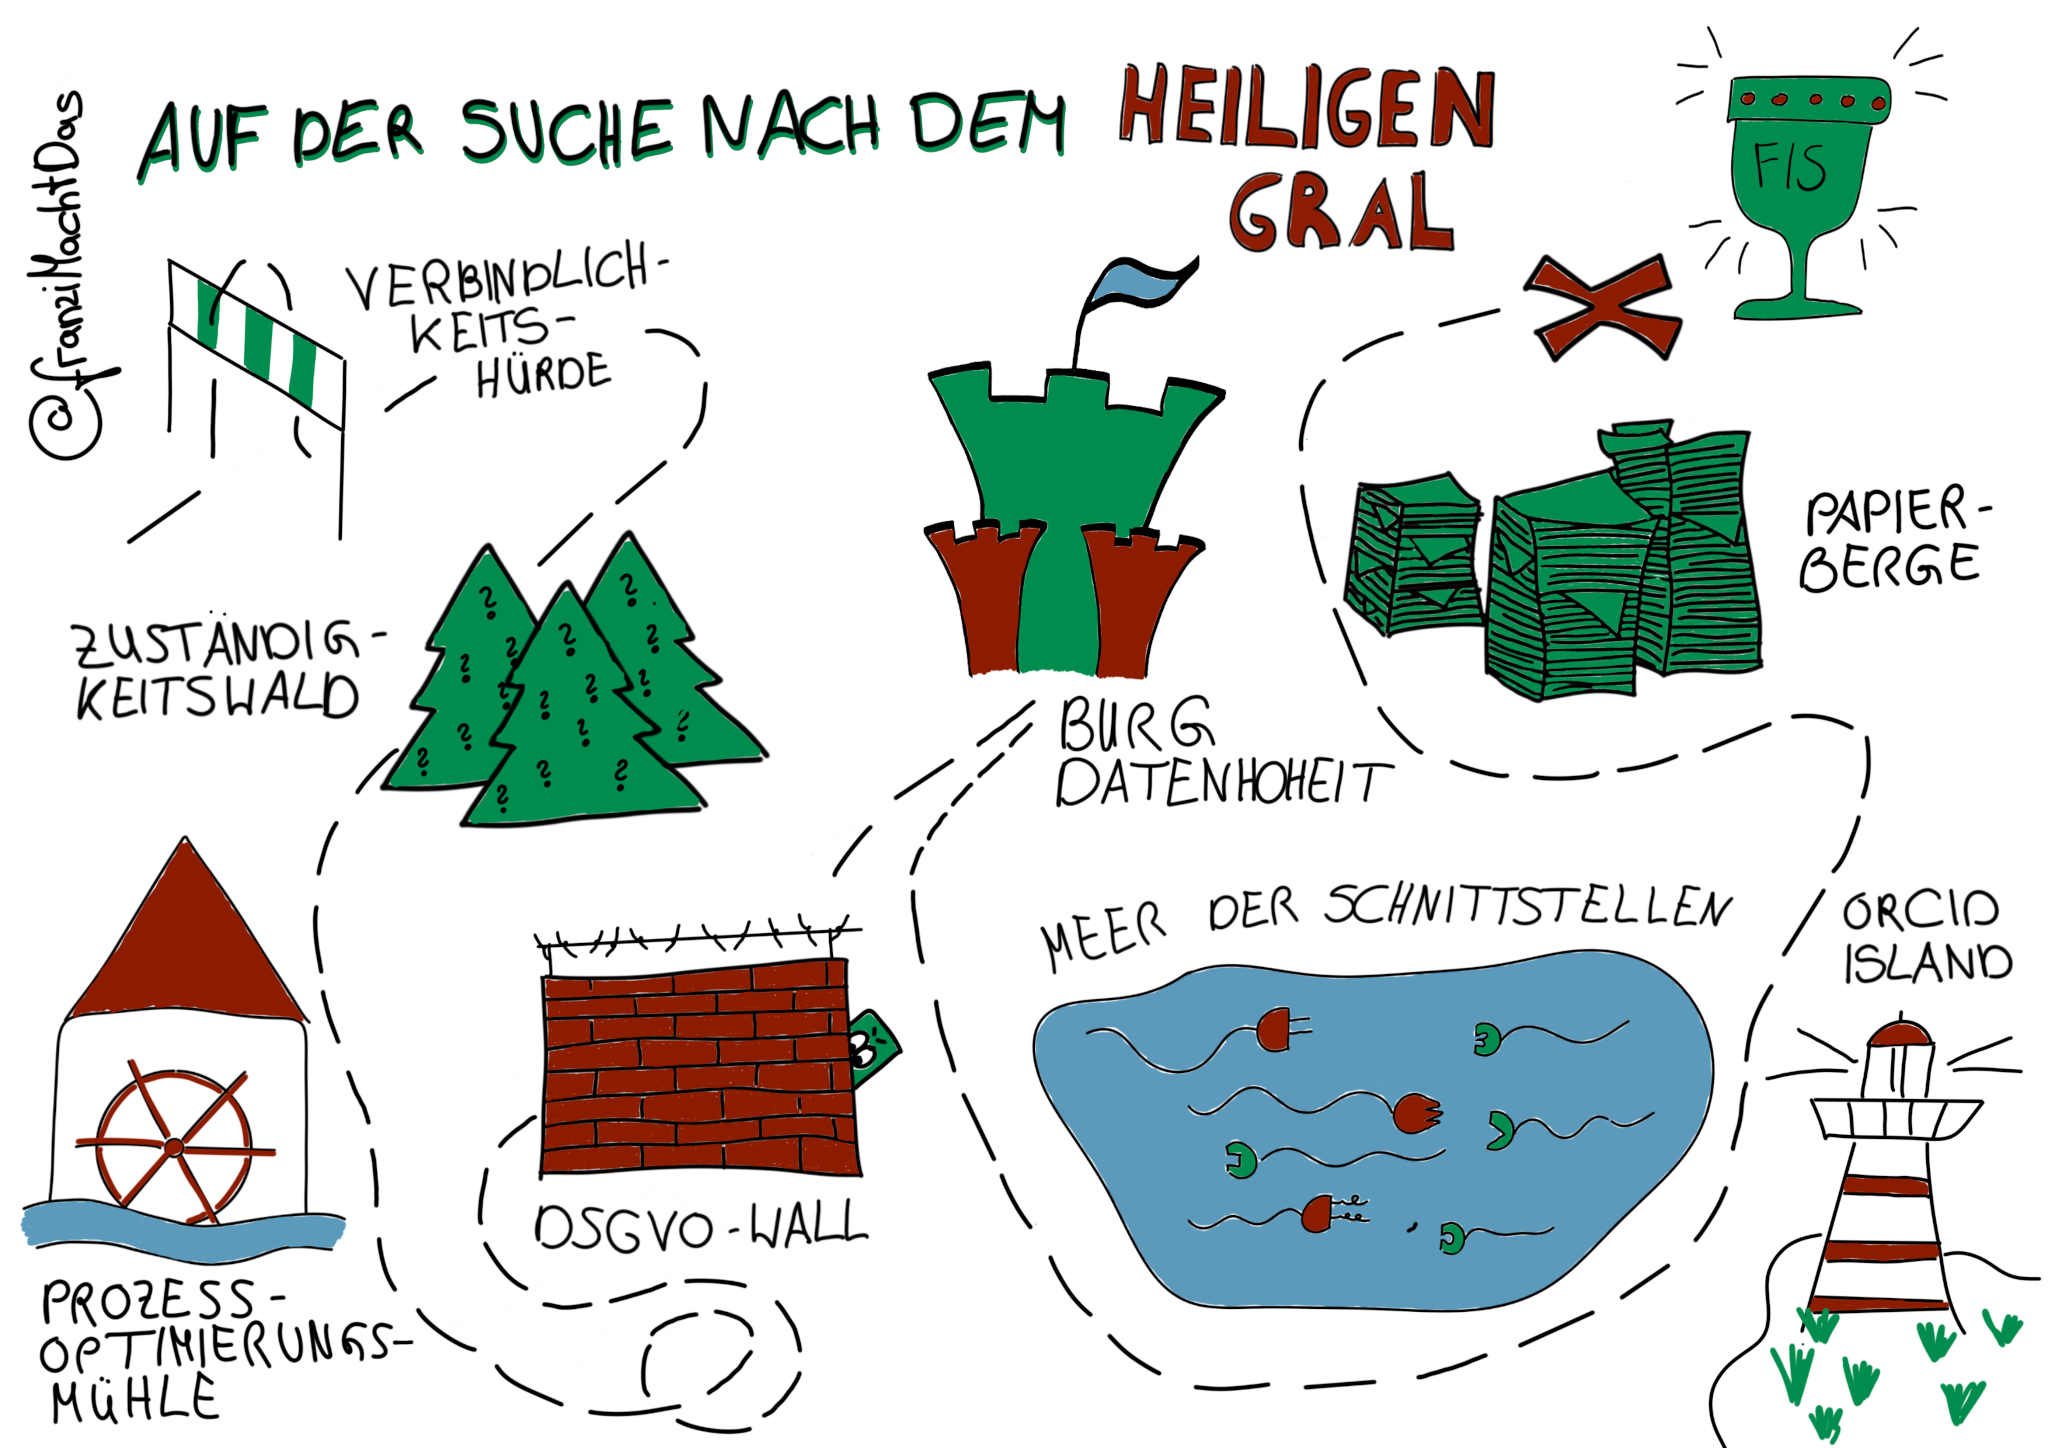
\includegraphics{media/FIS_CC_BY_Mau.png}

}

\caption{Herausforderungen beim Aufbau eines
Forschungsinformationssystem}

\end{figure}%

Eine zentrale Herausforderung beim Aufbau eines {FIS} besteht darin,
einen Überblick über die bestehenden Quellsysteme der Einrichtung zu
gewinnen. In diesem Zusammenhang ist zu ermitteln, welche internen und
externen Systeme relevant sind und wer die entsprechenden
Ansprechpersonen an der Einrichtung sind. Dies betrifft u.\,a.~die
Bibliothek (z.\,B. Repositorien), die Personalverwaltung
(Identitätsmanagement), die Drittmittelverwaltung (Datenbank für
Projekte), die Doktorand*innenverwaltung oder die Patentverwaltung der
Einrichtung.

Neben der Identifikation der relevanten Datenquellen stellt die
Integration der Daten in das {FIS} meist die größte Herausforderung dar.
So muss zum einen für fehlende oder ungeeignete Schnittstellen eine
Lösung gefunden werden. Zum anderen variieren Qualität und Konsistenz
der vorhandenen Daten mitunter stark, was zusätzliche Zeit für die
Datenbereinigung und -konvertierung erfordert. Gleichzeitig ist die
Sicherstellung der Datenintegrität und -qualität von entscheidender
Bedeutung, um zu gewährleisten, dass das {FIS} korrekte und
aussagekräftige Informationen liefert.

Der Markt für {FIS}-Software ist sehr dynamisch. Vor dem Hintergrund,
dass sich gerade viele Forschungseinrichtungen in der Planungs- und
Aufbauphase von {FIS} befinden, kommen in Deutschland immer neue
Softwarelösungen zum Einsatz. Es zeigt sich ein vielgestaltiges Bild aus
kommerziellen Produkten (z.\,B. \emph{PURE}, \emph{Converis},
\emph{HISinOne-RES}), Open Source-Lösungen (z.\,B. \emph{DSpace-CRIS},
\emph{VIVO}) und Eigenentwicklungen. An deutschen
Forschungseinrichtungen wird mittlerweile häufig \emph{HISinOne-RES}
genutzt~-- befördert u.\,a.~durch Landesinitiativen wie \emph{CRIS.NRW},
HeFIS oder \emph{FIS-Thüringen} sowie den Umstand, dass es aktuell das
einzige Produkt am Markt ist, dessen Datenmodell direkt am
\textbf{Kerndatensatz Forschung ({KDSF})} ausgerichtet ist. Obwohl sich
ein Rückgang an Eigenentwicklungen andeutet, sind sie immer noch weit
verbreitet. Des Weiteren gibt es die bereits lange etablierten
kommerziellen Systeme \emph{Converis} und \emph{PURE}. Der Einsatz von
Open-Source-Lösungen wie \emph{DSpace-CRIS} und \emph{VIVO} nimmt erst
in den letzten Jahren merklich zu~-- u.\,a.~befördert durch das
Verbundprojekt Hamburg Open Science.

An vielen Einrichtungen besteht das Bestreben, dass das {FIS} zusätzlich
die Funktionalität eines
\hyperref[repositorien-fuxfcr-forschungsergebnisse]{Repositoriums}
übernehmen soll. Ein Vorteil eines solchen vereinigten Systems wird zum
einen in den geringeren Systemkosten gesehen, zum anderen erscheint es
weniger aufwendig, die bibliografischen Einträge in einem {FIS} schlicht
mit den dazugehörigen Dateien anzureichern statt einen Workflow für das
Zusammenspiel zwischen {FIS} und Repositorium zu entwickeln. Dem
entgegen stehen die verschiedenen Zielsetzungen beider Systeme: Während
es bei einem {FIS} vor allem darum geht, möglichst alle
Forschungsaktivitäten z.\,B. einer Einrichtung in einem System zu
erfassen, steht bei einem Repositorium die nachhaltige Bereitstellung
der Ressourcen selbst im Vordergrund (z.\,B.~textuelle Publikationen
oder Forschungsdaten). Ein Problem bei Mischsystemen ergibt sich auch
hinsichtlich Retrieval und Zugriff: So werden Forschende bei einer Suche
in externen Suchmaschinen z.\,B. erst im {FIS} feststellen, dass nur bei
einem Teil der Treffer tatsächlich Zugang zu den Ressourcen selbst
besteht, sie in den meisten Fällen jedoch lediglich Nachweise der
Ressourcen finden. In der Praxis sind {FIS}-Repositorien-Mischsysteme
dennoch aufgrund von Ressourcenknappheit nicht wegzudenken (Schirrwagen
(2022)).

Nichtsdestoweniger sind die Publikationsdaten ein wichtiger Bestandteil
jedes {FIS}. Aus diesem Grund ist das {FIS} eine gute erste
Anlaufstelle, um interne bibliometrische Recherchen über den Output der
eigenen Forschenden durchzuführen. Darüber hinaus sind primär Anfragen
in externen Datenbanken als ergänzende Arbeitsschritte notwendig.

Um eine Interoperabilität der unterschiedlichen Systeme und eine gute
Auffindbarkeit der enthaltenen Ressourcen zu ermöglichen, ist eine
Standardisierung notwendig~-- z.\,B. über Zertifikate,
\hyperref[metadatenstandards]{Metadatenstandards} und Schnittstellen,
wie sie unter anderem von den Arbeitsgemeinschaften des
\href{https://dini.de/}{DINI e.V.} (Deutsche Initiative
Netzwerkinformation) vorangetrieben werden. Die in diesem Zusammenhang
wichtigen Grundlagen werden in den folgenden Abschnitten erläutert.

\section{Gemeinsame Ressourcen}\label{gemeinsame-ressourcen}

\subsection{Zertifikate und Standards}\label{zertifikate-und-standards}

Forschungsnahe Dienste bewegen sich an der Schnittstelle zwischen
Wissenschaft und Infrastruktureinrichtungen, welche die Dienste
betreiben. Zertifikate erfüllen in diesem Zusammenhang verschiedene
Funktionen. Sie sind als vertrauensbildende Maßnahmen gedacht, die
Qualitätsmerkmale der Dienstleistungen sein sollen. Das
\emph{\href{https://dini.de/dienste-projekte/dini-zertifikat}{DINI-Zertifikat
für Open-Access-Publikationsdienste}} versteht sich seit jeher auch als
Ratgeber bei Einrichtung, Weiterentwicklung und Betrieb solcher
Dienstleistungen, der „Maßstäbe, Richtlinien und Best Practices``
vermitteln will. Letztlich dienen Zertifikate auch dem Schaffen von
Standards, welche die Interoperabilität der Dienste ermöglichen. Neben
dem DINI-Zertifikat sind in Bezug auf forschungsnahe Dienste das
\emph{\href{https://www.coretrustseal.org}{Core Trust Seal}} sowie das
\emph{\href{https://www.langzeitarchivierung.de/Webs/nestor/DE/Zertifizierung/nestor_Siegel/siegel.html}{Nestor-Siegel
für vertrauenswürdige digitale Langzeitarchive}} zu nennen. Während es
mit der DIN Norm 31644 (auch als ISO Norm 16363 verbreitet) „Information
und Dokumentation~-- Kriterien für vertrauenswürdige Langzeitarchive``
eine offizielle Norm für die Bewertung der Vertrauenswürdigkeit von
Langzeitarchiven gibt, werden die meisten Standards in diesem Bereich
eher als Best Practices oder Konventionen, denn als offizielle Normen
eingeführt. Unabhängig von der Frage, ob Zertifikate als
vertrauensstiftend eingeschätzt werden, lohnt es sich, die Dokumentation
der Zertifikate als Ratgeber oder Checkliste zu nutzen; sowohl beim
Aufbau neuer Dienste als auch zur regelmäßigen Überprüfung des eigenen
Dienstes mit Blick auf neue Entwicklungen und Optionen eigene Dienste
weiterzuentwickeln.

Schon im
\emph{\href{http://legacy.earlham.edu/~peters/fos/bethesda.htm}{Bethesda
Statement on Open Access Publishing}} taucht das Stichwort
Interoperabilität in Zusammenhang mit Repositorien auf. Dazu gibt es
verschiedene technische Ansätze (siehe u.\,a.~unten
„\hyperref[schnittstellen]{Schnittstellen}``). Neben den technischen
Voraussetzungen, um Inhalte zu teilen, braucht es jedoch auch eine
Einigung über die inhaltliche Aufbereitung der Informationen.
Repositorien nutzen dazu strukturierte Metadaten. Für die Bezeichnung
von Dokumententypen haben die DINI AG Elektronisches Publizieren und die
DINI AG Forschungsinformationssysteme das
\emph{\href{https://doi.org/10.18452/24147}{Gemeinsame Vokabular für
Publikations- und Dokumenttypen}} herausgegeben. Im Sinne der
Standardisierung enthält das DINI-Zertifikat weitere Vorgaben, wie
z.\,B.~die Klassifizierung nach zumindest den
Dewey-Dezimalklassifikations-Sachgruppen ({DDC}) der Deutschen
Nationalbibliografie und macht Vorgaben an die Ausgestaltung des Open
Archives Initiative Protocol for Metadata Harvesting ({OAI-PMH}). Diese
Standards ermöglichen es Diensten wie z.\,B.~der \emph{Bielefeld
Academic Search Engine} und anderen Aggregatoren Inhalte aus
verschiedenen Quellen einzubinden, Metadaten maschinenlesbar zu erhalten
und nachzunutzen.

\subsection{Metadaten}\label{metadaten}

Metadaten sind Daten struktureller, technischer, administrativer,
bibliografischer und deskriptiver Natur, die Daten beschreiben
(Kapitel~\ref{sec-metadaten}).
\hyperref[metadatenstandards]{Metadatenstandards und -schemas}
definieren, welche Inhalte in Metadaten erfasst werden, also welche
Metadatenfelder existieren und mit Werten belegt werden können. Ein sehr
einfaches Metadatenschema bilden die
\href{https://www.dublincore.org/specifications/dublin-core/usageguide/elements/}{Dublin
Core Element} (kurz \emph{Dublin Core}). Im Rahmen der DOI-Registrierung
werden auch Metadaten erhoben. Das
\emph{\href{https://schema.datacite.org}{DataCite Schema}} hat sich
dabei als ein wichtiges Metadatenschema etabliert, das auch unabhängig
von DOIs zur Beschreibung von Forschungsdaten genutzt wird. Darüber
hinaus entwickeln die verschiedenen Fachdisziplinen eigene
domänenspezifische Standards. Eine Aufgabe wissenschaftlicher
Bibliotheken besteht in der Beratung bei der Auswahl geeigneter
Metadatenschemata und Standards. Übersichten gibt es unter anderem bei
\href{https://fairsharing.org/search?fairsharingRegistry=Standard}{FAIRsharing.org},
\href{https://www.forschungsdaten.info/themen/beschreiben-und-dokumentieren/metadaten-und-metadatenstandards}{forschungsdaten.info}
und \href{https://format.gbv.de/}{format.gbv.de}.

\subsection{Persistent Identifier}\label{persistent-identifier}

Mit dem Aufkommen elektronischer Archive kam die Frage nach der
Zitierbarkeit auf. Auch wenn die technischen Protokolle, auf denen das
Internet basiert, sowohl im Domain Name System ({DNS}) als auch http(s)
Mechanismen enthalten, um URLs weiterzuleiten, bekamen URLs schnell den
Ruf, flüchtig zu sein. Auch wenn URLs, die nicht mehr oder auf andere
Inhalte auflösen, immer auf Managementprobleme zurückgehen, wurden
\emph{Persistent Identifier}-Systeme geschaffen, welche diese Probleme
beim Zitieren elektronischer Quellen überwinden sollen. Dabei werden IDs
geschaffen, die über einen sogenannten Resolver aufgelöst werden können.
Der Resolver ist vergleichbar mit einem Melderegister: Man kann nach der
aktuellen Adresse einer ID fragen und erhält die jeweils aktuelle URL
zurück, unter der sich die Ressourcen befinden sollen. Die Antworten
können also zu unterschiedlichen Zeitpunkten unterschiedlich ausfallen.

Während die Deutsche Nationalbibliothek (DNB) bis heute auf URN:NBN als
\emph{Persistent Identifier} ({PID}) setzt, haben sich im
wissenschaftlichen Umfeld DOIs für die Identifikation von Artikeln,
Daten und anderen Inhalten durchgesetzt. In Deutschland kommen dabei vor
allem die DOI-Registrierungsagenturen
\emph{\href{https://datacite.org}{DataCite}} und
\emph{\href{https://www.crossref.org/}{CrossRef}} zum Einsatz. Beide
vergeben DOIs sowohl für textuelle Publikationen als auch für Datensätze
und andere Inhalte. Von der technischen Einbindung her ist
\emph{DataCite} moderner aufgestellt und leichter zu integrieren. Mit
{ORCID} und \emph{\href{https://ror.org}{ROR}} gibt es inzwischen
weitere PID-Systeme, die zunehmend Verbreitung finden und Personen
bzw.~Einrichtungen eindeutig identifizieren.

Die Vergabe von PIDs für Publikationen (z.\,B. Texte, Forschungsdaten)
auf Publikationsservern bzw.~Datenrepositorien wird teilweise von den
wissenschaftlichen Bibliotheken gewährleistet. Somit werden
Forschungsdaten nachhaltig unter entsprechenden Lizenzen öffentlich
verfügbar gemacht (Berg-Weiß et al. 2022). Mit dem Ziel, eine nationale
Beratungs- und Austauschplattform zu PID aufzubauen, fördert die DFG
seit 2023 das Projekt ``\href{https://www.pid-network.de/}{PID Network
Deutschland}.

\subsection{Langzeitarchivierung}\label{langzeitarchivierung}

Die dauerhafte Aufbewahrung und Lesbarkeit von digitalen Objekten zu
gewährleisten, stellt auch für Bibliotheken, die zunehmend für die
Archivierung von Open-Access-Publikationen, Forschungsdaten und anderen
elektronischen Ressourcen verantwortlich sind, eine große
Herausforderung dar. Die sogenannte \textbf{digitale
Langzeitarchivierung ({LZA})} beinhaltet neben der Speicherung
zusätzliche Maßnahmen wie die regelmäßige Überprüfung der
Datenintegrität, die Migration der Daten auf neue Speichermedien und die
Anpassung an sich verändernde Technologien. Digitale Informationen
bleiben so langfristig erhalten und auch in der Zukunft zugänglich.

Bewahrt werden müssen der Bitstream der Datei sowie deren Eigenschaften
und Semantik. Aktuell ist
\emph{\href{https://www.loc.gov/standards/premis/}{PREMIS}} in der {LZA}
der wichtigste Metadatenstandard. Das Datenmodell beinhaltet alle
Informationen, die man sowohl über die digitalen Objekte selbst
(z.\,B.~Name, Dateiformat, Größe) als auch über Akteur*innen, Rechte
(z.\,B.~AccessRights, Embargofristen) und Prozesse
(z.\,B.~Konvertierung, Migrationen, Reparatur, Formatvalidierung) wissen
sollte.~

Es gibt auf {LZA} spezialisierte Software wie \emph{Rosetta}
(\emph{ExLibris}) oder \emph{Libsafe} (\emph{libnova}). Diese Systeme
basieren meist auf dem international anerkannten Referenzmodell für
digitale Archivierung \emph{OAIS}
(\emph{\href{https://www.iso.org/standard/87471.html}{Open Archival
Information System, ISO 14721:2025}}) und bieten neben den
Standardfunktionen eines Archivsystems (z.\,B.~bitstream-preservation,
regelmäßige Integritätstests, Reduplizierung) auch Funktionen wie eine
Formatvalidierung und implementierbare Workflows.

Auf der Webpage \href{https://coptr.digipres.org/}{COPTR}~-- Community
Owned digital Preservation Tool Registry~-- werden diese und zahlreiche
weitere Tools und Workflows zur {LZA} vorgestellt. Als wichtige
Anlaufstelle für Fragen rund um die digitale {LZA} dient außerdem das
\emph{\href{https://www.langzeitarchivierung.de/}{Kompetenznetzwerk
nestor}}, dessen Geschäftsstelle an der DNB angesiedelt ist. Auch die
{NFDI}
behandelt~„\href{https://doi.org/10.5281/zenodo.6451456}{Long-term
Archival (LTA)}`` in der
\href{https://www.nfdi.de/section-infra/}{Sektion „Common
Infrastructures``} als Querschnittsthema.

\begin{figure}

\centering{

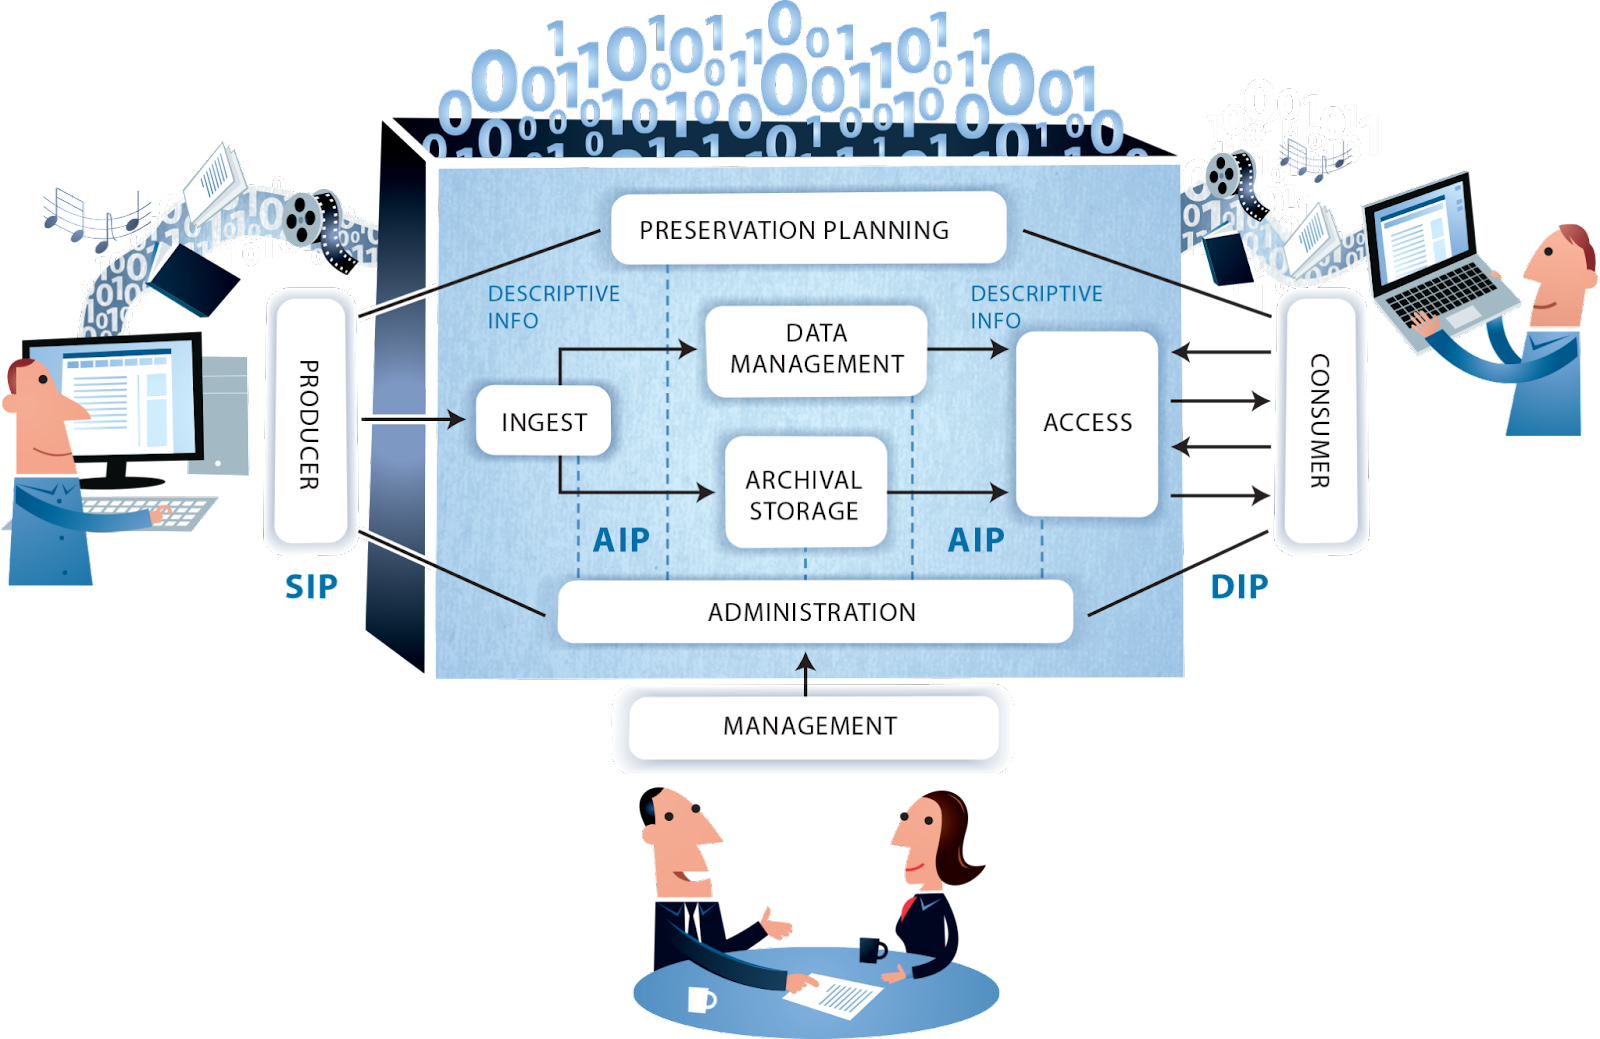
\includegraphics{media/oais.png}

}

\caption{\label{fig-oais}Das als ISO 14721 verabschiedete Referenzmodell
„Open Archival Information System'' (OAIS)}

\end{figure}%

\subsection{Schnittstellen}\label{schnittstellen-1}

Einen allgemeinen Überblick zu Schnittstellen liefert das
Kapitel~\ref{sec-metadaten}. Im Folgenden gehen wir etwas ausführlicher
auf die wichtigsten Schnittstellen im Kontext forschungsnaher Dienste
ein.

Im Bereich von Repositorien hat sich das
\emph{\href{https://www.openarchives.org/pmh/}{Open Archives Initative
Protocol for Metadata Harvesting}} ({OAI-PMH}) für den Austausch von
Metadaten durchgesetzt. Dieses Protokoll wird inzwischen auch im
Zusammenspiel mit anderen forschungsnahen Diensten wie z.\,B.~{FIS}
genutzt. Das Protokoll tauscht Metadaten in XML aus. Es unterstützt
mehrere Metadatenformate, wobei die Spezifikation von {OAI-PMH} nur
\emph{Dublin Core} vorgibt und das Protokoll vorsieht, dass man eine
Liste mit weiteren unterstützten Formaten abrufen kann.

Für das Einbringen von Daten in Repositorien hat sich das Protokoll
\emph{\href{https://swordapp.org/}{Simple Webservice Offering Repository
Deposit}} ({SWORD}) durchgesetzt, wobei auf die genaue Version dieses
Standards geachtet werden muss. Einige Open-Access-Verlage bieten an,
Dokumente über {SWORD} direkt in Repositorien zu übertragen.
\emph{\href{https://info.oa-deepgreen.de/}{DeepGreen}}, ein Lieferdienst
für Open-Access-Artikel, versorgt Repositorien über {SWORD} mit
Verlagsinhalten.

Speziell für die Arbeit mit Bildern, Bildviewern und Bilddatenbanken
wurde das \emph{International Image Interoperability Framework (IIIF)}
entwickelt. IIIF deckt umfangreich verschiedene Funktionen ab, wie die
Ausgabe von Bildern in verschiedenen Formaten und Auflösungen oder
Zoomstufen, die strukturelle Beschreibung von Bildern, Suchanfragen in
einem Bildpool, Umgang mit Zugriffsbeschränkungen, Objektänderungen und
so weiter.

{OAI-PMH} und {SWORD} werden zum Teil zwar auch über Repositorien hinaus
verwendet, z.\,B.~bei {FIS}. Verbreitung und Einsatz beschränken sich
jedoch weitgehend auf den Bereich der forschungsnahen Dienste. Als
weiter verbreitete Prinzipien zur Bereitstellung von Informationen muss
\emph{Linked Data} gesehen werden. Die Bereitstellung der
Repositorieninhalte als \emph{Linked Data} wird z.\,B. von \emph{DSpace}
unterstützt, in der Praxis jedoch leider noch viel zu selten aktiviert
und genutzt.

Allgemein verbreiten sich derzeit \emph{REST}-Schnittstellen, also
Schnittstellen zur Einbindung von Diensten über das Internet in
verschiedene Programme und Infrastrukturen. Auch forschungsnahe Dienste
profitieren sehr von der Bereitstellung von \emph{REST}-Schnittstellen,
damit sie miteinander verschränkt und in andere Infrastrukturen
eingebunden werden können.

Im Bereich von Repositorien, der in Bezug auf Schnittstellen und
Standards oft Auswirkungen auf andere forschungsnahe Dienstleistungen
hat, wurden von der
\emph{\href{https://www.coar-repositories.org/}{Coalition of Open Access
Repositories}} (\emph{COAR}) weitere neue Protokolle vorgeschlagen.
Hierzu zählt Signposting, das typisierte Links einsetzt, um von einer
Ressource auf andere in Verbindung stehende Ressourcen zu verlinken und
so die Auffindbarkeit durch Crawler und Bots erleichtern soll. Derzeit
ist offen, ob Signposting sich durchsetzt. Wenn möglich, sollte es in
Repositorien aktiviert werden.

Eine aktuelle Entwicklung ist das
\emph{\href{https://www.coar-repositories.org/notify/}{Notify Project}},
das ebenfalls von \emph{COAR} betrieben wird. \emph{Notify} soll es
ermöglichen, dass sich verschiedene forschungsnahe Dienste Nachrichten
über Aktivitäten senden und so auf Ressourcen aufmerksam machen. Als
Beispiele gelten automatisiert ablaufende Aktivitäten zwischen einem
textuellen Repositorium und einem Forschungsdatenrepositorium oder
zwischen einem Repositorium und einem Service für die Organisation des
Peer-Reviewing. \emph{Notify} hat vor allem in den USA eine größere
Förderung erhalten und wird derzeit in Softwarelösungen für verschiedene
forschungsnahe Dienste integriert. Es ist zu erwarten, dass
\emph{Notify} sich in diesem Bereich verankern und helfen wird, Dienste
dynamischer miteinander zu verknüpfen.

Von diesen Entwicklungen wird auch die Veröffentlichung von
Forschungsdaten profitieren. Bevor Daten allerdings in einem Zustand
sind, dass sie veröffentlicht werden können, durchlaufen sie einen
eigenen Lebenszyklus, bei dem unterstützende Dienste der Bibliotheken
zunehmend gefragt sind.

\subsection{Toolchains}\label{toolchains}

\begin{tcolorbox}[enhanced jigsaw, leftrule=.75mm, toprule=.15mm, left=2mm, opacityback=0, arc=.35mm, colback=white, breakable, colframe=quarto-callout-important-color-frame, rightrule=.15mm, bottomrule=.15mm]
\begin{minipage}[t]{5.5mm}
\textcolor{quarto-callout-important-color}{\faExclamation}
\end{minipage}%
\begin{minipage}[t]{\textwidth - 5.5mm}

Eine \textbf{Toolchain} („Werkzeugkette``) ist eine Reihe von
miteinander verbundenen Anwendungen und Technologien, die gemeinsam
eingesetzt werden, um spezifische Aufgaben oder Arbeitsabläufe zu
optimieren und zu automatisieren. Die Einrichtung einer Toolchain hilft,
den reibungslosen Informationsfluss zwischen Arbeitsschritten zu
verbessern.

\end{minipage}%
\end{tcolorbox}

Forschungsnahe Dienste müssen immer im Kontext des Forschungsprozesses
und im Hinblick auf den Nutzen für die Forschenden betrachtet werden.
Dazu ist es wichtig, für jeden der Dienste, die an einer Einrichtung
genutzt werden, ein klares Profil zu erstellen. Hierbei muss
insbesondere geklärt werden, wie sich die Dienste voneinander abgrenzen,
damit Nutzenden klar kommuniziert werden kann, welcher Dienst wofür
verwendet wird.

Gleichzeitig muss auch das Zusammenspiel der einzelnen Dienste
analysiert werden. Wie knüpfen die verschiedenen Dienste aneinander an?
Wie kann der gebotene Mehrwert durch Verknüpfungen der Dienste
gesteigert werden? Welche Dienste bauen wie aufeinander auf? Diese
Fragen sind nur lokal und konkret zu vorhandenen oder in Planung
befindlichen Diensten zu beantworten.

Beispiel: An einer Bibliothek findet in Zusammenarbeit mit
Fachwissenschaftler*innen ein großes Retro-Digitalisierungsprojekt
statt. Für die Verwaltung der
\hyperref[digitalisierung]{Digitalisierungsvorgänge} wird \emph{Kitodo}
verwendet. Die Werke sind im BMS verzeichnet und die Metadaten werden
über die Search/Retrieve via URL-Schnittstelle ({SRU}) nach
\emph{Kitodo} importiert. Weitere Strukturdaten werden in \emph{Kitodo}
direkt eingetragen. Nach dem Scannen werden die Dokumente von
\emph{Kitodo} über die \emph{REST-API} oder {SWORD} in das Repositorium
exportiert. Das Repositorium ruft weitere Metadaten über {SRU} aus dem
Bibliothekskatalog ab und vergibt DOIs, die wieder in das BMS
zurückgespeichert werden. Das {FIS} harvestet die Inhalte über {OAI-PMH}
regelmäßig und weist die Digitalisate nach, die im Repositorium
bereitgestellt werden.

In diesem ideellen Bild wird nicht betrachtet, wo die nötigen Systeme
stehen. Dies muss nicht immer ein lokal betriebenes System auf eigener
Hardware sein, sondern ist oftmals als externer Service verfügbar.

\subsection{Zusammenarbeit mit
Dienstleistern}\label{zusammenarbeit-mit-dienstleistern}

Selbstverständlich ist es nicht bei allen Problemstellungen möglich,
IT-Services für forschungsnahe Dienste im eigenen Haus anzubieten. Bei
bereits etablierten Anwendungen lohnt sich eine Kontaktaufnahme mit der
jeweiligen Verbundzentrale. Häufig werden dort bereits Services
angeboten, für die man kein zusätzliches Personal bzw.~keine eigene
Infrastruktur einplanen muss. Wird die Verwendung einer bestimmten
Software gefordert oder eine bestimmte Art, die Software einzusetzen,
die nicht im Dienstleistungsportfolio der Verbundzentralen liegt, bietet
sich die Zusammenarbeit mit externen, kommerziellen Dienstleistern an.
Wo immer möglich, sollte Software von Open Source-Communities Vorrang
vor proprietärer Software genießen, da sie vor Abhängigkeiten von
einzelnen Anbietern schützt und Weiterentwicklungen, welche in die
Community eingebracht werden, von anderen Einrichtungen wiederverwendet
werden können. Vor allem im Bereich der forschungsnahen Dienste sind
Open Source-Lösungen oft vorherrschend. Ziel von
Infrastruktureinrichtungen sollte es sein, das zu erhalten, anstatt den
Aufbau proprietärer Software und neuer Oligopol- oder Monopolstellungen
zuzulassen. Der Mehrwert, den IT-Dienstleister bieten, besteht ähnlich
wie bei den Verbundzentralen darin, dass man selbst personelle und
ggf.~Infrastrukturressourcen sparen kann. In den meisten Fällen gibt es
die Möglichkeit, entweder die Installation und Betreuung des Dienstes
auf lokaler Infrastruktur oder auch ein „Rundum-Sorglos-Paket`` mit
Hosting beim Dienstleister inklusive Betreuung einzukaufen.

Bei der Wahl des Anbieters gilt es, auf dessen Erfahrung im Umgang mit
Open Source-Projekten allgemein und mit der gewünschten Software im
Speziellen zu achten. Genau wie sich nach Referenzen zu vergleichbaren
Projekten zu erkundigen, lohnt es sich, nach konkreten bereits
geleisteten Beiträgen zu der jeweiligen Open Source-Lösung zu fragen.
Wenn die Open Source-Lizenzen der jeweiligen Software keine Auflage
machen, dass Weiterentwicklungen unter derselben Lizenz verbreitet
werden müssen, sollte die Frage, unter welcher Softwarelizenz
Weiterentwicklungen stehen, zwingend im Vertrag geklärt werden.

Besonders weit verbreitete Softwarelösungen haben große
Entwicklergemeinschaften, die es einerseits zu unterstützen gilt,
andererseits ist auch die Communitygetriebene Entwicklungsrichtung der
Software zu beachten. Ist der gewünschte Dienstleister noch neu, ist
zumindest eine anderweitige Erfahrung in ähnlichen Projekten
wünschenswert. Eine Recherche in öffentlichen Software-Repositorien der
Projekte kann hier zielführend sein.

\section{Zusammenfassung und
Ausblick}\label{zusammenfassung-und-ausblick-5}

Forschungsnahe Dienste können Wissenschaftler*innen grundsätzlich über
den gesamten Forschungsprozess hinweg unterstützen~-- das Portfolio
möglicher Services ist daher sehr groß. Bibliotheken setzen ihren
Schwerpunkt hierbei insbesondere auf Services zur Unterstützung des
Publikationsprozesses sowie des FDM.

Selbstverständlich ist es nicht bei allen Problemstellungen möglich,
IT-Services für forschungsnahe Dienste im eigenen Haus anzubieten. Bei
bereits etablierten Anwendungen lohnt sich eine Kontaktaufnahme mit der
jeweiligen Verbundzentrale. Häufig werden dort bereits Services
angeboten, für die man kein zusätzliches Personal bzw.~keine eigene
Infrastruktur einplanen muss. Beispiele hierfür sind der
Repository-Service
\emph{\href{https://www.gbv.de/informationen/Verbundzentrale/serviceangebote/reposis-repository-service}{Reposis}}
des GBV oder das Langzeitarchiv \emph{\href{https://ewig.zib.de/}{Ewig}}
des KOBV. Die Frage nach der Umsetzung von Diensten mit externer Hilfe
allgemein wird in Kapitel~\ref{sec-management} behandelt.

Wie das vorliegende Kapitel gezeigt hat, umfassen diese Services auch
eine Vielzahl an IT-Diensten, so z.\,B. Journal-Publishing-Systeme,
Repositorien und {FIS}. Der stabile und nachhaltige Betrieb solcher
Dienste umfasst technische, organisatorische und inhaltliche Aspekte.
Der Aufbau und Betrieb forschungsnaher Dienste an Bibliotheken bindet
daher umfangreiche Ressourcen und erfordert ggf.~auch eine Verlagerung
von Ressourcen aus anderen Bereichen. Die Ausweitung des
bibliothekarischen Serviceportfolios um forschungsnahe Dienste ist daher
auch eine Frage der Organisations- und Personalentwicklung.

\bookmarksetup{startatroot}

\chapter{Kommunikation}\label{sec-kommunikation}

\begin{tcolorbox}[enhanced jigsaw, leftrule=.75mm, toprule=.15mm, left=2mm, opacityback=0, arc=.35mm, colback=white, breakable, colframe=quarto-callout-note-color-frame, rightrule=.15mm, bottomrule=.15mm]
\begin{minipage}[t]{5.5mm}
\textcolor{quarto-callout-note-color}{\faInfo}
\end{minipage}%
\begin{minipage}[t]{\textwidth - 5.5mm}

\vspace{-3mm}\textbf{Zusammenfassung}\vspace{3mm}

Bibliotheken bedienen verschiedene Kommunikationsräume. Für die
\hyperref[ziele]{interne und externe Kommunikation} stehen verschiedene
\hyperref[prozesse]{Prozesse}, \hyperref[kanuxe4le]{Kanäle} und
\hyperref[werkzeuge]{Werkzeuge} zur Verfügung.

\end{minipage}%
\end{tcolorbox}

\section{Einleitung}\label{einleitung-9}

Im Verhältnis zwischen Intranet und Öffentlichkeitsarbeit bewegt sich
die moderne Bibliothekslandschaft zunehmend weg von einem dualen
Kommunikationsverständnis hin zu einem integrierten Ansatz. Dabei
überlappen Kommunikationsräume oft. Werkzeuge dienen sowohl der internen
Kommunikation als auch dem Dialog mit der Öffentlichkeit.

Indem Bibliotheksmitarbeitende aktiv mit Intranettools und -plattformen
arbeiten, bauen sie technische Fähigkeiten und Selbstvertrauen im Umgang
mit ähnlichen Kommunikationswerkzeugen für die externe Kommunikation
auf. Dadurch wird die Einführung von Intranetwerkzeugen zu einer
Schlüsselstrategie der Organisationsentwicklung. Mitarbeitende
verwandeln sich so in authentische Botschafter der digitalen
Transformation, interagieren kompetent und auf Augenhöhe mit den
Nutzenden und verkörpern eine innovative, nutzerzentrierte
Kommunikationsweise:

\begin{figure}

\centering{


\includegraphics{index_files/mediabag/media/stufenmodell.pdf}

}

\caption{\label{fig-stufenmodell}Stufenmodell von Öffentlichkeitsarbeit}

\end{figure}%

\section{Ziele}\label{ziele}

Das Stufenmodell macht deutlich, dass der Übergang von einem internen zu
einem externen Publikum ein Kontinuum darstellt. Dennoch lassen sich die
\textbf{\hyperref[ziele-interner-kommunikation]{Ziele interner}} und
\textbf{\hyperref[ziele-externer-kommunikation]{externer Kommunikation}}
klar voneinander abgrenzen.

\subsection{Ziele interner
Kommunikation}\label{ziele-interner-kommunikation}

\textbf{Interne Kommunikation} bezieht sich auf den gezielten Austausch
von Informationen, Meinungen und Vorstellungen innerhalb einer
Organisation. Sie umfasst sämtliche Kommunikationsprozesse und
-instrumente, die darauf abzielen, die Mitarbeiter:innen eines
Unternehmens oder einer Einrichtung miteinander und mit der Organisation
insgesamt zu vernetzen. Hauptziele sind oft die Sicherstellung eines
konsistenten Informationsflusses, die Unterstützung der
organisatorischen Ziele und die Förderung einer positiven
Unternehmenskultur. Im besten Falle vermeidet gelungene interne
Kommunikation Wissensinseln und zu starke Wissensbindung an einzelne
Personen.

\textbf{Wissensmanagement} beschreibt hingegen den Prozess des
Erfassens, Organisierens, Bewahrens, Anwendens und Weitergebens von
Wissen innerhalb einer Organisation. Dieses Wissen kann sowohl explizit
(in Dokumenten, Datenbanken etc.) als auch implizit (in den Köpfen der
Mitarbeitenden) vorhanden sein. Das Wissensmanagement zielt darauf ab,
das im Unternehmen vorhandene Wissen effektiv zu nutzen, um
Arbeitsprozesse zu verbessern, Innovationen zu fördern und die
Wettbewerbsfähigkeit zu sichern.

Bezogen auf die interne Kommunikation bedeutet dies:

\begin{itemize}
\item
  Die \textbf{interne Kommunikation} ist ein zentrales Instrument des
  Wissensmanagements. Durch gezielte Kommunikationsmaßnahmen wird Wissen
  im Unternehmen verteilt, Mitarbeitende werden über Neuerungen
  informiert und der Austausch zwischen den Abteilungen wird gefördert.
\item
  Das \textbf{Wissensmanagement} wiederum stellt sicher, dass die in der
  internen Kommunikation übermittelten Informationen von Relevanz und
  Qualität sind und zur richtigen Zeit am richtigen Ort ankommen.
\end{itemize}

In der Praxis sind interne Kommunikation und Wissensmanagement oft eng
miteinander verknüpft, da eine effektive Kommunikation innerhalb einer
Organisation es erleichtert, Wissen zu identifizieren, zu teilen und
anzuwenden.

\subsection{Ziele externer
Kommunikation}\label{ziele-externer-kommunikation}

Bibliotheken bedienen eine Vielzahl verschiedener Zielgruppen. In den
Wissenschaftlichen Bibliotheken sind es Studierende, Lehrende und
Wissenschaftler*innen. Öffentliche Bibliotheken bedienen sehr
unterschiedliche Bedürfnisse und Gruppen, für die sie jeweils spezielle
Angebote bereit halten. Dies gilt es bei der externen Kommunikation
stets im Auge zu behalten.

\textbf{Externe Kommunikation} bezeichnet den systematischen und
zielgerichteten Austausch von Informationen, Meinungen und Vorstellungen
zwischen einer Organisation und ihren externen Stakeholdern. Dies sind
in erster Linie die Nutzenden der Bibliothek, kann aber darüber hinaus
auch andere Bibliotheken, Medien oder auch die breitere Öffentlichkeit
bzw.~die Politik umfassen. Externe Kommunikation kann sowohl zur
Imagepflege als auch zur Informationsweitergabe über Produkte,
Dienstleistungen oder andere relevante Entwicklungen in der Bibliothek
dienen. Je nach Anspruch der Bibliothek kann auch mehrsprachige
Kommunikation sinnvoll sein.

\textbf{Öffentlichkeitsarbeit} (PR) ist ein spezifischer Bereich der
externen Kommunikation, der sich darauf konzentriert, das Verständnis
und das Image einer Organisation in der Öffentlichkeit zu fördern und zu
pflegen. Die Ziele der Öffentlichkeitsarbeit können beinhalten:

\begin{itemize}
\item
  Aufbau und Pflege eines positiven Images und eines guten Rufs der
  Organisation in der Öffentlichkeit.
\item
  Management von Krisensituationen und negativen Entwicklungen, die das
  Image der Organisation schädigen könnten.
\item
  Erhöhung der Sichtbarkeit und Anerkennung der Organisation, ihrer
  Produkte oder Dienstleistungen.
\item
  Einflussnahme auf die öffentliche Meinung oder politische
  Entscheidungsfindung.
\end{itemize}

Öffentlichkeitsarbeit verwendet eine Vielzahl von Kommunikationstools
und -strategien, darunter Pressemitteilungen, Veranstaltungen, Social
Media, Sponsoring und vieles mehr.

\section{Rahmenbedingungen}\label{rahmenbedingungen}

Die Einführung digitaler Werkzeuge und Verfahren ist eingebettet in
verschiedene rechtliche und organisatorische Rahmenbedingungen:

\begin{itemize}
\item
  \textbf{Beteiligungsverfahren}: Etablierung klarer
  Dienstvereinbarungen und intensiver Dialog mit dem Personalrat und dem
  Kollegium, um eine transparente und mitarbeiter:innenorientierte
  Implementierung von digitalen Werkzeugen sicherzustellen.
\item
  \textbf{DSGVO-Konformität}: Alle eingesetzten digitalen Lösungen und
  Technologien erfüllen die Anforderungen der
  \hyperref[datenschutz]{Datenschutz-Grundverordnung} (DSGVO), um den
  Schutz personenbezogener Daten sicherzustellen. Dies beinhaltet die
  Prüfung und Klarstellung, ob bei der Nutzung bestimmter Dienste ein
  Vertrag zur Auftragsverarbeitung (AV-Vertrag) notwendig ist, sowie
  Aufnahme der Dienste in das Verfahrensverzeichnis.
\item
  \textbf{Betriebsmodell} (siehe Kapitel~\ref{sec-betriebsmodelle}): Für
  jedes Werkzeug ist die Entscheidung zu treffen, ob es a) im eigenen
  Rechenzentrum~-- so vorhanden -- betrieben wird, b) bei einem externen
  Hostingdienstleister aufgesetzt wird oder c) als Software-as-a-Service
  (SaaS) von Dienstleistern eingekauft wird. Die Entscheidung darüber
  hängt von der vorhandenen IT-Infrastruktur ab.
\item
  \textbf{Technische und organisatorische Maßnahmen (TOMs)}: Etablierung
  von TOMs, um sowohl den sicheren Betrieb der technischen Infrastruktur
  zu garantieren als auch bei möglichen Sicherheitsvorfällen vorbereitet
  und reaktionsschnell zu sein.
\item
  \textbf{Weiterbildung und Kompetenzaufbau}: Sicherstellung, dass das
  Bibliothekspersonal durch kontinuierliche Weiterbildungen, Schulungen
  und Dokumentation in den kompetenten und souveränen Umgang mit den
  neuen digitalen Werkzeugen eingeführt wird.
\item
  \textbf{Barrierefreiheit nach BITV 2}: Alle digitalen Angebote und
  Dienste sollen den Anforderungen der Barrierefreie
  Informationstechnik-Verordnung (BITV 2.0) entsprechen, um einen
  inklusiven und für alle zugänglichen digitalen Raum zu schaffen, der
  keine Nutzungsgruppe ausschließt und die Diversität der Gemeinschaft
  respektiert.
\item
  \textbf{Institutioneller Rahmen:} Tools in Bibliotheken sind oft
  abhängig von der Institution bzw.~dem jeweiligen Träger. Software, die
  beispielsweise innerhalb einer Universität angewendet wird, nutzt die
  Bibliothek dann ebenfalls zur Kommunikation. Beispiele hierfür sind
  der Rocket-Chat oder Big Blue Button als Videokonferenztool.
\end{itemize}

Ein ausgeprägtes Maß an \hyperref[digitale-souveruxe4nituxe4t]{digitaler
Souveränität} kann die Auseinandersetzung mit den aufgeführten
Rahmenbedingungen erheblich vereinfachen.

\section{Prozesse}\label{prozesse-1}

Für welche Bibliotheksprozesse interne und externe Kommunikation
notwendig ist, wird in den folgenden Abschnitten beschrieben.

\subsection{Markenbildung}\label{markenbildung}

Auch in Bibliotheken spielt das \textbf{Corporate Design} eine wichtige
Rolle in der Öffentlichkeitsarbeit. Ein einheitliches Corporate Design
stellt sicher, dass die visuelle Identität, einschließlich Logos, Farben
und Schriftarten, in allen gedruckten und digitalen Materialien
konsistent ist. Die Einhaltung des Corporate Designs über alle
Kommunikationskanäle hinweg sorgt für ein kohärentes Auftreten der
Bibliothek und vermittelt den Eindruck von Stabilität und Seriosität. So
stärkt ein gutes Corporate Design unmittelbar das Vertrauen der
Nutzenden bzw.~der Öffentlichkeit in die Bibliothek.

Gepflegt werden kann ein Corporate Design anhand eines
\textbf{Styleguides}. Dieser legt fest, wie visuelle Elemente in
verschiedenen Kommunikationskanälen verwendet werden sollen, sei es in
gedruckten Broschüren, bei Aushängen oder dem Leitsystem im
Bibliotheksgebäude, auf der Website und in sozialen Medien.
Gegebenenfalls können auch sprachliche Vorgaben gemacht werden. Dies
erleichtert die Erstellung von Marketingmaterialien und eine effektive
Kommunikation der Bibliotheksangebote. Durch die Verwendung von
vordefinierten Vorlagen und Designrichtlinien können Bibliotheken nicht
zuletzt auch die Kosten für die Gestaltung von Materialien senken und
Ressourcen effizienter nutzen; das Rad muss (und sollte) nicht immer
wieder neu erfunden werden.

Wenn möglich, sollte man Pressematerial wie Logos, standardisierte
Infotexte zur Bibliothek für Journalist:innen zum Download auf der
Website anbieten, sodass diese schnell auf grundlegende Infos zugreifen
können.

Auch die interne Kommunikation sollte sich entlang der Vorgaben
orientieren. Dies spart zum einen Zeit, da Vorlagen genutzt werden
können, und übt zum anderen den Gebrauch auch für externe Kommunikation.

\subsection{Redaktion}\label{redaktion}

Für die Erstellung von internen wie externen Inhalten benötigt man Zeit
und Ideen. Um nicht unter „Zugzwang`` zu geraten, hilft es, sich eine
Übersicht über die Inhalte zu machen, die man nach außen kommunizieren
möchte und zu diesen entsprechende Formate zu entwickeln oder
festzulegen. Denn: Meist mangelt es nicht an Themen, vielmehr hat man
i.\,d.\,R.~bereits sehr viele Themen, die nur noch „verpackt`` werden
müssen.

Dabei helfen Fragen zum Beispiel nach dem Umfang und der Tiefe des
Inhaltes. Nicht jedes Thema eignet sich dafür, ein ausführliches Video
zu drehen. Andererseits kann es sein, dass ein Thema nicht in Form eines
einzelnen Social-Media-Posts verständlich aufbereitet werden kann. Es
geht also darum, sich über die unterschiedlichen medialen
Darstellungsformen~-- Video, Text, Text und Bild, Grafik, etc.~-- klar
zu werden und Themen zuzuordnen.

Auch innerhalb einer Darstellungsform gibt es unterschiedliche Formate:
informative Social Media Posts, ausführliche Blogbeiträge oder
verschiedene Videoformate. Gleichzeitig sollten die Voraussetzungen,
Möglichkeiten und Konventionen der Plattformen berücksichtigt werden.

Auch empfiehlt es sich, (grafische) Templates zu nutzen. Beispielsweise
können Templates bei \href{https://www.canva.com/}{Canva} für Infoposts,
Veranstaltungshinweise, Personenvorstellung etc. angelegt werden. So
müssen die vorgefertigten Templates nur noch mit Inhalten gefüllt
werden. Auch bei der Produktion von Videos ist die Arbeit mit Formaten
(Interviews, Erklärvideos, Tutorials), nach deren Muster die Videos
erstellt werden, von Vorteil.

Es ist hilfreich bei der Erstellung eines konkreten Inhalts zu
überlegen, welche weiteren Formate sich anbieten. So braucht man die
inhaltliche Recherche/Arbeit nur einmal machen, kann diese aber in
mehrfacher Form und an verschiedenen Stellen wieder aufbereiten und
nachnutzen. Wird zum Beispiel ein ausführlicher Blogbeitrag zu einem
Thema verfasst, so lassen sich daraus häufig mehrere Social-Media-Posts
erstellen. Besonders bei der Produktion eines Videos bietet es sich an,
„Hinter den Kulissen`` Content zu produzieren, z.\,B.~indem man den
Entstehungsprozess durch kurze Videos und Fotos dokumentiert oder zu
einem ausführlichen Video eine Kurzversion dreht - wenn die Technik
schon mal steht.

\begin{itemize}
\item
  \textbf{Vorproduzieren und Redaktionsplan nutzen}:\\
  Neben tagesaktuellem Content, wie zum Beispiel Hinweisen auf
  Veranstaltungen, gibt es auch den sogenannten Evergreen Content,
  zeitlose Themen mit hoher Relevanz für die Zielgruppe. Bei WBs können
  das z.\,B.~Inhalte zum wissenschaftlichen Publizieren,
  Forschungsdatenmanagement o. ä. sein, die sich auf verschiedenen
  Unterseiten des Webauftritts verbergen. Diese lassen sich für andere
  Plattformen aufbereiten, man kann sie vorproduzieren, beliebig
  erweitern und mit Hilfe eines Redaktionsplans ausspielen.

  In einem Redaktionsplan wird festgehalten, welche Inhalte wann (und
  von wem) publiziert werden. So behält man den Überblick und kann über
  einen längeren Zeitraum im Voraus planen, vor allem Evergreen Content
  lässt sich so gut verteilen. Es bietet sich an, eine Regelmäßigkeit
  für solchen Content festzulegen, wie etwa an einem bestimmten Tag in
  der Woche o. ä. In ÖBs eignen sich hierfür beispielsweise
  Buchempfehlungen oder regelmäßig wiederkehrende Veranstaltungen.
\item
  \textbf{Content anteasern/Social Storytelling}:\\
  Vor allem „größerer`` Content, wie zum Beispiel aufwändige
  Videoproduktionen sollte vorab auf den Social-Media-Plattformen durch
  kurze Begleitbeiträge angeteasert werden. Das können etwa
  Behind-the-scenes-Berichte oder allgemeine Infos zum Thema sein. So
  kann die Neugier der Nutzenden geweckt werden.
\item
  \textbf{Prozesse optimieren}:\\
  Häufig wird in Bibliotheken die externe Kommunikation von mehr als
  einer Person übernommen. Zur Strukturierung und zur Absprache
  innerhalb eines Teams eignen sich verschiedene Kommunikationstools,
  vom persönlichen Gespräch über eine Chatgruppe bis hin zur Nutzung
  eines Redaktionsplanes, um gemeinsam Inhalte zu planen. Wichtig ist
  hierbei Konsistenz und die Nutzung der für den vorliegenden Zweck
  effektivsten Tools. Dabei sollten nicht zu viele unterschiedliche
  Kanäle genutzt werden, um nicht den Überblick zu verlieren. Es sollte
  vorab klar sein, welche Voraussetzungen erfüllt sein müssen, um
  bestimmte Formate zu kommunizieren. Dazu kann es hilfreich sein, einen
  Zeitplan sowie eine Checkliste zu erstellen, um sicherzugehen, dass
  alle relevanten Punkte abgedeckt sind (Wo wird Was Wie kommuniziert).
\item
  \textbf{Social Media Planung}:\\
  Betreibt eine Bibliothek mehrere Social Media Kanäle, kann ein
  einziges Tool zur Planung und Veröffentlichung von Beiträgen sinnvoll
  sein. Damit kann der Content zeitlich und inhaltlich vorgeplant
  werden. Integrierte Analysewerkzeuge helfen zudem bei der Zeitplanung,
  indem die vergangenen Veröffentlichungen ausgewertet werden und der
  beste Zeitpunkt für die Zielgruppe ermittelt wird (siehe Tools in
  Kapitel~\ref{sec-planungstools}).
\end{itemize}

\subsection{Wissensmanagement}\label{wissensmanagement}

Explizites Wissen ist gesichert in Texten, Datenbanken und anderen
Dokumenten~-- doch wie sichern wir das implizite Wissen, das nur in den
Köpfen von Mitarbeitenden vorhanden ist? Für diesen Teil des
Wissensmanagements gibt es verschiedene mündliche und schriftliche
Verfahren. Dabei helfen unter anderem strukturierte Interviews,
Erzählungen (Storytelling), Visualisierungen, Verschriftlichung
mündlicher Anleitungen, Videobotschaften und nicht zuletzt das
Demonstrieren von Tätigkeiten. Zur kontrollierten Umsetzung des
Wissenstransfers gibt es mehrere Werkzeuge (Mittelmann, 2011):

\begin{itemize}
\item
  Die \textbf{Jobmap} ist ein Instrument, das dazu dient, das Wissen
  ausscheidender Mitarbeiter*innen systematisch festzuhalten und zu
  dokumentieren. Sie kann händisch oder mit Mindmapping-Werkzeugen
  erstellt werden. Sie kann als Protokoll eines moderierten Gesprächs
  zwischen Wissensgeber*in (Ausscheidende*r) und Wissensnehmer*in
  (Nachfolger*in) befüllt oder von Mitarbeiter*innen selbst erstellt
  werden.
\item
  \textbf{Wissenslandkarten} (Knowledge Maps) sind grafische
  Darstellungen von Wissen in Organisationen. Sie dienen vor allem der
  Identifikation von Wissen in Unternehmen, verankern graphisch das
  Wissen von Experten und Teams, Wissensentwicklungsstationen sowie
  organisationale Fähigkeiten und Abläufe. Es werden nur Verweise, aber
  nicht das Wissen selbst abgebildet.
\item
  \textbf{Wissensträgerkarten} sind Wissenslandkarten für einzelne
  Personen und veranschaulichen, bei welchen Wissensträger*innen welche
  Kompetenzen in welchen Wissensgebieten vorhanden sind. Sie vermitteln
  keine Wissensinhalte, sondern zeigen, welche Kompetenzen ein*e
  bestimmte*r Mitarbeitende*r hat und wer Wissensträger*in für ein
  bestimmtes Gebiet ist.
\item
  \textbf{Persönlicher Wissenstransfer} kann in einem Gespräch
  stattfinden.
\item
  \textbf{Kodifizierter Wissenstransfer} wird mittels Informations- und
  Kommunikationssystemen wie z.\,B.~Datenbanken, Laufwerk, CMS, Wiki
  erreicht.
\item
  Die \textbf{Infokarte} ist eine Themenkarte oder ein Mikroartikel zur
  Beschreibung einer Aufgabe.
\item
  Ein \textbf{Projektplan} fasst den vollständigen Ablauf des
  Wissenstransfers zusammen. Er enthält Informationen über die
  Zeitplanung, den Umfang, die Fälligkeitsdaten und die Ergebnisse.
\end{itemize}

\begin{figure}[t]

\centering{


\includegraphics{index_files/mediabag/media/jobmap.pdf}

}

\caption{\label{fig-jobmap}Jobmap nach Mittelmann (2011)}

\end{figure}%

\subsection{Evaluation}\label{evaluation}

Sind Tools oder Kanäle einmal eingeführt, wird leider oft nicht weiter
verfolgt, wie sie angenommen und genutzt werden. Regelmäßige Evaluation
der Nutzung und auch Fehlerauswertung helfen dabei, Schwachstellen zu
erkennen, Verbesserungen einzubinden und Tools oder Kanäle ggf.~auch
wieder abzuschaffen bzw.~durch andere abzulösen.

Viele Tools und Werkzeuge bringen ihre eigenen Statistiken und
Auswertungen mit. Aber auch eine einfache, regelmäßige Abfrage der
Nutzungsgewohnheiten der Mitarbeitenden hilft bereits, die
Praxistauglichkeit einzuschätzen. Daher ist es sinnvoll, die Evaluation
bereits bei der Planung, spätestens aber beim Start mit einzuplanen
(siehe Kapitel~\ref{sec-anforderungen}).

Neben herkömmlichen Nutzungsstatistiken (z.\,B.~mittels des
Open-Source-Tools \href{https://www.matomo.org/}{\emph{Matomo}} für
Webseiten oder mit integrierten Analysewerkzeugen von
Social-Media-Plattformen und {CMS}) können einheitliche Fragebögen bei
der Einschätzung helfen, ob Kanäle oder Tools geeignet sind, die
gesetzten Ziele zu erreichen.

Plattformen und Kanäle sollten regelmäßig evaluiert werden, um
festzustellen, ob die Zielgruppe über diesen Weg tatsächlich erreicht
wird.

\section{Werkzeuge}\label{werkzeuge-2}

Der bekannte Sinnspruch „Wer als Werkzeug nur einen Hammer hat, sieht in
jedem Problem einen Nagel`` gilt auch im digitalen Raum. Die
Positionierung zwischen den Extremen „wir bilden alles über das
Dateisystem ab`` (ich habe nur einen Hammer) und „wir haben für jede
Anforderung ein spezialisiertes Werkzeug`` (man schleppt einen großen
Werkzeugkasten durch die Gegend) ist alles andere als trivial. Einen
Überblick gibt Abbildung~\ref{fig-tools} durch Positionierung der
populären Werkzeuge entlang der Achsen Intern/Extern sowie
Solitär/Kollaborativ.

\begin{figure}[t]

\centering{


\includegraphics{index_files/mediabag/media/tools.pdf}

}

\caption{\label{fig-tools}Quadrantenmodell von
Kommunikations-Werkzeugen}

\end{figure}%

Im Folgenden werden die grundlegenden Funktionen und Werkzeuge kurz
beschrieben:

\subsection{Kommunikation}\label{kommunikation}

Synchrone und asynchrone Kommunikation sind zwei verschiedene Ansätze
für den Informationsaustausch, die jeweils ihre eigenen Vorteile und
Anwendungsgebiete haben. Bei synchroner Kommunikation tauschen die
Kommunikationspartner*innen Informationen in Echtzeit aus. Sie erlaubt
sofortiges Feedback, d.\,h.~Fragen können direkt gestellt und
beantwortet werden. Es müssen allerdings beide Parteien gleichzeitig
verfügbar sein. Das kann zu Ablenkungen bzw.~Druck führen, da eine
sofortige Reaktion erwartet wird. Bei asynchroner Kommunikation findet
der Informationsaustausch zeitlich versetzt statt. Eine Person sendet
eine Nachricht und die andere antwortet, wenn es passt. Die
Kommunikationspartner*innen sind also nicht an eine gemeinsame Zeit
gebunden. Das ermöglicht eine größere Flexibilität in der Zeitplanung
und eröffnet die Möglichkeit zur gründlichen Reflexion vor einer
Antwort. Es ist außerdem oft weniger störend für den Arbeitsfluss.
Allerdings kann asynchrone Kommunikation zu Verzögerungen und fehlendes
sofortiges Feedback zu Missverständnissen führen.

\begin{itemize}
\item
  \textbf{Telefon} ist das klassische Medium mit synchroner
  1-zu-1-Kommunikation für schnelle Absprachen; mittlerweile durch die
  Verbreitung von Videokonferenzen, Chat etc. in der internen
  Kommunikation eher in den Hintergrund geraten. Mit Voice-over-IP und
  Weiterleitungen können Telefonnummern auch standortunabhängig genutzt
  werden.
\item
  \textbf{E-Mail} ist ein Kommunikationsmedium, welches in den meisten
  Fällen vom Anbieter der IT-Infrastruktur angeboten wird. Ideal ist der
  Zugang per IMAP/SMTP und nicht nur über proprietäre Protokolle, sodass
  beliebige Clients genutzt werden können.

  Ursprünglich als elektronische Variante des Briefes für die asynchrone
  1-zu-1-Kommunikation entwickelt, wird E-Mail auch häufig für die
  Gruppenkommunikation zweckentfremdet und teilweise synchron verstanden
  wenn eine sofortige Antwort erwartet wird. Für beide Einsatzszenarien
  gibt es bessere Alternativen.
\item
  \textbf{Videokonferenzsysteme} gibt es als eigenständige Tools oder
  die Videofunktion ist in andere Werkzeuge integriert. Kommerzielle
  Beispiele sind Microsoft Teams, Webex und Zoom. Daneben stehen freie
  Alternativen wie \href{https://jitsi.org/}{jitsi} und
  \href{https://www.conf.dfn.de/}{DFNconf} zur Verfügung.

  Um Besprechungsräume so auszustatten, dass Menschen auch per
  Videokonferenz teilnehmen können, ist technische Infrastruktur
  erforderlich. Die Anwesenden müssen für die Anwesenden sichtbar und
  hörbar sein, ohne dass die Anwesenden Headsets tragen müssen. Dies
  erreicht man mit einer Art überdimensionaler Webcam, die automatisch
  auf die sprechende Person fokussieren und im Idealfall auch
  Störgeräusche (Echos, Rauschen, Rascheln) ausblenden. Die gängigen
  Systeme im knapp vierstelligen Eurobereich genügen für Konferenzen mit
  bis zu sechs anwesenden Personen um einen Tisch herum. Sind mehr
  Personen anwesend, steigt der technische Aufwand stark an, wenn man
  häufig hybrid arbeiten möchte und die anwesenden Personen nicht
  benachteiligen möchte.
\item
  \textbf{Chat} kann als synchrone und asynchrone Kommunikation 1-zu-1
  und in Teams sowohl in der externen als auch in der internen
  Kommunikation verwendet werden:

  Chats können in Bibliothekswebsiten (Homepage, OPAC) ohne großen
  Aufwand integriert werden. Die Nutzung ist anonym oder unter Angabe
  von personenbezogenen Daten (z.\,B.~E-Mail-Adresse) möglich.
  Chat-Anfragen werden zentral bearbeitet und können bei Bedarf
  weitergegeben werden. Ein Pool von Mitarbeitenden kann sich anmelden,
  die Anfragen werden vom System auf die Mitarbeitenden verteilt. Steht
  kein Mitarbeitender zur Verfügung, leitet die Software z.\,B.~auf ein
  Mailformular um. Je nach Verwendung ist der Abschluss eines Vertrages
  zur Auftragsverarbeitung mit dem Anbieter notwendig. Chat-Systeme
  werden i.\,d.\,R.~als {SaaS}-Lösung angeboten

  Chats zwischen Mitarbeiter*innen dienen der niedrigschwelligen
  Kommunikation, oft als Alternative zu Telefon und E-Mail. Gruppenchats
  in Abteilungen können für einfache Fragen und Absprachen genutzt
  werden und Menschen, die mobil arbeiten, können durch ein Chatsystem
  besser integriert werden. Die Nutzung von kommerziellen Systemen, die
  noch dazu außerhalb von Europa gehostet werden, ist aus
  Datenschutzgründen nur in Ausnahmefällen zulässig (WhatsApp, Slack
  \ldots). Eine Alternative für Bibliotheken mit IT-Abteilung oder
  Rechenzentrumsunterstützung ist die Nutzung von Open-Source-Software
  wie \href{https://mibew.org/}{mibew.org} oder
  \href{https://www.rocket.chat/secure-messaging-platform}{rocket.chat}
  die selbst betrieben werden können.

  Chat ist häufig Bestandteil von integrierten Webkonferenz- und
  Kommunikationsplattformen. Auch ein Forensystem wie Discourse bietet
  eine Chat-Komponente, sodass ernsthaft abgewogen werden sollte, ob es
  wirklich eine dezidierte Chat-Lösung braucht.
\item
  \textbf{Videokonferenzsysteme} gibt es als eigenständige Tools, ein
  kommerzielles Beispiel ist Zoom. Daneben stehen freie Alternativen wie
  \href{https://jitsi.org/}{jitsi} und
  \href{https://www.conf.dfn.de/}{DFN conf} zur Verfügung. Eine
  Chatfunktion während der laufenden Konferenz ist dabei standardmäßig
  integriert, häufig können auch Umfragen benutzt werden.
\item
  \textbf{Integrierte Webkonferenz- und Kommunikationsplattformen}
  kombinieren Videokonferenzen mit verschiedenen anderen
  Kommunikationslösungen. Die kommerziellen Tools Microsoft Teams und
  Cisco Webex integrieren Chatlösungen, auch außerhalb von
  Videokonferenzen, für Gruppen und Einzelpersonen. Vor allem im
  Bildungsbereich wird die Open-Source-Plattform BigBlueButton
  verwendet, die Präsentationen sowie Lern- und
  Inhaltsverwaltungssysteme unterstützt.
  \href{https://mattermost.com/}{Mattermost} ist ein weiteres
  Open-Source-Beispiel, das viele verschiedenen Kommunikationswege
  vereint und auch Plugins für viele andere Werkzeuge bereitstellt, um
  eine All-in-One-Lösung für Kollaborationen zu sein.
\end{itemize}

Je technisch anspruchsvoller die Kommunikationswerkzeuge werden, um so
mehr muss darauf geachtet werden, die gleichberechtige Teilnahme aller
Kommunikationspartner*innen zu ermöglichen (siehe Abschnitt
\hyperref[werkzeuge-zur-kommunikation]{Infrastruktur}).

\subsection{Contenterstellung}\label{contenterstellung}

Unter Contenterstellung versteht man das Produzieren von Inhalten
(Informationen, Werbung, \ldots) in unterschiedlichen Medienarten und
für unterschiedliche Kanäle. Mit Content wird immer eine bestimmte
Zielgruppe angesprochen. Inhalte sind zu \hyperref[redaktion]{planen},
zu erstellen und zu veröffentlichen.

\begin{itemize}
\item
  \textbf{Bild-/Grafikbearbeitung:} dient der Nachbearbeitung von
  Bilddateien (Schärfen, Farben, Dateigröße, Belichtung, Kontraste)

  \begin{itemize}
  \tightlist
  \item
    Bildbearbeitungs-Software z.\,B.~\emph{Affinity Photo}, \emph{Adobe
    Photoshop}, \emph{Canva}
  \item
    freie Bilddatenbanken z.\,B.~\emph{Pixabay}, \emph{CC-Search}
  \item
    Grafikdesign
    z.\,B.~\emph{\href{https://www.canva.com/de_de/}{Canva}}
  \end{itemize}
\item
  \textbf{Audiobearbeitung:} hilft beim Schnitt von Audiodateien und
  dient der Klangoptimierung mit Effekten wie Equalizer, Kompressor oder
  Hall

  \begin{itemize}
  \tightlist
  \item
    Audiobearbeitungs-Software
    z.\,B.~\emph{\href{https://www.audacity.de/}{Audacity}}
  \item
    Professionelle Podcast-Produktion
    z.\,B.~\emph{\href{https://ultraschall.fm/}{Ultraschall}}
  \end{itemize}
\item
  Mit einer \textbf{Aufnahmesoftware} wird Videomaterial über Kameras
  aufgenommen oder zu Bildschirmaufzeichnungen (Screencasts) gemacht. Je
  nach Aufnahmegerät wird der Ton gleichzeitig aufgenommen oder muss
  separat eingespielt werden. Beispiele für Screencast-Software sind
  \emph{Camtasia}, \emph{Screenflow} und
  \emph{\href{https://obsproject.com/de}{OBS}}. OBS kann zudem verwendet
  werden, um Inhalte auf Videoplattformen zu streamen.
\item
  Zur Nachbearbeitung von Rohvideomaterial gibt es spezielle
  \textbf{Videobearbeitungssoftware}, die Video- und Tonspuren
  zusammenführen können. Beim Videoschnitt können verschiedene Sequenzen
  aus Quellmaterialien aneinandergereiht werden. Ebenso sind
  Veränderungen durch Filter oder Zusammenführen von verschiedenen Bild-
  und Videoaufnahmen möglich. In der Regel bieten die Tools diverse
  Exportmöglichkeiten in verschiedenen Qualitäten und Formaten.
  Beispiele für Bearbeitungssoftware sind \emph{DaVinci Resolve},
  \emph{Camtasia} und \emph{SimpleShow}. Letzteres dient insbesondere
  zur Erstellung von Lernvideos mit einzelnen Folien, auf denen ein
  Skript anhand von Schlagwörtern von der Software mit einfachen
  Grafiken illustriert wird.
\item
  \textbf{Hardware}: Bei der Anschaffung von Hardware für Video- oder
  Podcastaufnahmen sowie die Erstellung von Video-Tutorials in
  Bibliotheken ist es wichtig, Qualität und Funktionalität im Auge zu
  behalten. Mit der richtigen Ausrüstung können Bibliotheken
  professionelle Ergebnisse erzielen. Die Anschaffung muss dabei nicht
  zwangsläufig teuer sein. Die in Standardlaptops integrierten Kameras
  und Mikrofone genügen üblicherweise nicht, um eine halbwegs
  professionelle Ton- und Bildqualität zu erzeugen. Es lohnt sich immer,
  in eine hochauflösende externe Kamera zu investieren. Auch ein
  qualitativ hochwertiges Mikrofon bzw.~Headset ist unerlässlich für
  einen überzeugenden Klang. Bei geringem Budget ist die Hardware in
  einem guten Smartphone besser geeignet. Hilfestellung - für nahezu
  jeden Budgetrahmen - erhält man etwa im Podcast-Forum
  \emph{\href{https://sendegate.de}{Sendegate}} oder im
  \href{https://bibtutorials.miraheze.org/wiki/Hauptseite\#Technik}{Wiki
  des Netzwerkes „Tutorials in Bibliotheken``}
\item
  \textbf{Umfragen/Abstimmungen:} können mittels verschiedener Tools
  erstellt und direkt online veröffentlicht werden (z.\,B.~mit
  \emph{SurveyMonkey}, \emph{Limesurvey}, \emph{Mentimeter},
  \emph{Lamapoll}).
\item
  \textbf{E-Learning-Software:} dient der Erstellung von Lernformen, die
  durch elektronische, technische oder digitale Medien unterstützt
  werden (z.\,B.~\emph{Capterra} und \emph{Moodle}). Die Inhalte können
  auch als eigenständige Open Education Ressources ({OER}) publiziert
  und nachgenutzt werden.
\item
  \textbf{Gamification:} ist die Anwendung spielerischer Elemente im
  spielfremden Kontext. So können beispielsweise mit
  \href{https://de.actionbound.com/}{\emph{Actionbounds}}
  Multimedia-Guide für interaktive Stadtralleys und
  Handy-Schnitzeljagden auch für den Bibliothekskontext erstellt werden.
  Eine spielbasierte Lernplattform für Quizze ist
  \href{https://kahoot.com/}{\emph{Kahoot}}.
\end{itemize}

\subsection{Echtzeit-Kollaboration}\label{echtzeit-kollaboration}

Kollaborative Online-Tools ermöglichen es Teams, in Echtzeit an
Dokumenten, Tabellen und Präsentationen zu arbeiten und diese gemeinsam
zu nutzen. Sie können die Zusammenarbeit innerhalb einer Bibliothek (und
darüber hinaus) deutlich beflügeln und effizienter gestalten. Dies gilt
insbesondere, wenn man es mit dem oftmals mühsamen Zusammenführen von
Dokumentversionen, die in klassischen Office-Lösungen in Einzelarbeit
entstanden sind, vergleicht. Das Spektrum reicht dabei vom digitalen
Notizzettel bis zum gemeinsam erarbeiteten Förderantrag, vom
Brainstorming bis zur fertig ausgearbeiteten Präsentation.

\begin{itemize}
\item
  Für den ad hoc Einsatz bietet sich \emph{HedgeDoc} als
  Open-Source-Tool für kollaboratives Schreiben in Echtzeit mit
  Markdown-Unterstützung an.
\item
  Für die gemeinsame Bearbeitung von klassischen Office-Formaten sind
  \emph{OnlyOffice} und \emph{Collabora} veritable Alternativen zu
  \emph{Google Docs}, insbesondere unter Gesichtspunkten der
  \hyperref[digitale-souveruxe4nituxe4t]{digitalen Souveränität}.
\item
  Cloudspeicher sind die zeitgemäße Variante von
  \hyperref[fileservices]{Netzwerklaufwerken} z.\,B.
  \href{https://nextcloud.com/}{\emph{Nextcloud}}
  bzw.~\href{https://owncloud.com/de/}{\emph{ownCloud}} die gut mit
  \emph{OnlyOffice} und \emph{Collabora} zusammenspielen.
\item
  Online-Whiteboards sind digitale Tools, die ein traditionelles
  physisches Whiteboard simulieren. Sie ermöglichen es, in Echtzeit
  gemeinsam zu brainstormen, indem etwa Post-its in den virtuellen Raum
  geklebt werden, aber auch um zu zeichnen und multimediale Inhalte zu
  integrieren. Damit eignen sie sich gut sowohl für die kreative
  Zusammenarbeit innerhalb der Bibliothek als auch für die Durchführung
  von Workshops und anderen Formaten mit Nutzenden. Verbreitet sind
  \emph{\href{https://conceptboard.com/de/}{Conceptboard}} und
  \emph{\href{https://miro.com/}{miro}}, ernstzunehmende offene
  Alternativen gibt es leider noch nicht.
\end{itemize}

\section{Kanäle}\label{kanuxe4le}

Es gibt verschiedene Online-Kanäle, mit Hilfe derer man die Nutzenden
informieren kann. Diese werden in den folgenden Abschnitten beschrieben.

\subsection{Website}\label{website-1}

Die Website wird im allgemeinen Sprachgebrauch häufig auch als Homepage
bezeichnet, im eigentlichen Sinne ist damit aber nur die Startseite
eines \hyperref[Website]{Internetauftritts} gemeint. Die Website dient
der Vorstellung der Bibliothek, ihrer verschiedenen Angebote und
Kontaktmöglichkeiten. Hier werden u.\,a.~Neuigkeiten über
Veranstaltungen, digitale Angebote oder Kundenservices (z.\,B.
Anmeldemodalitäten) präsentiert.

Websites werden meistens auf Basis eines Content Management Systems
(CMS) erstellt. Mit Hilfe von Content Management Systemen können
redaktionelle Inhalte dargestellt, organisiert und bearbeitet werden,
ohne dass sich die Websiteredakteur*innen mit dem Aufbau und dem Design
der Website beschäftigen müssen.

Öffentliche Bibliotheken sind oft Teil der kommunalen Infrastruktur,
Hochschulbibliotheken Teil der Universitätsinfrastruktur. In diesen
Fällen ist die Bibliotheksseite häufig als Unterseite angelegt. Hier ist
das CMS vorgegeben und der Gestaltungsspielraum begrenzt; es sollte
darauf geachtet werden, dass die Grundfragen und -dienste mit einer
solch vorgefertigten Variante umgesetzt werden können. Alternativ kann
es auch sein, dass allein ein Webserver als technische Basis
bereitgestellt wird und sich die Bibliothek selbst um die Umsetzung
einer Webseite kümmern muss. Im besten Fall hat die Bibliothek eine
eigene Domain, kann ein eigenes CMS auswählen und hat damit auch die
Gestaltungsfreiheit, beliebige Unterseiten anzulegen und eigene Inhalte
zu beschreiben.

In beiden Fällen~-- ob eigene Domain oder eingegliedert in die
übergeordnete Einrichtung~-- gibt es in der Regel Designvorgaben wie
eine Corporate Identity. Dennoch sollten insbesondere bei der Planung
und späteren Konzeption gängige
\hyperref[was-beeinflusst-den-nutzungseindruck]{Usability-Gesichtspunkte}
berücksichtigt werden.

Folgende Basisinformationen für Bibliotheksbesucher*innen und
Interessierte sollten zu finden sein

\begin{itemize}
\tightlist
\item
  Öffnungszeiten, Anmeldemodalitäten, Gebühreninformationen
\item
  Veranstaltungshinweise
\item
  Digitale Angebote
\item
  Fachspezifische Angebote wie medienpädagogische Inhalte
\item
  Verlinkung zu Bibliotheks-OPAC oder anderen Online-Katalogen
\end{itemize}

Schließlich muss darauf geachtet werden, dass nicht nur die eigentliche
Webseite der Einrichtung die Basisinformationen enthält, sondern auch,
dass diese in einschlägigen Suchmaschinen indexiert sind, etwa die
Adresse und Öffnungszeiten in einer Google Suche und auf Google Maps.
Hierzu müssen entsprechende SEO (Search Engine Optimization) Parameter
eingestellt bzw.~an die jeweiligen Plattformen übermittelt werden.

Gängige CMS sind \emph{Typo3}, \emph{Wordpress} oder \emph{Drupal}. Ob
eine CMS vorgegeben ist oder selbst festgelegt werden kann, ist von
Institution zu Institution unterschiedlich und von den Rahmenbedingungen
abhängig. Das gleiche gilt für das Hosting und den technischen Support
der Website. Dies kann entweder hausintern passieren, über einen
Verbundpartner oder bei einem kommerziellen Drittanbieter.

Ist eine Bibliothek in der komfortablen Lage, ein eigenes CMS
auszuwählen, sollten auch immer die anzubindenden Portale wie
Discovery-Systeme oder Repositorys berücksichtigt werden.

\subsection{Blog}\label{blog}

Ein Blog ist eine spezielle Form einer Website und dient in erster Linie
als Plattform für die Veröffentlichung redaktioneller (Text-)Beiträge.
Blogbeiträge eignen sich vor allem für die Darstellung von Inhalten, die
ausführlicher und tiefer in eine Thematik einsteigen und über den rein
informativen Charakter hinausgehen. Ein Blog kann einerseits als ein
Bereich innerhalb eines Webauftritts angesiedelt werden oder als eigene
Website existieren. Für das Aufsetzen eines eigenständigen Blogs eignet
sich vor allem das CMS \emph{Wordpress}.

\subsection{Social Media}\label{social-media}

Über Social-Media-Kanäle kann die Zielgruppe schnell erreicht werden, es
lassen sich eigene Inhalte mit Nutzenden teilen und kann mit ihnen in
Kontakt getreten werden. Auch dienen Social-Media-Kanäle der
Markenbildung. Jede Social-Media-Plattform hat eigene Konventionen und
Bedingungen, sowohl was die Gestaltung der Beiträge angeht als auch die
zugrunde liegenden Algorithmen, mit denen man sich vertraut machen
sollte. Ziel sollte es sein, möglichst viele Nutzende zu erreichen und
neue Nutzende dazu zu gewinnen. Um dieses Ziel zu erreichen, ist es
wichtig, nicht nur die eigenen Kanäle zu bespielen, sondern auch mit
anderen Kanälen zu interagieren.

Je nach Zielgruppe sind einzelne Social-Media-Kanäle mehr oder weniger
geeignet. Ist eine Zielgruppe auf einem Netzwerk nicht aktiv, so lohnt
es sich nicht, dieses Netzwerk zu bespielen und man sollte sich eher auf
die Plattformen fokussieren, in denen die eigene(n) Zielgruppe(n)
anzutreffen sind.

\begin{itemize}
\item
  \textbf{Mastodon, Bluesky, Threads\ldots:} Diese Plattformen für
  Kurznachrichten mit vor allem textbasierten Inhalten werden auch gerne
  genutzt, um auf Inhalte auf anderen Plattformen (Fachartikel,
  Blogbeiträge, Veranstaltungen..) zu verweisen. Für das
  deutschsprachige Bibliothekswesen ist insbesondere die Mastdon-Instanz
  \href{https://openbiblio.social}{openbiblio.social} etabliert.
\item
  \textbf{Facebook, Instagram:} Inhalte in Form von Bildern/Grafiken,
  Texten, (Kurz-)Videos
\item
  \textbf{TikTok:} Videoportal für kurze Videos im Hochformat
\item
  \textbf{YouTube, Vimeo:} Plattformen für die Veröffentlichung von
  Videos
\item
  \textbf{Fediverse:} Netzwerk unterschiedlicher dezentraler Dienste,
  die mit dem gleichen Account genutzt werden können (siehe
  \href{https://fedidb.com/}{FediDB} für eine statistische Übersicht;
  Mastodon ist sicherlich der bekannteste davon, aber auch das CMS
  WordPress gehört dazu, sodass sich WordPress-Beiträge in den
  unterschiedlichen Fediverse-Kanälen teilen lassen.
\item
  \textbf{LinkedIn:} Das ursprüngliche Berufsnetzwerk hat sich
  inzwischen zu einer allgemeinen Plattform entwickelt, auf der Inhalte
  geteilt und diskutiert werden, auch zu Themen aus Wissenschaft und
  Forschung. Über persönliche Accounts geteilte Inhalte erreichen
  allerdings eine deutlich höhere Reichweite als Inhalte von
  Unternehmensseiten.
\end{itemize}

\subsection{Newsletter}\label{newsletter}

Newsletter sind redaktionell aufbereitete Texte und Grafiken, die an
einen bestimmten Verteilerkreis (Studierende, Kund*innen) in einem
regelmäßigen Rhythmus versendet werden. Ein Beispiel sind
Veranstaltungsnewsletter der ÖBs. Dabei ist insbesondere der Datenschutz
zu beachten. Vor dem Versand ist eine Einwilligung jedes Empfängers
einzuholen, der durch Double-Opt-In verifiziert wurde. Es ist ratsam,
für den Versand einen Newsletter-Dienst zu nutzen, um technische
Fallstricke zu umgehen. Diese sind u.\,a.~auf große Versandmengen,
Umgang mit zurückkommenden Mails oder Einwilligungsverwaltung
spezialisiert.

\subsection{Mailinglisten und Foren}\label{mailinglisten-und-foren}

Mailinglisten dienen primär der Verteilung von Inhalten an Gruppen von
Personen, sie werden aber auch zu allgemeinen Diskussionen genutzt.
Beispiele für Mailinglisten aus dem Bibliotheksbereich sind
\href{https://folks.email/mailman3/postorius/lists/bibnez.folks.email/}{bibnez}
und \href{https://listen.hbz-nrw.de/mailman/listinfo/forumoeb}{Forum
ÖB}. Ein fachliches Forum für Austausch zu Metadaten und andere
bibliothekarische IT-Themen ist
\href{https://metadaten.community/}{metadaten.community}.

\subsection{Offene Schnittstellen und
Daten}\label{offene-schnittstellen-und-daten}

Offene Daten verändern die Wissens- und Wissenschaftskommunikation auch
in Bibliotheken. Frei lizensierte und ggf.~über
\hyperref[schnittstellen]{Schnittstellen} wie {RSS} und ActivityPub
(Fediverse) bereitgestellte Daten können verbreitet und in neuen
digitalen Publikationen und Social Media verknüpft werden. Offene
Zitationsdaten ermöglichen bibliografische Analysen und
Datenvisualisierungen, die selbst als Gegenstand in der internen und
externen Wissenschaftskommunkation genutzt werden können. Dabei
ermöglichen offene Werkzeuge wie Wikidata gewissermaßen eine
„Demokratisierung`` der Metadatenproduktion und -pflege unabhängig
bzw.~in Ergänzung zu traditionellen Bibliothekssystemen. Wikidata
fungiert dabei zudem als „Linked-Open-Data``-Knoten (Datenhub) für
Identifikatoren verschiedener Datenquellen, die jeweils identische
Entitäten beschreiben.

\subsection{Digitale Anzeigen/Poster}\label{digitale-anzeigenposter}

Unter digitalen Anzeigen werden alle Arten von elektronischen Displays
verstanden, die Informationen zu Institutionen oder Angeboten und
Veranstaltungen anzeigen. Beispiele sind Infotafeln und Wegweiser.

\subsection{Wikis}\label{wikis}

Ein Wiki ist eine webbasierte Sammlung von Informationen, Artikeln oder
Beiträgen zu bestimmten Themen. Diese können von Nutzenden selbst
bearbeitet werden. Es kann frei im Internet oder nur für einen
festgelegten Nutzerkreis (z.\,B.~Mitarbeitende) verfügbar sein.
Verbreitete Beispiele für Wiki-Software sind MediaWiki, PmWiki, Xwiki
und Confluence.

\subsection{Social Intranet}\label{social-intranet-1}

Bei der Vielzahl vorhandener Werkzeuge und Methoden besteht die Gefahr,
nach und nach eine immer weiter fragmentierte Softwarelandschaft zu
erzeugen mit entsprechend hohen Anforderungen an Betrieb, Dokumentation
und Schulungen. Ein sinnvoller Ansatz ist es deshalb, zunächst das
Verhältnis der verschiedenen Lösungen auf konzeptioneller Ebene klar
festzulegen, um Redundanzen zu vermeiden. Dieses Konzept kann sich,
soweit möglich, aber auch in einer technisch integrierten Lösung für
möglichst viele der genannten Aspekte widerspiegeln: einem so genannten
Social Intranet, also einem typischen internen
\hyperref[social-intranet]{Infrastruktur-Angebot}.

\begin{tcolorbox}[enhanced jigsaw, leftrule=.75mm, toprule=.15mm, left=2mm, opacityback=0, arc=.35mm, colback=white, breakable, colframe=quarto-callout-tip-color-frame, rightrule=.15mm, bottomrule=.15mm]
\begin{minipage}[t]{5.5mm}
\textcolor{quarto-callout-tip-color}{\faLightbulb}
\end{minipage}%
\begin{minipage}[t]{\textwidth - 5.5mm}

Ein \textbf{Social Intranet} ist ein internes, webbasiertes Netzwerk,
das speziell darauf ausgelegt ist, die Kommunikation, Zusammenarbeit und
Informationsverbreitung innerhalb einer Organisation zu fördern. Es
kombiniert die klassische Funktion eines Intranets, die
Informationserstellung und -bereitstellung, mit eher sozialen,
kommunikativen Funktionen und ermöglicht den Mitarbeitenden so den
einfachen Austausch von Informationen und Ideen.

\end{minipage}%
\end{tcolorbox}

Ein gut geplantes und eingerichtetes Social Intranet ist in der Lage,
die meisten der oben genannten Aspekte und Ideen abzudecken. Nicht immer
in der vollen Funktionstiefe, dafür aber in einer einheitlichen, gut
nutz- und administrierbaren Oberfläche. Auch sonst nur aufwändig
implementierbare Features wie eine Volltextsuche über alle Materialien
wird problemlos möglich.

Kern der Idee eines Social Intranets ist, dass neben Dokumenten die
Menschen und deren Austausch untereinander im Fokus stehen. Daher kann
jede*r Mitarbeiter*in ein Profil pflegen, um seine*ihre Rollen,
Fachgebiete und Kontaktinformationen zu teilen. Je nachdem, ob eher die
sozialen Features, die themenspezifischen Diskussionsräume oder die
Informationsbereitstellung im Vordergrund stehen, bieten sich zur
Implementierung Wiki-Software (etwa: Confluence, kommerziell) oder
Foren-Software (etwa: Discourse, Open Source) an.

Um im Bild vom Anfang des Kapitels zu bleiben: ein Social Intranet ist
weder ein Hammer noch ein schwerer Werkzeugkasten, sondern am ehesten
ein Schweizer Taschenmesser.

\section{Zusammenfassung und
Ausblick}\label{zusammenfassung-und-ausblick-6}

Die externe Kommunikation dient dazu, Beziehungen zu externen
Stakeholdern zu pflegen. Dafür werden Webseiten, E-Mail-Marketing,
Social Media, Medienproduktionstools sowie weitere Kanäle und Werkzeuge
genutzt. Die interne Kommunikation konzentriert sich auf den
Informationsaustausch innerhalb einer Organisation. Hier kommen Tools
wie Social Intranets, Kollaborationstools und Videokonferenzsysteme zum
Einsatz. Die aktuellen Entwicklungen im Bereich der Künstlichen
Intelligenz mit Large Language Models ({LLM}) haben das Potenzial, die
Art und Weise, wie Organisationen sowohl intern als auch extern
kommunizieren, tiefgreifend zu verändern. Sie können bspw.~in Chatbots
und andere Support-Systeme integriert werden, um Anfragen von
Nutzenden~-- zumindest initial~-- in Echtzeit zu beantworten und so
Mitarbeitende zu entlasten. Auch bei der Erstellung von Content können
sie helfen, diesen schneller und kohärenter zu gestalten. Im Bereich des
Wissensmanagements könnten Mitarbeiter*innen LLMs nutzen, um
spezifische, auch komplexe Fragen zu beantworten oder
Hintergrundinformationen zu bestimmten Themen zu erhalten, ohne dabei
ständig auf menschliche Experten zurückgreifen zu müssen. Es ist jedoch
wichtig, dabei ethische Überlegungen und Fragen zur Datenvertraulichkeit
zu berücksichtigen, insbesondere wenn LLMs in sensiblen
Kommunikationsbereichen eingesetzt werden.

\bookmarksetup{startatroot}

\chapter{Literaturverzeichnis}\label{sec-literatur}

Hier nur die explizit im Handbuch referenzierten Publikationen. Die
vollständige Bibliografie wird
\href{https://www.zotero.org/groups/4673379/it_in_bibliotheken}{in einer
gemeinsamen Zotero-Gruppe} verwaltet.

\phantomsection\label{refs}
\begin{CSLReferences}{1}{0}
\bibitem[\citeproctext]{ref-kuhlen_metadaten_2023}
Assfalg, Rolf. 2023. {„Metadaten``}. In \emph{Grundlagen der
Informationswissenschaft}, herausgegeben von Rainer Kuhlen, Dirk
Lewandowski, Wolfgang Semar, und Christa Womser-Hacker, 7. Ausgabe,
245--56. Berlin, Boston: De Gruyter Saur.
\url{https://doi.org/10.1515/9783110769043-021}.

\bibitem[\citeproctext]{ref-Bach2023}
Bach, Nicolas. 2022. {„Das Handbuch {IT} in Bibliotheken: Einblicke in
den ersten bibliothekarischen Book Sprint Deutschlands``}.
\emph{Informationspraxis} 8 (1).
\url{https://doi.org/10.11588/ip.2022.1.94475}.

\bibitem[\citeproctext]{ref-Barker2022}
Barker, Michelle, Neil P. Chue Hong, Daniel S. Katz, Anna-Lena
Lamprecht, Carlos Martinez-Ortiz, Fotis Psomopoulos, Jennifer Harrow,
u.~a. 2022. {„Introducing the {FAIR} Principles for Research
Software``}. \emph{Scientific Data} 9 (1): 622.
\url{https://doi.org/10.1038/s41597-022-01710-x}.

\bibitem[\citeproctext]{ref-borgman_acting_1997}
Borgman, Christine L. 1997. {„From Acting Locally to Thinking Globally:
A Brief History of Library Automation``}. \emph{The Library Quarterly:
Information, Community, Policy} 67 (3): 215--49.
\url{https://www.jstor.org/stable/40039721}.

\bibitem[\citeproctext]{ref-breeding_marshall_how_2022}
Breeding, Marshall. 2022. {„How to Secure Library Systems From Malware,
Ransomware, and Other Cyberthreats``}. 2022.
\url{https://www.infotoday.com/cilmag/jan22/Breeding--How-to-Secure-Library-Systems-From-Malware-Ransomware-and-Other-Cyberthreats.shtml}.

\bibitem[\citeproctext]{ref-breeding_library_nodate}
Breeding, Marshall. o.~J. {„Library Technology Industry Mergers and
Acquisitions. Library Technology Guides``}. Zugegriffen 28. April 2022.
\url{http://librarytechnology.org/mergers/}.

\bibitem[\citeproctext]{ref-christensen_wissenschaftliche_2022}
Christensen, Anne. 2022. {„Wissenschaftliche Literatur entdecken: Was
bibliothekarische Discovery-Systeme von der Konkurrenz lernen und was
sie ihr zeigen können``}. \emph{{LIBREAS}}, Nr. 41.
\url{https://doi.org/10.18452/24798}.

\bibitem[\citeproctext]{ref-christensen_wie_2022}
Christensen, Anne, und Frank Seeliger. 2022. {„„Wie schreiben wir
gemeinsam ein nützliches Buch?''``}. \emph{b.i.t.online} 25 (6):
509--10.
\url{https://www.b-i-t-online.de/heft/2022-06-nachrichtenbeitrag-christensen.pdf}.

\bibitem[\citeproctext]{ref-Cyra2022}
Cyra, Magdalene Alice, Marius Politze, und Henning Timm. 2022. {„A push
for better {RDM}: Erfahrungsbericht aus dem Einsatz von git für
Forschungsdaten``}. \emph{Bausteine Forschungsdatenmanagement}, Nr. 2
(August). \url{https://doi.org/10.17192/bfdm.2022.2.8435}.

\bibitem[\citeproctext]{ref-DFG2021}
DFG. 2021. {„Datentracking in der Wissenschaft: Aggregation und
Verwendung bzw. Verkauf von Nutzungsdaten durch Wissenschaftsverlage.
Ein Informationspapier des Ausschusses für Wissenschaftliche
Bibliotheken und Informationssysteme der Deutschen
Forschungsgemeinschaft``}. Deutsche Forschungsgemeinschaft.
\url{https://www.dfg.de/download/pdf/foerderung/programme/lis/datentracking_papier_de.pdf}.

\bibitem[\citeproctext]{ref-din_2020}
DIN. 2020. {„{DIN} {EN} {ISO} 9241-110 Ergonomie der
Mensch-System-Interaktion - Teil 110: Interaktionsprinzipien ({ISO}
9241-110:2020)``}.
\url{https://www.din.de/de/mitwirken/normenausschuesse/naerg/veroeffentlichungen/wdc-beuth:din21:320862700}.

\bibitem[\citeproctext]{ref-din_2025}
---------. 2025. {„{DIN} {SPEC} 66336: Qualitätsanforderungen für
Onlineservices und - Portale der Öffentlichen Verwaltung
(Servicestandard)``}.
\url{https://servicestandard.gov.de/din-spec-66336/}.

\bibitem[\citeproctext]{ref-freyberg_smart_2019}
Freyberg, Linda, und Sabine Wolf, Hrsg. 2019. \emph{Smart Libraries:
Konzepte, Methoden und Strategien}. b.i.t.online Innovativ 76.
Wiesbaden: b.i.t. Verlag.

\bibitem[\citeproctext]{ref-gesetzliche_bildschirm-_2019}
Gesetzliche, Deutsche, und Unfallversicherung e.V. (DGUV). 2019.
{„Bildschirm- und Büroarbeitsplätze: Leitfaden für die Gestaltung``}.
\url{https://publikationen.dguv.de/widgets/pdf/download/article/409}.

\bibitem[\citeproctext]{ref-gould_designing_1987}
Gould, J. D., und C. Lewis. 1987. {„Designing for usability: Key
principles and what designers think``}. In \emph{Human-computer
interaction: a multidisciplinary approach}, 528--39. San Francisco,
{CA}, {USA}: Morgan Kaufmann Publishers Inc.

\bibitem[\citeproctext]{ref-Grossmann2023}
Grossmann, Yves Vincent, und Michael Franke. 2023. {„Software ist kein
Beiprodukt!'``}.

\bibitem[\citeproctext]{ref-hanson_cody_opinion_2015}
Hanson, Cody. 2015. {„Opinion: Libraries are Software``}. 2015.
\url{https://www.codyh.com/writing/software.html}.

\bibitem[\citeproctext]{ref-Hollaender2023}
Holländer, Stephan. 2023. {„Cyberangriffe auf Universitäten,
Fachhochschulen und deren Bibliotheken -- ein unterschätztes
Problem?'``}. \emph{B.I.T. online} 26 (3).
\url{https://www.b-i-t-online.de/heft/2023-03-nachrichtenbeitrag-hollaender.pdf}.

\bibitem[\citeproctext]{ref-jakob_nielsen_why_2000}
Jakob Nielsen. 2000. {„Why You Only Need to Test with 5 Users. Nielsen
Norman Group``}. 2000.
\url{https://www.nngroup.com/articles/why-you-only-need-to-test-with-5-users/}.

\bibitem[\citeproctext]{ref-kuhlen_informationsvisualisierung_2023}
Jetter, Hans-Christian. 2023. {„Informationsvisualisierung und Visual
Analytics``}. In \emph{Grundlagen der Informationswissenschaft},
herausgegeben von Rainer Kuhlen, Dirk Lewandowski, Wolfgang Semar, und
Christa Womser-Hacker, 7. Ausgabe, 295--306. Berlin, Boston: De Gruyter
Saur.
\url{https://www.degruyter.com/document/doi/10.1515/9783110769043-025/pdf}.

\bibitem[\citeproctext]{ref-kern_rfid_2011}
Kern, Christian. 2011. \emph{{RFID} für Bibliotheken}. Springer.

\bibitem[\citeproctext]{ref-Kern2014}
---------. 2014. {„Die Datenmodellstandardisierung und ihre Auswirkungen
auf {RFID}-Bibliotheken``}. In \emph{{RFID} für Bibliothekare: ein
Vademecum}, herausgegeben von Frank Seeliger, 3. Auflage. Verlag News \&
Media. \url{https://core.ac.uk/download/pdf/33985396.pdf}.

\bibitem[\citeproctext]{ref-kling_human_1998}
Kling, Rob, und Susan Leigh Star. 1998. {„Human centered systems in the
perspective of organizational and social informatics``}. \emph{{ACM}
{SIGCAS} Computers and Society} 28 (1): 22--29.
\url{https://doi.org/10.1145/277351.277356}.

\bibitem[\citeproctext]{ref-kluge_anbieter_2022}
Kluge, Matthias. 2022. \emph{Anbieter von Bibliothekssoftware}.
Landesfachstelle für das öffentliche Bibliothekswesen.
\url{https://www.oebib.de/bau-einrichtung-it/it-und-internet/bibliothekssoftware}.

\bibitem[\citeproctext]{ref-Kost2022}
Kost, Michael, Bastian Loibl, Peter Reuter, und Matthias Stenke. 2022.
{„\#{JLUoffline}. Der Cyber-Angriff auf die Justus-Liebig-Universität
Gießen im Dezember 2019``}. \emph{{ABI} Technik} 42 (1).
https://doi.org/\url{https://doi.org/10.1515/abitech-2022-0005}.

\bibitem[\citeproctext]{ref-kuhlen_grundlagen_2023}
Kuhlen, Rainer, Dirk Lewandowski, Wolfgang Semar, und Christa
Womser-Hacker, Hrsg. 2023. \emph{Grundlagen der
Informationswissenschaft}. 7. Ausgabe. Berlin, Boston: De Gruyter Saur.
\url{https://doi.org/doi:10.1515/9783110769043}.

\bibitem[\citeproctext]{ref-matthews_library_2020}
Matthews, Joseph R., und Carson Block. 2020. \emph{Library information
systems}. Second edition. Library and information science text series.
Santa Barbara, California: Libraries Unlimited.

\bibitem[\citeproctext]{ref-MDR2023}
MDR. 2023. {„Vermehrt Hackerangriffe auf Hochschulen und
Universitäten``}. 25. Januar 2023.
\url{https://www.mdr.de/wissen/vermehrt-hackerangriffe-auf-hochschulen-und-universitaeten-100.html}.

\bibitem[\citeproctext]{ref-Michaelis2014}
Michaelis, Barbara. 2014. In \emph{{RFID} für Bibliothekare: ein
Vademecum}, herausgegeben von Frank Seeliger, 3. Auflage, 145--50.
Verlag News \& Media. \url{https://doi.org/10.15771/RFID_2014_13}.

\bibitem[\citeproctext]{ref-Mueller2023}
Müller, Heiko. 2023. {„Vorsorge für den Angriffsfall: Der Weg in die
Cloud.``} \emph{{iX} Magazin für professionelle {IT}} 11.

\bibitem[\citeproctext]{ref-Reda2022}
Reda, Felix. 2022. {„Tracking in der Wissenschaft: So können
Bibliotheken Daten und Wissenschaftsfreiheit schützen``}. \emph{{ZBW}
Mediatalk}, Dezember.
\url{https://www.zbw-mediatalk.eu/de/2022/01/tracking-in-der-wissenschaft-so-koennen-bibliotheken-daten-und-wissenschaftsfreiheit-schuetzen}.

\bibitem[\citeproctext]{ref-kuhlen_ontologien_2023}
Rölke, Heiko, und Albert Weichselbraun. 2023. {„Ontologien und Linked
Open Data``}. In \emph{Grundlagen der Informationswissenschaft},
herausgegeben von Rainer Kuhlen, Dirk Lewandowski, Wolfgang Semar, und
Christa Womser-Hacker, 7. Ausgabe, 257--70. Berlin, Boston: De Gruyter
Saur.
\url{https://www.degruyter.com/document/doi/10.1515/9783110769043-022/pdf}.

\bibitem[\citeproctext]{ref-Schirrwagen2022}
Schirrwagen, Jochen. 2022. {„Repositorien und
Forschungsinformationssysteme bilden keine Dichotomie``}.
\emph{Bibliothek Forschung und Praxis} 46 (2): 284--88.
\url{https://doi.org/10.1515/bfp-2022-0013}.

\bibitem[\citeproctext]{ref-Schmidt2023}
Schmidt, Caroline. 2023. {„Wann die Bestellung eines
Datenschutzbeauftragten für Ihr Unternehmen unabdingbar ist``}. 12. Juni
2023.
\url{https://www.e-recht24.de/datenschutz/10744-datenschutzbeauftragter-dsgvo.html}.

\bibitem[\citeproctext]{ref-schweitzer_roswitha_anforderungen_2016}
Schweitzer, Roswitha. 2016. {„Anforderungen an ein Bibliothekssystem der
neuen Generation -- der Kriterienkatalog von hbz und {VZG}``}. Köln.
\url{https://docplayer.org/61296444-Anforderungen-an-ein-bibliothekssystem-der-neuen-generation.html}.

\bibitem[\citeproctext]{ref-seeliger_rfid_2014}
Seeliger, Frank, Hrsg. 2014. \emph{{RFID} für Bibliothekare: ein
Vademecum}. 3. Auflage. Verlag News \& Media.
\url{https://doi.org/10.15771/978-3-936527-32-2}.

\bibitem[\citeproctext]{ref-seeliger_smart_2019}
---------. 2019. {„Smart Services als Marketinginstrument``}. In
\emph{Praxishandbuch Informationsmarketing: Konvergente Strategien,
Methoden und Konzepte}, herausgegeben von Frauke Schade und Ursula
Georgy, 343--57. De Gruyter Saur.
\url{https://doi.org/10.1515/9783110539011-023}.

\bibitem[\citeproctext]{ref-shneiderman_designing_2005}
Shneiderman, Ben, und Catherine Plaisant. 2005. \emph{Designing the user
interface. Strategies for effective human-computer interaction}. 4th
Aufl. Pearson.

\bibitem[\citeproctext]{ref-siems_lesen_2022}
Siems, Renke. 2022. {„Das Lesen der Anderen: Die Auswirkungen von User
Tracking auf Bibliotheken``}. \emph{o-bib. Das offene Bibliotheksjournal
/ Herausgeber {VDB}} 9 (1): 1--25.
\url{https://doi.org/10.5282/o-bib/5797}.

\bibitem[\citeproctext]{ref-steilen_discovery-systeme_2012}
Steilen, Gerald. 2012. {„Discovery-Systeme -- die {OPACs} der
Zukunft?'``}. Hamburg.
\url{https://www.slideshare.net/steilen/discoverysysteme-die-opacs-der-zukunft}.

\bibitem[\citeproctext]{ref-noauthor_uhf_2022}
{„{UHF} {RFID} Almanach 2022``}. 2022. {EECC}.
\url{https://eecc.info/rfidalmanach.html}.

\bibitem[\citeproctext]{ref-vos_jakob_datenqualitat_2021}
Voß, Jakob. 2021. {„Datenqualität als Grundlage qualitativer
Inhaltserschließung``}. In \emph{Qualität in der Inhaltserschließung},
167--76. De Gruyter Saur.
\url{https://doi.org/10.1515/9783110691597-010}.

\bibitem[\citeproctext]{ref-vos_einfuhrung_2022}
---------. 2022. {„Einführung in die Verarbeitung von {PICA}-Daten``}.
2022. \url{https://pro4bib.github.io/pica/}.

\end{CSLReferences}

\cleardoublepage
\phantomsection
\addcontentsline{toc}{part}{Anhang}
\appendix

\chapter{Abkürzungsverzeichnis}\label{sec-abk}

\begin{description}
\tightlist
\item[{APC}]
Article processing charge, gebräuchlich auch als publication fee
\item[{API}]
Application Programming Interface, Programmierschnittstelle
\item[{BMS/LMS}]
Bibliotheksmanagementsystem, gebräuchlich auch als Library Management
System
\item[{BSZ}]
Bibliotheksservice-Zentrum Baden-Württemberg, zentrale Einrichtung des
Südwestdeutscher Bibliotheksverbund (SWB)
\item[{CBS}]
Katalogdatenbank von OCLC, wird insbesondere für den Verbundkatalog
K10plus verwendet
\item[{CMS}]
Content-Management-System, mit dem Inhalte für einen Webauftritt
verwaltet werden
\item[{COUNTER}]
Counting Online Usage of NeTworked Electronic Resources
\item[{CRIS}]
Current Research Information System, international verwendeter Begriff
für Forschungsinformationsysteme
\item[{DAIA}]
Document Availability Information API, Schnittstelle zur Abfrage der
Verfügbarkeit von Dokumenten in Bibliotheken
\item[{DDC}]
Dewey-Dezimalklassifikation, Klassifikation für die Sacherschließung von
Bibliotheksbeständen
\item[{DFG}]
Deutsche Forschungsgemeinschaft
\item[{DMP}]
Datenmanagementplan
\item[{DNB}]
Deutsche Nationalbibliothek
\item[{DNS}]
Domain Name System. Auflösung von Server-Namen zu IP-Adressen
\item[{DOI}]
Digital Object Identifier, eindeutiger und dauerhafter digitaler
Identifikator für Objekte
\item[{EDIFACT}]
Electronic Data Interchange for Administration, Commerce and Transport
\item[{ELN}]
elektronisches Laborbuch
\item[{EM}]
Elektromagnetische Sicherung, im Gegensatz zu RFID
\item[{EMERAC}]
Electromagnetic Memory and Research Arithmetical Calculator
\item[{ERM}]
Electronic Resource Management, Verwaltung von Lizenzinformationen zu
E-Ressourcen
\item[{ERP}]
Enterprise-Ressource-Planning, Ressourcen wie z.\,B.~Finanzen
unternehmerisch überwachen und planen
\item[{ETL}]
Extract, Transform, Load, Prozess zur Datenintegration
\item[{FDM}]
Forschungsdatenmanagement
\item[{FID}]
Fachinformationsdienst
\item[{FIS}]
Forschungsinformationssystem
\item[{GBV}]
Gemeinsamer Bibliotheksverbund, Zusammenschluss von Bibliotheken in
sieben Bundesländern
\item[{GLAM}]
Überbegriff für Gedächtniseinrichtungen (Galleries, Libraries, Archives,
Museums)
\item[{GND}]
Gemeinsame Normdatei, zentrale Normdatei für Personen, Körperschaften,
Kongresse, Geografika und Schlagwörter
\item[{GOKB}]
Global Open Knowledge Base, Freie Datenbank zu E-Ressourcen,
insbesondere für ERM-Systeme
\item[{HBZ}]
Hochschulbibliothekszentrum des Landes Nordrhein-Westfalen
\item[{HF-RFID}]
High Frequency Radio Frequency Identification, RFID-Technologie im 13,56
MHz-Band
\item[{HIS}]
Hochschul-Informations-System, Anbieter für Software-Lösungen für
Verwaltungsprozesse im Hochschulbereich
\item[{ID}]
Identifikator, eindeutige Referenz auf einen Datensatz
\item[{IDM}]
Identity Management, das Speichern von Metadaten zu Personen
\item[{IIIF}]
International Image Interoperability Framework, Standard für digitale
Bilder
\item[{ILS}]
Integrated Library System, international verwendeter Begriff für
Bibliotheksmanagementsysteme
\item[{JSON}]
JavaScript Object Notation, leichtgewichtiges Datenformat
\item[{KBART}]
Knowledgebases and related tools, Datenformat zum Transfer von Metadaten
\item[{KDSF}]
Kerndatensatz Forschung, ein Standard für Forschungsinformationen für
das deutsche Wissenschaftssystem
\item[{LDAP}]
Lightweight Directory Access Protocol, Protokoll zur Abfrage und
Änderung von Verzeichnisdiensten
\item[{LLM}]
Large Language Model, eine statistisches Sprachmodell zur Erzeugung von
Text
\item[{LZA}]
Langzeitarchivierung
\item[{MARC}]
MAchine-Readable Cataloging, ältestes und noch immer wichtigstes
bibliothekarisches Austauschformat
\item[{METS}]
Metadata Encoding and Transmission Standard, Standard für die Kodierung
von Metadaten
\item[{MODS}]
Metadata Object Description Schema, XML-Schema für bibliografische
Metadaten
\item[{NCIP}]
NISO Circulation Interchange Protocol, Standard für die Kommunikation
zwischen Bibliothekssystemen
\item[{NFDI}]
Nationale Forschungsdateninfrastruktur, Dach für fachliche Konsortien
für das Management von Forschungsdaten
\item[{OAI-PMH}]
Open Archives Initiative Protocol for Metadata Harvesting
\item[{OCR}]
Automatische Erkennung von Texten in Bildern (Optical Character
Recognition)
\item[{OCR-D}]
Open Source OCR Software Stack für historische Drucke, entwickelt im
DFG-Projekt OCR-D
\item[{OER}]
Open Educational Resources, freie Bildungsmaterlien wie Kurse,
Lernvideos und Bilder
\item[{OJS}]
Open Journal Systems, Software zur Publikation von Zeitschriften
\item[{OMP}]
Open Monograph Press, Software zur Publikation von Monographien
\item[{OPAC}]
Online Public Access Catalogue, Katalog einer Bibliothek
\item[{ORCID}]
Open Researcher and Contributor ID, eindeutiger Identifikator für
wissenschaftliche Autorinnen und Autoren
\item[{OpenURL}]
Standard für die Kontextualisierung von Links zu elektronischen
Ressourcen
\item[{PAIA}]
Patron Account Information API, Schnittstelle zur Abfrage von
Nutzerkonten
\item[{PDA}]
Patron-Driven-Acquisition, Verfahren für die Einbeziehung von Nutzenden
in den Medienerwerb
\item[{PID}]
Persistent Identifier, eine eindeutige und dauherhafte Benennung einer
digitalen Ressource
\item[{PPN}]
Pica-Produktionsnummer, eindeutige Identifikationsnummer für Datensätze
im PICA-Format
\item[{QR-Code}]
Quick Response Code, zweidimensionaler Code zur maschinellen Lesbarkeit
\item[{RDA}]
Resource Description and Access, internationaler Standard für die
Katalogisierung
\item[{RFID}]
Radio-Frequency Identification, Technologie zur automatischen
Identifikation von Objekten
\item[{RSS}]
Really Simple Syndication, Format für Web-Feeds
\item[{SAP}]
Kommerzielle Produktfamilie für betriebswirtschaftliche Aufgaben,
z.\,B.~Rechnungswesen
\item[{SIP2}]
Protokoll zur Anbindung von Selbstbedienungsautomaten an
Bibliothekssysteme
\item[{SLNP}]
Proprietäres Protokoll für den Informationsaustausch mit
Bibliotheksmanagementsystemenen
\item[{SRU}]
Search/Retrieve via URL, ein technischer Standard für Suchanfragen in
Bibliothekskatalogen
\item[{SWORD}]
Simple Webservice Offering Repository Deposit
\item[{SaaS}]
Software as a Service, Software und Hardware bei externem Dienstleister
\item[{UHF-RFID}]
Ultra High Frequency Radio Frequency Identification, RFID-Technologie im
860-960 MHz-Band
\item[{VZG}]
Verbundzentrale des GBV, zentrale Einrichtung des Gemeinsamen
Bibliotheksverbunds
\item[{WCAG}]
Web Content Accessibilty Guidelines
\item[{XML}]
Extensible Markup Language, Auszeichnungssprache zur Darstellung
hierarchisch strukturierter Daten
\item[{Xpath}]
XML Path Language, Abfragesprache für XML-Dokumente
\item[{Z39.50}]
Protokoll zur Abfrage von bibliografischen Daten
\end{description}

\chapter{Abbildungsverzeichnis}\label{sec-abbildungen}

Die Bilddateien sind unter den in Klammern angegebenen Dateinamen unter
\url{https://github.com/pro4bib/handbuch-it-in-bibliotheken/tree/main/media}
verfügbar. In einigen Fällen gibt es zusätzlich im Unterzeichnis
\texttt{original} eine Originalversion.

\begin{itemize}
\tightlist
\item
  Abbildung~\ref{fig-transponder} (\texttt{rfid-curves.svg}) CC0
\item
  Abbildung~\ref{fig-barcode} (\texttt{code39.png})
\item
  Abbildung~\ref{fig-speicher-rfid} (\texttt{rfid-tag.png})
\item
  Abbildung~\ref{fig-nutzungshinweis}
  (\texttt{internet-nutzungshinweise.jpg})
\item
  Abbildung~\ref{fig-it-zyklus} (\texttt{sdlc.svg})
\item
  Abbildung~\ref{fig-verweildauer} (\texttt{sw\_lifespan.svg})
\item
  Abbildung~\ref{fig-schichtmodell} (\texttt{schichten.svg}) CC0
\item
  Abbildung~\ref{fig-usux} (\texttt{usability\_ux.svg}) CC-BY David
  Zellhöfer
\item
  Abbildung~\ref{fig-persona} (\texttt{persona.png})
  \url{https://nbn-resolving.org/urn:nbn:de:0290-opus4-35267} CC-BY
  Kerstin Wendt, Matthias Finck
\item
  Abbildung~\ref{fig-wireframe} (\texttt{wireframe.png})
  \url{https://www.kitodo.org/fileadmin/groups/kitodo/Dokumente/Kitodo.Production_Abschlussbericht_DFG-Projekt.pdf}
  CC-BY Matthias Finck und Kerstin Wendt
\item
  Abbildung~\ref{fig-datenschutz-datensicherheit}
  (\texttt{datenschutz-vs-sicherheits-beauftragte.png}) nach Schmidt
  (2023)
\item
  Abbildung~\ref{fig-sso} (\texttt{sso-approaches.svg}) Three aproaches
  to Single Sign On.
  \url{https://commons.wikiorg/wiki/File:Single_sign_on_aproaches.svg}
  Public Domain
\item
  Abbildung~\ref{fig-massnahmen-praevention}
  (\texttt{massnahmen-und-praevention.jpg})
\item
  Abbildung~\ref{fig-er-diagram} (\texttt{er-modell.svg}) CC0
\item
  Abbildung~\ref{fig-etl} (\texttt{etl-prozess.svg})
  \url{https://commons.wikiorg/wiki/File:Etl-prozess.svg} CC0 Jakob Voß
  und Clemens Kynast
\item
  Abbildung~\ref{fig-bmsevol} (\texttt{bms-timeline.svg})
\item
  Abbildung~\ref{fig-matrix} (\texttt{matrix.svg}) CC0
\item
  Abbildung~\ref{fig-prozessabbildung} (\texttt{BPMN-1.svg})
\item
  Abbildung~\ref{fig-vufind} (\texttt{vufind.png}) Quelle:
  \url{https://core.coll.mpg.de/}
\item
  Abbildung~\ref{fig-scholia} (\texttt{scholia.png})
  \url{https://scholia.toolforge.org/topic/Q45340488} CC0
\item
  Abbildung~\ref{fig-prozess-digitalisierung}
  (\texttt{prozesse-digitalisierung.jpg})
\item
  Abbildung~\ref{fig-buchscanner} (\texttt{buchscanner.jpg})
\item
  Abbildung~\ref{fig-wms-workflow} (\texttt{wms-workflow.png})
\item
  Abbildung~\ref{fig-datenlaube} (\texttt{die-datenlaube.jpg}) Die
  Datenlaube: Projektlogo
  \url{https://commons.wikiorg/wiki/File:Die_Datenlaube.jpg} Public
  Domain
\item
  Abbildung~\ref{fig-forschungsdatenlebenszyklus}
  (\texttt{fd-lifecycle.svg})
\item
  Abbildung~\ref{fig-fis-fdm} (\texttt{FIS\_FDM\_CC\_BY\_Mau.png})
\item
  Abbildung~\ref{fig-oais} (\texttt{oais.png}) CC-BY Jørgen Stamp
\item
  Abbildung~\ref{fig-stufenmodell} (\texttt{stufenmodell.svg})
  Stockmann, 2019
\item
  Abbildung~\ref{fig-forschungsdatenlebenszyklus}
  (\texttt{fd-lifecycle.svg})
\item
  Abbildung~\ref{fig-jobmap} (\texttt{jobmap.svg})
\item
  Abbildung~\ref{fig-tools} (\texttt{tools.svg}) CC-BY Ralf Stockmann.
\end{itemize}

\chapter{Danksagung}\label{sec-danksagung}

Insgesamt haben rund 50 Personen zum Handbuch IT in Bibliotheken
beigetragen. Unter diesen in \hyperref[sec-contributors]{Anhang D}
aufgeführten Autor*innen waren Studierende, selbständige Berater*innen,
Startup-Gründer*innen, Entwickler*innen und Praktiker*innen in
verschiedenen Rollen sowohl aus wissenschaftlichen als auch aus
öffentlichen Bibliotheken. Vielen Dank, ohne Euch gäbe es dieses Buch
nicht! Die Zusammenarbeit zwischen diesen vielen verschiedenen
Beitragenden war absolut bemerkenswert.

Ein besonderer Dank gebührt den zahlreichen Expert*innen, die uns nach
den Book Sprints beim Review und Lektorat unterstützt haben. Ohne Euch
wäre das Buch nicht so konsistent und verständlich wie jetzt. „Special
props`` gehen an Janna Brechmacher und Dorian Grosch für die
anspruchsvollen technische Nacharbeitungen, ohne die weder die Online-
noch die Druckfassung dieses Buches so angenehm lesbar strukturiert
wäre. Wir bedanken uns bei der TH Wildau, in deren Räumen wir für drei
Books Sprints 2022 und 2023 zu Gast waren. Wir haben Wildau in
verschiedenen Jahreszeiten kennengelernt und die
Rundum-Sorglos-Betreuung sowie die kulinarischen und
landschaftskulturellen Exkursionen sehr genossen. Für finanzielle
Unterstützung möchten wir uns beim
\href{https://open-access-brandenburg.de/fonds/}{Publikationsfonds für
Open-Access-Monografien des Landes Brandenburg} bedanken, ohne den die
zahlreiche Teilnahme an den Book-Sprints vor Ort nicht möglich gewesen
wäre. Der VZG danken wir für das Hosting der Onlineversion. Die
Print-Publikation wurde ermöglicht durch den
\href{https://www.tu.berlin/ub/forschen-publizieren/publizieren/finanzierung-von-open-access}{Open-Access-Publikationsfonds
der Technischen Universität Berlin}.

Dieses Werk ist und bleibt auf die Mitwirkung und Zusammenarbeit vieler
Menschen ausgelegt. Das betonen wir auch deshalb, weil sich das Thema
selbst schnell bewegt, und weil sich das Handbuch sicher noch auf
vielfältige Weise verbessern lassen wird. Wie in
Anhang~\ref{sec-mitarbeit} beschrieben, können Leser*innen auf
vielfältige Weise zur Aktualisierung und Verbesserung beitragen.

\emph{Frank Seeliger, Anne Christensen, Lambert Heller, Jakob Voß und
Ulrike Golas}

\chapter{Beteiligte Autor*innen}\label{beteiligte-autorinnen}

\begin{itemize}
\item
  Nicolas Bach, Student an der HdM Stuttgart,
  \url{nicolas.bach@posteo.de}
\item
  Pascal-Nicolas Becker, Gründer und Geschäftsführer der The Library
  Code GmbH, \url{pascal@the-library-code.de}
  \orcidlogo~\url{https://orcid.org/0000-0003-2169-1261}
\item
  Monty Bitto, Student an der HSH,
  \url{dorian-bela-monty.bitto@stud.hs-hannover.de}
  \orcidlogo~\url{https://orcid.org/0009-0004-0865-257X}
\item
  Janna Brechmacher, Leitung Discovery \& Datenmanagement, Abteilung
  Informations- und Datenmanagement, Staatsbibliothek zu Berlin,
  \url{janna.brechmacher@sbb.spk-berlin.de}
  \orcidlogo~\url{https://orcid.org/0000-0001-7233-7153}
\item
  Jens Bemme, SLUB Dresden, Referat Saxonica und Kartensammlung (Citizen
  Science), \url{jens.bemme@slub-dresden.de}
  \orcidlogo~\url{https://orcid.org/0000-0001-6860-0924}
\item
  Sascha A. Carlin, Agile Coach für Führungskräfte in der
  Softwareentwicklung, \url{rqst@nvsbl.cm}
\item
  Anne Christensen, Bibliothekarin und Projektmanagerin bei effective
  WEBWORK sowie Lehrbeauftragte an verschiedenen Hochschulen,
  \url{christensen@effective-webwork.de}
  \orcidlogo~\url{https://orcid.org/0000-0001-7753-1078}
\item
  Jana Eger, Leiterin der Stadtbibliothek Chemnitz,
  \url{jana.eger@stadtbibliothek-chemnitz.de}
\item
  Matthias Finck, Professur für Informationstechnologie, Hochschule für
  Angewandte Wissenschaft Hamburg, \url{matthias.finck@haw-hamburg.de}
  \orcidlogo~\url{https://orcid.org/0000-0002-0848-2935}
\item
  Ulrike Golas, IT-Leitung der Universitätsbibliothek der TU Berlin,
  \url{ulrike.golas@tu-berlin.de}
  \orcidlogo~\url{https://orcid.org/0000-0002-6567-0000}
\item
  Tina Goldammer, stellv. Leiterin/Fortbildungen bei der SLUB/Sächsische
  Landesfachstelle für Bibliotheken,
  \url{tina.goldammer@slub-dresden.de}
\item
  Gerrit Gragert, Leitung IT-Services für die Digitale Bibliothek in der
  Staatsbibliothek Berlin, \url{gerrit.gragert@sbb.spk-berlin.de}
  \orcidlogo~\url{https://orcid.org/0000-0002-0542-1555}
\item
  Dorian Grosch, Bibliotheksreferendar an der Staatsbibliothek zu
  Berlin, \url{dorian.grosch@sbb.spk-berlin.de}
  \orcidlogo~\url{https://orcid.org/0009-0002-1975-1114}
\item
  Lambert Heller, Leitung Open Science Lab an der TIB --
  Leibniz‐Informationszentrum Technik und Naturwissenschaften,
  \url{lambert.heller@tib.eu}
  \orcidlogo~\url{https://orcid.org/0000-0003-0232-7085}
\item
  Sina Hurnik, Studio für Kommunikationsdesign
  \url{https://sinahurnik.com/}
\item
  Adienne Karsten-Welker, Referentin für Forschungsdatenmanagement --
  Universität Münster, Universitäts- und Landesbibliothek Münster,
  \url{akarsten@uni-muenster.de}
  \orcidlogo~\url{https://orcid.org/0000-0002-0562-7393}
\item
  Clemens Kynast, Discoverysysteme \& Bibliotheksautomatisierung an der
  ThULB Jena, \url{clemens.kynast@uni-jena.de}
  \orcidlogo~\url{https://orcid.org/0000-0002-1378-4161}
\item
  Lukas Lerche, UB Dortmund, \url{lukas.lerche@tu-dortmund.de}
  \orcidlogo~\url{https://orcid.org/0000-0002-4027-6840}
\item
  Luis Moßburger, \url{lmossburger@t-online.de}
  \orcidlogo~\url{https://orcid.org/0000-0002-5326-219X}
\item
  Stefanie Nagel, Abteilungsleiterin Open Science an der
  Universitätsbibliothek TU Bergakademie Freiberg,
  \url{stefanie.nagel@ub.tu-freiberg.de}
  \orcidlogo~\url{https://orcid.org/0000-0001-8020-1440}
\item
  Silvia Polla, Forschungsdatenmanagement, Bibliothek,
  \url{polla@wias-berlin.de}
  \orcidlogo~\url{https://orcid.org/0000-0002-2395-2448}
\item
  Michael Schaarwächter, Bibliotheks-IT an der UB Dortmund,
  \url{michael.schaarwaechter@tu-dortmund.de}
  \orcidlogo~\url{https://orcid.org/0000-0002-0180-5930}
\item
  Zoe Schubert, Wissenschaftliche Mitarbeiterin \& Entwicklerin bei
  NFDI4Culture im Arbeitsbereich Digitalisierung und Anreicherung bei
  der TIB Hannover und der Staatsbibliothek zu Berlin,
  \url{zoe.schubert@tib.eu}
  \orcidlogo~\url{https://orcid.org/0000-0001-9043-3632}
\item
  Frank Seeliger, Bibliotheksleiter TH Wildau,
  \url{fseeliger@th-wildau.de}
  \orcidlogo~\url{https://orcid.org/0000-0003-0602-8082}
\item
  Britta Steinke, Referentin für Forschungsdatenmanagement,
  \url{b.steinke@tu-berlin.de}
  \orcidlogo~\url{https://orcid.org/0000-0001-6816-5168}
\item
  Katja Sternitzke, Wissenschaftliche Mitarbeiterin bei NFDI4Culture im
  Arbeitsbereich Digitalisierung und Anreicherung an der
  Staatsbibliothek zu Berlin, \url{katja.sternitzke@sbb.spk-berlin.de}
  \orcidlogo~\url{https://orcid.org/0000-0002-9815-0490}
\item
  Ralf Stockmann, Direktor Digitale Entwicklung und
  Verbundangelegenheiten (DEVA)~-- Zentral- und Landesbibliothek Berlin,
  \url{ralf.stockmann@zlb.de}
  \orcidlogo~\url{https://orcid.org/0000-0002-0977-5908}
\item
  Florian Strauß, Abteilungsleiter forschungsunterstützende Dienste
  Universitätsbibliothek Clausthal,
  \url{florian.strauss@tu-clausthal.de}
  \orcidlogo~\url{https://orcid.org/0000-0003-0168-0450}
\item
  Alexandra Streck, Online-Redakteurin, Marketing ZB MED --
  Informationszentrum Lebenswissenschaften, \url{streck@zbmed.de}
\item
  Robert Strötgen, Leiter der Universitätsbibliothek der TU
  Braunschweig, \url{r.stroetgen@tu-braunschweig.de}
  \orcidlogo~\url{https://orcid.org/0000-0003-3320-5187}
\item
  Jakob Voß, Forschung und Entwicklung an der VZG Göttingen,
  \url{jakob.voss@gbv.de}
  \orcidlogo~\url{https://orcid.org/0000-0002-7613-4123}
\item
  Michael Voss, Consultant; IT-Expert-Voss, \url{info@it-expert-voss.de}
  \orcidlogo~\url{https://orcid.org/0000-0002-7402-1598}
\item
  Kerstin Wendt, Stabsstelle Digitalisierung, Staats- und
  Universitätsbibliothek Hamburg, \url{kerstin.wendt@sub.uni-hamburg.de}
\item
  Morten von Werder, Student an der Hochschule Hannover,
  \url{morten-paul.von-werder@stud.hs-hannover.de}
\item
  Carolin Zapke, Fachreferat und ÖA an der UB Chemnitz,
  \url{carolin.zapke@bibliothek.tu-chemnitz.de}
  \orcidlogo~\url{https://orcid.org/0000-0002-2516-535X}
\item
  David Zellhöfer, Professor für Digitale Innovation in der öffentlichen
  Verwaltung an der HWR Berlin, \url{david.zellhoefer@hwr-berlin.de}
  \orcidlogo~\url{https://orcid.org/0000-0002-0403-457X}
\end{itemize}

\chapter{Hinweise zur Mitarbeit}\label{sec-mitarbeit}

Das Handbuch IT in Bibliotheken ist ein offenes, kollaborativ
entwickeltes Werk. Alle Inhalte liegen in einem
\href{https://github.com/pro4bib/handbuch-it-in-bibliotheken}{GitHub-Repository}
im Markdown-Format, aus dem mit der Software
\href{https://quarto.org}{quarto} HTML- und Druckversion erzeugt werden.
Darüber hinaus werden in unregelmäßigen Abständen kommentierbare
Snapshots der einzelnen Kapitel via Google Docs bereitgestellt.

Beiträge sind in verschiedenen Formen willkommen~-- vom einfachen
Kommentar bis zur direkten Mitarbeit an den Quelltexten. Der
Arbeitsablauf sieht mehrere Wege zur Mitwirkung vor:

\begin{itemize}
\tightlist
\item
  \textbf{Kommentierung einzelner Kapitel} in den freigegebenen
  Google-Dokumenten. Diese Methode ist besonders niedrigschwellig, wird
  aber nur mit zeitlichem Versatz redaktionell eingearbeitet.
\item
  \textbf{Direkte Bearbeitung per Pull-Request} im GitHub-Repository.
  Dies ist der schnellste Weg zur Übernahme von Inhalten, setzt jedoch
  Grundkenntnisse in Markdown und einen GitHub-Account voraus.
\item
  \textbf{Einreichung und Diskussion von Ideen und Änderungswünschen}
  über GitHub-Issues. Auch hierfür ist ein GitHub-Account notwendig.
\item
  \textbf{Persönliche Rückmeldungen} an die Autor*innen
\end{itemize}

Voraussetzung für die Übernahme von Beiträgen ist die Beachtung des
Styleguides, der unter anderem Regelungen zur Zielgruppenorientierung,
Schreibweise, Kapitelstruktur und zur Lizenzierung der Inhalte enthält.
Das Handbuch versteht sich ausdrücklich nicht als wissenschaftliche
Publikation, sondern als praktisches Nachschlagewerk. Es soll
verständlich, anwendungsnah und in einem Zeithorizont von zwei bis fünf
Jahren aktuell bleiben. Entsprechend liegt der Fokus auf Klarheit und
Nutzbarkeit. Jedes Kapitel beginnt mit einer Zusammenfassung, gefolgt
von einer Einleitung, einem gegliederten Hauptteil und einem
abschließenden Ausblick. Zwischenüberschriften, Listen, Hervorhebungen
und Infoboxen erleichtern die Orientierung und fördern den Lesefluss.
Medien wie Bilder und Tabellen werden gezielt zur Visualisierung
zentraler Aussagen eingesetzt.

Ein besonderes Augenmerk liegt auf der Einheitlichkeit der
Fachterminologie und Schreibweise. Das Handbuch verwendet gendergerechte
Sprache, verzichtet auf unnötige Passivformen und komplexe
Fachausdrücke, wo immer dies möglich ist. Fachbegriffe werden bei ihrer
ersten Nennung erklärt und~-- sofern relevant~-- ins
Abkürzungsverzeichnis aufgenommen. Das Literaturverzeichnis beschränkt
sich auf zentrale und weiterführende Quellen und wird in einer
\href{https://www.zotero.org/groups/4673379/it_in_bibliotheken}{Zotero-Gruppe}
gepflegt.

Weitere Informationen zur Mitarbeit und zu den technischen Grundlagen
finden sich unter \url{https://it-in-bibliotheken.de/mitarbeit.html}:

{\centering

\includegraphics[width=0.8\linewidth,height=\textheight,keepaspectratio]{media/CONTRIBUTING_QRCODE.png}}

Die Beteiligung steht allen offen, unabhängig von beruflicher Rolle oder
technischem Hintergrund! Besonders willkommen sind Beiträge, die das
Handbuch fachlich erweitern, stilistisch verbessern oder neue
Perspektiven auf IT in Bibliotheken einbringen.

\clearpage
\thispagestyle{empty}
\footnotesize

\textbf{Bibliografische Information der Deutschen Nationalbibliothek}\\
Die Deutsche Nationalbibliothek verzeichnet diese Publikation in der
Deutsche Nationalbiblio-grafie; detaillierte bibliografische Daten sind
im Internet über \url{https://dnb.dnb.de/} abrufbar.

Diese Publikation wurde aus dem Open-Access-Publikationsfonds der
Technischen Universität Berlin unterstützt.

\vfill

\textbf{Berlin Universities Publishing, 2026}\\
\url{https://berlin-universities-publishing.de/}

Berlin Universities Publishing (BerlinUP) ist der Open-Access-Verlag der
Freien Universität Berlin, der Humboldt-Universität zu Berlin, der
Technischen Universität Berlin und der Charité~−~Universitätsmedizin
Berlin im Zusammenschluss der Berlin University Alliance (BUA). Die
Sparte BerlinUP Books veröffentlicht hochwertige Bücher für die
disziplinären Schwerpunkte der Berliner Forschungslandschaft. Der
Verlagsname \textbf{BerlinUP} ist markenrechtlich geschützt.

BerlinUP Books~ Universitätsbibliothek der TU Berlin\\
Fasanenstr. 88, 10623 Berlin\\
Tel.: +49 (0)30 314 76119\\
E-Mail: books@berlin-universities-publishing.de


\includegraphics[width=15mm,height=\textheight]{media/cc-by.png}\\
Diese Veröffentlichung ist unter der Creative Commons Lizenz CC BY 4.0
lizenziert. Dies gilt nicht für anderweitig gekennzeichnete Inhalte.\\
\url{https://creativecommons.org/licenses/by/4.0}

Die inhaltliche Qualitätssicherung dieser Publikation wurde durch
Herausgeber*innen-Review und teilweise Peer-Review gewährleistet.

Umschlaggestaltung: Sina Hurnik, Benjamin Mossop\\
Satz und Layout: Jakob Voß\\
Rechtschreibkorrektorat: Dr. Stephanie Neidhardt
(https://www.snol-text.de/)\\
Druck: docupoint GmbH

ORCID iD Anne Christensen:\\
https://orcid.org/0000-0001-7753-1078\\
ORCID iD Ulrike Golas:\\
https://orcid.org/0000-0002-6567-0000\\
ORCID iD Lambert Heller:\\
https://orcid.org/0000-0003-0232-7085\\
ORCID iD Frank Seeliger:\\
https://orcid.org/0000-0003-0602-8082\\
ORCID iD Jakob Voß:\\
https://orcid.org/0000-0002-7613-4123

\textbf{ISBN 978-3-98781-065-7 (print)}\\
\textbf{ISBN 978-3-98781-066-4 (online)}

Online veröffentlicht auf dem institutionellen Repositorium der
Technischen Universität Berlin\\
DOI 10.14279/depositonce-25167\\
\url{https://doi.org/10.14279/depositonce-25167}

\clearpage
\thispagestyle{empty}\mbox{}



\end{document}
